\documentclass{math_library}

\begin{document}
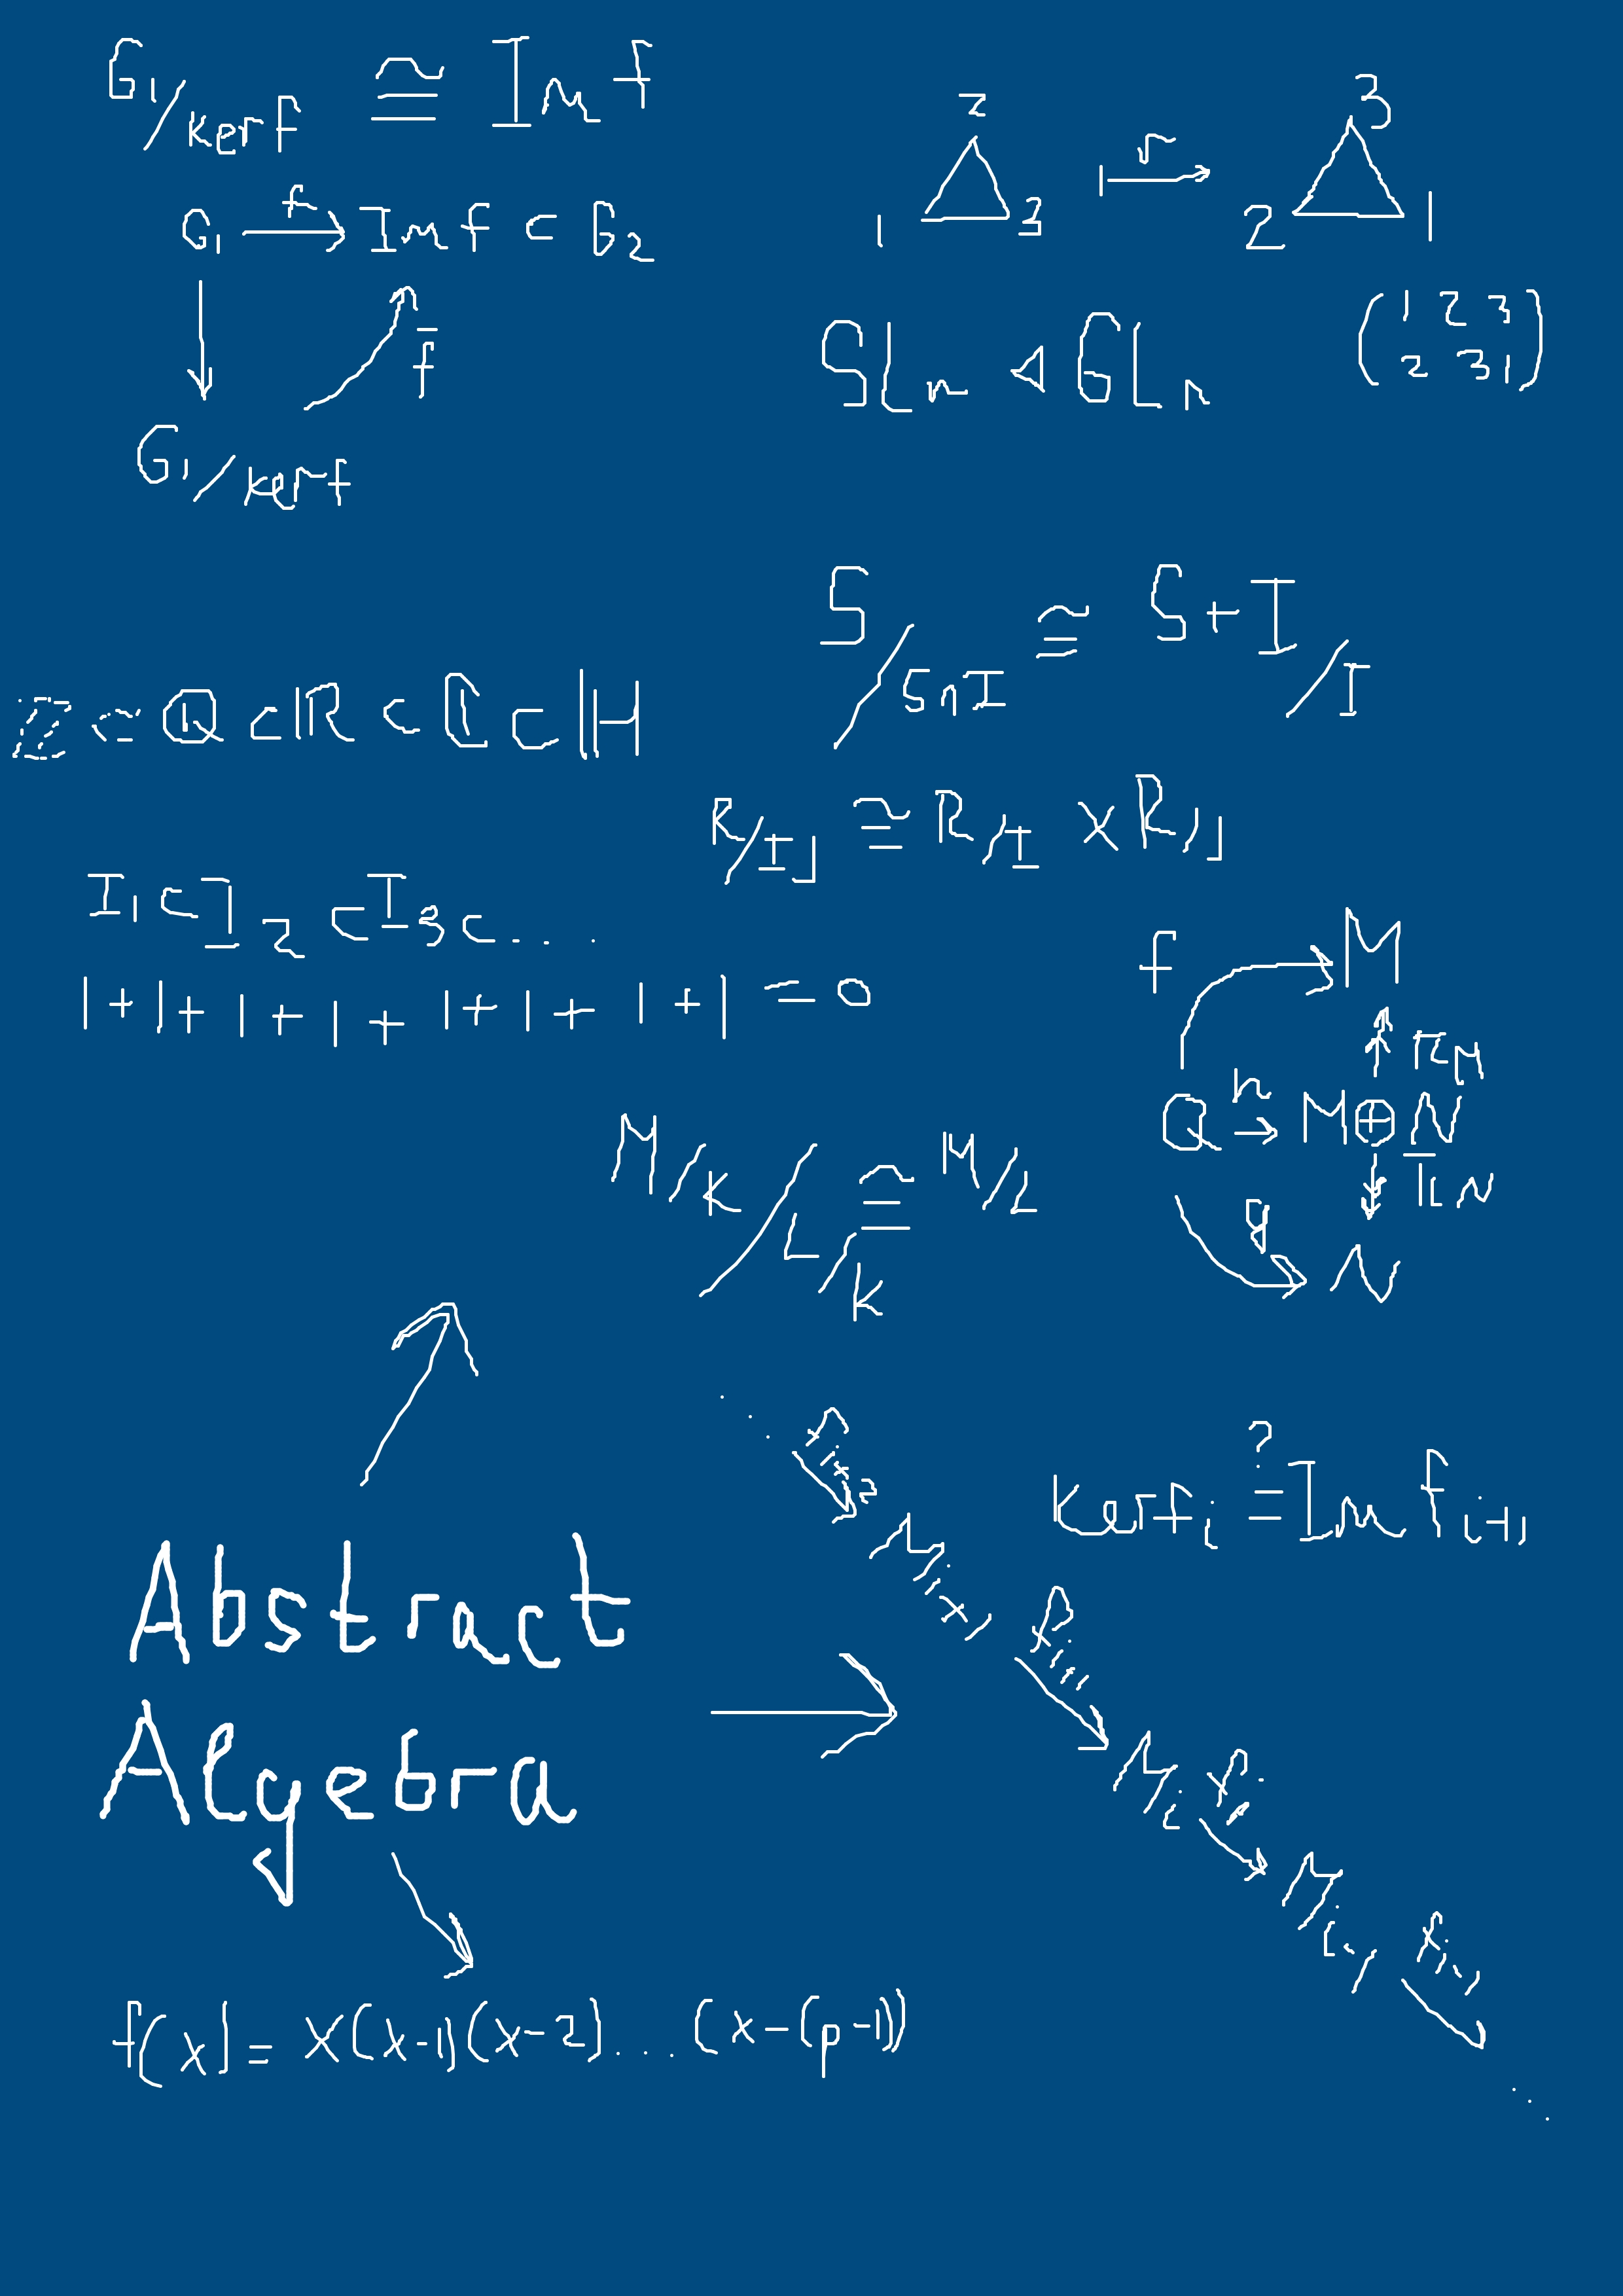
\includepdf[scale=1]{preview.jpg}

\tableofcontents
\newpage
\section*{Попередні знання, які необхідні}
Перед початком теорії груп наполегливо рекомендується згадати такі предмети:
\begin{itemize}[nosep,wide=0pt]
\item більшу частину теорії дискретної математики, як-от: теорія множин, відношень, трошки про відображення, трошки комбінаторики (останнє опціонально, але не завадить ніколи);
\item більшу частину теорії чисел, зокрема: вся теорія про подільність, теорія про конгруентні числа, базові відомості про функції Ойлера;
\item трошки теорії многочленів (залишив у PDF аналітичної геометрії);
\item частину лінійної алгебри, особливо матриці. Для нормального засвоєння розділу 5 дуже бажано мати відомості про векторні простори.
\end{itemize}
Третє не сильно принципово, оскільки ми покриємо ще раз теорію многочленів уже в загальному представленні. Але просто для простої орієнтації варто пройтися трошки.

\section*{Які розділи читати}
Нормальним людям потрібні лише розділи 1, 2, тому що вони зустрічаються в різних місцях (математикам я би ще рекомендував останній розділ для повної картини). Решта розділів --- це суто для тих, хто хоче детальніше знати, як облаштовані групи, або кому треба пройти теорію Галуа.
\newpage

% SECTION NAMES
%Теорія груп
%Теорія групової дії
%Просунуті матеріали з теорії груп
%Теорія кілець
%Зв'язок з теорією кілець та теорією чисел
%Многочлени
%Теорія модулів
%Модулі над областями цілісності
%Теорія полів
%Алгебра

% start Теорія груп
%\iffalse
\section{Теорія груп}
Я почну одразу з означення групи, хоча є деякі корисні терміни: алгебраїчна структура, оператив, моноїд тощо. Але основна мета цього розділу --- суто робота з групами, тому одразу даю більш розгорнуте означення.

\subsection{Означення груп}
\begin{definition}
Нехай $G$ --- деяка непорожня множина та $* \colon G \times G \to G$ --- деяка бінарна операція.\\
\textbf{Групою} назвемо пару $\left<G, *\right>$, для якої виконуються такі властивості:
\begin{enumerate}[nosep,label={\Roman*.}]
\item Замкненість відносно операції:
\begin{align*}
\forall a,b \in G: a*b \in G.
\end{align*}
\item Підпорядкована такими аксіомами:
\begin{align*}
\begin{tabular}{lll}
1) & $\forall a,b,c \in G: a*(b*c) = (a*b)*c;$ &  (асоціативність) \\
2) & $\exists e \in G: a*e = e*a = a;$ & (існування нейтрального елементу) \\
3) & $\forall a \in G: \exists a^{-1} \in G: a*a^{-1} = a^{-1}*a = e.$ & (існування оберненого елементу)
\end{tabular}
\end{align*}
\end{enumerate}
\end{definition}

Ніфіга неясно, що тут написано, тому радше наведу детальний приклад.

\begin{example}
Оберемо непорожню множину $G = \mathbb{R}$ (\textit{дійсні числа}) та візьмемо бінарну операцію $* \equiv + \colon \mathbb{R} \times \mathbb{R} \to \mathbb{R}$ (\textit{додавання цих чисел}). Структура $\left<\mathbb{R},+\right>$ задає групу.
\begin{enumerate}[wide=0pt,label={\Roman*)}]
\item Зі школи відомо, що якщо взяти будь-які числа $a,b \in \mathbb{R}$, то сума чисел буде теж числом, тобто $a+b \in \mathbb{R}$.

\item Далі відомо також зі школи, що:
\begin{enumerate}[nosep,label={\arabic*)}]
\item $a + (b + c) = (a + b) + c$ для будь-яких чисел $a,b,c \in \mathbb{R}$;
\item $a + 0 = a$ та $0 + a = a$, звідси число $e = 0 \in \mathbb{R}$ буде тим самим нейтральним елементом;
\item $a + (-a) = 0$ та $(-a) + a = 0$, звідси оберненим до $a \in \mathbb{R}$ відносно додавання (!) буде його протилежне число $-a \in \mathbb{R}$. 
\end{enumerate}
\end{enumerate}
(\textit{я знаю, що в школі казали, що $a^{-1} = \dfrac{1}{a}$, але це буде оберненим відносно множення}.)
\end{example}

\begin{example}
Можна ще деякі приклади розглянути:
\begin{itemize}
\item Якщо взяти ось цю структуру $\left< \mathbb{R} \setminus \{0\},\ \cdot \right>$, то це теж задає групу. Нейтральним елементом буде число $e = 1 \in \mathbb{R}$, а для кожного $a \in \mathbb{R} \setminus \{0\}$ оберненим відносно множення буде число $a^{-1} = \dfrac{1}{a}$ (\textit{як було в школі}).

\item Якщо взяти ось цю структуру $\left< \Mat_{n \times n}(\mathbb{R}),+\right>$, то це теж задає групу. Нейтральним елементом буде матриця $e = O$ (\textit{нульова матриця}), а для кожної $A \in \Mat_{n \times n}(\mathbb{R})$ оберненим відносно додавання буде матриця $A^{-1} = -A \in \Mat_{n \times n}(\mathbb{R})$ (\textit{протилежна матриця}).
\end{itemize}

(\textit{вправа: довести, що це дійсно групи})
\end{example}

\begin{example}
Ось така струткура $\left< \Mat_{n \times n}(\mathbb{R}),\ \cdot \right>$ уже не буде групою, оскільки порушується пункт ІІ 3): не для всіх матриць $A \in \Mat_{n \times n}(\mathbb{R})$ існує оберненої матриці $A^{-1}$ (\textit{при $\det A = 0$ нема оберненої}).
\end{example}

\textit{Позначення}: $\mathrm{GL}_n(\mathbb{R})$ --- множина матриць з $\Mat_{n \times n}(\mathbb{R})$ з ненульовими визначниками.\\
\textit{Позначення}: $\mathrm{SL}_n(\mathbb{R})$ --- множина матриць з $\mathrm{GL}_n$ з одиничними визначниками (\textit{пізніше знадобиться}).

\begin{example}
Структура $\left< \mathrm{GL}_n,\ \cdot \right>$ задає групу, яку ще називають \textbf{загальною лінійною групою}. Перевіримо це за означенням.

\begin{enumerate}[wide=0pt,label={\Roman*)}]
\item Нехай $A,B \in \mathrm{GL}_n$, тобто $\det A \neq 0,\ \det B \neq 0$. Із лінійної алгебри відома тотожність \[
\det (A \cdot B) = \det A \cdot \det B,
\] а тому звідси $\det (A \cdot B) \neq 0$ --- отримали $AB \in \mathrm{GL}_n$.

\item Перевіримо три аксіоми:
\begin{enumerate}[nosep,label={\arabic*)}]
\item Нехай $A,B,C \in \mathrm{GL}_n$, тоді звідси $A \cdot (B \cdot C) = (A \cdot B) \cdot C$ (\textit{асоціативність кожних трьох матриць виконується із лінійної алгебри}).
\item Існує матриця $I$ --- одинична матриця, причому $\det I = 1 \neq 0$, а тому $I \in \mathrm{GL}_n$ та $A \cdot I = I \cdot A = A$. Отже, $I$ буде нейтральним елементом.
\item Нехай $A \in \mathrm{GL}_n$, тобто $\det A \neq 0$. Значить, існує $A^{-1} = \frac{1}{\det A} \overline{A}$, де $\overline{A}$ --- приєднана матриця (\textit{див.~лінійну алгебру}), для якої $A \cdot A^{-1} = A^{-1} \cdot A = I$.
\end{enumerate}
\end{enumerate}
\end{example}

\begin{proposition}[Властивості єдиності]
Нехай $\left<G,* \right>$ --- група. Тоді:
\begin{enumerate}[nosep,wide=0pt, label={\arabic*)}]
\item існуючий нейтральний елемент $e \in G$ --- єдиний;
\item для кожного елемента $a \in G$ існуючий обернений елемент $a^{-1} \in G$ --- єдиний.
\end{enumerate}
\end{proposition}

\begin{proof}
\begin{enumerate}[topsep=0pt,wide=0pt,label={\arabic*)}]
\item Припустимо, що існують два нейтральні елементи: $e_1,e_2 \in G$. Отримуємо рівності: \[
e_1 = e_1*e_2, \qquad e_2 = e_1*e_2,
\] а тому звідси $e_1 = e_2$.

\item Припустимо, що для $a \in G$ існують два обернені $a_1^{-1},a_2^{-1} \in G$. Отримуємо ланцюг рівностей:
\[
a_1^{-1} = a_1^{-1} * e = a_1^{-1} * (a*a_2^{-1}) = (a_1^{-1}*a)*a_2^{-1} = e*a_2^{-1} = a_2^{-1}. \]
Одержали простенькі суперечності в двох випадках. \qedhere
\end{enumerate}
\end{proof}

\begin{proposition}[Додаткові властивості]
Нехай $\left<G,* \right>$ --- група. Тоді:
\begin{enumerate}[nosep,wide=0pt, label={\arabic*)}]
\item для кожного елемента $a \in G$ маємо $(a^{-1})^{-1} = a$;
\item для кожних $a,b \in G$ маємо $(a*b)^{-1} = b^{-1}*a^{-1}$;
\item рівняння $a*x = b$ має єдиний розв'язок $x=a^{-1}*b$;
\item $a*x = b*x \iff a = b$ (\textit{іншими словами, ми можемо скорочувати або домножувати обидві частини}).
\end{enumerate}
\textit{Вправа: довести всі властивості.}
\end{proposition}

\begin{definition}
Група $\left<G,* \right>$ називається \textbf{абелевою}, якщо
\begin{align*}
\forall a,b \in G: a*b = b*a. \qquad {\text{(комутативність)}}
\end{align*}
\end{definition}

\begin{example}
Зокрема групи $\left< \mathbb{R},+ \right>,\ \left< \mathbb{R} \setminus \{0\},\ \cdot \right>$ є абелевими.
\end{example}

\subsection{Степінь елемента}
\begin{definition}
Нехай $\left< G, * \right>$ --- група, $a \in G$ та $n \in \mathbb{N}$.\\
\textbf{Степенем елемента} $a$ назвемо наступне:
\begin{align*}
a^n = \underbrace{a*a*\dots*a}_{n \text{ разів}}; \\
a^{-n} = (a^{-1})^{n}; \\
a^0 = e.
\end{align*}
\end{definition}

\begin{remark}
На основі означення зробимо висновок, що оберненим до елемента $a^n$ буде елемент $a^{-n}$ при будь-якому $n \in \mathbb{Z}$, або, інакше кажучи,
\[
(a^n)^{-1} = a^{-n}.
\]
Дійсно, для цього доведемо, що $a^{-n}$ та $a^n$ при множенні дають нейтральний елемент.
\[
a^n * a^{-n} = a^n * (a^{-1})^n = \underbrace{a*a*\dots*a}_{n \text{ разів}} * \underbrace{a^{-1}*a^{-1}*\dots*a^{-1}}_{n \text{ разів}} = e.
\]
Згортати цей вираз треба починати з першого $a*a^{-1} = e$, далі так само повторюється до останнього.
\end{remark}

\begin{remark}
Крім того, рівність $a^{-n} = (a^{-1})^n$ виконується, насправді, для кожного $n \in \mathbb{Z}$ (\textit{не лише для натуральних чисел}).\\
Якщо $n = 0$, то цілком зрозуміло, що рівність виконується за означенням зведення в степінь нуль.\\
Якщо $n < 0$, то число $(-n)$ буде додатним, тоді маємо наступне:
\[
a^{-n} = ((a^{-1})^{-1})^{-n} = (a^{-1})^{-(-n)} = (a^{-1})^n.
\]
\end{remark}

\begin{proposition}[Властивості степеней]
Нехай $\left<G, *\right>$ --- група. Тоді для будь-яких $m,n \in \mathbb{Z}$ маємо:
\begin{enumerate}[nosep, wide=0pt, label={\arabic*)}]
\iffalse\textit{Аналогічно для $x*a=b$ та $x*a=x*b$ виконано}.\fi
\item $a^{m+n} = a^m*a^n$;
\item $(a^m)^n = a^{mn}$.
\end{enumerate}
\end{proposition}

\begin{proof}
Насправді, етапи доведення повторюються, як це було в шкільній алгебрі, якщо хтось цікавився доведеннями. Проте наведу повторно.
\begin{enumerate}[nosep, wide=0pt, label={\arabic*)}]
\item Для цього треба розглянути чимало випадків:
\begin{itemize}
\item \textit{Числа $m,n$ одночасно додатні}.\\
Тоді маємо таку рівність, користуючись асоціативністю:
\[
a^m * a^n = \underbrace{(a*a*\dots*a)}_{m \text{ разів}} * \underbrace{(a*a*\dots*a)}_{n \text{ разів}} = \underbrace{a*a*\dots*a}_{m+n \text{ разів}} = a^{m+n}.
\]
\item \textit{Числа $m,n$ одночасно від'ємні}.\\
Тоді $-m, -n$ одночасно додатні. Користуючись рівністю для попереднього випадку та означенням зведення в степінь, маємо уже таку рівність:
\[
a^m * a^n = (a^{-1})^{-m} * (a^{-1})^{-n} \overset{\text{попередній випадок}}{=} (a^{-1})^{-(m+n)} = a^{m+n}.
\]
\item \textit{Число $m$ додатне, а число $n$ від'ємне}.\\
Насправді, тут ще треба погратися з двома підвипадками:
\begin{itemize}[label={\#}]
\item $m+n > 0$.\\
Оскільки $m+n$ та $-n$ додатні, то користуємось формулою:
\[
a^{m} = a^{(m+n)-n} = a^{m+n} * a^{-n}.
\]
Далі обидві частини рівності помножимо на $a^n$ --- одержимо:
\[
a^m * a^n = a^{m+n}.
\]
\item $m+n < 0$.\\
Оскільки $m+n$ та $-m$ від'ємні, то користуємось формулою:
\[
a^{n} = a^{(m+n)-m} = a^{m+n} * a^{-m}.
\]
Далі обидві частини рівності помножимо на $a^m$ --- одержимо:
\[
a^m * a^n = a^{m+n}.
\]
\item $m+n = 0$.\\
Тоді $m = -n$, а тому рівність виконується автоматично.
\end{itemize}
\item \textit{Число $m$ від'ємне, а число $n$ додатне}.\\
Доведення тут аналогічне до попереднього пункту, тому пропускаю.
\item \textit{Число $m$ або число $n$ нульове, або одночасно двоє нульові}.\\
Тут, в цілому, нема що коментувати, все ясно.
\end{itemize}

\item Знову для цього будемо розбивати кілька випадків.
\begin{itemize}
\item \textit{Числа $m,n$ додатне}.\\
Тоді маємо таку рівність, користуючись уже відомою властивістю:
\[
(a^m)^n = \underbrace{a^m*a^m*\dots*a^m}_{n \text{ разів}} = a^{\scriptstyle\underbrace{\scriptstyle m+m+\dots+m}_{n \text{ разів}}} = a^{mn}.
\]
\item \textit{Числа $m,n$ одночасно від'ємні}.\\
Тоді $-m,-n$ стануть додатними, а далі весело:
\begin{align*}
(a^m)^{n} = ((a^{-1})^{-m})^{n} = (((a^{-1})^{-m})^{-1})^{-n} = ( (a^{-1})^{-(-m)} )^{-n} \\
= ((a^{-1})^m)^{-n} = (a^{-m})^{-n} = a^{(-m)(-n)} = a^{mn}.
\end{align*}
\item \textit{Число $m$ додатне, а число $n$ від'ємне}.\\
Маємо $-m$ уже від'ємне, а тоді буде наступне:
\[
(a^m)^{n} = ((a^{-1})^{-m})^n = (a^{-1})^{-mn} = a^{mn}.
\]
\item \textit{Число $n$ додатне, а число $m$ від'ємне}.\\
Співпадає з найпершим випадком.

\item \textit{Число $m$ або число $n$ нульове, або одночасно двоє нульові}.\\
Тут теж все цілком зрозуміло. \qedhere
\end{itemize}
\end{enumerate}
\end{proof}

\subsection{Деякі інші корисні групи}
\subsubsection{Групи лишків}
Розглянемо множину $\mathbb{Z}$ та будь-яке число $n \in \mathbb{N}$. Задамо відношення еківалентності:
\begin{align*}
x \sim y \iff x \equiv y \pmod n.
\end{align*}
Ми вже її якось встигли профакторизувати ось так (\textit{див.~дискретну математику}):
\begin{align*}
\mathbb{Z}/_{\!\!\pmod n} = \{[0],\ [1],\ \dots,\ [n-1] \},
\end{align*}
де елементами даної множини є класи еквівалентності:
\begin{align*}
[0] = \{\dots,-2n,-n,0,n,2n,\dots\}; \\
[1] = \{\dots, -2n+1,-n+1,1,n+1,2n+1,\dots\}; \\
\vdots \\
[n-1] = \{-n-1,-1,n-1,2n-1,3n-1),\dots\}.
\end{align*}
Зробимо перепозначення $[k] = \overline{k}$, а також $\mathbb{Z}/_{\!\!\pmod n} = \mathbb{Z}_n$.
\begin{definition}
Отримана фактормножина
\begin{align*}
\mathbb{Z}_n = \{\overline{0}, \overline{1}, \dots, \overline{n-1} \}, \\
\overline{k} = \{\dots,-2n+k,-n+k,k,n+k,2n+k,\dots\}
\end{align*}
називається \textbf{класом лишків за модулем $n$}.
\end{definition}

\begin{figure}[H]
\centering
\begin{tikzpicture}
\draw[dashed, black!30] (-1,-1.5) rectangle (7,1.5) node[scale=0.8, black] at (-0.8,1.3) {$\mathbb{Z}$};
\draw[dashed, black!30] (1.5,-1.5)--(1.5,1.5);
\draw[dashed, black!30] (4.5,-1.5)--(4.5,1.5);

\node[red] at (0,0) {$0$};
\node[red] at (0.5,0.5) {$-3$};
\node[red] at (0.7,-0.1) {$3$};
\node[red] at (0.1,-0.5) {$-6$};
\node[red] at (-0.5,-0.2) {$9$};
\node[red] at (-0.2,0.6) {$6$};
\node at (0,-1) {$\vdots$};
\node at (0,-2.2) {$\overline{0}$};
%0

\node[green] at (3,0) {$1$};
\node[green] at (3.5,0.5) {$-2$};
\node[green] at (3.7,-0.1) {$4$};
\node[green] at (3.1,-0.5) {$-5$};
\node[green] at (2.5,-0.2) {$10$};
\node[green] at (2.8,0.6) {$7$};
\node at (3,-1) {$\vdots$};
\node at (3,-2.2) {$\overline{1}$};
%1

\node[blue] at (6,0) {$2$};
\node[blue] at (6.5,0.5) {$-1$};
\node[blue] at (6.7,-0.1) {$5$};
\node[blue] at (6.1,-0.5) {$-4$};
\node[blue] at (5.5,-0.2) {$11$};
\node[blue] at (5.8,0.6) {$8$};
\node at (6,-1) {$\vdots$};
\node at (6,-2.2) {$\overline{2}$};
%2
\end{tikzpicture}
\caption*{На прикладі проілюстрував множину $\mathbb{Z}_3 = \{ \overline{0}, \overline{1}, \overline{2} \}$.}
\end{figure}

\begin{theorem}
$\left<\mathbb{Z}_n, + \right>$ задає абелеву групу\footnote{Забігаючи наперед, ми щойно побудували так звану факторгрупу. Я міг би цей приклад групи засунути аж в майже самий кінець цього розділу, проте не можу, тому що така група генерує чимало важливих прикладів.}, де операція визначається таким чином: \[
\overline{a}+\overline{b} \eqbydef \overline{a+b}.
\]
\end{theorem}

\begin{proof}
\begin{enumerate}[topsep=0pt,wide=0pt,label={\Roman*.}]
\item \textit{Коректність визначеної операції}.\\
Нехай $\overline{a} = \overline{c}$ та $\overline{b} = \overline{d}$. Хочемо довести, що $\overline{a+b} = \overline{c+d}$.\\
%Паралель: 1/2 = 2/4 та 1/3 = 3/6, тоді треба пересвідчитись, що 1/2+1/3 = 5/6 - це той самий елемент, що й 2/4 + 3/6 = 10/12
Маємо $a \equiv c \pmod n$ та $b \equiv d \pmod n$. А тому за властивостями конгруенції (\textit{див.~ теорію чисел}), $a+b \equiv c+d \pmod n$. Тобто $\overline{a+b} = \overline{c+d}$.

\item \textit{Доведення факту, що це --- абелева група}.
\begin{enumerate}[nosep,wide=0pt,label={\roman*.}]
\item Для кожного $\overline{a},\ \overline{b} \in \mathbb{Z}_n$ ми вже маємо $\overline{a}+\overline{b} = \overline{a+b} \in \mathbb{Z}_n$ --- тобто замкненість є, бо отримали, по суті, клас еквівалентності.
\item Перевіримо аксіоми груп:
\begin{enumerate}[nosep,label={\arabic*)}]
\item нехай $\overline{a},\ \overline{b},\ \overline{c} \in \mathbb{Z}_n$. Тоді маємо: \[
\overline{a}+(\overline{b}+\overline{c}) = \overline{a}+\overline{b+c} = \overline{a+(b+c)} = \overline{(a+b)+c} = \overline{a+b} + \overline{c} = (\overline{a}+\overline{b})+\overline{c},\]
тобто асоціативність є;
\item нейтральним елементом стане $\overline{0} \in \mathbb{Z}_p$, тому що 
\[
\overline{a} + \overline{0} = \overline{a+0} = \overline{a};
\]
\item для $\overline{a} \in \mathbb{Z}_n$ оберненим елементом стане $\overline{a}^{-1} = \overline{p-a}$, бо 
\[
\overline{a} + \overline{a}^{-1} = \overline{a} + \overline{p-a} = \overline{a+p-a} = \overline{p} = \overline{0}.
\]
\end{enumerate}
\item Комутативність даної групи виконується, оскільки для кожного $\overline{a},\overline{b} \in \mathbb{Z}_n$ маємо 
\[
 \overline{a} + \overline{b} = \overline{a+b} = \overline{b+a} = \overline{b} + \overline{a}. \qedhere 
 \]
\end{enumerate}
\end{enumerate}
\end{proof}

\begin{example}
Існує так звана \textbf{таблиця Келі}, покажу на прикладі $\left<\mathbb{Z}_3,+ \right>$.
\begin{figure}[H]
\centering
\begin{tabular}{c|ccc}
$+$ & $\overline{0}$ & $\overline{1}$ & $\overline{2}$ \\ 
\hline \\ [-9pt]
$\overline{0}$ & $\overline{0}$ & $\overline{1}$ & $\overline{2}$ \\ 
$\overline{1}$ & $\overline{1}$ & $\overline{2}$ & $\overline{0}$ \\
$\overline{2}$ & $\overline{2}$ & $\overline{0}$ & $\overline{1}$ \\
\end{tabular}
\end{figure}
Фактично кажучи, таблиця Келі описує всі можливі (\textit{у цьому випадку}) додавання між двома об'єктами та їхні результати.
\end{example}

\begin{theorem}
\label{multiplicative_class_of_residues_mod_n_is_a_group}
$\left< \mathbb{Z}_p \setminus \{\overline{0}\},\ \cdot \right>$, де $p$ --- просте число, задає абелеву група, де операція визначається таким чином: \[
\overline{a} \cdot \overline{b} \overset{\text{def.}}{=} \overline{a \cdot b}. \]
\end{theorem}

Перед доведенням теореми прокоментую кілька обмежень.
\begin{enumerate}[wide=0pt,label={\Roman*.}]
\item \textit{Чому вилучили елемент $\overline{0}$}?\\
Розглянемо структуру $\left< \mathbb{Z}_p, \cdot \right>$. Вона задовольняє умови 1) та 2) (\textit{нейтральним елементом буде $\overline{e} = \overline{1}$}). Але умова 3) не виконується, тому що елемент $\overline{0} \in \mathbb{Z}_p$ не має оберненого. Адже якби $\overline{0} \in \mathbb{Z}_p$ містив обернений $\overline{a} \in \mathbb{Z}_p$, то ми би одержали $\overline{0} \cdot \overline{a} = \overline{1}$ з одного боку та $\overline{0} \cdot \overline{a} = \overline{0}$ з іншого боку, тобто $\overline{0} = \overline{1}$ --- неможливо.

\item \textit{Чому $p$ має бути простим числом}?\\
Розглянемо структуру $\left<\mathbb{Z}_p \setminus \{\overline{0}\}, \cdot \right>$, де $p$ --- складене. Цього разу оскільки $p$ --- складене, то існує якийсь інший дільник $1 < n < p$. Тому звідси $p = nm$, внаслідок чого $\overline{p} = \overline{n} \cdot \overline{m}$. Проте $\overline{p} = \overline{0}$, а тому $\overline{n}\cdot \overline{m} = \overline{0}$. Це означає, що хоча $\overline{m}, \overline{n} \in \mathbb{Z}_p$, але $\overline{mn} = \overline{0} \not\in \mathbb{Z}_p$. Замкненості нема.
\end{enumerate}

Тепер повернімося до теореми та доведемо її.
\begin{proof}
\begin{enumerate}[topsep=0pt,wide=0pt,label={\Roman*.}]
\item \textit{Коректність визначеної операції}.\\
Нехай $\overline{a} = \overline{c}$ та $\overline{b} = \overline{d}$. Хочемо довести, що $\overline{ab} = \overline{cd}$.\\
Маємо $a \equiv c \pmod p$ та $b \equiv d \pmod p$. А тому за властивостями конгруенції (\textit{див.~теорію чисел}), $ab \equiv cd \pmod p$. Тобто $\overline{ab} = \overline{cd}$.

\item \textit{Доведення факту, що це --- абелева група}.
\begin{enumerate}[nosep,wide=0pt,label={\roman*.}]
\item Доведемо, що $\overline{a} \cdot \overline{b} \in \mathbb{Z}_p \setminus \{ \overline{0}\}$ для всіх $\overline{a},\ \overline{b} \in \mathbb{Z}_p \setminus \{ \overline{0}\}$.\\
!Припустимо $\overline{a} \cdot \overline{b} \not\in \mathbb{Z}_p \setminus \{ \overline{0}\}$, тоді єдиний варіант --- це $\overline{a} \overline{b} = \overline{ab} = \overline{0}$, тобто $p \mid ab$. А оскільки $p$ --- просте, то звідси або $p \mid a$, або $p \mid b$. У двох випадках отримаємо суперечність!\\
Отже, замкненість успішно виконується.

\item Тепер доведемо виконання аксіом груп.
\begin{enumerate}[nosep,label={\arabic*)}]
\item нехай $\overline{a},\ \overline{b},\ \overline{c} \in \mathbb{Z}_n$. Тоді маємо: 
\[
\overline{a}(\overline{b}\overline{c}) = \overline{a}\overline{bc} = \overline{a(bc)} = \overline{(ab)c} = \overline{ab} \overline{c} = (\overline{a}\overline{b})\overline{c},
\]
тобто асоціативність є.
\item нейтральним елементом стане $\overline{1} \in \mathbb{Z}_p \setminus \{ \overline{0}\}$, тому що
\[ 
\overline{a} \cdot \overline{1} = \overline{a \cdot 1} = \overline{a}.
\]
\item а ось з оберненим елементом ситуація складніша. Маємо $\overline{a} \in \mathbb{Z}_p \setminus \{ \overline{0}\}$, розглянемо ось таку множину: 
\[ 
\{\overline{a},\ \overline{2a},\ \dots,\ \overline{(p-1)a} \}. 
\]
Спочатку покажемо, що тут всі елементи абсолютно різні. \\
!Припускаючи, що $\overline{k_1 a} = \overline{k_2 a}$ для $k_1 \neq k_2$, ми отримаємо 
\[ 
k_1 a \equiv k_2 a \pmod p \implies (k_1-k_2)a \equiv 0 \pmod p.
\] 
У силу того, що $p$ --- просте, то або $p \mid a$, що точно неправда, або $p \mid k_1-k_2$. Але це має місце лише тоді, коли $k_1 = k_2$, оскільки $k_1,k_2 = \overline{1,p-1}$. Суперечність!\\
Отже, множина $\{\overline{a},\ \overline{2a},\ \dots,\ \overline{(p-1)a} \}$ містить різні елементи. Так само різні елементи містить $\mathbb{Z}_p \setminus \{ \overline{0}\}$, тобто фактично ми отримали, що 
\[
\{\overline{a},\ \overline{2a},\ \dots,\ \overline{(p-1)a} \} = \{ \overline{1}, \overline{2}, \dots, \overline{p-1} \} = \mathbb{Z}_p \setminus \{ \overline{0}\}.
\]
Таким чином, елемент серед елементів $\overline{ka}$, де $k = 1,2,\dots,p-1$, має бути елемент $\overline{1}$. Тоді для $\overline{a} \in \mathbb{Z}_p \setminus \{ \overline{0}\}$ знайдеться деякий $\overline{ka}$, для якого $\overline{ka} = \overline{k} \overline{a} = \overline{1}$, і от $\overline{k}$ буде деяким оберненим елементом.
\end{enumerate}

\item Комутатинвість даної групи виконується, оскільки для кожних $\mathbb{Z}_p \setminus \{ \overline{0}\}$ маємо
\[
\overline{a} \overline{b} = \overline{ab} = \overline{ba} = \overline{b} \overline{a}. \qedhere
\]
\end{enumerate}
\end{enumerate}
\end{proof}

\begin{example}
Тут теж будується \textbf{таблиця Келі}, покажу на $\left<\mathbb{Z}_5 \setminus \{\overline{0}\},\ \cdot \right>$.
\begin{figure}[H]
\centering
\begin{tabular}{c|cccc}
$\cdot$ & $\overline{1}$ & $\overline{2}$ & $\overline{3}$ & $\overline{4}$ \\
\hline \\ [-9pt]
$\overline{1}$ & $\overline{1}$ & $\overline{2}$ & $\overline{3}$ & $\overline{4}$ \\
$\overline{2}$ & $\overline{2}$ & $\overline{4}$ & $\overline{1}$ & $\overline{3}$ \\
$\overline{3}$ & $\overline{3}$ & $\overline{2}$ & $\overline{4}$ & $\overline{2}$ \\
$\overline{4}$ & $\overline{4}$ & $\overline{3}$ & $\overline{2}$ & $\overline{1}$ \\
\end{tabular}
\end{figure}
Аналогічно таблиця Келі описує всі можливі множення між двома об'єктами та їхні результати. І ось тут таблиця Келі має сенс, тому що під час доведення ми не знайшли явної формули знаходження оберненого елементу, тому варто будувати табличку.
\end{example}

Повернімось назад до структури $\left< \mathbb{Z}_n \setminus \{\overline{0}\},\ \cdot \right>$, де $n \in \mathbb{N}$, що вже має нейтральний елемент $\overline{e} = \overline{1}$.

\begin{lemma}
\label{when_residue_class_is_invertible_in_mulitplicative_class}
$\overline{m} \in \mathbb{Z}_n \setminus \{ \overline{0} \}$ має обернений елемент $\iff \gcd(m,n) = 1$.
\end{lemma}

\begin{proof}
\rightproof Дано: $\overline{m} \in \mathbb{Z}_n \{\overline{0}\}$ має обернений, тобто існує $\overline{x} \in \mathbb{Z}_n \setminus \{\overline{0}\}$, для якого $\overline{m} \cdot \overline{x} = \overline{1}$. Тобто $mx \equiv 1 \pmod n$ для деякого $x$. Із курсу теорії чисел, можемо сказати, що $\gcd(m,n) \mid 1 \implies \gcd(m,n) = 1$.
\bigskip \\
\leftproof Дано: $\gcd(m,n) = 1$, тоді рівняння $mx \equiv 1 \pmod n$ матиме єдиний розв'язок $x$, із курсу теорії чисел. Мовою класів лишків, маємо $\overline{mx} = \overline{m} \cdot \overline{x} = \overline{1}$. Таким чином, $\overline{m} \in \mathbb{Z}_n$ має обернений.
\end{proof}

Познайомимось з ось такою множиною: 
\[ 
U_n = \{ \overline{m} \in \mathbb{Z}_n \mid \gcd(m,n) = 1 \}.
\]

\begin{example}
$U_9 = \{\overline{1},\overline{2},\overline{4},\overline{5},\overline{7},\overline{8} \}$.
\end{example}

\begin{theorem}
$\left<U_n,\ \cdot \right>$ задає абелеву група з операцією $\cdot$ як було в $\mathbb{Z}_n \setminus \{ \overline{0} \}$.
\end{theorem}

\begin{proof}
\begin{enumerate}[nosep,wide=0pt,label={\roman*.}]
\item Із теорії чисел, відомо, що коли $\gcd(a,n) = 1,\ \gcd(b,n) = 1$, то звідси $\gcd(ab,n) = 1$. Тому одержимо, що $\overline{ab} \in U_n$ для будь-яких $\overline{a},\ \overline{b} \in U_n$.

\item Комутативність, асоціативність аналогічно доводиться, як і в \thref{multiplicative_class_of_residues_mod_n_is_a_group}. Нейтральний елемент досі $\overline{e} = \overline{1}$. Кожний елемент має обернений, бо $\overline{m} \in U_n \implies \gcd(m,n) = 1$. Тут спрацьовує \lmref{when_residue_class_is_invertible_in_mulitplicative_class}. \qedhere
\end{enumerate}
\end{proof}

\subsubsection{Групи кватерніонів}
Розглядається ось така множина:
\begin{align*}
Q_8 = \{1,-1,i,-i,j,-j,k,-k\}
\end{align*}
з операцією $\cdot$, яка працює ось таким чином:
\begin{align*}
i^2 = j^2 = k^2 = -1, \\
ijk = -1.
\end{align*}
(\textit{тут числа $1,-1$ --- дійсні числа, тобто множимо їх так, як звикли}).

\begin{theorem}
$\left<Q_8,\ \cdot \right>$ задає групу.\\
\textit{Вправа: довести}.
\end{theorem}

\iffalse
\begin{proof}
На основі заданих правил, можна отримати ще такі співвідношення:
\begin{align*}
ij = k, \qquad ji = -k, \\
jk = i, \qquad kj = -i, \\
ki = j, \qquad ik = -j.
\end{align*}
Дійсно,
\begin{align*}
ij = (-ij) (-1) = (-ij) k^2 = -(ijk)k = -(-1)k = k, \\
ji = ji (1) = ji (-ijk) = -(ji ijk) = -k.
\end{align*}
На прикладі першого було пояснення.
\begin{figure}[H]
\centering
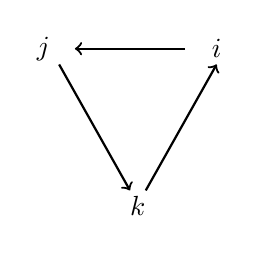
\begin{tikzpicture}
\draw[->, thick] (1.1,0.2)--(2,1.8) node at (2,2) {$i$};
\draw[->, thick] (1.6,2)--(0.2,2) node at (-0.2,2) {$j$};
\draw[->, thick] (0,1.8)--(0.9,0.2) node at (1,0) {$k$};
\end{tikzpicture}
\end{figure}
Із цього випливає замкненість операції множення.\\
Покажемо асоціативність, тобто $x(yz) = (xy)z$.\\
Не втрачаючи загальності, припустимо $x = i$. Ми будемо розглядати випадки $y,z \in \{i,j,k\}$ --- загалом $9$ варіантів. Із одиницею всередині все зрозуміло, а мінусові не беремо, бо все те саме з точністю до знака. Якщо всі варіанти розписати, то можна переконатись в рівностях.\\
Нейтральним елеемнтом буде $1$.\\
Залишились обернені елементи:
\begin{figure}[H]
\centering
\begin{tabular}{c|c}
$a$ & $a^{-1}$ \\
\hline
$\pm 1$ & $\pm 1$ \\
$i$ & $-i$ \\
$j$ & $-j$ \\
$k$ & $-k$
\end{tabular}
\end{figure}
Не повністю розписано, але тим не менш доведено.
\end{proof}
\fi

\subsubsection{Симетричні групи}
\begin{definition}
\textbf{Перестановкою} елементів множини $X \neq \emptyset$ називають бієкцію 
\begin{align*}
\sigma \colon X \to X.
\end{align*}
\textit{Позначення}: $S_X$ --- множина всіх перестановок на множині $X$.
\end{definition}

\begin{theorem}
$\left< S_X, \circ \right>$ задає групу при $X \neq \emptyset$.
\end{theorem}

Спершу зазначимо, що композиція будь-яких відображень --- асоціативна, а нейтральним елементом буде відображення $\id \colon X \to X$, що задається як $\id(x) = x$ для всіх $x \in X$, яке є бієкцією (\textit{тобто $\id \in S_X$}). Залишилось довести замкненість операції та існування оберненого. Для цього наведу леми.

\begin{lemma}[Про замкненість]
Нехай $\sigma, \mu \colon X \to X$ --- бієкції. Тоді $\sigma \circ \mu$ --- бієкція \\
(\textit{іншими словами, якщо $\sigma, \mu \in S_X$, то звідси $\sigma \circ \mu \in S_X$}).
\end{lemma}

\begin{proof}
\begin{enumerate}[topsep=0pt,label={\Roman*.},wide=0pt]
\item \textit{$\sigma \circ \mu$ --- ін'єктивне}.\\
Припустимо маємо $a \neq b$, але $\sigma \circ \mu (a) = \sigma \circ \mu (b)$. Тобто звідси \[
\sigma (\mu(a)) = \sigma (\mu(b)) \implies \mu(a) = \mu(b) \implies a = b.
\]
Отримали суперечність від припущення, що $\sigma \circ \mu$ --- неін'єктивне. Отже, $\sigma \circ \mu$ все ж таки ін'єктивне.

\item \textit{$\sigma \circ \mu$ --- сюр'єктивне}.\\
Маємо $u \in X$, тоді існує $a \in X$, для якого $\sigma(a) = u$. Водночас для $a \in X$ існує $k \in X$, для якого $\mu(k) = a$. Отже, $\sigma \circ \mu (k) = \sigma(\mu(k)) = \sigma(a) = u$. \qedhere
\end{enumerate}
\end{proof}

\begin{lemma}[Про існування оберненого елементу]
Нехай $\sigma \colon X \to X$ --- бієкція. Тоді існує бієкція $\mu \colon X \to X$, для якого 
\[
\sigma(a) = b \iff \mu(b) = a
\]
(\textit{іншими словами, якщо $\sigma \in S_X$, то існує $\mu \in S_X$, для якого $\sigma \circ \mu(b) = b$ та $\mu \circ \sigma(a) = a$ для всіх $a,b \in X$, або що теж саме, що $\sigma \circ \mu = \id$ та $\mu \circ \sigma = \id$}).
\end{lemma}

\begin{proof}
\begin{enumerate}[topsep=0pt,label={\Roman*.},wide=0pt]
\item \textit{$\mu$ --- коректно визначено}.\\
Дійсно, якщо $\mu(b) = a_1$ та $\mu(b) = a_2$, то отримаємо звідси \[
\sigma(a_1) = b, \sigma(a_2) = b \implies a_1 = a_2.
\]

\item \textit{$\mu$ --- ін'єктивне}.\\
!Припустимо $b_1 \neq b_2$, але $\mu(b_1) = \mu(b_2)$. Позначимо $a_1 = \mu(b_1)$ та $a_2 = \mu(b_2)$. Тоді $b_1 = \sigma(a_1)$ та $b_2 = \sigma(a_2)$, а тому $b_1 = \sigma(a_1) = \sigma(a_2) = b_2$. Суперечність!

\item \textit{$\mu$ --- сюр'єктивне}.\\
Для кожного $a \in X$ існує елемент $b = \sigma(a)$, для якого $\mu(\sigma(a)) = a$. \qedhere
\end{enumerate}
\end{proof}

\subsubsection{Дієдричні групи}
\begin{definition}
\textbf{Дієдричною групою} називають групу $\left< S_{F}, \circ \right>$, де $F$ --- правильний многокутник. Тобто маємо набір рухів над правильним многокутником, причому його образом буде та сама фігура.\\
\textit{Позначення}: $D_n$, якщо маємо правильний $n$-кутник\footnote{Часто ще кажуть група дієдра. Крім того, замість $D_n$ можна часто бачити позначення $D_{2n}$. Перше позначення, як на мене, зручніше, оскільки пояснює, над яким $n$-кутником проводимо симетрії.}.
\end{definition}

Розглянемо правильний $n$-кутник.
\begin{figure}[H]
\centering
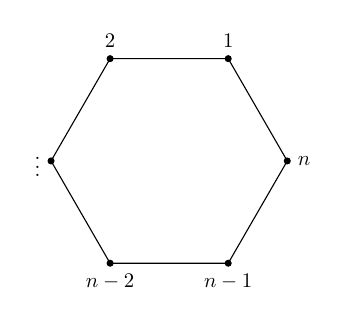
\begin{tikzpicture}[scale=0.75, transform shape]
   \newdimen\R
   \R=2cm
   \draw (0:\R) \foreach \x in {60,120,...,360} {  -- (\x:\R) };
   \foreach \x/\l/\p in
     { 60/{1}/above,
      120/{2}/above,
      180/{$\vdots$}/left,
      240/{$n-2$}/below,
      300/{$n-1$}/below,
      360/{$n$}/right
     }
     \node[inner sep=1pt,circle,draw,fill,label={\p:\l}] at (\x:\R) {};
\end{tikzpicture}
\end{figure}
\textit{Позначення}: $e$ --- тотожне перетворення правильного $n$-кутника.
Цілком зрозуміло, що таке перетворення $e \in D_n$.
\bigskip \\
\textit{Позначення}: $r$ --- поворот правильного $n$-кутника відносно його центра проти годинникової стрілки. Власне кажучи, $r$ описує поворот на $\dfrac{360^\circ}{n}$.\\
Зауважимо, що в цьому випадку $r \in D_n$. Крім того, можна зробити даний поворот двічі, тобто $r^2 \in D_n$, або тричі, тобто $r^3 \in D_n$. Але таких поворотів всього $(n-1)$ штука. Якщо провести $n$ таких поворотів, то многокутник повернеться в початкове положення. Якщо повернути один многокутник за годинниковою стрілкою на $\dfrac{360^\circ}{n}$, то це теж саме, що провести $(n-1)$ разів поворот на $\dfrac{360^\circ}{n}$ проти годинникової стрілки.
\bigskip \\
\textit{Позначення}: $s$ --- відбиття відносно деякої осі, що проходить через центр правильного $n$-кутника.
\begin{itemize}[nosep,wide=0pt]
\item якщо $n$-кутник має непарну кількість вершин, то в нас існують $n$ штук відбиття $s_1,s_2,\dots,s_n$, де $s_1$ --- відбиття відносно осі, яка проходить через центр та з'єднує першу вершину $n$-кутника;
\item якщо $n$-кутника має парну кількість вершин, то в нас $\dfrac{n}{2}$ штук відбиття $s_1,s_2,\dots,s_{\frac{n}{2}}$, де $s_1$ --- відбиття відносно осі, яка проходить через центр та з'єднує протилежні вершини $n$-кутника; але також в нас $\dfrac{n}{2}$ штук відбиття $s_{\frac{n}{2}+1},\dots,s_{n}$, де $s_{\frac{n}{2}+1}$ --- відбиття відносно осі, яка проходить через центр та з'єднує середини протилежних сторін $n$-кутника.3
\end{itemize}

Над цією фігурою можна зробити ось такі рухи:
\begin{enumerate}[nosep,wide=0pt,label={\arabic*)}]
\item обертання відносно центра фігури проти годинникової стрілки;
\item відбиття відносно осі, що проходить через центр фігури.
\end{enumerate}


\begin{theorem}
Зробимо деякі позначення:\\
$r$ --- поворот $n$-кутника на кут $\dfrac{360^\circ}{n}$ проти годинникової стрілки; \\
$s$ --- відбиття відносно деякої вісі симетрії;\\
$e$ --- тотожна дія (\textit{коротше, нічого не робимо з цією фігурою}).\\
(\textit{$r$ чи $s$ в деякому степені означає дану кількість разів застосувати відповідне перетворення}).\\
Тоді дієдрична група матиме такий вигляд:
\begin{align*}
D_n = \{ \underbrace{e,\ r,\ r^2,\ \dots,\ r^{n-1}}_{\text{обертання}},\ \underbrace{s,\ rs,\ r^2s,\ \dots,\ r^{n-1}s}_{\text{відбиття}} \},
\end{align*}
причому $\card D_{n} = 2n$, а також справедливі такі рівності:
\begin{align*}
r^n = e, \qquad s^2 = e, \qquad rs = sr^{n-1}.
\end{align*}

\end{theorem}

\begin{figure}[H]
\centering
\begin{tikzpicture}[scale=0.75, transform shape]
   \newdimen\R
   \R=2cm
   \draw (0:\R) \foreach \x in {60,120,...,360} {  -- (\x:\R) };
   \foreach \x/\l/\p in
     { 60/{1}/above,
      120/{2}/above,
      180/{$\vdots$}/left,
      240/{$n-2$}/below,
      300/{$n-1$}/below,
      360/{$n$}/right
     }
     \node[inner sep=1pt,circle,draw,fill,label={\p:\l}] at (\x:\R) {};
     
     \draw[->] (4,0)--(5,0) node[anchor = south east] {$r$};
     \node[white] at (0,-2.8) {$.$};
\end{tikzpicture}
\qquad
\begin{tikzpicture}[scale=0.75, transform shape]
   \newdimen\R
   \R=2cm
   \draw (0:\R) \foreach \x in {60,120,...,360} {  -- (\x:\R) };
   \foreach \x/\l/\p in
     { 60/{$n$}/above,
      120/{1}/above,
      180/{2}/left,
      240/{$\ddots$}/below,
      300/{$n-2$}/below,
      360/{$n-1$}/right
     }
     \node[inner sep=1pt,circle,draw,fill,label={\p:\l}] at (\x:\R) {};
     \node[white] at (0,-2.8) {$.$};
\end{tikzpicture}
\end{figure}

\begin{figure}[H]
\centering
\begin{tikzpicture}[scale=0.75, transform shape]
   \newdimen\R
   \R=2cm
   \draw (0:\R) \foreach \x in {60,120,...,360} {  -- (\x:\R) };
   \foreach \x/\l/\p in
     { 60/{1}/above,
      120/{2}/above,
      180/{$\vdots$}/left,
      240/{$n-2$}/below,
      300/{$n-1$}/below,
      360/{$n$}/right
     }
     \node[inner sep=1pt,circle,draw,fill,label={\p:\l}] at (\x:\R) {};
     \draw[red,dashed] (0,-2.2)--(0,2.2);
     
     \draw[->] (4,0)--(5,0) node[anchor = south east] {$s$};
\end{tikzpicture}
\qquad
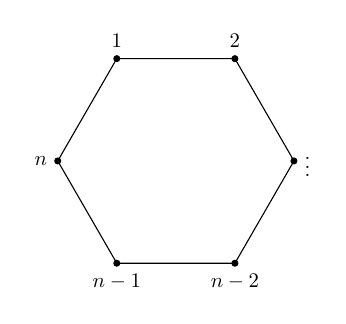
\begin{tikzpicture}[scale=0.75, transform shape]
   \newdimen\R
   \R=2cm
   \draw (0:\R) \foreach \x in {60,120,...,360} {  -- (\x:\R) };
   \foreach \x/\l/\p in
     { 60/{2}/above,
      120/{1}/above,
      180/{$n$}/left,
      240/{$n-1$}/below,
      300/{$n-2$}/below,
      360/{$\vdots$}/right
     }
     \node[inner sep=1pt,circle,draw,fill,label={\p:\l}] at (\x:\R) {};
\end{tikzpicture}
\end{figure}


\begin{proof}
Ясно, що $r^n = e$, оскільки ми повернемось до початкового положення, повертаючи на $360^\circ$.
\bigskip \\
\textit{Чому для правильних $n$-кутників всього рівно $n$ вісів симетрій?}\\
Візьмемо якусь одну вісь та зробимо відбиття. Ясно, що $s^2 = e$, тобто ми повернемось до початкового положення. Інші $(n-1)$ відбиття, які є в $n$-кутнику, виражаються через обраний вісь відбиття $s$ та певну кількість обертань $r$, тобто маємо:
\[
s,\ rs,\ r^2s,\ \dots,\ r^{n-1}s.
\]
\textit{Кожний елемент тут не є поворотом}.\\
Якби $r^l = r^ks$, то було б $s = r^{l-k}$, що неможливо: симетрія змінює орієнтацію, а обертання --- ні.
\bigskip \\
\textit{Всі ці відбиття різні}.\\
Якби $r^k s = r^l s$, то було б обов'язоко $r^k = r^l$, що неможливо при $k \neq l$.
\bigskip \\
Із цих міркувань ми робимо висновок, що нам неважливо, який вісь відбиття треба брати.
\bigskip \\
Зауважимо, що $(rs)^2 = e$, тобто $rs \cdot rs = e$, але тоді $r^{n-1} (rs \cdot rs) = r^{n-1}$, ми би одержали $s \cdot rs = r^{n-1}$. Нарешті, зробимо $s \cdot (srs) = sr^{n-1}$, тобто одержимо $rs = sr^{n-1}$.
\end{proof}

% TODO перенести
\iffalse
Можна ще переписати це як $D_n = [s,r]$.
\fi

\begin{theorem}
$\left< D_n,\ \circ \right>$ справді задає групу. (\textit{тут операцією $\circ$ є композиція дій на $n$-кутник, яку я хотів би далі явно не писати}).
\end{theorem}

\iffalse
\begin{proof}
Замкненість випливає з виразів $r^n = e, s^2 = e, r^ms = sr^{n-m}$. В останньому виразі ми користуватись властивістю асоціативності. І маємо на це права, бо композиція відображень завжди асоціативна.\\
Нейтральний елемент тут $e$ - нічого не робить з $n$-кутником.\\
Оборотні елементи для $r^k$ маємо $(r^{k})^{-1} = r^{n-k}$; для $r^k s$ маємо $(r^k s)^{-1} = s r^{-k} = s(r^k)^{-1}$.
\end{proof}
\fi

\begin{remark}
$\left< D_n, \circ \right>$ --- не абелева група в загальному випадку, принаймні тому що $sr \neq rs$.
\end{remark}

\subsubsection{Групи перестановок}
Один з найпоширеніших симетричних груп --- це група $\left<S_{\{1,2,\dots,n\}}, \circ \right>$, це ще пишуть як $\left<S_n, \circ \right>$.\\
Перестановки $\sigma \colon \{1,2,\dots,n\} \to \{1,2,\dots,n\}$ мають ще таке позначення:
\[
 \sigma = \begin{pmatrix}
1 & 2 & \dots & n \\
i_1 & i_2 & \dots & i_n
\end{pmatrix},
\]
де $\{i_1,i_2,\dots,i_n\}$ --- переставлені числа $\{1,2,\dots,n\}$, а також $\sigma(k) = i_k$.

\begin{remark}
$\text{card}(S_n) = n!$.
\end{remark}

\begin{example}
Зокрема в групі $\left< S_3,\ \circ \right>$ маються такі перестановки:
\begin{align*}
\begin{pmatrix}
1 & 2 & 3 \\
1 & 2 & 3
\end{pmatrix},\quad \begin{pmatrix}
1 & 2 & 3 \\
1 & 3 & 2
\end{pmatrix},\quad \begin{pmatrix}
1 & 2 & 3 \\
2 & 1 & 3
\end{pmatrix},\quad \begin{pmatrix}
1 & 2 & 3 \\
2 & 3 & 1
\end{pmatrix},\quad \begin{pmatrix}
1 & 2 & 3 \\
3 & 1 & 2
\end{pmatrix},\quad \begin{pmatrix}
1 & 2 & 3 \\
3 & 2 & 1
\end{pmatrix}.
\end{align*}
\end{example}

\textbf{Тотожна перестановка} виглядає ось так: 
\[ \varepsilon = \begin{pmatrix}
1 & 2 & \dots & n \\
1 & 2 & \dots & n
\end{pmatrix}. \]
\textbf{Добутком двох перестановок} $\sigma,\mu$ називається композиція відображень $\sigma \circ \mu$.

\begin{example}
Наприклад, маємо перестановки $\mu = \begin{pmatrix}
1 & 2 & 3 \\
3 & 2 & 1
\end{pmatrix}$ та $\sigma = \begin{pmatrix}
1 & 2 & 3 \\
1 & 3 & 2
\end{pmatrix}$. Тоді
\begin{align*}
\sigma \circ \mu = \begin{pmatrix}
1 & 2 & 3 \\
1 & 3 & 2
\end{pmatrix} \begin{pmatrix}
1 & 2 & 3 \\
3 & 2 & 1
\end{pmatrix} = \begin{pmatrix}
1 & 2 & 3 \\
2 & 3 & 1
\end{pmatrix}, \\
\mu \circ \sigma = \begin{pmatrix}
1 & 2 & 3 \\
3 & 2 & 1
\end{pmatrix} \begin{pmatrix}
1 & 2 & 3 \\
1 & 3 & 2
\end{pmatrix} = \begin{pmatrix}
1 & 2 & 3 \\
3 & 1 & 2
\end{pmatrix}.
\end{align*}
\end{example}

\begin{example}
Маємо $\sigma = \begin{pmatrix}
1 & 2 & 3 \\
1 & 3 & 2
\end{pmatrix}$. Знайти $\sigma^{-1}$.
\bigskip \\
Оскільки $\sigma$ --- бієкція, при цьому $\sigma(1) = 1,\ \sigma(2) = 3,\ \sigma(3) = 2$, то тоді $\sigma^{-1}(1) = 1,\ \sigma^{-1}(3) = 2,\ \sigma^{-1}(2) = 3$. \\
Такий розв'язок каже нам наступне: ми просто рядки в перестановці $\sigma$ поміняємо місцями, а далі верхній рядок переставимо за порядком. А тому звідси
\[
\sigma^{-1} = \begin{pmatrix}
1 & 3 & 2 \\
1 & 2 & 3
\end{pmatrix} = \begin{pmatrix}
1 & 2 & 3 \\
1 & 3 & 2
\end{pmatrix}.
\]
\end{example}

\textit{Далі описується додаткова теорія для групи перестановок, яка ще буде потрібна, але за необхідністю можна повернутися до неї пізніше, тому можемо гортати до наступного підрозділу!}

(TODO: а може, даний розділ перемістити в pdf дискретної математики?)

\begin{definition}
Задано $\sigma \in S_n$ -- перестановка.\\
Пара $(i_j,i_k)$ називається \textbf{інверсією} перестановки $\sigma$, якщо 
\begin{align*}
\text{при } j < k \text{ маємо  } i_j > i_k
\end{align*}
\end{definition}

\begin{example}
Зокрема для $\sigma = \begin{pmatrix}
1 & 2 & 3 & 4 & 5\\
3 & 2 & 5 & 4 & 1
\end{pmatrix}$ маємо такі інверсії: 
\[
(3,2), (3,1), (2,1), (5,4), (5,1), (4,1).
\]
\end{example}

\begin{definition}
Перестановка $\sigma \in S_n$ називається \textbf{парною}, якщо
\begin{align*}
\text{кількість інверсії -- парне число.}
\end{align*}
Інакше перестановка називається \textbf{непарною}.\\
\textbf{Парність} перестановки визначається ось так:
\begin{align*}
l(\sigma) = \begin{cases} 1, & \sigma \text{ -- парна}\\ 0, & \sigma \text{ -- непарна} \end{cases}
\end{align*}
\end{definition}

\begin{definition}
Перестановка $\tau \in S_n$ називається \textbf{транспозицією}, якщо лише два елементи змінені місцями, тобто
\begin{align*}
\tau = \begin{pmatrix}
1 & \dots & k & \dots & j & \dots & n \\
1 & \dots & j & \dots & k & \dots & n
\end{pmatrix}
\end{align*}
Особливе позначення: $\tau = (kj)$.
\end{definition}

\begin{lemma}
Задано $\tau$ -- транспозиція. Тоді $\tau^{-1} = \tau$.
\end{lemma}

\begin{proof}
Маємо $\tau = \begin{pmatrix}
1 & \dots & k & \dots & j & \dots & n \\
1 & \dots & j & \dots & k & \dots & n
\end{pmatrix}$.\\
Тобто $\tau(p) = p$ при $p \not\in \{k,j\}$, а тому в силу бієкції маємо $\tau^{-1}(p) = p$.\\
Також $\tau(k) = j, \tau(j) = k$, тоді в силу бієкції $\tau^{-1}(j) = k, \tau^{-1}(k) = j$.\\
Отже, $\tau^{-1} = \begin{pmatrix}
1 & \dots & k & \dots & j & \dots & n \\
1 & \dots & j & \dots & k & \dots & n
\end{pmatrix} = \tau$. \\
Висновок такий, що $\tau^{-1}$ також є транспозицією.
\end{proof}

\begin{theorem}
Будь-яку перестановку $\sigma \in S_n$ можна записати як добуток транспозицій.
\end{theorem}

\begin{remark}
Ящо взяти перестановку $\sigma \in S_n$ та транспозицію $\tau = (jk)$, то звідси $\sigma \circ \tau$ -- та сама перестановка $\sigma$, але елементи на $j,k$ позиціях помінялися місцями. Тобто\\
$\begin{pmatrix}
1 & \dots & j & \dots & k & \dots & n \\
i_1 & \dots & i_j & \dots & i_k & \dots & i_n
\end{pmatrix} \circ \begin{pmatrix}
1 & \dots & j & \dots & k & \dots & n \\
1 & \dots & k & \dots & j & \dots & n
\end{pmatrix} = \begin{pmatrix}
1 & \dots & j & \dots & k & \dots & n \\
i_1 & \dots & i_k & \dots & i_j & \dots & i_n
\end{pmatrix}$
\end{remark}

\begin{proof}
Маємо перестановку $\sigma = \begin{pmatrix}
1 & \dots & n \\
i_1 & \dots & i_n
\end{pmatrix}$. Використовуючи зауваження, ми будемо обирати такі транспозиції, щоб $\{i_1,\dots,i_n\}$ впорядкувати, тобто отримати $\{1,2,\dots,n\}$.\\
Поставимо на місце число $1$. Якщо $i_1 = 1$, то вже стоїть на місці. Інакше якщо $i_1 \neq 1$, то має знайтись інший $i_{k_1} = 1$ при $k_1 \neq 1$. Оберемо транспозицію, що міняє $i_1, i_{k_1}$ місцями, я таку позначу за $\tau_1$, тоді отримаємо $\sigma \circ \tau_1$ -- перестановка, де тепер $1$ стоїть на місці.\\
Аналогічно ставимо число $2$. Якщо $i_2 = 2$, то вже стоїть на місці, а інакше аналогічно беремо відповідну транспозицію -- отримаємо $\sigma \circ \tau_1 \circ \tau_2$, де вже $1,2$ стоять на місцях.\\
$\vdots$\\
І так робимо, допоки не отримаємо ось таку рівність:\\
$\sigma \circ \tau_1 \circ \tau_2 \circ \dots \circ \tau_m = \varepsilon$.\\
Цікаво зазначити, що $m \leq n-1$. Із рівності отримаємо:\\
$\sigma = \tau_1^{-1} \circ \tau_2^{-1} \dots \tau_{m}^{-1} = \tau_1 \circ \tau_2 \dots \circ \tau_m$.\\
Отже, $\sigma$ розклалась в добуток транспозицій. 
\end{proof}

\begin{example}
Зокрема для перестановки $\sigma = \begin{pmatrix}
1 & 2 & 3 & 4 & 5 & 6 \\
5 & 1 & 6 & 4 & 3 & 2
\end{pmatrix}$ маємо таке представлення в добуток транспозицій: $\sigma = (51) \circ (52) \circ (63) \circ (65)$.\\
Це робиться за вищеописаним алгоритмом. Але ніхто не забороняє спочатку поставити на місце останній, потім передостанній і так до першого. Отримаємо іншу репрезентацію:\\
$\sigma = (62) \circ (35) \circ (23) \circ (12)$.\\
А ще ніхто не забороняє зробити ось так:\\
$\sigma = (62) \circ (35) \circ (23) \circ (12) \circ \underbrace{(13) \circ (13)}_{\varepsilon}$.\\
Висновок: розклад на транспозицію не є єдиним.\\
Але вже тут можна зауважити, що всюди однакова парність: парна кількість транспозицій.
\end{example}

\begin{lemma}
Нехай задано $\sigma \in S_n$ -- перестановка та $\tau$ -- довільна транспозиція. Тоді $\sigma$ та $\sigma \circ \tau$ мають різну парність, тобто $l(\sigma) \neq l(\sigma \circ \tau)$.
\end{lemma}

\begin{proof}
$\sigma = \begin{pmatrix}
1 & \dots & k & \dots & j & \dots & n \\
i_1 & \dots & \textcolor{red}{i_k} & \dots & \textcolor{red}{i_j} & \dots & i_n
\end{pmatrix}$ \hspace{1cm}  $\sigma \circ \tau = \begin{pmatrix}
1 & \dots & k & \dots & j & \dots & n \\
i_1 & \dots & \textcolor{red}{i_j} & \dots & \textcolor{red}{i_k} & \dots & i_n
\end{pmatrix}$.\\
Візьмемо пару $(i_s,i_t)$ та розглянемо кілька випадків:\\
1. $(i_s,i_t) \neq (\textcolor{red}{i_j},\textcolor{red}{i_k})$. Тоді як і в $\sigma$, так і в $\sigma \circ \tau$ або пара $(i_s,i_t)$ або буде інверсією, або не буде.\\
2. $(i_s,i_t) = \left[ \begin{gathered} (i_s,\textcolor{red}{i_k}) \\ (i_s,\textcolor{red}{i_j}) \end{gathered} \right.$ при $1 \leq s < k$. Тоді аналогічно або пара $(i_s,i_t)$ або буде інверсією, або не буде.\\
3. $(i_s,i_t) = \left[ \begin{gathered} (\textcolor{red}{i_k},i_t) \\ (\textcolor{red}{i_j},i_t) \end{gathered} \right.$ при $j < t \leq n$ -- абсолютно аналогічно до 2.\\
4. $(і_s,i_t) = \left[ \begin{gathered} (\textcolor{red}{i_k}, i_t) \text{ при $k < t < j$} \\ (i_s,\textcolor{red}{i_j}) \text{при $k < s < j$} \end{gathered} \right.$. Тоді наочно можна подивитись, що або $(i_s,i_t)$ інверсія $\sigma$ та не інверсія в $\tau \circ \sigma$, або навпаки. Кількість таких пар $j-k-1$  кожному випадку.\\
5. $(i_s,i_t) = (\textcolor{red}{i_k},\textcolor{red}{i_j})$. Очевидно, що або $(i_s,i_t)$ інверсія $\sigma$ та не інверсія в $\tau \circ \sigma$, або навпаки.\\
Остаточно, всього $2 \cdot (j-k-1) + 1$ пар з різною інверсійністю. Цього цілком достатньо, щоб сказати, що $l(\sigma) \neq l(\tau \circ \sigma)$.
\end{proof}

\begin{corollary}
Перестановка $\sigma \in S_n$ -- парна $\iff$ кількість транспозицій в розкладі -- парна.
\end{corollary}

\begin{corollary}
Якщо $\sigma = \sigma_1 \circ \sigma_2$, то тоді $l(\sigma) = l(\sigma_1) \oplus l(\sigma_2)$ (під $\oplus$ мається на увазі сума за модулем $2$).
\end{corollary}

\begin{definition}
Задано $\sigma \in S_n$ -- перестановка.\\
Вона називається \textbf{циклом довжини $k$}, якщо
\begin{align*}
i_1 \mapsto i_2 \mapsto \dots \mapsto i_k \mapsto i_1 \\
x \mapsto x,\ x \neq i_s
\end{align*}
Позначення: $(i_1 i_2 \dots i_k)$.\\
Множину $\{i_1,\dots,i_k\}$ в деякій літературі називають \textbf{носієм} даного цикла.
\end{definition}


\begin{example}
Зокрема перестановка $\sigma = \begin{pmatrix}
1 & 2 & 3 & 4 & 5 \\
1 & 4 & 3 & 5 & 2 
\end{pmatrix}$ буде циклом довжиною $3$, тому що\\
$2 \mapsto 4 \mapsto 5 \mapsto 2$, а також $1 \mapsto 1, 3 \mapsto 3$.\\
Отже, $\sigma = (245)$.
\end{example}

\begin{remark}
Перестановка $\varepsilon = (1)$ також є циклом, але довжини $1$. Усі транспозиції -- цикли довжини $2$.
\end{remark}

\begin{definition}
Задано цикли $(i_1 \dots i_k)$ та $(j_1 \dots j_m)$.\\
Вони називаються \textbf{незалежними}, якщо
\begin{align*}
\{i_1,\dots,i_k\} \cap \{j_1,\dots,j_m\} = \emptyset
\end{align*}
Тобто їхні носії не перетинаються між собою.
\end{definition}

\begin{example}
Зокрема цикли $(23) \in S_6$ та $(456) \in S_6$ -- незалежні.
\end{example}

\begin{lemma}
Задано $\sigma_1, \sigma \in S_n$ -- незалежні цикли. Тоді $\sigma_1 \circ \sigma_2 = \sigma_2 \circ \sigma_1$.\\
\textit{Вказівка: подивитися наочно.}
\end{lemma}

\begin{theorem}
Будь-яку перестановку $\sigma \in S_n$ можна записати як добуток незалежних циклів єдиним чином з точністю до перестановки циклів.
\end{theorem}

\begin{proof}
Маємо перестановку $\sigma \in S_n$. Побудуємо цикл ось таким чином:\\
$1 = i_0 \to \sigma(i_0) \to \sigma^2(i_0) \to \dots \to \sigma^{k_0-1}(i_0) \to \sigma^{k_0}(i_0) = i_0 = 1$.\\
Тут вважаємо, що всі числа до цього різні між собою.\\
Цей цикл обов'язково рано чи пізно почне повторюватись, починаючи з номера $k_0$, просто тому що у нас множина $\{1,2,\dots,n\}$ скінченна.\\
Чи може таке статись, що $\sigma^{k_0}(i_0)$ потрапить в один з $\sigma^{p}(i_0), p = \overline{1,k_0}$ -- ні, не може. Тому що маємо $\sigma^{p-1}(i_0) \mapsto \sigma^p(i_0)$, а якби також $\sigma^{k_0-1}(i_0) \mapsto \sigma^p(i_0)$, то порушувались би умова ін'єкції.\\
Отже, звідси маємо $\sigma^{k_0}(i_0) = i_0 = 1$. Знайшли один цикл.\\
Якщо так сталось, що $k_0 \neq n$, то тоді побудуємо новий ще один цикл аналогічним чином:\\
$j_0 \to \sigma(j_0) \to \dots \to \sigma^{k_1}(j_0) = j_0$.\\
Причому ми беремо таке $j_0$, що не співпадає зі значенням з першого циклу, бо тоді в нас буде той самий цикл.\\
До речі, цикли $(i_0,\sigma(i_0), \dots, \sigma^{k_0-1}(i_0))$ та $(j_0,\sigma(j_0), \dots, \sigma^{k_1-1}(j_0))$ будуть незалежними. Бо в інакшому випадку знову буде порушення ін'єкції.\\
І так продовжуємо, допоки не охопимо всі числа.\\
Нарешті, зауважимо, що добуток всіх отриманих циклів -- це $\sigma$. Причому даний розклад справді єдиним чином задаєтсья з точністю до комутативності циклів. Бо даний алгоритм визначає кожний цикл однозначно, до якого має входити кожне число $\{1,\dots,n\}$.
\end{proof}

\begin{example}
Зокрема маємо $\sigma = \begin{pmatrix}
1 & 2 & 3 & 4 & 5 & 6 & 7 & 8 \\
2 & 5 & 8 & 6 & 4 & 1 & 7 & 3
\end{pmatrix}$. Тоді\\
$1 \to 2 \to 5 \to 4 \to 6 \to 1$.\\
$3 \to 8 \to 3$\\
$7 \to 7$\\
Отже, $\sigma = (12546) \circ (38) \circ (7)$.\\
\textit{Зазвичай цикл довжини $1$ в добутку циклів не пишуть. Тобто можна записати $\sigma = (12546) \circ (38)$. Якщо перестановка тотожна, то пишуть $\varepsilon = (1)$.}
\end{example}

\begin{example}
Повернімось до групи $\left< S_3, \circ \right>$:\\
$\begin{pmatrix}
1 & 2 & 3 \\
1 & 2 & 3
\end{pmatrix}, \begin{pmatrix}
1 & 2 & 3 \\
1 & 3 & 2
\end{pmatrix}, \begin{pmatrix}
1 & 2 & 3 \\
2 & 1 & 3
\end{pmatrix}, \begin{pmatrix}
1 & 2 & 3 \\
2 & 3 & 1
\end{pmatrix}, \begin{pmatrix}
1 & 2 & 3 \\
3 & 1 & 2
\end{pmatrix}, \begin{pmatrix}
1 & 2 & 3 \\
3 & 2 & 1
\end{pmatrix}$.\\
Тепер ці перестановки можна записати більш компактно циклами:\\
$(1), (23), (12), (123), (132), (13)$
\end{example}

\begin{corollary}
$(i_1 i_2 i_3\dots i_k) = (i_1 i_k) \circ \dots \circ (i_1 i_3) \circ (i_1 i_2)$.\\
\textit{Дивись зауваження, як діє перестановка на транспозицію.}
\end{corollary}

\textit{Позначення}: $A_n$ --- множина всіх парних перестановок із $S_n$.
\bigskip \\
До груп перестановок будемо неодноразово повертатися. Інші групи зустрічатимуться вже під час іншої теорії груп. Просто потрібний був певний арсенал для розгляду різних прикладів.

\subsection{Підгрупи}
\begin{definition}
Нехай $\left<G,* \right>$ --- група та $H \subset G$ --- непорожня множина.\\
Підмножина $H$ називається \textbf{підгрупою}, якщо 
\begin{align*}
\left<H,* \right> \text{ --- група},
\end{align*}
де операцію $*$ ми успадкували з групи $G$.\\
\textit{Позначення}: $H \leq G$.
\end{definition}

\begin{remark}
Якщо маємо групу $\left<G,*\right>$, то у підгрупи $H$ нейтральний елемент збігається з нейтральним елементом групи $G$.
\bigskip \\
Дійсно, припустимо, що $e' \in H$ та $e \in G$ --- різні нейтральні елементи. Тоді якщо $h \in H$, то $e' * h = h$ та оскільки $h \in G$, то $e*h = h$, тобто $e'*h = e*h \implies e'=e$.
\end{remark}

Перевіряти за означенням буде зовсім некомфортно, тому одразу залишу теорему, перш ніж давати приклади:

\begin{theorem}[Критерій підгрупи]
Нехай $\left<G,* \right>$ --- група та $H \subset G$ --- непорожня множина. Тоді
\begin{center}
$H$ --- підгрупа групи $\left<G,*\right> \iff \begin{cases} \forall a,b \in H: a*b \in H; \\ \forall a \in H: a^{-1} \in H. \end{cases}$
\end{center}
\end{theorem}

\begin{proof}
\rightproof Дано: $H$ --- підгрупа, тоді $\left<H,* \right>$ -- група. Звідси випливають умови, що записані праворуч.
\bigskip \\
\leftproof Дано: умови праворуч. Доведемо, що $\left<H,* \right>$ --- група.\\
Ми уже маємо замкненість за умовою. Нижче ми будемо брати елементи з $H$ --- і це легітимно, адже $H \neq \emptyset$.\\
Нехай $a,b,c \in H$, тоді оскільки $a,b,c \in G$, то $a*(b*c) = (a*b)*c$ -- тобто маємо асоціативність.\\
Оскільки $a \in H$, то звідси $a^{-1} \in H$ за умовою, але водночас $a,a^{-1} \in G$, а тому звідси $a*a^{-1} = e$. Причому за першою умовою $e = a*a^{-1} \in H$. Отже, нейтральний елемент існує. Автоматично існування оберненого елемента виконується.
\end{proof}

%\begin{remark}
%Зазвичай критерій підгрупи записують в такому вигляді:\\
%$H$ -- підгрупа $\iff \begin{cases} \forall a,b \in H: a*b \in H \\ \forall a \in H: a^{-1} \in H \\ e \in H \end{cases}$.\\
%Тобто замість $H \neq \emptyset$ ми пишемо $e \in H$. Еквівалентність неважка.
%\end{remark}

Зручніше за все користуватися трошки переписаним критерієм.

\begin{corollary}[Критерій підгрупи (більш компактно)]
Нехай $\left<G,* \right>$ --- група та $H \subset G$ --- непорожня множина. Тоді
\begin{center}
$H$ --- підгрупа групи $\left<G,*\right> \iff \forall a,b \in H: a*b^{-1} \in H$.
\end{center}
\end{corollary}

\begin{proof}
Нам досить показати, що виконується така еквівалентність:
\[
\begin{cases} \forall a,b \in H: a*b \in H; \\ \forall a \in H: a^{-1} \in H; \end{cases} \iff a*b^{-1} \in H.
\]
\rightproof \textit{Все ясно}.\\
\leftproof Дано: $a*b^{-1} \in H$ для всіх $a,b \in H$. Зауважимо, що $a*a^{-1} = e \in H$, рівність виконана, оскільки $a,a^{-1} \in G$. Тоді звідси
\begin{gather*}
\forall a \in H: a^{-1} = e*a^{-1} \in H; \\
\forall a,b \in H: a*b = a*(b^{-1})^{-1} \in H.		\qedhere
\end{gather*}
\end{proof}

\begin{example}
Розглянемо кілька прикладів:
\begin{itemize}
\item $\mathbb{Z}$ --- підгрупа групи $\left<\mathbb{R},+ \right>$ (\textit{вправа: довести}).
\item $\mathrm{SL}_n$  --- підгрупа групи $\left<\mathrm{GL}_n,\ \cdot \right>$ (\textit{вправа: довести}).
\item $A_n$ --- підгрупа групи $\left<S_n, \circ\right>$. Таку групу $\left<A_n, \circ\right>$ називають \textbf{знакомзмінною групою}.
\bigskip \\
Нехай $\sigma_1, \sigma_2 \in A_n$, тобто $\sigma_1, \sigma_2$ --- парні підстановки. Але $\sigma_2^{-1}$ досі залишається парною. Парність зберігається також при взяття композиції, тож $\sigma_1 \circ \sigma_2^{-1}$ залишається парною, тобто $\sigma_1 \circ \sigma_2^{-1} \in A_n$. Отже, за критерієм $A_n$ --- підгрупа групи $\left<S_n, \circ \right>$.
\end{itemize}
\end{example}

\begin{remark}
Кожна група $\left<G, *\right>$ має підгрупу $\left\{e\right\}$, яка називається \textbf{тривіальною групою}.
\end{remark}

\begin{remark}
Кожна група $\left<G, *\right>$ має підгрупу $G$.
\end{remark}

\begin{definition}
Підгрупа $H \leq G$, для якої $H \neq G$, називається \textbf{власною підгрупою}\footnote{В деяких книжках невласними підгрупами вважають одночасно $G$ та $\{e\}$, я цього робити не буду.}.
\end{definition}

\begin{example}
\label{intersection_of_subgroups_is_a_subgroup}
Задано групу $\left< G,*\right>$ та деяку сім'ю підгруп $\{H_\alpha\}$ групи $G$ (\textit{можливо, нескінченна сім'я}). Тоді $\displaystyle\bigcap_{\alpha} H_\alpha$ --- також підгрупа $G$.
\bigskip \\
Зауважимо для початку, що $e \in \displaystyle\bigcap_{\alpha} H_\alpha$, тому що для $e \in H_\alpha$ для кожної підгрупи $H_\alpha$.\\
Нехай тепер $a,b \in \displaystyle\bigcap_{\alpha} H_\alpha$, тобто $a,b \in H_\alpha$ для кожної підгрупи $H_\alpha$. За критерієм $a*b^{-1} \in H_\alpha$ для кожної підгрупи $H_\alpha$, внаслідок чого $a*b^{-1} \in \displaystyle\bigcap_{\alpha} H_\alpha$.
\end{example}

\subsection{Підгрупи, породжені множиною}
\begin{definition}
Нехай $\left< G, *\right>$ --- група та $M \subset G$.\\
\textbf{Підгрупа, що породжена множиною $M$}, називають таку множину:
\begin{align*}
\left<M\right> = \bigcap_{\substack{H \text{ --- підгрупа }G \\ H \supset M}} H.
\end{align*}
\textit{Альтернативне позначення}: $\left[ M \right]$.
\end{definition}

\begin{remark}
$\left<M\right>$ справді задає підгрупу $G$, як перетин якогось числа підгруп $G$ (\exref{intersection_of_subgroups_is_a_subgroup}).
\end{remark}

\begin{proposition}
Підгрупа, що породжена множиною $M$, має інший вигляд:
\begin{align*}
\left<M\right> = \{ m_1^{\varepsilon_1} * \dots * m_s^{\varepsilon_s} \mid s \geq 0, m_i \in M, \varepsilon_i = \pm 1 \}.
\end{align*}
Важливо зауважити, що в добутку не обов'язково різні елементи.\\
\textit{(забігаючи наперед, дану підгрупу можна створити за допомогою вільної групи.)}
\end{proposition}

\begin{proof}
Позначимо множину правої частини рівності ось так:
\[ 
P = \{ m = m_1^{\varepsilon_1} * \dots * m_s^{\varepsilon_s} \mid m_i \in M, \varepsilon_i = \pm 1 \}.
\]
Нехай $H$ --- один з підгруп $G$ так, щоб $H \supset M$, тоді будь-який $m_i \in H$, а в силу підгрупи 
\[
m_i^{\varepsilon_i} \in H \implies m_1^{\varepsilon_1} * \dots m_s^{\varepsilon_s} \in H \implies P \subset \left<M\right>.
\]
Навпаки: зрозуміло, що $M \subset P$. Нам треба показати, щоб $P$ --- підгрупа $G$, тоді звідси буде $P \supset \left<M\right>$.
\bigskip \\
Покажемо, що $P$ --- підгрупа групи $G$. Маємо $u,v \in P$, тобто
\begin{align*}
u = m_1^{\varepsilon_1} * \dots * m_s^{\varepsilon_s}, \qquad \varepsilon_i = \pm 1; \\
v = n_1^{\eta_1} * \dots * n_t^{\eta_t}, \qquad \eta_i = \pm 1.
\end{align*}
Тоді одержимо наступне:
\[
u*v = m_1^{\varepsilon_1} * \dots * m_s^{\varepsilon_s} * n_1^{\eta_1} * \dots * n_t^{\eta_t} = k_1^{\sigma_1} * \dots * k_{s+t}^{\sigma_{s+t}},
\]
причому $\sigma_i = \pm 1$ та $k_i \in M$. Таким чином, $u*v \in P$. Крім того,
\[
u^{-1} = m_s^{-\varepsilon_s} * \dots * m_1^{-\varepsilon_1},
\]
але все одно $-\varepsilon_i = \pm 1$, а також $m_i \in M$. Таким чином, $u^{-1} \in P$.
\end{proof}

\begin{remark}
$\left<M\right>$ --- найменша підгрупа, що містить множину $M$.
\end{remark}

\begin{example}
Зокрема $\mathrm{GL}_n(\mathbb{R})$ породжена всіма елементарними матрицями (\textit{див. метод Гауса в лінійній алгебрі}).
\end{example}

\begin{example}
\label{SL_n_is_generated_by_row_addition_matrices}
Доведемо, що $\mathrm{SL}_n(\mathbb{R})$ породжена елементарними матрицями $E_{i \to i+\lambda j}$ (\textit{де ми до $i$-го рядка додаємо $j$-тий рядок, що помножений на скаляр $\lambda$}).
\bigskip \\
Передусім варто зауважити, що всі $E_{i \to i+\lambda j}$ мають одиничний визначник, тобто $E_{i \to i+\lambda j} \in \mathrm{SL}_n(\mathbb{R})$. Оборотний $E^{-1}_{i \to i+\lambda j} = E_{i \to i-\lambda j} \in \mathrm{SL}_n(\mathbb{R})$.
\bigskip \\
Нехай $A \in \mathrm{SL}_n(\mathbb{R})$. Зауважимо, що оскільки $\det A \neq 0$, то гарантовано в першому стовпчику існує ненульовий елемент, скажімо $a_{1j}$. Задача добитися того, щоб на місці $a_{11}$ стояло число $1$ після необхідних елементарних перетворень.
\begin{itemize}
\item $a_{11} = 0$.\\
Тоді на матрицю $A$ застосуємо перетворення $E_{1 \to 1+\frac{1}{a_{1j}}\cdot j}$ (\textit{до $1$-ого рядка додамо $j$-тий, що помножений на $1/a_{1j}$}).

\item $a_{11} \neq 0$.\\
Тоді на матрицю $A$ застосуємо перетворення $E_{1 \to 1-\frac{a_{11}-1}{a_{1j}} \cdot j}$ (\textit{до $1$-ого рядка додамо $j$-тий, що помножений на $-(a_{11}-1)/a_{1j}$}).
\end{itemize}
Після цього одержимо матрицю з $a_{11} = 1$, а далі застосовуємо елементарні перетворення як в методі Гауса, щоб під $a_{11}$ всюду були нульові елементи. Далі проводимо аналогічну процедуру, тільки уже з другим рядком та елементом $a_{22}$. І так далі.\\
В результаті чого одержимо наступне:
\[
T_n \dots T_2 T_1 A = I,
\]
де кожна матриця $T_i$ є елементарною матрицею форми $E_{i \to i+\lambda j}$, зокрема звідси
\[
A = T_1^{-1} T_2^{-1} \dots T_n^{-1},
\]
де оборотні матриці також є елеменатрними матрицями форми $E_{i \to i+\lambda j}$, які, як ми знаємо, потрапляють в $\mathrm{SL}_n(\mathbb{R})$.
\end{example}

\iffalse
\begin{example}
Група $\left< S_n, \circ \right>$ породжена транспозиціями (\textit{вправа: довести}).
\iffalse
\bigskip \\
Дійсно, якщо $\sigma \in S_n$, то тоді $\sigma = \omega_1 \circ \dots \circ \omega_k$, де кожний $\omega$ --- цикл. Водночас $\omega = \tau_1 \circ \dots \circ \tau_m$, тобто ми кожний цикл розписали як добуток транспозиції.
\fi
\end{example}
\fi

\begin{example}
Доведемо, що група $\mathrm{SL}_2(\mathbb{Z}) = \left< S,T \right>$, де $S = \begin{pmatrix}
0 & -1 \\
1 & 0
\end{pmatrix},\ T = \begin{pmatrix}
1 & 1 \\
0 & 1
\end{pmatrix}$.
\bigskip \\
Нехай $A \in \mathrm{SL}_2(\mathbb{Z})$, позначимо $A = \begin{pmatrix}
a & b \\
c & d
\end{pmatrix}$. Зауважимо, що
\begin{align*}
R_1 = \begin{pmatrix}
1 & -q \\
0 & 1
\end{pmatrix} = \begin{pmatrix}
1 & -1 \\
0 & 1
\end{pmatrix}^q = \begin{pmatrix}
1 & 1 \\
0 & 1
\end{pmatrix}^{-q} = T^{-q}; \\
R_2 = \begin{pmatrix}
1 & 0 \\
-q & 1
\end{pmatrix} = \begin{pmatrix}
1 & 0 \\
-1 & 1
\end{pmatrix}^q = \left(\begin{pmatrix}
1 & 1 \\
0 & 1
\end{pmatrix} \begin{pmatrix}
0 & -1 \\
1 & 1
\end{pmatrix} \begin{pmatrix}
1 & 1 \\
0 & 1
\end{pmatrix}\right)^{-q} = (TST)^{-q}.
\end{align*}
Далі ми будемо множити матрицю $A$ на $R_1$ або $R_2$. Припустимо, що $c,d$ --- ненульові, тобто або $|c| > |d|$, або $|d| > |c|$. Тоді спершу зауважимо, що
\begin{align*}
\begin{pmatrix}
a & b \\
c & d
\end{pmatrix} \begin{pmatrix}
1 & -q \\
0 & 1
\end{pmatrix} = \begin{pmatrix}
a & b-qa \\
c & d-qc
\end{pmatrix}, \qquad
\begin{pmatrix}
a & b \\
c & d
\end{pmatrix} \begin{pmatrix}
1 & 0 \\
-q & 1
\end{pmatrix} = \begin{pmatrix}
a-qb & b \\
c-qd & d
\end{pmatrix}.
\end{align*}
Якщо, наприклад, $|c| > |d|$, то підібрати таке $q \in \mathbb{Z}$, щоб $c$ могли за модулем зменшити до $c-qq$, тобто ми би одержали $|c-qd| < |d|$. Далі робимо точно так само, допоки не дістанемось до або $0$ в позиції $c$, або $0$ в позиції $d$. У результаті можна одержати одну з матриць:
\[
\begin{pmatrix}
\tilde{a} & \tilde{b} \\
0 & \tilde{d}
\end{pmatrix}, \qquad \begin{pmatrix}
\tilde{a} & \tilde{b} \\
\tilde{c} & 0
\end{pmatrix}.
\]
Однак оскільки ми в $\mathrm{SL}_2(\mathbb{Z})$, то перша матриця можна мати одну з перших двох, а друга матриця --- одну з останніх двох:
\[
\begin{pmatrix}
1 & \tilde{b} \\
0 & 1
\end{pmatrix} = T^{\tilde{b}}, \qquad \begin{pmatrix}
-1 & \tilde{b} \\
0 & -1
\end{pmatrix} = (T^{\tilde{b}})^{-1}, \qquad \begin{pmatrix}
\tilde{a} & 1 \\
-1 & 0
\end{pmatrix} = , \qquad \begin{pmatrix}
\tilde{a} & -1 \\
1 & 0
\end{pmatrix} =.
\]
\end{example}

\begin{example}
Оберемо множину $M = \{a\}$ при $a \in G$ --- отримаємо:
\[
[\{a\}] = \{ a^{\varepsilon_1}* \dots * a^{\varepsilon_s} | s \geq 0, \varepsilon_s = \pm 1 \} = \{ a^m \mid m \in \mathbb{Z} \} \overset{\text{позн.}}{=} \left<a\right>.
\]
Тобто отримали циклічну підгрупу, породжена елементом $a \in G$, про це детально в наступному підрозділі.
\end{example}

\subsection{Циклічні підгрупи}
\begin{definition}
Нехай $\left<G,* \right>$ --- група. Зафіксуємо $a \in G$.\\
\textbf{Циклічною підгрупою, що породжена елементом} $a \in G$, називають ось таку множину:
\begin{align*}
\left<a\right> = \{ a^m \mid m \in \mathbb{Z} \}.
\end{align*}
Водночас елементом $a$ називають \textbf{твірною підрупи} $\left<a\right> \subset G$.\\
\textit{Альтернативне позначення}: $\left[ a \right]$.
\end{definition}

\begin{remark}
$\left<a\right>$ --- дійсно підгрупа групи $\left<G,* \right>$ \textit{(за попереднім підрозділом)}.
\end{remark}

\begin{definition}
Група $\left<G,*\right>$ називається \textbf{циклічною}, якщо
\begin{align*}
\exists a \in G: \left<a\right> = G.
\end{align*}
\end{definition}

\begin{example}
Маємо групу $\left<\mathbb{C} \setminus \{0\},\ \cdot \right>$. Знайдемо множину $\left<i\right>$.
\bigskip \\
Можна зауважити, що \[
i^0 = 1,\ i^1 = i,\ i^2 = -1,\ i^3 = -i,
\]
а далі по колу, збільшуючи степінь на одиницю.
\begin{figure}[H]
\centering
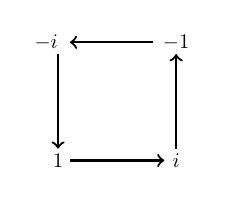
\begin{tikzpicture}[scale=0.75, transform shape]
\draw[->, thick] (0.2,0)--(1.8,0) node at (2,0) {$i$};
\draw[->, thick] (2,0.2)--(2,1.8) node at (2,2) {$-1$};
\draw[->, thick] (1.6,2)--(0.2,2) node at (-0.2,2) {$-i$};
\draw[->, thick] (0,1.8)--(0,0.2) node at (0,0) {$1$};
\end{tikzpicture}
\end{figure}
Отже, ми маємо таку підгрупу:
\begin{align*}
\left<i\right> = \{1,i,-1,-i\}.
\end{align*}
\end{example}

\begin{remark}
Із нескінченної (\textit{нециклічної}) групи ми знайшли скінченну (\textit{циклічну}) підгрупу.
\end{remark}

\begin{example}
Маємо групу $\left< \mathbb{Z}, + \right>$. Всі можливі циклічні підгрупи записані ось таким чином:
\begin{align*}
[k] = [-k] = \{-2k,-k,0,k,2k,\dots\} \overset{\text{позн}}{=} k\mathbb{Z}.
\end{align*}
\end{example}

\begin{example}
Зауважимо, що $\left<1\right> = \mathbb{Z}$, що доводить, що $\left< \mathbb{Z}, + \right>$ буде циклічною групою.
\end{example}

\begin{remark}
Різниця між першими двома прикладами полягала в тому, що:
\begin{itemize}[nosep]
\item в першій циклічній підгрупі рано чи пізно ми знайшли якийсь інший номер $n \in \mathbb{N}$, для якого $a^n = e$ \textit{(у нашому випадку, $i^4 = 1$)};
\item в других циклічних підгрупах ми ніколи не знайдемо $n \in \mathbb{N}$, щоб $a^n = e$.
\end{itemize}
\end{remark}

\begin{definition}
Нехай $\left<G,* \right>$ --- група. Зафіксуємо $a \in G$.\\
\textbf{Порядком елемента} $a \in G$ називають таке найменше число $n$, для якого
\begin{align*}
a^n = e.
\end{align*}
\textit{Позначення}: $\ord (a)$ або $|a|$. \\
Якщо такого порядку не існує, то тоді покладемо $\ord (a) = \infty$.\\
\textbf{Порядком групи $G$} називають просто її потужність:
\begin{align*}
|G| = \card(G).
\end{align*}
\end{definition}

\begin{example}
Зокрема на основі попередніх прикладів:
\begin{enumerate}[nosep,wide=0pt,label={\arabic*)}]
\item для групи $\left< \mathbb{C} \setminus \{0\},\ \cdot \right>$ маємо $\ord(i) = 4$;
\item для групи $\left< \mathbb{Z},+\right>$ маємо $\ord(1) = \infty$.
\end{enumerate}
\end{example}

\begin{lemma}
Нехай $\left< G,* \right>$ --- група та $m = \ord (g)$. Тоді 
\begin{align*}
g^n = e \iff m \mid n.
\end{align*}
\textit{Без доведення. (така ж лема була в теорії чисел під час розмови про первісні корені)}\\
(TODO: а може, прив'язати теорію чисел з теорією груп?)
\end{lemma}

\begin{proposition}
\label{order_of_a_group_is_the_order_of_a_cyclic_subgroup}
Нехай $\left<G,* \right>$ --- група та $\left<a\right>$ --- циклічна підгрупа. Тоді $\ord (a) = |\left<a\right>|$. \\ \textit{(тобто порядок елемента $a$ дорівнює порядку циклічної підгрупи $\left<a\right>$)}
\end{proposition}

\begin{proof}
\begin{enumerate}[topsep=0pt,wide=0pt,label={\Roman*.}]
\item \textit{$\ord(a)$ --- скінченний}.\\
Для зручності позначимо $\ord(a) = n$, тобто зараз маємо $a^n = e$. Отже, циклічна група матиме вигляд:
\[
\left<a\right> = \{e,a,a^2,\dots,a^{n-1}\}.
\]
Залишилося переконатися, що всі зазначені елементи тут справді різні.\\
!Припустимо, що $a^{k_1} = a^{k_2}$ при $0 \leq k_1,k_2 < n$ (\textit{не втрачаючи загальності, нехай $k_1 < k_2$}). У такому разі одержимо, що
\[
a^{k_2-k_1} = e \implies n \mid k_2-k_1 \implies k_2-k_1 \equiv 0 \pmod n.
\]
Однак така рівність можлива лише при $k_2 - k_1 = 0$, тобто отримали $k_2 = k_1$ --- суперечність!\\
Значить, в групі $\left<a\right>$ нема зайвих елементів, а тому $|\left<a\right>| = n$.

\item \textit{$\ord(a)$ --- нескінченний}.\\
Зараз уже маємо, що $a^n \neq e$ для кожного $n \in \mathbb{N}$. Отже, циклічна група матиме вигляд:
\[
\left<a\right> = \{ e,a,a^2,\dots \}
\]
Залишилося переконатися, що всі зазначені елементи тут справді різні.\\
!Припустимо, що $a^{k_1} = a^{k_2}$ при $k_1 \neq k_2$, але тоді
\[ 
a^{k_1-k_2} = e \implies k_1-k_2 = 0 \implies k_1 = k_2.
\]
Одержали суперечність!\\
Значить, в групі $\left<a\right>$ нема зайвих елементів, а тому $|\left<a\right>|$ теж нескінченний. \qedhere
\end{enumerate}
\end{proof}

\begin{remark}
Справедливе наступне:
\begin{align*}
\ord(a) = 1 \iff \left<a\right> = \{e\}.
\end{align*}
\end{remark}

\begin{example}
Розглянемо групу $\left< U_9, \cdot \right>$ та циклічну підгрупу $\left<\overline{2}\right> = \{ \overline{2}, \overline{4}, \overline{8}, \overline{7}, \overline{5} \} = U_9$. Тоді $\ord (\overline{2}) = 5$. (\textit{якщо хтось вчив теорію чисел, то можна зауважити: $2$ --- первісний корінь $\pmod 9$, тому породжує всю групу})
\end{example}

\begin{theorem}
Нехай $\left<G, *\right>$ --- група та $a \in G$, причому $\ord (a) = n$. Тоді для довільного $m \in \mathbb{N}$
\begin{align*}
\left<a^m\right> = \left<a^{\gcd(m,n)}\right>.
\end{align*}
\end{theorem}

\begin{proof}
Нехай $x \in \left<a^m\right>$, тобто $x = (a^m)^k = a^{mk}$. Водночас $\gcd(m,n) = d$, тобто $d \mid m \implies m = dq$. Отже,\[
x = a^{dqk} = (a^d)^{qk} \implies x \in \left<a^{d}\right>.
\]
Нехай $x \in \left<a^d\right>$, тоді $x = (a^d)^k$. За рівністю Безу \[ 
\gcd(m,n) = d = mx + ny,
\] тому отримуємо такий ланцюг:
\[
x= (a^d)^k = a^{dk} = a^{mkx + nky} = (a^{m})^{kx} (a^{n})^{ky} = (a^m)^{kx} \implies x \in \left<a^m\right>. 
\]
Отже, $\left<a^m\right> = \left<a^{\gcd(m,n)}\right>$.
\end{proof}

\begin{example}
Маємо групу $\left< D_{8}, \circ \right>$, де цілком зрозуміло, що $\ord (r) = 8$. За щойно доведеною теоремою 
\[
\left<r^6\right> = \left<r^{\gcd(8,6)}\right> = \left<r^2\right> = \{e,r^2,r^4,r^6\}.
\]
(\textit{попередня теорема просто потрібна, щоб розглядати більш просту підгрупу за виглядом, хоча вони є однаковими}).
\end{example}

\begin{theorem}
Нехай $\left< G, *\right>$ --- циклічна група. Тоді будь-яка підгрупа $H$ --- також циклічна.
\end{theorem}

\begin{proof}
Маємо $G = \left<g\right>$ та $H$ --- деяка підгрупа. Розглянемо два можливих випадки.
\begin{enumerate}[wide=0pt,label={\Roman*.}]
\item \textit{$H$ --- тривіальна підгрупа або $H$ --- невласна}. \\
Тоді або $H = \{e\} = \left<e\right>$, або $H = G = \left<g\right>$ --- тут все автоматично.

\item \textit{$H$ --- нетривіальна власна підгрупа}.\\
Нехай $m \in \mathbb{N}$ --- найменше число, для якого $g^m \neq e$. Хочемо довести, що
\[
H = \left< g^m \right>.
\]
Спочатку скажу, що таке число $m$ існує, бо оскільки $H \neq \{e\}$, то він має містити якийсь елемент $g^m$, де тут може бути або додатний, або від'ємний степінь. Якщо $m > 0$, то оберемо найменше таке число (\textit{well-ordering principle}). Якщо $m < 0$, то тоді обов'язково існує $g^{-m} \in H$, оскільки $H$ --- підгрупа.
\bigskip \\
Тепер доведемо бажану мрію. Нехай $h \in H \subset G$, тоді $h = g^n$ для деякого $n \in \mathbb{Z}$. Поділимо $n$ та $m$:
\begin{align*}
n = mq + r \text{ при } 0 \leq r < m;\\
h = g^n = g^{mq+r} = (g^m)^q g^r.
\end{align*}
Отже, $g^r = (g^m)^{-q} \cdot h$. Зауважимо, що $g^m \in H \implies (g^m)^{-q} \in H$, а також $h \in H$. Таким чином, елемент $g^r \in H$. Але тоді $r \geq m$, бо ми домовились, що $m$ --- найменший степінь для того, щоб $g^m \in H$. А тому вимагаємо $r = 0$. Тобто \[
h = g^n = g^{mq} = (g^m)^q \implies h \in \left<g^m\right>. 
\]
Нехай $h \in \left<g^m\right>$, ну тоді звідси $h = (g^m)^k \in H$, бо $g^m \in H$.
Разом отримали $H = \left<g^m\right>$. \qedhere
\end{enumerate}
\end{proof}

\begin{proposition}
\label{ord_g_to_some_power}
Нехай $\left< G, * \right> = \left<g\right>$ --- циклічна група, $\ord (g) = n$. Тоді при $m < n$ маємо
\begin{align*}
\ord (g^m) =  \dfrac{n}{\gcd(m,n)}.
\end{align*}
\textit{Без доведення. (аналогічна причина)}
\end{proposition}

\begin{example}
Маємо $\left< \mathbb{Z}_n, + \right>$. Тоді твірними групи $\mathbb{Z}_n$ будуть числа $p$, що взаємно прості з $n$.
\end{example}

\begin{theorem}
\label{from_generated_group_get_subgroup}
Нехай $\left< G, *\right>$ --- циклічна група порядка $n$ та $d \mid n$. Тоді існує єдина підгрупа $H$, для якого $|H| = d$.
\end{theorem}

\begin{proof}
\begin{enumerate}[topsep=0pt,wide=0pt,label={\Roman*.}]
\item \textit{Існування}.\\
Зауважимо, що $\left< g^{\frac{n}{d}} \right>$ має рівно $d$ елементів за \prpref{ord_g_to_some_power}. Знайшли підгрупу $H = \left< g^{\frac{n}{d}} \right>$.

\item \textit{Єдиність}.\\
!Припустимо, що існує якась інша підгрупа $H_1$, для якого $|H_1| = d$. Тоді за \thref{from_generated_group_get_subgroup} \[
H_1 = \left<g^m\right> = \left<g^{\gcd(m,n)}\right>.
\]
Отже, отримуємо \[
d = |H_1| = \left|\left<g^{\gcd(m,n)}\right>\right| = \dfrac{n}{\gcd(m,n)}. 
\]
Але тоді $\gcd(m,n) = \dfrac{n}{d}$, а звідси $H_1 = \left< g^{\frac{n}{d}} \right> = H$. Суперечність! \qedhere
\end{enumerate}
\end{proof}

\begin{corollary}
Нехай $\left< G, *\right>$ --- циклічна група порядка $n$ та число $d \mid n$. Тоді кількість елементів $G$ порядка $d$ дорівнює $\varphi(d)$.
\end{corollary}

\begin{theorem}
Задано перестановку $\sigma \in S_n$, розкладемо на незалежні цикли \[\sigma = \sigma_1 \dots \sigma_k, \] довжини кожного циклів відповідно $a_1,\dots,a_k$. Тоді \[
\ord (\sigma) = \lcm(a_1,\dots,a_k).
\]
\end{theorem}

\begin{proof}
Позначимо $m = \ord(\sigma)$ та $l = \lcm(a_1,\dots,a_k)$. Передусім зауважимо, що $\ord(\sigma_i) = a_i$. Також маємо:
\begin{align*}
l = q_1a_1, \quad \dots, \quad l = q_ka_k; \\
\sigma^l = (\sigma_1 \dots \sigma_k)^l\overset{\text{цикли комутують}}{=} \sigma_1^l \dots \sigma_k^l = \sigma_1^{q_1 a_1} \dots \sigma_k^{q_k a_k} = \varepsilon \implies m \mid l; \\
\varepsilon = \sigma^m = \sigma_1^m \dots \sigma_k^m.
\end{align*}
Маємо все одно незалежні цикли, тобто вони не є між собою взаємно оберненими. А значить, єдиний варіант рівності --- це $\sigma_i^m = \varepsilon \implies a_i \mid m$. Тоді $m$ --- спільне кратне чисел $a_1,\dots,a_k \implies l \mid m$.
\end{proof}

\begin{example}
Зокрема перестановка $\sigma = (13) (254)$ із $S_5$ має $\ord(\sigma) = \lcm(2,3) = 6$.
\end{example}

\subsection{Гомоморфізм груп}
\begin{definition}
Нехай $\left<G_1, * \right>$ та $\left<G_2, \star \right>$ --- групи.\\
\textbf{Гомоморфізмом}\footnote{Гомоморфізм перекладається як "одна форма". По суті кажучи, гомоморфізм --- це функція, яка зберігає структуру групи.\\
Ми маємо $a,b \in G_1$, тоді згідно з групою, $a*b \in G_1$. А далі маємо відображення $f \colon G_1 \to G_2$, куди ми переводимось в іншу групу, з іншою операцією. Ці три елементи можна засунути в відображення та отримати $f(a), f(b) \in G_2$, а також $f(a*b) \in G_2$. Ясно, що $f(a) \star f(b) \in G_2$, але додатково хотілось б, щоб це збігалось з $f(a*b)$.} називають відображення $f \colon G_1 \to G_2$, для якого
\begin{align*}
\forall a,b \in G_1: f(a*b) = f(a) \star f(b).
\end{align*}
\end{definition}

\begin{example}
Розглянемо кілька прикладів:
\begin{enumerate}[nosep, wide=0pt,label={\arabic*)}]
\item Маємо групи $\left<\mathrm{GL}_n,\cdot \right>$ та $\left<\mathbb{R} \setminus \{0\}, \cdot \right>$. Розглянемо функцію $f \colon \mathrm{GL}_n \to \mathbb{R} \setminus \{0\}$ таким чином:
\[ f(A) = \det A.\]
Якщо взяти $A,B \in \mathrm{GL}_n$, тобто оборотні матриці, то звідси
\[ 
f(AB) = \det (AB) = \det A \det B = f(A) f(B). 
\]
Отже, $f$ задає гомоморфізм груп.

\item Маємо групи $\left<\mathbb{R},+ \right>$ та $\left<S^1, \cdot \right>$, де множина $S^1$ --- набір комплексних чисел, для яких $|z| = 1$. Розглянемо функцію $\varphi \colon \mathbb{R} \to S^1$ таким чином:
\[ 
\varphi(\theta) = e^{i \theta}. 
\]
Якщо взяти кути $\alpha,\beta \in \mathbb{R}$, отримаємо
\begin{align*}
\varphi(\alpha+\beta) = e^{i (\alpha+\beta)} = e^{i \alpha + i \beta} = e^{i\alpha} \cdot e^{i \beta} = \varphi(\alpha) \cdot \varphi(\beta).
\end{align*}
Фактично кажучи, цим гомоморфізмом ми просто обертаємо дійсну числову лінію навколо кола одиничного радіусу.
\begin{figure}[H]
\centering
\begin{tikzpicture}[scale=0.75, transform shape]
\draw[->, thick] (0,0)--(5,0) node[anchor = north] {$\mathbb{R}$};
\fill[red] ({pi/4},0) circle (2pt)  node[black, anchor=north] {$\dfrac{\pi}{4}$};
\end{tikzpicture}
\qquad
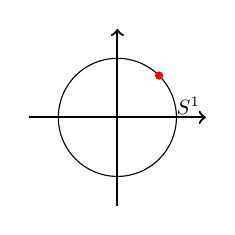
\begin{tikzpicture}[scale=0.75, transform shape]
\draw[->, thick] (-1.5,0)--(1.5,0);
\draw[->, thick] (0,-1.5)--(0,1.5);
\draw (0,0) circle (1);
\node at (1.2,0.2) {$S^1$};
\fill[red] ({cos(45)},{sin(45)}) circle (2pt);
\end{tikzpicture}
\end{figure}
\end{enumerate}
\end{example}

\begin{proposition}[Категорія гомоморфізмів груп\footnote{Для допитливих існує такий розділ математики як теорія категорії. Якщо коротко, \textbf{категорія} $\mathcal{C}$ складається із об'єктів (\textit{у нашому випадку це групи}) та морфізмів між об'єктами (\textit{у нашому випадку це гомоморфізми між групами}), на якій має існувати композиція між морфізмами для кожних об'єктів. Причому композиція має задовольняти асоціативність та існування одиничного морфізму (\textit{у нашому випадку тотожне відображення є гомоморфізмом}) так, щоб при композиції з іншим морфізмом був той же самий морфізм. Коротше, дане твердження каже, що можемо створити категорію та назвати її \textbf{Grp}.}]
Нехай $\left< G, * \right>, \left< H, \star \right>, \left<K, \cdot \right>$ --- групи. Тоді:
\begin{enumerate}[nosep,wide=0pt,label={\arabic*)}]
\item $\id \colon G \to G$ --- гомоморфізм;
\item Якщо $\varphi \colon G \! \to H, \psi \colon H \! \to K$ --- гомоморфізми, то $\psi \circ \varphi \colon G \! \to K$ --- також гомоморфізм;
\item Операція композиції гомоморфізми груп --- асоціативна.
\end{enumerate}
\end{proposition}

\begin{proof}
\begin{enumerate}[topsep=0pt,wide=0pt,label={\arabic*)}]
\item Тут все зрозуміло, але залишу ланцюг:
\[
\id(a*b) = a*b = \id(a)*\id(b).
\]

\item Нехай $a,b \in G$, тоді справедливий такий ланцюг:
\begin{align*}
\psi \circ \varphi(a*b) & = \psi(\varphi(a*b)) \overset{\varphi \text{ --- гомоморфізм}}{=} \psi(\varphi(a) \star \varphi(b)) \overset{\psi \text{ --- гомоморфізм}}{=} \psi(\varphi(a)) \cdot \psi(\varphi(b)) \\ & = \psi \circ \varphi(a) \cdot \psi \circ \varphi(b).
\end{align*}
Отже, $\psi \circ \varphi$ дійсно задає гомоморфізм.
\item (\textit{будь-які відображення між множинами асоціативні}). \qedhere
\end{enumerate}
\end{proof}

\begin{theorem}[Властивості гомоморфізма]
Нехай $\left<G_1, * \right>$ та $\left<G_2, \star \right>$ --- групи з нейтральними елементами $e_1,e_2$ та $f \colon G_1 \to G_2$ --- гомоморфізм груп. Тоді:
\begin{enumerate}[nosep,wide=0pt,label={\arabic*)}]
\item $f(e_1) = e_2$;
\item $\forall a \in G_1: f(a^{-1}) = (f(a))^{-1}$;
\item $\ord (f(g)) \mid \ord (g)$ (\textit{за умови, що $\ord (g)$ --- скінченний});
\item Нехай $H$ --- підгрупа $\left<G_1,*\right>$. Тоді $f(H)$ --- підгрупа $\left<G_2, \star \right>$;
\item Нехай $K$ --- підгрупа $\left<G_2, \star \right>$. Тоді $f^{-1}(K)$ --- підгрупа $\left<G_1,*\right>$.
\end{enumerate}
\end{theorem}

\begin{proof}
\begin{enumerate}[topsep=0pt,wide=0pt, label={\arabic*)}]
\item Тут лише треба згадати правило скорочення, яке виконується в кожних групах:
\[ f(e_1) \star e_2 = f(e_1) = f(e_1*e_1) = f(e_1) \star f(e_1) \overset{\text{скорочення}}{\implies} e_2 = f(e_1). \] 

\item Випливає з цього ланцюга:
\[ f(e_1) = f(a*a^{-1}) = f(a) \star f(a^{-1}) = e_2 \implies f(a^{-1}) = (f(a))^{-1}.
\]

\item Позначимо $\ord(g) = n$, тобто $g^n = e_1$. Тоді $f(g^n) = (f(g))^n$, але тоді звідси $e_2 = f(e_1) = (f(g))^n$, тобто $\ord (f(g)) \mid n = \ord (g)$.

\item Маємо $x,y \in f(H)$, тобто $x = f(a), y = f(b)$ при деяких $a,b \in H$. Тоді \[
x \star y^{-1} = f(a) \star (f(b))^{-1} = f(a) \star f(b^{-1}) = f(a*b^{-1}),
\] причому $a*b^{-1} \in H$. Отже, $x \star y^{-1} \in H$.

\item Маємо $a,b \in f^{-1}(K)$, тобто $f(a),f(b) \in K$, а тому звідси \[
f(a) \star (f(b))^{-1} = f(a * b^{-1}) \in K,
\] тобто $a*b^{-1} \in f^{-1}(K)$. \qedhere
\end{enumerate}
\end{proof}

\begin{definition}
Нехай $\left<G_1, * \right>, \left<G_2, \star \right>$ --- групи та $f \colon G_1 \to G_2$ --- гомоморфізм.\\
Відображення $f$ називається \textbf{ізоморфізмом}, якщо
\begin{align*}
f \text{ --- бієктивне}.
\end{align*}
У такому разі групи $G_1,G_2$ є \textbf{ізоморфними}.\\
\textit{Позначення}: $\left<G_1, * \right> \cong \left<G_2, \star \right>$ або часто пишуть $G_1 \cong G_2$, якщо ясно, які операції сховані.
\end{definition}

\begin{example}
Маємо групи $\left<\mathbb{Z}_2,+ \right>$ та $\left< \{-1,1\},\ \cdot \right>$. Розглянемо відображення \[ 
f \colon \mathbb{Z}_2 \to \{-1,1\}, \qquad f(\overline{0}) = 1,\ f(\overline{1}) = -1.
\]
Ясно, що воно є гомоморфізмом, а також зрозуміло, що кожному елементу з $\{-1,1\}$ ставиться у відповідність єдиний об'єкт з $\mathbb{Z}_2$.  Тобто $f$ --- ізоморфізм, а значить, $\left<\mathbb{Z}_2,+ \right> \cong \left<\{-1,1\},\ \cdot \right>$.
\end{example}

\begin{theorem}[Властивості ізоморфізма]
Нехай $\left<G_1, *\right>, \left<G_2, \star \right>$ --- групи з нейтральними елементами $e_1,e_2$. Нехай $f \colon G_1 \to G_2$ --- ізоморфізм. Тоді:
\begin{enumerate}[nosep,wide=0pt,label={\arabic*)}]
\item $f^{-1} \colon G_2 \to G_1$ --- також ізоморфізм;
\item $\left< G_1, * \right>$ --- абелева (циклічна) $\iff \left< G_2, \star \right>$ --- абелева (циклічна);
\item $\ord(g) = \ord(f(g))$.
\end{enumerate}
\end{theorem}

\begin{proof}
\begin{enumerate}[topsep=0pt,wide=0pt,label={\arabic*)}]
\item $f$ --- ізоморфізм, тобто бієктивний гомоморфізм, тоді $f^{-1}$ --- також бієктивне відображення. Залишилось довести, що теж гомоморфізм. Для кожних $x,y \in G_2$ маємо:
\[
f^{-1}(x \star y) = f^{-1}(f(f^{-1}(x)) \star f(f^{-1}(y)))  = f^{-1}(f(f^{-1}(x)*f^{-1}(y))) = f^{-1}(x)*f^{-1}(y).
\]

\item Нехай $G_1$ --- абелева. Тоді для кожних $x,y \in G_2$ маємо:
\[
x \star y = f(f^{-1}(x)) \star f(f^{-1}(y)) = f(f^{-1}(x) * f^{-1}(y)) = f(f^{-1}(y) * f^{-1}(x)) = f(f^{-1}(y)) \star f(f^{-1}(x)) = y \star x.
\]
Нехай $G_1$ --- циклічна, тобто $G_1 = \left<g\right>$. Маємо $x \in G_2$, тоді $x = f(a)$ за сюр'єктивністю. Але $a \in G_1$, тоді звідси $a = g^n$, а тому $x = f(g^n)) = (f(g))^n$. Отже, $G_2 \subset \left<f(g)\right>$. Ясно, що $\left<f(g)\right> \subset G_2$, а тому $G_2 = \left<f(g)\right>$ --- циклічна.\\
Із того, що $G_2$ абелева (циклічна) аналогічно випливає, що $G_1$ --- абелева (циклічна).

\item Оскільки $f$ --- гомоморфізм, то $\ord(f(g)) \mid \ord(g)$. Водночас $\ord(g) = \ord(f^{-1}(f(g)) \mid \ord(f(g))$, тому що $f^{-1}$ --- гомоморфізм. Отже, $\ord(g) = \ord(f(g))$. \qedhere
\end{enumerate}
\end{proof}

\begin{theorem}
Нехай $\left<G,* \right>$ --- група, $\left<a\right>$ --- циклічна підгрупа, $a \in G$, а також $\ord(a) = n \in \mathbb{N}$. Тоді 
\begin{align*}
\left<\left<a\right>, *\right> \cong \left< \mathbb{Z}_n, + \right>.
\end{align*}
\end{theorem}

\begin{proof}
Побудуємо функцію 
\[ 
f \colon \mathbb{Z}_n \to \left<a\right>,\qquad f(\overline{k}) = a^k,
\] 
де число $k = 0,\dots,n-1$.
\begin{enumerate}[wide=0pt,label={\Roman*.}]
\item \textit{$f$ --- гомоморфізм}.\\
Дійсно, нехай $\overline{k}, \overline{m} \in \mathbb{Z}_n$. Тоді
\[
f(\overline{k}+\overline{m}) = f(\overline{k+m}) = a^{k+m} = a^k * a^m = f(\overline{k})*f(\overline{m}).
\]

\item \textit{$f$ --- бієктивне}.\\
Сюр'єкція ясно, що виконана. Ін'єкція виконана, бо 
\[
f(\overline{k}) = f(\overline{m}) \implies a^k = a^m \implies k = m,
\] 
це було доведено в доведенні \prpref{order_of_a_group_is_the_order_of_a_cyclic_subgroup}. 
\end{enumerate}
Отже, $f$ --- ізоморфізм та $\left<\left<a\right>, *\right> \cong \left< \mathbb{Z}_n, + \right>$.
\end{proof}

\begin{theorem}
Нехай $\left<G,* \right>$ --- група, $\left<a\right>$ --- циклічна підгрупа, $a \in G$, а також $\ord(a) = \infty$. Тоді 
\[
\left<\left<a\right>, *\right> \cong \left< \mathbb{Z}, + \right>.
\]
\end{theorem}

\begin{proof}
Побудуємо функцію 
\[
f \colon \mathbb{Z} \to \left<a\right>, \qquad f(k) = a^k.
\]
А далі все майже аналогічно, як в попередній теоремі.
\end{proof}

\begin{example}
Зокрема група $S_n$ --- не циклічна.
\bigskip \\
!Припустимо, що $S_n = \left<\sigma\right>$, тобто циклічна. Тоді $S_n \cong \mathbb{Z}_{n!}$. Тобто задається ізоморфізм, а значить за властивістю 2) оскільки $\mathbb{Z}_{n!}$ --- абелева, то тоді $S_n$ --- абелева теж --- це суперечність!
\end{example}

\begin{example}
Знайти всі гомоморфізми $f \colon \mathbb{Z}_8 \to \mathbb{Z}_{12}$.
\bigskip \\
Зауважимо, що якщо $f$ --- гомоморфізм, то $f(\overline{k}) = k f(\overline{1})$ при $k = 0,1,\dots,7$. Тобто нам достатньо зрозуміти, чому може дорівнювати $f(\overline{1})$, тим самим визначиться гомоморфізм.\\
Маємо $f(\overline{8}) = 8 f(\overline{1}) = f(\overline{0}) = \overline{0}$. Таким чином, 
\[8 f(\overline{1}) \equiv 0 \pmod{12}.\]
Розв'язавши конгруентне рівняння, отримаємо $f(\overline{1}) \in \{ 0,3,6,9 \}$. Отже, знайшли $4$ гомоморфізми:
\begin{align*}
f_1(\overline{k}) = \overline{0},\ f_2(\overline{k}) = 3\overline{k},\ f_3(\overline{k}) = 6 \overline{k},\ f_4(\overline{k}) = 9 \overline{k}.
\end{align*}
\end{example}

\subsubsection*{Інший спосіб записати означення підгрупи}
\begin{proposition}
Нехай $\left< G,*\right>$ --- група та $H \subset G$. Нехай $\left<H,\cdot\right>$ --- група (\textit{поки що ми вважаємо, що в нього якась інша операція}). Тоді
\begin{center}
$H$ --- підгрупа $G \iff \imath \colon H \hookrightarrow G$ задає гомоморфізм груп.
\end{center}
\end{proposition}

\begin{proof}
\rightproof Дано: $H$ --- підгрупа $G$, тобто, насправді, $\cdot \equiv *$ (\textit{людською мовою операція на $H$ така ж, що в й групі $G$}). Нехай $h_1,h_2 \in H$. Тоді 
\[
\imath (h_1 * h_2) = h_1 * h_2 = \imath(h_1) * \imath(h_2).
\]
\leftproof Дано: $\imath \colon H \to G$ задає гомоморфізм. Тобто для будь-яких $h_1,h_2 \in H$
\[
h_1 \cdot h_2 = \imath(h_1 \cdot h_2) = \imath(h_1) * \imath(h_2) = h_1 * h_2. \]
Із точки зору бінарного відображення, ми довели, що $\cdot \equiv *|_H$. Таким чином, $H$ --- підгрупа $G$ (\textit{бо успадкувала операцію}).
\end{proof}

% Alternative but harder version of Cayley's theorem
\iffalse
\subsubsection*{Ще трошки про групу перестановок}

\begin{theorem}[Теорема Келі]
Нехай $\left< G,*\right>$ -- група. Тоді існує підгрупа перестановок $H \subset S_G$, для якої $\left< G, *\right> \cong \left< H, \circ \right>$.
\end{theorem}

\begin{proof}
Маємо $g \in G$, визначимо відображення $\lambda_g \colon G \to G$ таким чином: $\lambda_g(x) = g*x$. Покажемо, що $\lambda_g \in S_G$, що теж саме, що воно бієктивне.\\
$\lambda_g(x) = \lambda_g(y) \implies g*x = g*y \implies x = y$ -- ін'єктивність є.\\
$\forall y \in G: \exists x = g^{-1}*y \in G: \lambda_g(x) = \lambda_g(g^{-1}*y) = g*(g^{-1}*y) = y$ -- сюр'єктивність є.
\bigskip \\
Встановимо множину $H = \{ \lambda_g \mid g \in G\}$, причому $H \subset S_G$. Покажемо, що це -- підгрупа $\left< S_G, \circ \right>$.\\
Асоціативність ясно, що виконується.\\
$\lambda_e(x) = e*x = x$ -- нейтральний елемент -- ясно.\\
$\forall \lambda_g: \exists \lambda_{g^{-1}}: \lambda_g \circ \lambda_{g^{-1}} (x) = \lambda_g(g^{-1}*x) = g*(g^{-1}*x) = x = \lambda_e(x)$ -- оберненість є.
\bigskip \\
Нарешті, покажемо, що $G \cong H$, для цього треба встановити $\varphi \colon G \to H$ так, що $\varphi(g) = \lambda_g$. Це буде гомоморфізмом, бо\\
$\varphi(g*h) = \lambda_{g*h}$, але $\lambda_{g*h}(x) = (g*h)*x = g*(h*x) = \lambda_g(h*x) = \lambda_g \circ \lambda_h$, тобто $\varphi(g*h) = \varphi(g) \circ \varphi(h)$.\\
Ін'єкція та сюр'єкція над $\varphi$ ясно, що виконується. Отже, $G \cong H$.
\end{proof}
\fi

%wrong statement
\iffalse
\begin{corollary}
Задано $\left< G, * \right>$ -- група з $\ord G = n$. Тоді $\left< G,*\right> \cong \left< S_n, \circ \right>$.
\end{corollary}
\fi

Нехай $\left< G, * \right>, \left< H, \cdot \right>$ --- групи.\\
\textit{Позначення}: $\homom{G}{H}$ --- множина всіх гомоморфізмів з $G$ в $H$.\\
Установимо для неї операцію 
\[
(f \cdot g)(x) = f(x) \cdot g(x),\ \forall x \in G.
\]
Загалом $\left< \homom{G}{H}, \cdot \right>$ не задає групу. Дійсно, нехай $f,g,h \in \homom{G}{H}$, тоді:
\begin{align*}
(f \cdot g)(x_1 * x_2) = f(x_1 * x_2) \cdot g(x_1 * x_2) = (f(x_1) \cdot f(x_2)) \cdot (g(x_1) \cdot g(x_2)). \\
(f \cdot g)(x_1) \cdot (f \cdot g)(x_2) = f(x_1) \cdot g(x_1) \cdot f(x_2) \cdot g(x_2).
\end{align*}
Тобто ми таким чином показали, що $f \cdot g$ не обов'язково може бути гомоморфізмом, тобто $f \cdot g \notin \homom{G}{H}$ --- порушується замкненість.
\bigskip \\
Утім якщо попросити групу $\left< H,\cdot \right>$ бути абелевою, то тоді замкненість вже буде працювати. Гомоморфізми між собою асоціативні. Нейтральний елемент --- це гомоморфізм $\sigma \colon G \to H$, що задається як $\sigma(g) = e_H$. Для кожного гомоморфізму $f \colon G \to H$ його оберненим буде гомоморфізм $g \colon G \to H$, що задається як $g(x) = (f(x))^{-1}$.


%Later
\iffalse
\subsection{Ендоморфізми та автоморфізми}
\begin{definition}
Задано $\left< G, * \right>$ -- група.\\
Гомоморфізм $f$ є \textbf{ендоморфізмом}, якщо в нас таке відображення:
\begin{align*}
f \colon G \to G,
\end{align*}
тобто із групи в $G$ на ту саму групу $G$.\\
Позначення: $\End{G}$ -- множина всіх ендоморфізмів.
\end{definition}

\begin{definition}
Задано $\left< G, * \right>$ -- група.\\
Відображення $f$ називається \textbf{автоморфізмом}, якщо
\begin{align*}
f \colon G \to G \text{ -- ізоморфізм}
\end{align*}
Позначення: $\Aut{G}$ -- множина всіх автоморфізмів.
\end{definition}

\begin{remark}
$\End{G} = \homom{G}{G}$ \qquad $\Aut{G} \subset \End{G}$.
\end{remark}
\fi

\subsection{Ядра, образи гомоморфізмів}
\begin{definition}
Нехай $\left<G_1, * \right>,\left<G_2, \star \right>$ --- групи та $f \colon G_1 \to G_2$ --- гомоморфізм.\\
\textbf{Ядром} гомоморфізма називають множину
\begin{align*}
\ker f = \{ x \in G_1: f(x) = e_2 \}.
\end{align*}
\textbf{Образом} гомоморфізма називають множину
\begin{align*}
\Im f = \{f(x) : x \in G_1\}.
\end{align*}
\end{definition}

\begin{remark}
Компактно кажучи, $\ker f = f^{-1}(\{e_2\})$, а також $\Im f = f(G_1)$.
\bigskip \\
Таким чином, оскільки $\{e_2\},\ G_1$ є підгрупами для свої груп, то за властивостями гомоморфізма $f^{-1}(\{e_2\}),\ f(G_1)$ будуть підгрупами для своїх груп як прообраз та образ відповідно.
\end{remark}

\begin{example}
Розглянемо групи $\left<\mathbb{R},+\right>,\ \left<S^1,\cdot \right>$ та гомоморфізм 
\[
\varphi(\theta) = \cos \theta + i \sin \theta \overset{\text{або}}{=} e^{i\theta}. 
\]
Знайдемо $\ker \varphi$ та $\Im \varphi$. Зауважу заздалегідь, що ми маємо нейтральні елементи $0 \in \mathbb{R}$ та $1 \in S^1$.
\[
\theta \in \ker \varphi \iff \varphi(\theta) = e^{i \theta} = 1 \iff \theta = 2 \pi k, k \in \mathbb{Z}.
\]
Отже, ми одержали, що
\[
\ker \varphi = \{2 \pi k \mid k \in \mathbb{Z}\}.
\]
Нехай $z \in S^1$, тобто $|z| = 1$, а також як комплексне число $z = \cos \theta + i \sin \theta = \varphi(\theta)$ при деякому $\theta \in \mathbb{R}$, звідси $z \in \Im \varphi$. Із урахуванням того, що $\Im \varphi \subset S^1$, ми отримаємо
\[ 
\Im \varphi = S^1.
\]
\end{example}

\begin{theorem}
Нехай $\left<G_1, * \right>,\ \left<G_2, \star \right>$ --- групи та $f \colon G_1 \to G_2$ --- гомоморфізм. Тоді
\begin{center}
$f$ --- ін'єктивний\footnote{Інколи ін'єктивний гомоморфізм називають \textbf{мономорфізмом}. Насправді, в теорії категорії розрізняють ін'єктивний морфізм та мономорфізм та не завжди є одними й тими самими речами. Однак в категорії \textbf{Grp} ці два поняття збігаються.} $\iff \ker f = \{e_1\}$.
\end{center}
\end{theorem}

\begin{proof}
\rightproof Дано: $f$ --- ін'єктивний гомоморфізм. Маємо $x \in \ker f$, тоді одержимо ось такий ланцюг:
\[
f(x) = e_2 \implies f(x) = f(e_1) \overset{f \text{ --- ін'єктивний}}{\implies} x = e_1.
\]
Отже, одержали $\ker f = \{e_1\}$.
\bigskip \\
\leftproof Дано: $\ker f = \{e_1\}$.\\
!Припустимо, що $f$ --- не ін'єктивне, тобто при $x_1 \neq x_2$ отримаємо $f(x_1) = f(x_2)$. Тоді
\[ f(x_1)\star(f(x_2))^{-1} = f(x_1) \star f(x_2^{-1}) = f(x_1 * x_2^{-1}) = e_2.
\]
Це означає, що $x_1*x_2^{-1} \in \ker f$, тому 
\[
x_1*x_2^{-1} = e_1 \implies x_1 = x_2.
\]
Отримали суперечність!
\end{proof}

\begin{example}
Гомоморфізм $\varphi \colon \mathbb{R} \to S^1$ вище не буде ін'єктивним, оскільки $\ker f$ містить інші елементи, окірм нейтрального $0$.
\end{example}

\iffalse
\begin{proposition}[Ще одна властивість гомоморфізма]
Задані $\left<G_1, * \right>,\left<G_2, \star \right>$ -- групи та $f \colon G_1 \to G_2$ -- гомоморфізм. Тоді якщо $N \triangleleft G_2$, то $f^{-1}(N) \triangleleft G_1$.
\end{proposition}

\begin{proof}
Уже доводили, що $f^{-1}(N)$ буде підгрупою $G_1$.\\
Маємо $n \in f^{-1}(N)$ та $g \in G_1$. Тоді $f(n) \in N, f(g) \in G_2$. Оскільки $N$ -- нормальний дільник, то звідси $f(g) \star f(n) \star (f(g))^{-1} = f(g*n*g^{-1}) \in N$, а тому $g*n*g^{-1} \in f^{-1}(N)$.\\
Отже, $f^{-1}(N) \triangleleft G_1$.
\end{proof}

\begin{corollary}
$\ker f \triangleleft G_1$.\\
\textit{Щоправда, за образ так не скажеш.}
\end{corollary}

\begin{example}
Приклад, де $\Im f \centernot\triangleleft G_2$. Розглянемо $\left<H, \cdot \right>$ -- підгрупа всіх нижньотрикутних матриць, причому $H \subset \mathrm{GL}_2$. Маємо гомоморфізм $f \colon H \to H$ заданий таким чином:\\
$f\left( \begin{pmatrix}
a_{11} & 0 \\
a_{21} & a_{22}
\end{pmatrix} \right) = \begin{pmatrix}
a_{11} & 0 \\
0 & a_{22}
\end{pmatrix}$.\\
Беремо $A = \begin{pmatrix}
1 & 0 \\
1 & 1
\end{pmatrix} \in H$ та $A = \begin{pmatrix}
1 & 0 \\
0 & 2
\end{pmatrix} \in \Im f$, тоді\\
$\begin{pmatrix}
1 & 0 \\
1 & 1
\end{pmatrix} \cdot \begin{pmatrix}
1 & 0 \\
0 & 2
\end{pmatrix} \cdot \begin{pmatrix}
1 & 0 \\
1 & 1
\end{pmatrix}^{-1} = \begin{pmatrix}
1 & 0 \\
-1 & 2
\end{pmatrix} \not \in \Im f$.
\end{example}
\fi

\subsection{Суміжні класи}
Нехай $\left< G, *\right>,\ \left< G', \star \right>$ --- групи та $f \colon G \to G'$ --- гомоморфізм. Визначимо цілком очевидне відношення еквівалентності: 
\[
g_1 \sim g_2 \iff f(g_1) = f(g_2).
\]
Окремо пропишемо рівність, помноживши зліва на $(f(g))^{-1}$ --- отримаємо \[
(f(g_1))^{-1} \star f(g_2) = e_{G'} \iff f(g_1^{-1}) \star f(g_2) = e_{G'} \iff f(g_1^{-1}*g_2) = e_{G'} \iff g_1^{-1}*g_2 \in \ker f.
\]
Таким чином, ми одержали
\[
g_1 \sim g_2 \iff g_1^{-1}*g_2 \in \ker f.
\]
Але $\ker f$ --- це один із підгруп $G$. Ми хочемо ці міркування повторити для кожної підгрупи.
\bigskip \\
Нехай $H$ --- підгрупа $G$, встановимо схоже відношення еківалентності (\textit{вправа: довести, що це дійсно задає відношення еквівалентності}):
\[
g_1 \sim g_2 \iff g_1^{-1}*g_2 \in H.
\]
Після цього ми можемо розбити $G$ на класи еквівалентності.

\begin{definition}
\textbf{Лівим суміжним класом $g$ за підгрупою $H$} назвемо клас еквівалентності
\begin{align*}
[g] \overset{\text{позн.}}{=} g*H.
\end{align*}
(\textit{я часто класи еквівалентності позначаю за $[g]$, в теорії груп буде вже своє позначення}).
\end{definition}

Таке позначення виправдане, оскільки маємо ось це:

\begin{proposition}
Лівий суміжний клас класа $g$ за підгрупою $H$ можна записати ось так:
\begin{align*}
g*H = \{ g*h \mid h \in H \}.
\end{align*}
\end{proposition}

\begin{proof}
Нехай $x \in g*H$, тобто звідси $x^{-1}*g \in H$. Але тоді $x = x*(x^{-1}*g)$, причому елемет $x \in G,\ x^{-1}*g \in H$. Тобто $x$ потрапляє в праву множину.\\
Нехай $x$ потрапяє в праву множину, тобто $x = g*h,\ h \in H$. Але тоді $h = g^{-1}*x \in H \implies x^{-1}*g \in H$, тобто $x \sim g$. Звідси $x \in g*H$.
\end{proof}

Фактормножина $G/_{\sim} \overset{\text{позн.}}{=} G/_H$ буде містити всі ліві суміжні класи.

\begin{proposition}
Справедливе наступне:
\begin{align*}
g_1 * H = g_2 * H \iff g_1^{-1}*g_2 \in H.
\end{align*}
\textit{Це випливає з того, що $g_1^{-1}*g_2 \in H \iff g_1 \sim g_2 \iff [g_1] = [g_2] \iff g_1*H = g_2*H$. У такому формулюванні ми будемо часто користуватися.}
\end{proposition}

Повернімося до самого початку, до $g_1 \sim g_2 \iff f(g_1) = f(g_2)$. Праву рівність можна записати іншим способом, помноживши уже справа на $(f(g))^{-1}$ --- отримаємо:
\[
f(g_2) \star (f(g_1))^{-1} = e_{G'} \iff f(g_2) \star f(g_1^{-1}) = e_{G'} \iff f(g_2*g_1^{-1}) \in e_{G'} \iff g_2*g_1^{-1} \in \ker f.\]
Таким чином, ми отримали 
\[
g_1 \sim g_2 \iff g_2*g_1^{-1} \in \ker f.
\]
Тепер для $H$ можна задати інше відношення еквівалентності (\textit{знову вправа: довести}):
\[
g_1 \sim g_2 \iff g_2*g_1^{-1} \in H.
\]
Ми потім знову розіб'ємо $G$ на класи еквівалентності.

\begin{definition}
\textbf{Правим суміжним класом $g$ за підгрупою $H$} назвемо клас еквівалентності
\begin{align*}
[g] \overset{позн.}{=} H*g.
\end{align*}
\end{definition}

\begin{proposition}
Правий суміжний клас класа $g$ за підгрупю $H$ можна записати ось так:
\begin{align*}
H*g = \{ h*g \mid h \in H \}.
\end{align*}
\textit{Аналогічне доведення, як було з лівим суміжним класом.}
\end{proposition}

Фактормножина $G/_{\sim} \overset{\text{позн.}}{=} {}_{H}{/G}$ буде містити всі праві суміжні класи.

\begin{proposition}
Справедливе наступне:
\begin{align*}
H * g_1 = H * g_2 \iff g_2*g_1^{-1} \in H.
\end{align*}
\textit{Аналогічні міркування. Знову цим будемо частіше користуватися.}
\end{proposition}

\begin{example}
\label{trivial_cosets}
Розглянемо тривіальну та невласну підгрупи групи $\left<G,* \right>$. Знайдемо суміжні класи.
\begin{enumerate}[nosep,wide=0pt,label={\arabic*)}]
\item $g*\{e\} = \{e\}*g = \{g\}$, і це виконується для кожного $g \in G$;
\item $g*G = G*g = G$, і це виконується для кожного $g \in G$.
\end{enumerate}
\end{example}

Коли в нас підгрупа $H = \ker f$, то тоді ліві та праві суміжні класи збігалися, тому все чудово. Виникає логічне питання: чи буде так з довільною підгрупою $H$? Відповідь: ні.

\begin{example}
Маємо групу $\left<S_3, \circ \right>$ та підгрупу $H = \{ (23), (1) \} \overset{\text{або}}{=} \left<(23)\right>$. Знайдемо всі можливі як й ліві, так й праві суміжні класи:
\begin{align*}
\begin{tabular}{ll}
$(1) \circ H = \{(23),(1)\}$, & $H \circ (1) = \{(23),(1)\}$;\\
$(23) \circ H = \{(23),(1)\}$, & $H \circ (23) = \{(23),(1)\}$;\\
$(13) \circ H = \{(132),(13)\}$, & $H \circ (13)  = \{(123),(13)\}$;\\
$(12) \circ H = \{(123),(12)\}$, & $H \circ (12)  = \{(132),(12)\}$;\\
$(123) \circ H = \{(123),(12)\}$, & $H \circ (123) = \{(123),(13)\}$;\\
$(132) \circ H = \{(132),(13)\}$, & $H \circ (132) = \{(132),(12)\}$.\\
\end{tabular}
\end{align*}
Уже на цьому прикладі зауважимо, що загалом $g * H \neq H* g$.
\end{example}

За яких умов ці суміжні класи ще збігатимуться, дізнаємося згодом. Зараз кілька важливих наслідків із того, що ми зробили, та корисні твердження.

\begin{corollary}
Ліві суміжні класи між собою або не перетинаються, або збігаються. Так само праві суміжні класи між собою або не перетинаються, або збігаються.\\
\textit{Тому що класи еквівалентності або не перетинаються, або збігаються.}
\end{corollary}

\begin{corollary}
Будь-яка група $\left<G,*\right>$ розбивається таким чином:
\begin{align*}
G = \displaystyle\bigcup_{g \in G} g*H, \qquad G = \displaystyle\bigcup_{g \in G} H*g.
\end{align*}
\textit{Тому що класи еквівалентності утворюють розбиття множини.}
\end{corollary}

\begin{example}
Зокрема за попереднім прикладом маємо:
\begin{align*}
S_3 = \{(23), (1)\} \cup \{(132), (13)\} \cup \{(123), (12)\}, \\
S_3 = \{(23), (1)\} \cup \{(123), (13)\} \cup \{(132), (12)\}.
\end{align*}
Перше --- об'єдняння лівих суміжних класів. Друге --- об'єднаяння правих суміжних класів.
\end{example}

\begin{remark}
Даний наслідок сформульовано окремо для лівих суміжних класів та правих. Мається на увазі, що $a*H$ та $H*b$ можуть мати непорожній перетин.
\bigskip \\
Зокрема з попереднього прикладу, $(13) \circ H \cap H \circ (12) = \{(132)\}$.
\end{remark}

\begin{proposition}
Справедливе наступне:
\begin{align*}
g_1 * H = g_2 * H \iff H * g_2^{-1} = H * g_1^{-1}.
\end{align*}
\end{proposition}

\begin{proof}
\rightproof Дано: $g_1 * H = g_2 * H$.\\
Нехай $x \in H*g_2^{-1}$, тоді $x = h*g_2^{-1}$ для деякого $h \in H$. Оскільки $g_2 \in g_2*H$, то $g_2 \in g_1*H \implies g_2 = g_1*h'$ для деякого $h' \in H$. Отже, $x = h*(h')^{-1}*g_1^{-1}$, що означає $x \in H*g_1^{-1}$.\\
Нехай $x \in H*g_1^{-1}$, тоді аналогічним чином $x \in H*g_2^{-1}$.\\
Висновок: $H*g_2^{-1} = H*g_1^{-1}$.
\bigskip \\
\leftproof \textit{доведення є дзеркальним}.
\end{proof}

\begin{proposition}
\label{card_g_times_H_equals_card_H}
Нехай $\left<G,* \right>$ --- скінченна група та $H \leq G$. Тоді для кожного елемента $g \in G$ виконується 
\begin{align*}
\card(g*H) = \card(H).
\end{align*}
\textit{Для правих суміжних класів аналогічне твердження}.
\end{proposition}

\begin{proof}
Припустимо, що $H = \{h_1,\dots,h_k\}$ --- тут елементи різні. Тоді маємо $g*H = \{g*h_1,g*h_2,\dots,g*h_k\}$.  Єдине, що треба довести, --- це те, що $g*h_i \neq g*h_j$ для кожних $i \neq j$.\\
!Припустимо, що $g*h_i = g*h_j$. Тоді автоматично звідси $h_i = h_j$. Ну але ж ми маємо різні елементи, тому суперечність!\\
Отже, $\text{card}(g*H) = k$.
\end{proof}

\begin{proposition}
Нехай $\left< G, * \right>$ --- скінченна група та $H \leq G$. Тоді кількість лівих суміжних класів збігається з кількістю правих суміжних класів.
\end{proposition}

\begin{proof}
Визначимо множини \[
\mathcal{L}_H = \{g*H \mid g \in G\}, \qquad \mathcal{R}_H = \{H*g \mid g \in G\}.
\]
Визначимо відображення \[
f \colon \mathcal{L}_H \to \mathcal{R}_H, \qquad f(g*H) = H*g^{-1}.
\]
\begin{enumerate}[wide=0pt,label={\Roman*.}]
\item \textit{$f$ --- визначено коректно}.\\
Дійсно, якщо $x*H = y*H$, то 
\[
f(x*H) = H*x^{-1} =H*y^{-1} = f(y*H).
\]
\item \textit{$f$ --- бієктивне}.\\
Ін'єктивність доводиться в один рядок:
\[
f(x*H) = f(y*H) \implies H*x^{-1} = H*y^{-1} \implies x*H = y*H.
\]
Сюр'єктивність також швидко. Якщо $H*g \in \mathcal{R}_H$, то існує $g^{-1}*H \in \mathcal{L}_H$, для якого $f(g^{-1}*H) = H*g$.
\end{enumerate}
Внаслідок чого одержимо, що $\card(\mathcal{L}_H) = \card(\mathcal{R}_H)$.
\end{proof}

\begin{definition}
Нехай $\left< G, * \right>$ --- скінченна група, $H \leq G$.\\
\textbf{Індексом підгрупи $H$ в групі $G$} називають кількість суміжних класів.\\
\textit{Позначення}: $[G:H]$.
\end{definition}

\begin{remark}
Уже доводили, що кількість лівих та правих суміжних класів однакова, тому дане означення має сенс.
\end{remark}

\begin{proposition}
Нехай $\left< G,*\right>$ --- група та $H \leq K \leq G$. Тоді
\begin{align*}
[G:H] = [G:K] \cdot [K:H].
\end{align*}
\end{proposition}

\begin{proof}
Відомо, що
\[
[G:H] \cdot \card(H) = \card(G), \qquad [G:K] \cdot \card(K) = \card(G).
\]
Звідси випливає, що $[G:H] \cdot \card(H) = [G:K] \cdot \card(K)$. Зауважимо, що $H$ можна сприймати як підгрупу $K$ (\textit{не просто як підгрупу $G$}). А всі сужміжні класи $k*H \subset K$, а тому там є розбиття $K$ на об'єднання суміжних класів $k*H$ --- все коректно тоді буде.\\
Маємо ще рівняння \[ 
[K:H] \cdot \card(H) = \card(K).
\] 
Підставивши це вище, отримуємо 
\begin{gather*}
[G:H] = [G:K] \cdot [K:H]. \qedhere
\end{gather*} 
\end{proof}

\begin{theorem}[Теорема Лагранжа]
Нехай $\left<G,* \right>$ --- скінченна група та $H \leq G$. Тоді 
\begin{align*}
\card H \mid  \card G.
\end{align*}
\end{theorem}

\begin{proof}
Припускаємо, що $\card G = m$. Маємо розбиття
\[ 
G = \displaystyle\bigcup_{k=1}^n g_k*H,
\]
де число $n \leq m$. Сюди ми записали лише таку кількість суміжних класів, де вони не співпадають. Оскільки ці множини не перетинаються, то 
\[
\card(G) = \card(g_1*H) + \dots + \card(g_n*H) \overset{\text{\prpref{card_g_times_H_equals_card_H}}}{=} \card(H) + \dots + \card(H) = n \cdot \card(H).
\]
Отже, $\card(H) \mid \card(G)$.
\end{proof}

\begin{corollary}
На основі теореми Лагранжа маємо:
\begin{align*}
\card(G) = [G:H] \cdot \card(H).
\end{align*}
Також можна записати це як
\begin{align*}
\card(G) = \card(G/_H) \cdot \card(H) \quad \text{або} \quad \card(G) = \card({}_{H}{/G}) \cdot \card(H).
\end{align*}
\end{corollary}

\begin{example}
Група $\left<S_3, \circ \right>$ не може містити підгрупи $H$, що складаються з $4$ або $5$ елементів (\textit{випливає безпосередньо з теореми Лагранжа}).
\end{example}

\begin{corollary}[Наслідки з теореми Лагранжа]
Нехай $\left< G,*\right>$ --- скінченна група. Тоді:
\begin{enumerate}[nosep,wide=0pt,label={\arabic*)}]
\item Якщо $\card G = p$, де $p$ --- просте число, то тоді $G$ містить лише тривіальну та невласну підгрупи (\textit{тобто $G$ --- циклічна група});
\item $\ord(a) \mid \card G$ для кожного $a \in G$;
\item $a^{\card G} = e$ для кожного $a \in G$.
\end{enumerate}
\textit{Вправа: довести.}
\end{corollary}

\begin{theorem}[Теорема Ойлера]
Нехай числа $a,n$ --- взаємно прості. Тоді
\begin{align*}
a^{\varphi(n)} \equiv 1 \pmod n.
\end{align*}
\textit{У теорії чисел це доводилось, але наведемо інший спосіб.}
\end{theorem}

\begin{proof}
Маємо скінченну групу $\left<U_n,\cdot\right>$, причому $\card(U_n) = \varphi(n)$ за визначенням функції Ойлера. Тоді за наслідком теореми Лагранжа, 
\[
\overline{a}^{\card(U_n)} = \overline{a}^{\varphi(n)} = \overline{a^{\varphi(n)}} = \overline{1}.
\]
Отже, $a^{\varphi(n)} \equiv 1 \pmod n$.
\end{proof}

\subsection{Нормальні підгрупи}
\begin{definition}
Нехай $\left<G,* \right>$ --- група та $H \leq G$.\\
Підгрупа $H$ називається \textbf{нормальною} (або \textbf{нормальним дільником}), якщо:
\begin{align*}
\forall g \in G: g*H = H*g.
\end{align*}
\textit{Позначення}: $H \triangleleft G$.
\end{definition}

\begin{remark}
Еквівалентне означення звучатиме ось так:
\begin{align*}
\forall g \in G: H = g*H*g^{-1}.
\end{align*}
\end{remark}

\begin{example}
Якщо $\left<G,* \right>$ --- абелева група, то будь-яка підгрупа $H \triangleleft G$.
\end{example}

\begin{example}
Для будь-якої групи $\left<G,*\right>$ маємо $\{e\} \triangleleft G$ та $G \triangleleft G$ (див.~ \exref{trivial_cosets}).
\end{example}

\begin{example}
Маємо групу $\left<S_3, \circ \right>$ та підгрупу $H = \{(123),(132),(1)\} \overset{\text{або}}{=} \left<(123)\right>$. Тоді
\begin{align*}
(1) \circ H = H \circ (1) = \{(123),(132),(1)\}, \\
(23) \circ H = H \circ (23) = \{(23),(13),(12)\}, \\
(13) \circ H = H \circ (13) = \{(23),(13),(12)\}, \\
(12) \circ H = H \circ (12) = \{(23),(13),(12)\}, \\
(123) \circ H = H \circ \varphi_1 = \{(123),(132),(1)\}, \\
(132) \circ H = H \circ \varphi_2 = \{(123),(132),(1)\}.
\end{align*}
Таким чином, $\{(123),(132),(1)\} \triangleleft S_3$.
\end{example}

\iffalse
\begin{remark}
Довільна група може мати й нормальні, так й ненормальні (ору, ненормальні) підгрупи.
\end{remark}
\fi

\begin{theorem}[Критерій нормальної підгрупи]
Нехай $\left<G,* \right>$ та $H \leq G$. Тоді
\begin{align*}
H \triangleleft G \iff \forall g \in G, \forall h \in H: g*h*g^{-1} \in H.
\end{align*}
\end{theorem}

\begin{remark}
Праву частину компактно можна записати таким чином: 
\[
\forall g \in G: g*H*g^{-1} \subset H.
\]
\end{remark}

\begin{proof}
\rightproof Дано: $H \triangleleft G$. Нехай $g \in G$ та $h \in H$, тоді звідси \[
g*h \in g*H \implies g*h \in H*g,
\] а тому 
\[
g*h = \tilde{h}*g \implies \tilde{h} = g*h*g^{-1} \in H.
\]

\leftproof Дано: $\forall g \in G, \forall h \in H: g*h*g^{-1} \overset{\text{позн}}{=} \tilde{h} \in H$. Нам треба $g*H = H*g$.
\begin{align*}
x \in g*H \implies x = g*h = g*h*(g^{-1}*g) = g*h*g^{-1}*g = \tilde{h}*g \implies x \in H*g. \\
x \in H*g \implies x = h*g = g*g^{-1}*h*g = g*(g^{-1}*h*g) = g*\tilde{h} \implies x \in g*H.
\end{align*}
Таким чином, $g*H = H*g$, а звідси $H \triangleleft G$.
\end{proof}

\begin{corollary}
Нехай $\left< G, * \right>$ --- група та $H \triangleleft G$. Тоді відношення еквівалентності визначені раніше вище збігаються:
\begin{align*}
g_1 \sim_{\text{left}} g_2 \iff g_1^{-1}*g_2 \in H, \qquad g_1 \sim_{\text{right}} g_2 \iff g_2*g_1^{-1} \in H.
\end{align*}
\end{corollary}

\begin{proof}
Оскільки $H \triangleleft G$, то тоді ${}_{H}/G = G/_H$, оскільки суміжні класи рівні між собою. Тобто $[g]_{\text{left}} = [g]_{\text{right}}$. Для збіжності двох різних відношень еквівалентності покажемо, що $g_1 \sim_{\text{right}} g_2 \iff g_1^{-1}*g_2 \in H$.\\
Нехай $g_1 \sim_{\text{right}} g_2$, тобто $g_1 \in [g_2]_{\text{right}} = [g_2]_{\text{left}}$, тобто $g_1 \sim_{\text{left}} g_2$, тобто $g_1^{-1}*g_2 \in H$.\\
Нехай $g_2*g_1^{-1} \in H$, тобто $g_1 \sim_{\text{left}} g_2$, тобто $g_1 = [g_2]_{\text{left}} = [g_2]_{\text{right}}$, тобто $g_1 \sim_{\text{right}} g_2$.
\end{proof}

\begin{example}
Розглянемо групу $\left<\mathrm{GL}_n,\ \cdot \right>$ та два важливих приклади.
\begin{enumerate}[wide=0pt,label={\arabic*)}]
\item Оберемо підгрупу $\mathrm{SL}_n$ та покажемо, що $\mathrm{SL}_n \triangleleft \mathrm{GL}_n$.\\
Нехай $A \in \mathrm{GL}_n$, тобто $\det A \neq 0$. Розглянемо ще $B \in \mathrm{SL}_n$, тоді маємо $\det B = 1$. Звідси
\[
\det (ABA^{-1}) = \det A \det B \det A^{-1} = \det A \det B \dfrac{1}{\det A} = \det B = 1.
\]
Таким чином, ми довели, що $ABA^{-1} \in \mathrm{SL}_n$. Отже, $\mathrm{SL}_n \triangleleft \mathrm{GL}_n$.

\item Розглянемо підгрупу $H \subset \mathrm{GL}_2$ --- набір всіх нижньотрикутних матриць. Покажемо, що $H \centernot\triangleleft \mathrm{GL}_2$.\\
Дійсно, візьмемо деяку матрицю $B = \begin{pmatrix}
1 & 0 \\
1 & 1
\end{pmatrix} \in H$. Візьмемо також елемент $A = \begin{pmatrix}
1 & 2\\
1 & 1
\end{pmatrix} \in \mathrm{GL}_2$. Тоді $ABA^{-1} = \begin{pmatrix}
-3 & 4 \\
2 & -1
\end{pmatrix} \not \in H$. Отже, $H \centernot\triangleleft \mathrm{GL}_2$.
\end{enumerate}
\end{example}

\begin{example}
Розглянемо групу $\left<S_n, \circ\right>$ та доведемо, що $A_n \triangleleft S_n$.\\
Нехай $\sigma \in A_n, \theta \in S_n$. Хочемо, щоб $\theta \circ \sigma \circ \theta^{-1} \in A_n$. Дійсно, це так і буде. Уже відомо, що $\sigma$ є парнаою перестановкою. Перестановка $\sigma, \sigma^{-1}$ мають однакову парність, а тому сума всіх парностей трьох перестановок буде парною.
\end{example}

(\textit{важливо --- не забувати перевіряти, що $H$ --- підгрупа! У цих прикладах явно цього не робили.})

% shifted to problem sheet
\iffalse
\begin{example}
Нехай $\left< G, * \right>$ --- група на $H \leq G$. Припустимо, що $G/_H = \{H,\ a*H\}$, тобто всього лише два лівих суміжних класи. Покажемо, що $H \triangleleft G$.
\bigskip \\
Нехай $g \in G$ та $h \in H$, нам треба довести $g*h*g^{-1} \in H$.\\
Відомо, що $G = H \sqcup (a*H)$. Значить, у нас будуть два випадки.
\begin{itemize}[nosep,wide=0pt]
\item $g \in H$, тоді зрозуміло, що $g*h*g^{-1} \in H$ за замкненістю.
\item $g \in a*H$. Припустимо, що $g*h*g^{-1} \in g*H$, тобто звідси $g*h*g^{-1} = g*\bar{h},\ \bar{h} \in H$. Звідси отримаємо $g^{-1} = h^{-1}*\bar{h}$. Але ця рівність каже, що $g^{-1} \in H$, тож і $g \in H$. Значить, автоматично $g*h*g^{-1} \in H$.
\end{itemize}
\end{example}
\fi

% shifted to problem sheet
\iffalse
\begin{remark}
Для груп $\left< G, * \right>$ нехай відомо, що $K \triangleleft H$ та $H \triangleleft G$. Тоді із цього в жодному разі не випливає, що $K \triangleleft G$, тобто не виконана умова транзитивності.
\end{remark}

\begin{example}
Зокрема маємо дієдричну групу $\left< D_4, \circ \right>$. Відомо, що $[s] \triangleleft \ [s,r^2]$ та $[s,r^2] \triangleleft D_4$ (\textit{вправа: довести}). Але тут $[s] \centernot\triangleleft D_4$. \\
Дійсно, для $s \in [s]$ та $r \in D_4$ маємо $rsr^{-1} = rsr^3 = r^2s = sr^2 \notin [s]$.
\end{example}
\fi

\begin{proposition}[Загублена властивість гомоморфізма]
Нехай $\left<G_1, * \right>,\ \left<G_2, \star \right>$ --- групи та $f \colon G_1 \to G_2$ --- гомоморфізм. Тоді якщо $N \triangleleft G_2$, то $f^{-1}(N) \triangleleft G_1$.
\end{proposition}

\begin{proof}
Уже доводили, що $f^{-1}(N)$ буде підгрупою $G_1$.\\
Маємо $n \in f^{-1}(N)$ та $g \in G_1$. Тоді $f(n) \in N, f(g) \in G_2$. Оскільки $N$ --- нормальна підгрупа, то 
\[
f(g) \star f(n) \star (f(g))^{-1} = f(g*n*g^{-1}) \in N,
\]
а тому $g*n*g^{-1} \in f^{-1}(N)$. Отже, $f^{-1}(N) \triangleleft G_1$. \qedhere
\end{proof}

\begin{corollary}
$\ker f \triangleleft G_1$. \textit{(щоправда, за $\Im f$ так не скажеш.)}
\end{corollary}

\begin{example}
Приклад, де $\Im f \centernot\triangleleft G_2$. Розглянемо підгрупу $\left<H,\ \cdot \right>$ всіх нижньотрикутних матриць, причому $H \subset \mathrm{GL}_2$. Маємо гомоморфізм $f \colon H \to H$ заданий таким чином:
\[
f\left( \begin{pmatrix}
a_{11} & 0 \\
a_{21} & a_{22}
\end{pmatrix} \right) = \begin{pmatrix}
a_{11} & 0 \\
0 & a_{22}
\end{pmatrix}.
\]
Беремо $A = \begin{pmatrix}
1 & 0 \\
1 & 1
\end{pmatrix} \in H$ та $A = \begin{pmatrix}
1 & 0 \\
0 & 2
\end{pmatrix} \in \Im f$, тоді
\[
\begin{pmatrix}
1 & 0 \\
1 & 1
\end{pmatrix} \cdot \begin{pmatrix}
1 & 0 \\
0 & 2
\end{pmatrix} \cdot \begin{pmatrix}
1 & 0 \\
1 & 1
\end{pmatrix}^{-1} = \begin{pmatrix}
1 & 0 \\
-1 & 2
\end{pmatrix} \not \in \Im f.
\]
\end{example}

\subsection{Фактогрупи}
\begin{theorem}
Нехай $\left< G,* \right>$ --- група та підгрупа $H \triangleleft G$. На множині $G/_H$ визначимо операцію $*$ таким чином:
\begin{align*}
(g_1*H) * (g_2*H) \eqbydef (g_1*g_2)*H.
\end{align*}
Тоді структура $\left< G/_H, * \right>$ формує групу.
\end{theorem}

Спочатку прокоментую наступну лему:
\begin{lemma}
Операція $*$ на множина $G/_H$ визначена коректно. Тобто якщо $a_1*H = a*H$ та $b_1*H = b*H$, то звідси $(a_1*b_1)*H = (a*b)*H$.
\end{lemma}

\begin{proof}
Спершу зауважимо цю еквівалентність:
\[
(a*b)*H = (a_1*b_1)*H \iff (a*b)*(b_1^{-1}*a_1^{-1}) \overset{?}{\in} H.
\]
Оскільки $b_1*H = b*H$, то звідси $b*b_1^{-1} \overset{\text{позн.}}{=} h_1 \in H$. Тоді 
\[
(a*b)*(b_1^{-1}*a_1^{-1}) = a*h_1*a^{-1} \boxed{=}
\]
Оскільки $a*h_1 \in a*H = a_1*H = H*a_1$, то звідси $a*h_1=h_2*a_1$.
\[
\boxed{=} h_2*a_1*a^{-1} \boxed{=}
\]
Оскільки $a_1*H = a*H$, то звідси $a_1*a^{-1} \overset{\text{позн.}}{=} h_3 \in H$.
\[
\boxed{=} h_2*h_3 \in H.
\] 
Останнє належить за замкненістю операції.
\end{proof}

Тепер ми можемо довести теорему.

\begin{proof}
Замкненість виконується, оскільки для всіх $a*H, b*H \in G/_H$
\[ 
(a*H)*(b*H) = (a*b)*H \in G/_H.
\]
Асоціатинвість виконується, бо для всіх $a*H,b*H,c*H \in G/_H$
\begin{align*}
(a*H)*[(b*H)*(c*H)] & = (a*H)*[(b*c)*H] = (a*[b*c])*H \\ & = ([a*b]*c)*H = [(a*b)*H]*(c*H) = [(a*H)*(b*H)]*(c*H)).
\end{align*}
Нейтральним елементом стане $e*H = H \in G/_H$, тому що 
\[
(e*H)*(g*H) = (e*g)*H = g*H.
\]
Для $a*H \in G/_H$ оберненим елементом стане $(a*H)^{-1} = a^{-1}*H \in G/_H$, тому що \[
(a*H)*(a*H)^{-1} = (a*H)*(a^{-1}*H) = (a*a^{-1})*H = e*H = H.
\]
Означення групи перевірено.
\end{proof}

\begin{definition}
Групу $\left<G/_H,* \right>$ називають \textbf{факторгрупою} групи $\left<G,* \right>$ за нормальною підгрупою $H \triangleleft G$, де операція $*$ визначена ось так:
\begin{align*}
(g_1*H) * (g_2*H) \eqbydef (g_1*g_2)*H.
\end{align*}
\end{definition}

\begin{example}
Маємо групу $\left< \mathbb{R}, + \right>$ та $\mathbb{Z} \triangleleft \mathbb{R}$. Знайдемо факторгрупу $\mathbb{R}/_{\mathbb{Z}}$.\\
Розглянемо суміжник клас $x + \mathbb{Z} = \{ \dots, -2+x, -1+x, x, 1+x, 2+x, \dots\}$. Зауважимо, що дані суміжні класи будуть різними при $x \in [0,1)$. При інших $x$ суміжний клас збігатиметься. Отже,
\[ 
\mathbb{R}/_{\mathbb{Z}} = \{ x + \mathbb{Z} \mid x \in [0,1) \}.
\]
У нас зібрались такі множини:
\begin{itemize}[nosep,wide=0pt]
\item множина $0 + \mathbb{Z} = \mathbb{Z}$, де всі числа --- цілі;
\item решта множин $\alpha + \mathbb{Z}$ при $\alpha \in (0,1)$, де всі числа --- не цілі. Але в кожній такій множині описується своя причина, чому так. Наприклад, $0.5 + \mathbb{Z}$ має нецілі числа, тому що $0.5$ --- неціле число.
\end{itemize}
\end{example}

\begin{example}
Уже відомо, що $A_n \triangleleft S_n$. Знайдемо факторгрупу $S_n/_{A_n}$.\\
Розглянемо суміжний клас $\sigma \circ A_n$. Якщо $\sigma \in S_n$ --- парна перестановка, то звідси $\sigma \circ A_n$ містить всі парні перестановки, тож $\sigma \circ A_n = A_n$. Якщо $\sigma \in S_n$ --- непарна перестановка, то тоді $\sigma \circ A_n$ містить всі непарні перестановки, тож $\sigma \circ A_n = S_n \setminus A_n$. Інших суміжних класів нема. Отже, 
\[
S_n/_{A_n} = \{A_n, S_n \setminus A_n\}.
\]
\end{example}

\begin{corollary}
$\card (A_n) = \dfrac{n!}{2}$.
\end{corollary}

Ще одна мотиваційна причина, чому нас цікавлять саме нормальні підгрупи. Ми можемо спробувати окремо створити групу $\left< G/_H, * \right>$ та $\left< {}_H/G, * \right>$ із операцій, які були зазначені вище. Але ми прийдемо до провалу.

\begin{example}
Маємо групу $\left<S_3, \circ \right>$ та підгрупу $H = \{(23), (1)\}$. Уже відомо, що $H \centernot\triangleleft S_3$. Ми уже знаходили всі ліві суміжні класи. Тому тепер розглянемо множину всіх лівих суміжних класів:
\[
{S_3}/_H = \{ (1) \circ H, (23) \circ H, (13) \circ H, (12) \circ H, (123)\circ H, (132) \circ H \} \overset{\text{або}}{=} \{ (1) \circ H, (13) \circ H, (12) \circ H \}.
\]
Хочеться скопіювати операцію $\circ$ та визначити для цієї множини так:
\[
(\sigma \circ H) \circ (\varphi \circ H) = (\sigma \circ \varphi) \circ H.
\]
Але дана операція не коректно визначеною, тобто не має сенс. Тому що візьмемо $((13) \circ H), ( (132)\circ H)$ --- дві однакові множини з різними іменами та $( (12) \circ H), ( (123) \circ H)$ --- також дві однакові множини з різними іменами. Застосуємо операцію вище:
\begin{align*}
((13) \circ H) \circ ((12)\circ H) = ((13)\circ (12)) \circ H = (132) \circ H. \\
((132) \circ H) \circ ((123) \circ H) = ((132) \circ (123)) \circ H = (1) \circ H.
\end{align*}
Проте отримали $(132) \circ H \neq (1) \circ H$. Також слід зазначити, що отриманий $(132) \circ H \notin S_3/_H$.
\end{example}

\begin{remark}
Нарешті, наведемо приклад, де зворотне твердження теореми Лагранжа не працює.
\end{remark}

\begin{example} Маємо групу $\left< A_4, \circ \right>$. Уже знаємо, що $\card(A_4) = 12$. Тоді підгрупа $H$ може мати порядок $\{1,2,3,4,6,12\}$. Покажемо, що підгрупи порядка $6$ не існує.\\
!Припустимо, що існує підгрупа $H$, для якого $\card(H) = 6$. Оскільки $[A_4 : H] = 2$, то тоді $H \triangleleft A_4$ (\textit{див.~ вправи}).\\
Зауважимо також, що в групі $A_4$ всього $8$ перестановок, що є циклами довжини $3$, а тому принаймні один такий потрапить в $H$. Не втрачаючи загальності, нехай $(123) \in H$. \\
Оскільки $H$ --- підгрупа, то $(123)^{-1} = (132) \in H$. При перестановках $(123) \in H$ та $(124) \in A_4$ отримаємо 
\[
(124) (123) (124)^{-1} = (243) \in H
\]
за нормальністю. Оскільки $H$ --- підгрупа, то $(243)^{-1} = (234) \in H$. Також 
\[
(123) \circ (243) = (124) \in H,
\]
так само $(124)^{-1} = (142) \in H$. Отже, $H$ містить шість циклів довжини $3$ разом з тотожною перестановкою, тому $\card(H) > 6$ --- суперечність!\\
Отже, хоч $6 = \card(H) \mid \card(A_4)$, але не існує підгрупи $H$, щоб $\card(H) = 6$.
\end{example}

\subsection{Прямі добутки}
\subsubsection{Зовнішній прямий добуток}
\begin{definition}
Нехай $\left<G_1, *_1 \right>$ та $\left<G_2, *_2 \right>$ --- групи.\\
\textbf{(Зовнішнім) прямим добутком} двох груп називають множину
\begin{align*}
G_1 \times G_2 = \{(a,b) \mid a \in G_1, b \in G_2\},
\end{align*}
на якій визначена операція $*$ таким чином:
\begin{align*}
(a,b) * (c,d) = (a *_1 c, b*_2 d).
\end{align*}
\end{definition}

\begin{proposition}
За умовами означення $\left< G_1 \times G_2, * \right>$ утворює групу.\\
\textit{Вправа: довести.}
\end{proposition}

\begin{remark}
Можна означення розширити до $G_1 \times G_2 \times \dots \times G_n$ або навіть до $G_1 \times G_2 \times \dots$
\end{remark}

\begin{example}
Маємо групу $\left< \mathbb{Z}_3 \times U_5 \times D_4, * \right>$, де під $*$ ховаються операції $(+,\cdot,\circ)$.
\begin{align*}
(\overline{2},\overline{3},sr)*(\overline{2}, \overline{4}, sr^2) = (\overline{2}+\overline{2}, \overline{3} \cdot \overline{4}, (sr) \circ (sr^2)) = (\overline{1},\overline{2}, r).
\end{align*}
\end{example}

\begin{example}
Маємо групу $\left< \mathbb{Z}_2 \times \mathbb{Z}_2 \times \dots, * \right>$, де під $*$ ховаються операції $(+,+,\dots)$.
\begin{align*}
(\overline{1},\overline{0},\overline{1},\overline{0},\overline{1},\overline{0},\dots)*(\overline{0},\overline{1},\overline{0},\overline{1},\overline{0},\overline{1},\dots) = (\overline{1},\overline{1},\overline{1},\overline{1},\overline{1},\overline{1},\dots).
\end{align*}
\end{example}

% shifted to problem sheet
\iffalse
\begin{remark}
Нехай $G_1,G_2$ --- групи. Припустимо, що $K$ --- підгрупа $G_1 \times G_2$. Варто зазначити, що не обов'язково $K$ матиме вигляд прямого добутку $H_1 \times H_2$, де $H_1,H_2$ --- підгрупи $G_1,G_2$. 
\end{remark}

\begin{example}
Зокрема розглянемо $G_1 = \{e,x\}$ та $G_2 = \{e,y\}$. Тоді звідси 
\[
G_1 \times G_2 = \{ (e,e), (e,x), (y,e), (x,y) \}.
\]
Розглянемо підгрупу \[
K = \{ (e,e), (x,y)\} = \left< (x,y) \right> \] та зазначимо, що $K$ не є прямим добутком підгруп $G_1,G_2$.
\end{example}
\fi

\begin{proposition}
Нехай $\left<G_1, *_1 \right>$ та $\left<G_2, *_2 \right>$ --- групи. Відомо, що для $a \in G_1,\ b \in G_2$ маємо $\ord(a) = m,\ \ord(b) = n$. Тоді $\ord((a,b)) = \lcm(m,n)$, де елемент $(a,b) \in G_1 \times G_2$.
\end{proposition}

\begin{proof}
Позначимо $k = \ord((a,b))$ та $l = \lcm(m,n)$. Маємо $l = ms,\ l = nt$ для деяких $s,t \in \mathbb{N}$. Тоді
\[
(a,b)^l = (a^l,b^l) = ((a^m)^s, (b^n)^t) = (e_1^s, e_2^t) = (e_1,e_2).\] 
Отримали $k \mid n$. А з іншого боку, 
\[(e_1,e_2) = (a,b)^k = (a^k,b^k) \implies a^k = e_1, b^k = e_2.
\]
Отримали $m \mid k, n \mid k$, а тому $k$ --- спільне кратне. А отже, $l \mid k$. Нарешті, $l = k$.
\end{proof}

\begin{corollary}
$\ord((g_1,\dots,g_n)) = \lcm(\ord(g_1), \dots, \ord(g_n))$.
\end{corollary}

\begin{example}
Маємо елемент $(\overline{9},\overline{12}) \in \mathbb{Z}_{12} \times \mathbb{Z}_{20}$. Тоді \[
\ord((\overline{9},\overline{12})) = \lcm(\ord(\overline{9}),\ord(\overline{12})) = \lcm(4,5) = 20.
\]
\end{example}

\begin{theorem}
Нехай $\left< G_1, *_1 \right>$ та $\left< G_2, *_2 \right>$ --- групи. Маємо прямий добуток $\left< G_1 \times G_2, * \right>$. Тоді $\pr G_1, \pr G_2 \triangleleft G_1 \times G_2$, де
\begin{align*}
\pr G_1 = \{ (g_1, e_{G_2}) \mid g_1 \in G_1 \}, \qquad \pr G_2 = \{ (e_{G_1}, g_2) \mid g_2 \in G_2 \}.
\end{align*}
Більш того, $\pr G_1 \cong G_1$ та $\pr G_2 \cong G_2$.\\
(\textit{ми будемо доводити лише для випадку $\pr G_1$, оскільки з $\pr G_2$ аналогічно})
\end{theorem}

\begin{proof}
\begin{enumerate}[wide=0pt,topsep=0pt,label={\Roman*.}]
\item $\pr G_1 \leq G_1 \times G_2$.\\
Нехай $\hat{g}_1, \hat{h}_1 \in \pr G_1$, тобто $\hat{g}_1 = (g_1, e_{G_2}),\ \hat{h}_1 = (h_1, e_{G_2})$. Тоді $\hat{g}_1 * (\hat{h}_1)^{-1} = (g_1 *_1 h_1^{-1}, e_{G_2})$. Оскільки $g_1 * h_1^{-1} \in G_1$, то тоді $\hat{g}_1 * (\hat{h}_1)^{-1} \in \pr G_1$. Отже, дійсно $\pr G_1$ --- підгрупа $G_1 \times G_2$.

\item $\pr G_1 \triangleleft G_1 \times G_2$.\\
Нехай $(g_1,g_2) \in G_1 \times G_2$ та $(h_1,e_{G_2}) \in \pr G_1$. Тоді 
\[
(g_1,g_2)*(h_1,e_{G_2})*(g_1^{-1},g_2^{-1}) = (g_1*_1 h_1 *_1 g_1^{-1}, e_{G_2}),
\] 
причому $g_1*_1 h_1 *_1 g_1^{-1} \in G_1$. Отже, цей добуток 
\[
(g_1,g_2)*(h_1,e_{G_2})*(g_1^{-1},g_2^{-1}) \in \pr G_1.
\]

\item $\pr G_1 \cong G_1$.\\
Установимо відображення 
\[ 
\varphi \colon G_1 \to \pr G_1, \qquad \varphi(g_1) = (g_1,e_{G_2}).
\] Відносно зрозуміло, що це задає гомоморфізм, залишилося довести бієктивність.
\[
\varphi(g_1) = \varphi(g_2) \implies (g_1,e_{G_2}) = (g_2,e_{G_2}) \implies g_1 = g_2,
\]
тобто ін'єктивність є. Також
\[
x \in \pr G_1 \implies x = (g_1,e_{G_2}) \implies \exists g_1 \in G: \varphi(g_1) = (g_1,e_{G_2}) = x,
\]
тобто сюр'єктивність також є.
\end{enumerate}
Отже, ми довели $\pr G_1 \cong G_1$.
\end{proof}

\begin{theorem}
Задані числа $m,n \in \mathbb{N}$. Тоді:
\begin{align*}
\mathbb{Z}_m \times \mathbb{Z}_n \cong \mathbb{Z}_{mn} \iff \gcd(m,n) = 1.
\end{align*}
\end{theorem}

\begin{proof}
\rightproof Дано: $\mathbb{Z}_{mn} \cong \mathbb{Z}_m \times \mathbb{Z}_n$. Оскільки $\mathbb{Z}_{mn}$ циклічна, то тоді звідси $\mathbb{Z}_n \times \mathbb{Z}_m$ --- циклічна. Тоді існує елемент $(a,b) \in \mathbb{Z}_m \times \mathbb{Z}_n$, для якого $\mathbb{Z}_m \times \mathbb{Z}_n = \left<(a,b)\right>$. Зауважимо, що
\[
mn = |\mathbb{Z}_{mn}| = |\mathbb{Z}_m \times \mathbb{Z}_n| = \ord((a,b)) = \lcm(\ord(a),\ord(b)) \leq \lcm(m,n) = \dfrac{mn}{\gcd(m,n)}.
\]
А тому єдиний варіант --- це мати $\gcd(m,n) = 1$.\\
Пояснення першої нерівності: у нас $\ord(a) \mid m$ та $\ord(b) \mid n$. Але тоді звідси $\ord(a), \ord(b) \mid \lcm(m,n)$, тобто $\text{lcm}(m,n)$ --- спільне кратне чисел $\ord(a),\ord(b)$, а значить, $\lcm(\ord(a),\ord(b)) \mid \lcm(m,n)$. Власне, звідси $\lcm(\ord(a),\ord(b)) \leq \lcm(m,n)$.
\bigskip \\
\leftproof Дано: $\gcd(m,n) = 1$. Візьмемо $(\overline{1},\overline{1}) \in \mathbb{Z}_m \times \mathbb{Z}_n$. Зауважимо, що \[
\ord((\overline{1},\overline{1})) = \lcm(\ord(\overline{1}),\ord(\overline{1})) = \lcm(m,n) = mn.
\]
Тоді звідси $\mathbb{Z}_{mn} \cong \left<(1,1)\right> = \mathbb{Z}_m \times \mathbb{Z}_n $ (\textit{як циклічні підгрупи}).
\end{proof}

\begin{example}
Зокрема маємо наступне:
\[
\mathbb{Z}_{2} \times \mathbb{Z}_3 \times \mathbb{Z}_5 \cong \begin{gathered} \mathbb{Z}_6 \times \mathbb{Z}_5 \\ \mathbb{Z}_3 \times \mathbb{Z}_{10} \\ \mathbb{Z}_{2} \times \mathbb{Z}_{15} \end{gathered} \cong \mathbb{Z}_{30}.
\]
\end{example}

\subsubsection{Внутрішній прямий добуток}
\begin{proposition}
Нехай $\left<G,*\right>$ --- група, $H \leq G$ та $N \triangleleft G$. Тоді
\begin{align*}
H*N \eqbydef \{ h*n \mid h \in H, n \in N \}
\end{align*}
задає підгрупу групи $G$. Причому також $H*N = N*H$.
\end{proposition}

\begin{proof}
Ясно, що множина $H*N$ непорожня. Тож нехай $x,y \in H*N$. Тобто $x = h_1*n_1, y = h_2*n_2$. Тоді \[
x*y^{-1} = h_1*n_1*n_2^{-1}*h_2^{-1} = h_1*n*h_2^{-1} = h_1*h_2^{-1} *(h_2*n*h_2^{-1})= \tilde{h}*\tilde{n}.
\]
Ясно, що $\tilde{h} \in H$ та $\tilde{n} \in N$. Отже, $x*y^{-1} \in H*N$.
\bigskip \\
Нехай $x \in H*N$, тобто $x = h*n$ при $h \in H, n \in N$. Оскільки $h \in G$ та $n \in N$, то в силу нормованості $h*n*h^{-1} = \tilde{n} \in K$, звідси $x = h*n = (h*n*h^{-1})*h = \tilde{n}*h$. Отже, $x \in N*H$.\\
Нехай $x \in N*H$, тобто $x = n*h$ при $n \in N, h \in H$. Приблизним чином, як минулого разу, отримаємо $x = h*h^{-1}*n*h = h*\tilde{n}$, де $\tilde{n} \in N$. Отже, $x \in H*N$.
\end{proof}

\begin{remark}
Принципово, щоб хоча б одна з підгруп $H,N$ була нормальною.
\end{remark}

\begin{example}
Зокрема маємо дієдричну групу $D_3$, дві підгрупи $H = \left<s\right>,\ N = \left<sr\right>$, тобто маємо $H = \{e,s\}$ та $N = \{e, sr\}$. Звідси $HN = \{e,s,sr,r\}$, що не є підгрупою, бо $sr \cdot r = sr^2 \notin HN$.
\end{example}

\begin{definition}
Нехай $\left<G, *\right>$ --- група та $N_1,N_2 \leq G$.\\
Кажуть, що $G$ є \textbf{внутрішнім прямим добутком} $N_1,N_2$, якщо
\iffalse
\begin{align*}
N_1 \cap N_2 = \{e\} \\
G = N_1*N_2
\end{align*}
\fi
\begin{align*}
\forall a \in N_1, \forall b \in N_2: a*b = b*a; \\
\forall g \in G: \exists !a \in N_1: \exists !b \in N_2: g = a*b.
\end{align*}
\end{definition}

\begin{theorem}[Критерій внутрішнього прямого добутку]
Нехай $\left<G, *\right>$  --- група та та $N_1,N_2 \leq G$. Тоді
\begin{center}
$G$ --- внутрішній прямий добуток $N_1,N_2 \iff$ справедливі умови:
\end{center}
\begin{equation*}
\label{internal_product}
\begin{cases} N_1, N_2 \triangleleft G; \\ N_1 \cap N_2 = \{e\}; \\ G = N_1*N_2.
\end{cases}
\end{equation*}
\end{theorem}

\begin{proof}
\rightproof Дано: $G$ --- внутрішній прямий добуток $N_1,N_2$. Нехай $n \in N_1$ та $g \in G \implies g = a*b$ при $a \in N_1,b \in N_2$. Тоді \[
g*n*g^{-1} = a*b*n*b^{-1}*a^{-1} = b*\underset{\in N_1}{(a*n*a^{-1})}*b^{-1} = (a*n*a^{-1})*b*b^{-1} = a*n*a^{-1} \in N_1.
\]
Аналогічно $n \in N_2, g \in G \implies g*n*g^{-1} \in N_2$. Отже, $N_1,N_2 \triangleleft G$.\\
Нехай $x \in N_1 \cap N_2$. Ми маємо $x = x*e = e*x$ -- два розклади. Оскільки $x \in N_1$, разом $e \in N_1$, то в силу єдиності розкладу, $x = e$. Отже, $N_1 \cap N_2 = \{e\}$. Рівність $G = N_1*N_2$ є цілком зрозумілою.
\bigskip \\
\leftproof Дано: справедливі умови зі системи. Розглянемо $z = b*a*b^{-1}*a^{-1}$. Із одного боку, $z \in N_1$, тому що $b*a*b^{-1} \in N_1$ в силу того, що $N_1 \triangleleft G$, а також $a \in N_1 \implies a^{-1} \in N_1$. Із іншого боку, $z \in N_2$, тому що $a*b^{-1}*a^{-1} \in N_2$ в силу того, що $N_2 \triangleleft G$, а також $b \in N_2$. Разом маємо 
\[
z \in N_1 \cap N_2 \implies z = e \implies b*a*b^{-1}*a^{-1} = e.
\]
Отже, $b*a = a*b$.\\
!Припустимо, що $g \in G$ має два розклади. Тобто $g = a*b = c*d$. Тут $a,c \in N_1, b,d \in N_2$. Тоді $c^{-1}*a=d*b^{-1}$. Оскільки $a \in N_1, c \in N_1 \implies c^{-1} \in N_1$, то звідси 
\[
d*b^{-1} \in N_1 \implies d*b^{-1} \in N_1 \cap N_2 \implies d*b^{-1} = e \implies d = b.
\]
А звідси $a = c$. Суперечність!\\
Таким чином, $g \in G$ має єдиний розклад та $a*b=b*a$, звідси $G$ --- внутрішній добуток $N_1,N_2$.
\end{proof}

\begin{corollary}
Маємо $\left< G_1 \times G_2, * \right>$. Тоді $\pr G_1, \pr G_2$ утворює внутрішній прямий добуток.
\end{corollary}

\begin{proof}
Ми вже знаємо, що $\pr G_1, \pr G_2 \triangleleft G_1 \times G_2$.\\
Також якщо $x \in \pr G_1 \cap \pr G_2$, то $x = (g_1,e_{G_2}), x = (e_{G_1},g_2)$. Звідси $g_1 = e_{G_1}, g_2 = e_{G_2} \implies x = (e_{G_1},e_{G_2})$.\\
Також якщо $(g_1,g_2) \in G_1 \times G_2$, тоді $(g_1,g_2) = (g_1,e_{G_2})*(e_{G_1},g_2)$. Значить, $G_1 \times G_2 = \pr G_1 * \pr G_2$.
\end{proof}

\begin{remark}
Внутрішній прямий добуток групи $\left< G, *\right>$ можна узагальнити підгрупами $N_1,\dots,N_k$. Зокрема означення буде таким:
\begin{align*}
\forall a_i \in N_i, \forall b_j \in N_j: i \neq j: a_i*a_j = a_j*a_i; \\
\forall g \in G: \exists !a_i \in N_i: g = a_1 * \dots * a_k.
\end{align*}
\end{remark}

\begin{theorem}[Критерій внутрішнього прямого добутку ($\mathbf{\geq 2}$)]
Нехай $\left<G, *\right>$ --- група та та $N_1,\dots,N_k \leq G$. Тоді
\begin{center}
$G$ --- внутрішній прямий добуток $N_1,\dots,N_k \iff$ справедливі умови:
\end{center}
\begin{equation*}
\label{internal_product_bigger_than_2}
\begin{cases} N_1, \dots, N_k \triangleleft G; \\ N_i \cap (N_1*\dots*N_{i-1}*N_{i+1}*\dots*N_k) = \{e\}; \\ G = N_1*\dots*N_k. \end{cases}
\end{equation*}
\end{theorem}

\begin{theorem}
Нехай $\left< G, *\right>$ --- група, що є внутрішнім прямим добутком підгруп $N_1,N_2$. Тоді $G \cong N_1 \times N_2$. Розгорнуто кажучи, 
\begin{align*}
N_1 * N_2 \cong N_2 \times N_2.
\end{align*}
\end{theorem}

\begin{proof}
Визначимо відображення 
\[
f \colon N_1 \times N_2 \to \underset{=G}{N_1*N_2}, \qquad f(n_1,n_2) = n_1*n_2.
\]
Це буде гомоморфізмом, тому що для кожного $(a,b),(c,d) \in N_1 \times N_2:$
\[
f((a,b)*(c,d)) = f(a*c,b*d) = (a*c)*(b*d) = (a*b)*(c*d) = f(a,b)*f(c,d).
\]
Залишилось довести, що $f$ --- ізоморфізм.
\[
f(a,b)=f(c,d) \implies a*b = c*d \implies c^{-1}*a = d*b^{-1}.
\]
Маємо $c^{-1}*a \in N_1$ а $d*b^{-1} \in N_2$. Отже, 
\[
c^{-1}*a \in N_1 \cap N_2 \implies c^{-1}*a=e \implies a = c.
\] 
Аналогічно $b = d$. Отже, $(a,b) = (c,d)$ --- довели ін'єктивність.\\
Нехай $y \in G$, тобто $y = a*b$. Тоді $f(a,b) = a*b = y$ --- довели сюр'єктивність.\\
Таким чином, $G = N_1 * N_2 \cong N_1 \times N_2$.
\end{proof}

\begin{example}
Маємо групу $\left<D_{2n}, \circ \right>$ при непарному $n$. Розглянемо такі нормальні підгрупи:
\begin{align*}
N_1 = \left<s,r^2\right> = \{e,r^2,\dots,r^{2n-2},s,sr^2,\dots,sr^{2n-2}\} \cong D_n;\\
N_2 = \left< r^n \right> = \{e,r^n\} \cong \mathbb{Z}_2.
\end{align*}
Зауважимо, що $N_1 \cap N_2 = \{e\}$. Також маємо $D_{2n} = N_1N_2$: достатньо подивитись на множину $r^n * \{e,r^2,\dots,r^{2n-2}\}$. Таким чином, $D_{2n} \cong D_n \times \mathbb{Z}_2$.
\end{example}

\begin{theorem}
Нехай $\left<G,*\right>$ --- скінченна група та $H,K \leq G$. Тоді \begin{align*}
\card(H*K) = \dfrac{|H| \cdot |K|}{|H \cap K|}.
\end{align*}
\end{theorem}

\begin{proof}
Зауважимо, що $H \cap K$ --- підгрупа $K$, тоді звідси 
\[
K = ((H \cap K)*k_1) \sqcup \dots \sqcup ((H \cap K)*k_n).
\]
Таким чином, $|K| = |H \cap K| \cdot n$. Хочемо тепер довести, що \[ 
H*K = H*k_1 \sqcup \dots \sqcup H*k_n.
\]
Нехай $x = h*k \in H*K$. Оскільки $k \in K$, то тоді $k = l*k_j$ для деякого $l \in H \cap K$ та $j = 1,\dots,n$. Але тоді $h*k = (h*l)*k_j \in H*k_j$, оскільки елемент $h,l \in H \implies h*l \in H$. Разом отримали $x \in H*k_1 \sqcup \dots \sqcup H*k_n$.\\
Нехай $x \in H*k_1 \sqcup \dots \sqcup H*k_n$, тобто $x = h*k_j$, але це автоматично $x \in H*K$.\\
Припустимо, що $(H*k_i) \cap (H*k_j) \neq \emptyset$ при різних $i,j$. Тобто існує елемент $x \in (H*k_i) \cap (H*k_j)$, а отже $x = h*k_i = h'*k_j$ при деяких $h,h' \in H$. Звідси випливає, що $(h')^{-1}*h = k_j*k_i^{-1}$. Зауважимо, що $k_j * k_i^{-1} \in K$, але також $k_j * k_i^{-1} = (h')^{-1}*h \in H$. Разом отримали $k_j * k_i^{-1} \in H \cap K$. Але мовою суміжних класів, це означає $k_j * (H \cap K) = k_i * (H \cap K)$. Рівність можлива лише при $i = j$. Отже, $k_i = k_j$.\\
Власне, остаточно $H*K = (H*k_1) \sqcup \dots \sqcup (H*k_n)$, але тоді $\card(H*K) = |H*k_1| + \dots + |H*k_n| = n \cdot |H|$. У резульаті чого $\card(H*K) = n \cdot |H| = \dfrac{|K|}{|H \cap K|} \cdot |H| = \dfrac{|H| \cdot |K|}{|H \cap K|}$.
\end{proof}

\begin{example}
Припустимо $|G| = 28$. Група $G$ має підгрупи $H_1,H_2$, причому $|H_1| = 7,\ |H_2| = 4$. Зауважимо, що $|H_1 \cap H_2| \mid 7$ та $|H_1 \cap H_2| \mid 4$, тоді звідси єдиний варіант $H_1 \cap H_2 = \{e\}$. Отже, $\card(H_1*H_2) = 28 = |G|$. Звідси випливає, що $G = H_1*H_2$.
\end{example}

\subsection{Основні теореми про ізоморфізм}
Наша мета розкласти відображення в канонічному вигляді, але цього разу ми маємо справу з гомоморфізмом груп.
\begin{lemma}
Нехай $\left< G, *\right>$ --- група та $N \triangleleft G$. Розглянемо факторвідображення $\pi \colon G \to G/_{N}$, тобто $\pi(g) = g*N$. Тоді $\pi$ --- гомоморфізм. Крім того, $\ker \pi = N$. Відображення $\pi$ називають \textbf{проєкцією} (або \textbf{природним гомоморфізмом}).
\end{lemma}

\begin{proof}
Дійсно, для всіх $x,y \in G$ маємо, що
\begin{gather*}
\pi(x*y) = (x*y)*N = (x*N)*(y*N) = \pi(x) * \pi(y); \\
\ker \pi = \pi^{-1}(e*N) = \{g \in G: g*N = e*N\} = \{g \in G: g \in N\} = N. \qedhere
\end{gather*}
\end{proof}

\begin{lemma}
Нехай $\left<G, *\right>$ --- група та $H \leq G$. Розглянемо вкладення $\imath \colon H \to G$. Тоді $\imath$ --- гомоморфізм. Відображення $\imath$ називають \textbf{гомоморфізмом вкладень.}\\
\textit{Див. еквівалентне означення підгрупи.}
\end{lemma}

\begin{theorem}
Нехай $\left<G_1, * \right>$ та $\left<G_2, \star \right>$ --- групи та $f \colon G_1 \to G_2$ --- гомоморфізм. Тоді існує єдиний ізоморфізм $\tilde{f} \colon G_1/_{\ker f} \to \Im f$, для якого комутує нижня діаграма.
\begin{figure}[H]
\centering
\begin{tikzcd}
G_1 \arrow[two heads]{r}{\pi} \arrow[bend left]{rrr}{f} & G_1/_{\ker f} \arrow{r}{\underset{\simeq}{\tilde{f}}} & \Im f \arrow[hook]{r}{\imath} & G_2
\end{tikzcd}
\end{figure}
Тут $\pi$ --- проєкція та $\imath$ --- вкладення. Більш детально, відображення $\tilde{f}(g*\ker f) = f(g)$.
\end{theorem}

\begin{remark}
Відомо $\ker f \triangleleft G_1$. Ми встановлювали відношення еквівалентності $g_1 \sim g_2 \iff g_1*g_2^{-1} \in \ker f$ та отримували $G_1/_{\ker f}$. Але можна записати $g_1 \sim g_2 \iff f(g_1) = f(g_2)$. Тобто, по суті кажучи, ми можемо функцію декомпозувати, як це було в дискретній математиці.
\end{remark}

\begin{proof}
Насправді, все вже майже доведено. Тільки треба показати, що $\tilde{f}$ буде гомоморфізмом. Дійсно, нехай $g*\ker f, h*\ker f \in G_1/_{\ker f}$. Тоді
\begin{gather*}
\tilde{f}((g*\ker f)*(h*\ker f)) = \tilde{f}((g*h)*\ker f) = f(x*y) = f(x)*f(y) = \tilde{f}(x*\ker f)* \tilde{f}(y*\ker f). \qedhere
\end{gather*}
\end{proof}

\subsubsection{Перша теорема про ізоморфізм}
\begin{theorem}[Перша теорема про ізоморфізм]
Нехай $\left<G_1, * \right>$ та $\left<G_2, \star \right>$ --- групи та $f \colon G_1 \to G_2$ --- гомоморфізм. Тоді 
\begin{align*}
{G_1}/_{\ker f} \cong \Im f. 
\end{align*}
Ізоморфізм $\bar{f}$ задається як $\bar{f}(g*\ker f) = f(g)$. Тоді комутує діаграма нижче.
\begin{figure}[H]
\centering
\begin{tikzcd}
G_1 \arrow{r}{f} \arrow{d}{\pi} & \Im f \subset G_2 \\
{G_1}/_{\ker f} \arrow{ru}[swap]{\bar{f}} &
\end{tikzcd}
\end{figure}
\textit{Тут нічого нового не написано, тупо попередня теорема.}
\end{theorem}

\begin{example}
Розглянемо групу $\left<S_3, \circ \right>$. Для початку картина цих елементів виглядає так:
\begin{figure}[H]
\centering
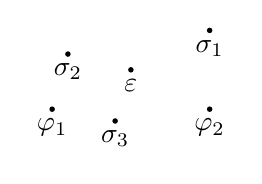
\begin{tikzpicture}
\fill[black] circle(1pt) node[anchor = north] {$\varepsilon$};
\fill[black] (1,0.5) circle(1pt) node[anchor = north] {$\sigma_1$};
\fill[black] (1,-0.5) circle(1pt) node[anchor = north] {$\varphi_2$};
\fill[black] (-0.2,-0.65) circle(1pt) node[anchor = north] {$\sigma_3$};
\fill[black] (-1,-0.5) circle(1pt) node[anchor = north] {$\varphi_1$};
\fill[black] (-0.8,0.2) circle(1pt) node[anchor = north] {$\sigma_2$};
\end{tikzpicture}
\end{figure}
Хотілось би їх організувати під певними властивостями. Розглянемо гомоморфізм 
\[f \colon S_3 \to \mathbb{Z}_2, \qquad f(\sigma) = \begin{cases} \overline{0}, & \sigma \text{ -- парна;} \\ \overline{1}, & \sigma \text{ -- непарна.} \end{cases} 
\]
Тепер ці елементи ми хоч якось згрупуємо:
\begin{figure}[H]
\centering
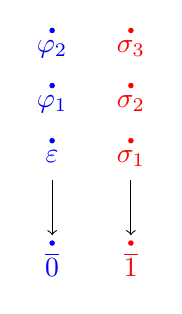
\begin{tikzpicture}
\fill[blue] (0,0) circle(1pt) node[anchor = north] {$\varepsilon$};
\fill[blue] (0,0.7) circle(1pt) node[anchor = north] {$\varphi_1$};
\fill[blue] (0,1.4) circle(1pt) node[anchor = north] {$\varphi_2$};
\fill[red] (1,0) circle(1pt) node[anchor = north] {$\sigma_1$};
\fill[red] (1,0.7) circle(1pt) node[anchor = north] {$\sigma_2$};
\fill[red] (1,1.4) circle(1pt) node[anchor = north] {$\sigma_3$};

\draw[->] (0,-0.5)--(0,-1.2);
\fill[blue] (0,-1.3) circle(1pt) node[anchor = north] {$\overline{0}$};
\draw[->] (1,-0.5)--(1,-1.2);
\fill[red] (1,-1.3) circle(1pt) node[anchor = north] {$\overline{1}$};
\end{tikzpicture}
\end{figure}
Тепер ми розглядаємо множину ${S_3}/_{\ker f}$ та зауважимо, що складається з двох множин, тобто
\[
{S_3}/_{\ker f} = \{\{\varepsilon, \varphi_1,\varphi_2\}, \{\sigma_1,\sigma_2,\sigma_3\}\} = \{A_3, S_3 \setminus A_3\} = {S_3}/_{A_3}.
\]
Якщо розглянути проєкцію $\pi \colon S_3 \to {S_3}/_{\ker f}$, то буде така картина:
\begin{figure}[H]
\centering
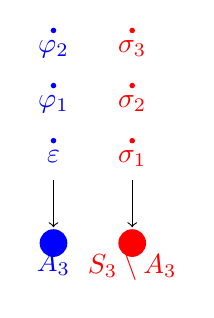
\begin{tikzpicture}
\fill[blue] (0,0) circle(1pt) node[anchor = north] {$\varepsilon$};
\fill[blue] (0,0.7) circle(1pt) node[anchor = north] {$\varphi_1$};
\fill[blue] (0,1.4) circle(1pt) node[anchor = north] {$\varphi_2$};
\fill[red] (1,0) circle(1pt) node[anchor = north] {$\sigma_1$};
\fill[red] (1,0.7) circle(1pt) node[anchor = north] {$\sigma_2$};
\fill[red] (1,1.4) circle(1pt) node[anchor = north] {$\sigma_3$};

\draw[->] (0,-0.5)--(0,-1.1);
\draw[->] (1,-0.5)--(1,-1.1);
\fill[blue] (0,-1.3) circle(5pt) node[anchor = north] {$A_3$};
\fill[red] (1,-1.3) circle(5pt) node[anchor = north] {$S_3 \setminus A_3$};
\end{tikzpicture}
\end{figure}
Тому очікується, що отримаємо ізоморфізм $\bar{f} \colon {S_3}/_{\ker f} \to \underset{=\mathbb{Z}_2}{\Im f}$, який описує останній малюнок:
\begin{figure}[H]
\centering
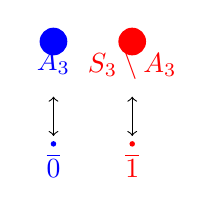
\begin{tikzpicture}
\fill[blue] (0,0) circle(5pt) node[anchor = north] {$A_3$};
\fill[red] (1,0) circle(5pt) node[anchor = north] {$S_3 \setminus A_3$};
\draw[<->] (0,-0.7)--(0,-1.2);
\fill[blue] (0,-1.3) circle(1pt) node[anchor = north] {$\overline{0}$};
\draw[<->] (1,-0.7)--(1,-1.2);
\fill[red] (1,-1.3) circle(1pt) node[anchor = north] {$\overline{1}$};
\end{tikzpicture}
\end{figure}
Резюмувати цей приклад можна ось таким крупним малюнком:
\begin{figure}[H]
\centering
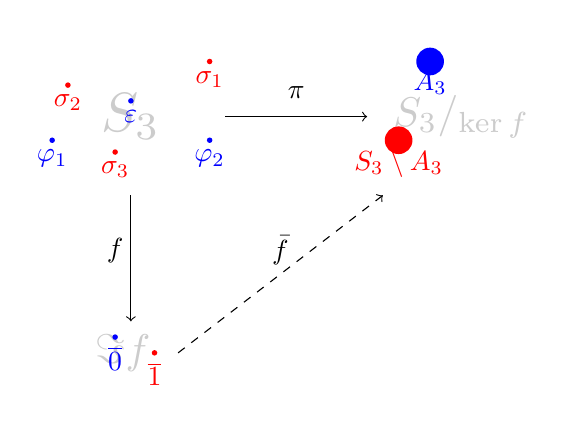
\begin{tikzpicture}
\node[black!20, circle, scale=2] at (0,-0.2) {$S_3$};
\fill[blue] circle(1pt) node[anchor = north] {$\varepsilon$};
\fill[red] (1,0.5) circle(1pt) node[anchor = north] {$\sigma_1$};
\fill[blue] (1,-0.5) circle(1pt) node[anchor = north] {$\varphi_2$};
\fill[red] (-0.2,-0.65) circle(1pt) node[anchor = north] {$\sigma_3$};
\fill[blue] (-1,-0.5) circle(1pt) node[anchor = north] {$\varphi_1$};
\fill[red] (-0.8,0.2) circle(1pt) node[anchor = north] {$\sigma_2$};
%Group G1

\draw[->] (1.2,-0.2)--(3,-0.2) node at (2.1,0.1) {$\pi$};

\node[black!20, circle, scale=1.5] at (4.2,-0.2) {$S_3/_{\ker f}$};
\fill[blue] (3.8,0.5) circle(5pt) node[anchor = north] {$A_3$};
\fill[red] (3.4,-0.5) circle(5pt) node[anchor = north] {$S_3 \setminus A_3$};
%Group G1/kerf

\draw[->] (0,-1.2) -- (0,-2.8) node at (-0.2,-1.9) {$f$};

\node[black!20, circle, scale=1.5] at (-0.1,-3.2) {$\Im f$};
\fill[blue] (-0.2,-3) circle(1pt) node[anchor = north] {$\overline{0}$};
\fill[red] (0.3,-3.2) circle(1pt) node[anchor = north] {$\overline{1}$};
%Group Imf

\draw [->, dashed] (0.6,-3.2) -- (3.2,-1.2) node at (1.9, -1.9) {$\bar{f}$};
\end{tikzpicture}
\end{figure}
Таким чином, ${S_3}/_{A_3} \cong \mathbb{Z}_2$.
\end{example}

\begin{example}
Маємо гомоморфізм $f \colon \mathbb{Z} \to \mathbb{Z}_n$ таким чином: $f(m) = \overline{m}$. Зрозуміло, що $\Im f = \mathbb{Z}_n$ та $\ker f = n \mathbb{Z}$. Отже, маємо $\mathbb{Z}/_{n \mathbb{Z}} \cong \mathbb{Z}_n$.\\
Насправді, якщо уважно подивитись, то $\mathbb{Z}/_{n \mathbb{Z}} = \mathbb{Z}_n$. Тож коли кажуть про адитивну групу класів лишків $\left< \mathbb{Z}/_{n \mathbb{Z}}, + \right>$, то здебільшого беруть таке позначення.
\end{example}

\begin{example}
Маємо гомоморфізм $f \colon D_n \to \mathbb{Z}_2$, що задається так: $r \overset{f}{\mapsto} \overline{0}$ та $s \overset{f}{\mapsto} \overline{1}$. Для інших елементів можна порахувати. Наприклад, $f(sr^2) = f(s) + f(r) + f(r)  = \overline{1} + \overline{0} + \overline{0} = \overline{1}$.\\
Можна зауважити, що $\Im f = \mathbb{Z}_2$ та $\ker f = \left<r\right>$. Отже, маємо $D_n/_{\left<r\right>} \cong \mathbb{Z}_2$.
\end{example}

\begin{example}
Маємо гомоморфізм $\det \colon \mathrm{GL}_n(\mathbb{R}) \to \mathbb{R} \setminus \{0\}$. Тут групи --- мультиплікативні. Можна показати, що $\Im \det = \mathbb{R} \setminus \{0\}$. Справді, $x \in \mathbb{R} \setminus \{0\}$:
\[ \det \begin{pmatrix}
x & 0 & \dots & 0 \\
0 & 1 & \dots & 0 \\
\vdots & \vdots & \ddots & \vdots \\
0 & 0 & \dots & 1 
\end{pmatrix} = x \text{ при } x \neq 0.
\]
Також неважко показати, що $\ker \det = \mathrm{SL}_n(\mathbb{R})$. Отже, ${\mathrm{GL}_n(\mathbb{R})}/_{\mathrm{SL}_n(\mathbb{R})} \cong \mathbb{R} \setminus \{0\}$.
\end{example}

\subsubsection{Друга теорема про ізоморфізм}
%Not necessarily
\iffalse
\begin{lemma}
Задано $\left< G, * \right>$ -- група, $H$ -- підгрупа $G$ та $N \triangleleft G$. Тоді $H \cap N \triangleleft H$.
\end{lemma}

\begin{proof}
Неважко переконатися, що $H \cap N$ буде підгрупою $H$.\\
Нехай $h \in H$ та $n \in H \cap N$. Хочемо довести, що $h * n * h^{-1} \in H \cap N$.\\
Оскільки $N \triangleleft G$ та при цьому $h \in G$, то $h*n*h^{-1} \in N$. Але водночас $h,n \in H \implies h*n*h^{-1} \in H$.\\
Разом отримаємо $h*n*h^{-1} \in H \cap N$.
\end{proof}
\fi

\begin{lemma}
Нехай $\left< G, * \right>$ --- група, $H \leq G$ та $N \triangleleft G$. Тоді $N \triangleleft H * N$.
\end{lemma}

\begin{proof}
Вимога $N \triangleleft G$ виправодується тим, що $H*N$ стає групою. А там вже неважко переконатися, що $N$ буде підгрупою $H*N$.\\
Нехай $u \in H*N$, тобто $u = h*n$, та $\tilde{n} \in N$. Хочемо довести, що $u*\tilde{n}*u^{-1} \in H*N$.\\
Маємо $u*\tilde{n}*u^{-1} = h*n*\tilde{n}*n^{-1}*h^{-1} = h*\bar{n}*h^{-1}$. Але оскільки $h \in G$ та $N \triangleleft G$, то $u*\tilde{n}*u^{-1} \in N$, тоді автоматично $u*\tilde{n}*u^{-1} \in H*N$.
\end{proof}

\begin{theorem}[Друга теорема про ізоморфізм]
Нехай $\left< G, * \right>$ --- група, $H \leq G$ та $N \triangleleft G$. Тоді
\begin{align*}
H/_{H \cap N} \cong (H*N)/_{N}.
\end{align*}
\end{theorem}

\begin{proof}
Установимо відображення 
\[
\varphi \colon H \to (H*N)/_N, \qquad h\mapsto h*N.
\] 
Ясно, що це гомоморфізм. Тоді за першою теоремою про ізоморфізм $H/_{\ker \varphi} \cong \Im \varphi$.\\
Доведемо, що $\ker \varphi = H \cap N$. Маємо $h \in \ker \varphi$, тоді $\varphi(h) = e*N \iff h*N = N \iff h \in N$. Але оскільки $\ker \varphi \triangleleft H$, то звідси $h \in H$, але водночс $h \in N$. Тож $h \in H \cap N$. Остаточно звідси $\ker \varphi = H \cap N$. До речі, $H \cap N = \ker \varphi \triangleleft H$.\\
Доведемо, що $\Im \varphi = (H*N)/_N$, а це теж саме, що показати, що $\varphi$ буде сюр'єктивним відображенням. Нехай $(h*n)N \in (H*N)/_N$. Треба зауважити, що $(h*n)*N = h*N$, просто тому що $h^{-1}*(h*n) = n \in N$. Тобто ми знайшли $h \in H$, для якого $\varphi(h) =h*N = (h*n)*N$.\\
Нарешті, $H/_{H \cap N} \cong (H*N)/_N$.
\end{proof}

%not necessarily
\iffalse
\begin{remark}
До речі, коли ми шукали ядро, ми одночасно довели, що $H \cap N = \ker \varphi \triangleleft H$, тобто перша лема могла бути зайвою. (*)
\end{remark}
\fi

\subsubsection{Третя теорема про ізоморфізм}
\begin{theorem}[Теорема про відповідність]
Нехай $\left< G, * \right>$ --- група та $N \triangleleft G$. Тоді існує бієкція $F \colon U_1 \to U_2$, де \[
U_1 = \{ H \text{ -- підгрупа } G \mid H \supset N\}, \qquad U_2 = \left\{ K \text{ -- підгрупа } G/_N\right\}.
\]
Тобто ця теорема каже, що є взаємна однозначність між підгрупами $G$, що містять $N$, а також підгрупами $G/_N$.
\end{theorem}

(\textit{хтось ще інколи це називає четвертою теоремою про ізоморфізм}.)

\begin{proof}
Установимо відображення 
\[ F \colon U_1 \to U_2, \qquad F(H) = \pi(H),\ \pi \colon G \to G/_N \text{ --- проєкція}.
\]
Можна зауважити, що 
\[
\pi(H) = \{g*N \mid g \in H\} = H/_N
\]
(\textit{оскільки $N = \ker \pi$, тоді автоматично $N \triangleleft H$}). Покажемо, що це бієктивне відображення.\\
Нехай $K$ --- підгрупа $G/_N$. Побудуємо множину $H = \{g \in G \mid g*N \in K\}$. Доведемо, що $H \in U_1$, тобто треба довести, що $H$ -- підгрупа $G$, а також $H \supset N$.\\
Для початку $H \neq \emptyset$, оскільки $e \in H$, просто тому що $e*N \in K$ в силу того, що $K$ --- підгрупа $G/_N$.\\
Нехай $x,y \in H$, тобто $x*N,y*N \in K$. Тоді звідси $(x*N)*(y*N)^{-1} \in K$, просто тому що $K$ --- підгрупа $G/_N$. Але з іншого боку $(x*N)*(y*N)^{-1} = (x*y^{-1})*N \in K$, а тому $x*y^{-1} \in H$.\\
Далі, $H \supset N$, тому що $K$ містить елемент $e*N = N$, а тому $H$ має всі елементи з $N$.\\
Нарешті, зауважимо, що $K = H/_N$, за побудовою підгрупи.\\
Отже, для кожної $K \in U_2$ знайшли $H \in U_1$, де $F(H) = \pi(H) = H/_N = K$ --- сюр'єктивність доведена.\\
Нехай $F(H_1) = F(H_2)$, тобто $H_1/_N = H_2/_N$. Доведемо, що $H_1 = H_2$.\\
Маємо $x \in H_1$, тоді $x*N \in H_1/_N = H_2/_N$, але тоді звідси $x \in H_2$. У зворотний бік абсолютно аналогічно --- ін'єктивність доведена.
\end{proof}

\begin{remark}
Зауважимо, що якщо $H \triangleleft G$, то тоді $K = H/_N \triangleleft G/_N$. Навпаки: якщо $H/_N \triangleleft G/_N$, то з урахуванням умови $N \triangleleft G$ та умови $N \subset H \subset G$, одержимо $H \triangleleft G$. Власне кажучи, можна тоді отримати таку бієкцію:
\begin{align*}
\{  H \triangleleft G \mid H \supset N \} \longleftrightarrow \{ H/_N \triangleleft G/_N \}.
\end{align*}
\end{remark}

\begin{lemma}
Нехай $\left< G, *\right>$ --- група, $M,N \triangleleft G$ та $N \leq M$. Тоді $N \triangleleft M$.
\end{lemma}

\begin{proof}
Дійсно, нехай $n \in N$ та $m \in M$. Тоді автоматично $m \in G$. Оскільки $N \triangleleft G$, то звідси $m*n*m^{-1} \in N$. Отже, $N \triangleleft M$.
\end{proof}

\begin{theorem}[Третя теорема про ізоморфізм]
Нехай $\left< G, *\right>$ -- група, $M,N \triangleleft G$ та $N \leq M$. Тоді
\begin{align*}
{G/_N}/_{M/_N} \cong G/_M.
\end{align*}
\end{theorem}

\begin{proof}
Передусім $M$ --- підгрупа $G$, що містить $N$, тож за відповідністю, $M/_N$ --- підгрупа $G/_N$, причому вона буде нормальною, оскільки $M \triangleleft G$. Тому далі все буде коректно визначено.\\
Розглянемо відображення 
\[
\varphi \colon G \to {G/_N}/_{M/_N}, \qquad \varphi = \pi_2 \circ \pi_1. 
\]
Тут дві проєкції $\pi_1 \colon G \to G/_N$ та $\pi_2 \colon G/_N \to {G/_N}/_{M/_N}$. Відображення $\varphi$ --- сюр'єктивний гомоморфізм, як композиція сюр'єктивних гомоморфізмів. Знайдемо ядро:
\[
\ker \varphi = \left\{g \in G \mid \varphi(g) = e*G/_M \right\} = \left\{ g \in G \mid (g*N)*M/_N = M/_N \right\} = \{g \in G \mid g*N \in M/_N\} = M.
\]
Щодо останньої рівності. Нехай $g \in G$ такий, що $g*N \in M/_N$. Тож $g*N = m*N$ при деякому $m \in M$, звідси $g = m*n$ при деякому $n \in N$. Але оскільки $N$ --- підгрупа $M$, то звідси $g \in M$.\\
Тепер нехай $g \in M$, звідси автоматично $g*N \in M/_N$.\\
За першою теоремою про ізоморфізм $G/_M \cong {G/_N}/_{M/_N}$.
\end{proof}


%Another proof without using correpsondence theorem
\iffalse
\begin{proof}
Установимо відображення $\varphi \colon G/_N \to G/_M$ таким чином: $g*N \mapsto g*M$.\\
Доведемо, що $\varphi$ є коректно визначеною функцією. Тому що дійсно, якщо є $g_1*N = g_2*N$, тоді $\varphi(g_1*N) = g_1*M$ та $\varphi(g_2*N) = g_2*M$ -- передали, по суті, один аргумент, а чи отримали одне й те саме, під питанням.\\
Оскільки $g_1*N = g_2*N$, то звідси $g_1*g_2^{-1} \in N$, але тоді $g_1*g_2^{-1} \in M$, тобто $g_1*M = g_2*M$. Отже, $\varphi(g_1*N) = \varphi(g_2*N)$.\\
$\varphi$ -- гомоморфізм, і це неважко:\\
$\varphi((g_1*N)*(g_2*N)) = \varphi((g_1*g_2)*N) = (g_1*g_2)*M = (g_1*M)*(g_2*M) = \varphi(g_1*N) * \varphi(g_2*N)$.\\
$\varphi$ -- сюр'єктивне відображення, бо якщо $g*M \in G/_M$, то тоді завжди можна знайти $g*N \in G/_N$, щоб $\varphi(g*N) = g*M$. Отже $\Im \varphi = G/_M$.\\
Нехай $g*N \in \ker \varphi$, або $\varphi(g*N) = e*M \iff g*M = M \iff \\ g \in M \iff g*N \in M/_N$, оскільки $g \in M$. Отже, $\ker \varphi = M/_N$.\\
За першою теоремою, про ізоморфізм, отримали ${G/_N}/_{M/_N} \cong G/_M$.
\end{proof}
\fi
\newpage

%end Теорія груп
%\fi

%start Теорія групової дії
%\iffalse
\section{Теорія групової дії}
\subsection{Дія групи}
\begin{definition}
Нехай $\left< G,*\right>$ --- група та $A$ --- деяка непорожня множина.\\
\textbf{Дією (ліворуч) групи $G$ на множину $A$} назвемо відображення $\rho \colon G \times A \to A$, з умовами нижче:
\begin{align*}
\forall a \in A: \rho(e_G,a) = a; \\
\forall g_1,g_2 \in G: \forall a \in A: \rho(g_1*g_2,a) = \rho(g_1,\rho(g_2,a)).
\end{align*}
Частіше замість $\rho(g,a)$ пишуть компактніше $ga$. Тоді умови переписуються так:
\begin{align*}
\forall a \in A: e_G a = a; \\
\forall g_1,g_2 \in G: \forall a \in A: (g_1 * g_2)a = g_1(g_2a).
\end{align*} 
\end{definition}

\begin{example}
Візьмемо дієдричну групу $D_4$ та множину $\mathbb{R}^2$. Ми встановимо дію таким чином:
\[
r \begin{pmatrix}
x \\ y
\end{pmatrix} = \begin{pmatrix}
0 & -1 \\
1 & 0
\end{pmatrix} \begin{pmatrix}
x \\ y
\end{pmatrix},
\]
де дана матриця описує матрицю повороту на $90^\circ$ проти годинникової стрілки відносно початку координат.
\[
s \begin{pmatrix}
x \\ y
\end{pmatrix} = \begin{pmatrix}
1 & 0 \\
0 & -1
\end{pmatrix} \begin{pmatrix}
x \\ y
\end{pmatrix},
\]
де дана матриця описує відбиття площини по $OY$.
\[
e \begin{pmatrix}
x \\ y
\end{pmatrix} = \begin{pmatrix}
1 & 0 \\
0 & 1
\end{pmatrix} \begin{pmatrix}
x \\ y
\end{pmatrix},
\]
де дана матриця нічого не змінює.\\
Решта дій буде композицією, яка описується множення матриць. Наприклад, 
\[
r^2 \begin{pmatrix}
x \\ y
\end{pmatrix} = \begin{pmatrix}
1 & 0 \\
0 & -1
\end{pmatrix} \begin{pmatrix}
1 & 0 \\
0 & -1
\end{pmatrix} \begin{pmatrix}
x \\ y
\end{pmatrix}.
\]
\end{example}

\begin{example}
Розглянемо знову дієдричну групу $D_4$ та простір $\Omega = \{ HH, HT, TH, TT \}$. Дана множина характеризуватиме ситуацію, коли на столі лежать дві монети поруч, що показують або орла (\textit{head}) або решку (\textit{tail}). Установимо дію групи $D_4$ на $\Omega$ таким чином:\\
$r \omega$ --- повернути ліву монету (наприклад, $r (HT) = TT$;\\
$s \omega$ --- змінити місцями монети (наприклад, $s(HT) = TH$.
\end{example}

\begin{example}
Нехай $\left< G,*\right>$ --- група. Розглянемо операцію $G$ як відображення $\rho \colon G \times G \to G$ як
\[ 
\rho(g_1,g_2) = g_1*g_2
\]
(\textit{множення в нашій групі}). Тоді це теж задає так звану \textbf{дію групи $G$ на собі (ліворуч)}. Дійсно,
\begin{align*}
\rho(e,g) = e*g = g; \\
\rho(g_1*g_2,h) = (g_1*g_2)*h = g_1*(g_2*h) = \rho(g_1,g_2*h) = \rho(g_1,\rho(g_2,h)).
\end{align*}
\end{example}

\begin{proposition}
Нехай $\left< G,*\right>$ --- група та $A$ --- деяка непорожня множина. Тоді кожна дія $\rho$ групи $G$ на множину $A$ індукує гомоморфізм $\sigma \colon G \to S_A$ формулою
\begin{align*}
\sigma (g)(a) = \rho(g,a), \forall a \in A.
\end{align*}
І навпаки: кожний гомоморфізм $\sigma \colon G \to S_A$ індукує дію групи $G$ на множину $A$ формулою вище.
\end{proposition}

\begin{proof}
\rightproof Дано: $\rho \colon G \times A \to A$ --- групова дія. Для кожного $g \in G$ формула $\sigma(g)(a) = \rho(g,a)$ буде визначати відображення $\sigma(g) \colon A \to A$.
\begin{enumerate}[wide=0pt,label={\Roman*.}]
\item \textit{$\sigma(g) \in S_A$, тобто $\sigma(g)$ задає бієкцію на $A$}.\\
Зауважимо, що для нейтрального елемента маємо
\[
\sigma(e_G)(a) = \rho(e_G,a) = a,\ \forall a \in A.
\]
Іншими словами, $\sigma(e_G) = \id_A$. Тепер, для $\sigma(g)$ стверджую, що $\sigma(g^{-1})$ буде оберненим відображенням. Справді,
\[
\sigma(g) \circ \sigma(g^{-1}) (a) = \sigma(g)(\rho(g^{-1},a)) = \rho(g, \rho(g^{-1},a)) = \rho(gg^{-1},a) = \rho(e_G,a) = a.
\]
Отже, $\sigma(g) \circ \sigma(g^{-1}) = \id_A$. Аналогічно доводиться, що $\sigma(g^{-1}) \circ \sigma(g) = \id_A$.

\item \textit{$\sigma$ задає гомоморфізм}.\\
Нехай $g_1, g_2 \in G$. Тоді
\[
\sigma (g_1*g_2)(a) = \rho(g_1*g_2,a) = \rho(g_1, \rho(g_2,a)) = \sigma(g_1)[\sigma(g_2)(a)] = (\sigma(g_1) \circ \sigma(g_2))(a).
\]
Коротше кажучи, $\sigma(g_1*g_2) = \sigma(g_1) \circ \sigma(g_2)$.
\end{enumerate}
\leftproof Дано: $\sigma \colon G \to S_A$ --- гомоморфізм. Доведемо, воно індукує дію. Позначимо $\rho(g,a) = \sigma(g)(a)$.\\
Оскільки $\sigma$ -- гомоморфізм, то звідси $\sigma(e_G) = \id_A$, зокрема це означає, що
\[
\sigma(e_G)(a) = \rho(e_G,a) = a.
\]
За аналогічною причиною $\sigma(g_1*g_2) = \sigma(g_1) \circ \sigma(g_2)$, зокрема це означає, що
\[
\rho(g_1*g_2,a) = \sigma(g_1)(\sigma(g_2)(a)) = \rho(g_1, \sigma(g_2)(a)) = \rho(g_1, \rho(g_2,a)). \qedhere
\]
\end{proof}

\begin{example}
\label{diredral_group_action}
Розглянемо дієдричну групу $D_3$, а також множину $A = \{1,2,3\}$.
\begin{enumerate}[wide=0pt]
\item Оберемо підгрупу $[r] \leq D_3$. Дію $\rho$ групи $[r]$ на множину $A$ задамо таким чином: $r$ діє на елемент $a \in A$ як поворот трикутника проти годинникової стрілки. Наприклад, $\rho(r^2,1) = 2,\ \rho(r^2,2) = 3,\ \rho(r^2,3) = 1$.\\
За щойно доведеним твердженням ця дія $\rho$ відповідає гомоморфізму $\sigma \colon [r] \to S_3$ таким чином:
\[
e \mapsto \begin{cases} 1 \mapsto 1; \\ 2 \mapsto 2; \\ 3 \mapsto 3; \end{cases},\ r \mapsto \begin{cases} 1 \mapsto 3; \\ 2 \mapsto 1; \\ 3 \mapsto 2; \end{cases},\ r^2 \mapsto \begin{cases} 1 \mapsto 2; \\ 2 \mapsto 3; \\ 3 \mapsto 1. \end{cases}
\]
Іншими словами $\sigma(e) = (1),\ \sigma(r) = (132),\ \sigma(r^2) = (123)$.

\item Оберемо підгрупу $[s] \leq D_3$. Дію $\rho$ групи $[s]$ на множину $A$ задамо таким чином: $r$ діє на елемент $a \in A$ як відбиття трикутника відносно осі, що проходить через цю вершину. Наприклад, $\rho(s,1) = 1,\ \rho(s,2) = 3,\ \rho(s,3) = 2$.\\
За твердженням це діє $\rho$ відповідає гомоморфізму $\sigma \colon [s] \to S_3$ таким чином:
\[
e \mapsto \begin{cases} 1 \mapsto 1; \\ 2 \mapsto 2; \\ 3 \mapsto 3; \end{cases},\ s \mapsto \begin{cases} 1 \mapsto 1; \\ 2 \mapsto 3; \\ 3 \mapsto 2. \end{cases}
\]
Іншими словами, $\sigma(e) = (1),\ \sigma(s) = (23)$.
\end{enumerate}
\end{example}

\subsection{Точні та вільні дії}
\begin{definition}
Дія групи $G$ на множині $A$ називається \textbf{точною}, якщо
\begin{align*}
(\forall a \in A: ga = a) \implies g = e.
\end{align*}
\end{definition}

\begin{proposition}
Дія групи $G$ на множині $A$ точна $\iff$ відображення $\sigma \colon G \to S_A$ --- ін'єктивне.\\
\textit{Вправа: довести.}
\end{proposition}

\begin{example}
Всі дії з того прикладу -- точні.
\end{example}

\begin{definition}
Дія групи $\left< G,*\right>$ на множині $A$ називається \textbf{вільною}, якщо
\begin{align*}
(\exists a \in A: ga = a) \implies g = e.
\end{align*}
\end{definition}

\begin{remark}
Будь-яка вільна дія --- точна дія.
\end{remark}

\begin{example}
Знову повертаємось до \exref{diredral_group_action}. Перша дія --- вільна, а друга дія --- ні.
\end{example}

\begin{example}
Дія групи $G$ на собі ліворуч --- вільна. Дійсно, якщо $g,h \in G$ такі, що $g*h = h$, то миттєво $g = e$. Це допоможе нам при доведенні наступної теореми.
\end{example}

\begin{theorem}[Теорема Келі]
Нехай $G$ --- група. Тоді існує підгрупа перестановок $H \leq S_G$, для якої $G \cong H$.\\
\textit{Уже така теорема була. Доведемо з іншого ракурсу цю теорему.}
\end{theorem}

\begin{proof}
Розглянемо дію групи $G$ на собі множенням зліва. Тоді вона задає гомоморфізм $\sigma \colon G \to S_G$. Але оскільки дія --- вільна (\textit{тому автоматично точна}), то $\ker \sigma = \{e\}$, тому що відображення ін'єктивне. Тоді $G \cong \Im \sigma$, причому $\Im \sigma$ --- шукана підгрупа $S_G$.
\end{proof}

\subsection{Орбіта елемента}
\begin{definition}
Нехай $G$ --- група, що діє на непорожню множину $A$.\\
\textbf{Орбітою елемента $a \in A$} називають таку підмножину:
\begin{align*}
\Orb_G(a) = \{ga \mid g \in G\}
\end{align*}
(\textit{тобто ми фіксуємо елемент $a \in A$ та розглядаємо всі можливі дії}).
\end{definition}

\begin{remark}
Зрозуміло, що $\Orb_G(a) \neq \emptyset$, просто тому що $a \in \Orb_G(a)$, бо $e_G a = a$.
\end{remark}

\begin{definition}
Орбіта називатиметься \textbf{тривіальною}, якщо
\begin{align*}
\Orb_G(a) = \{a\}.
\end{align*}
У такому разі для всіх $g \in G$ маємо $ga = a$. Таку точку $a$ називають \textbf{нерухомою}. 
\end{definition}

\begin{example}
Зокрема за \exref{diredral_group_action}, якщо взяти другу дію групи $[s]$ на множину $A$, отримаємо
\[
\Orb_{[s]}(1) = \{1\}, \qquad \Orb_{[s]}(2) = \Orb_{[s]}(3) = \{2,3\}.
\]
\end{example}

\begin{proposition}
Орбіти $\Orb_G(a)$ утворюють розбиття множини $A$.
\end{proposition}

\begin{proof}
Припустимо, що $\Orb_G(a) \cap \Orb_G(b) \neq \emptyset$ для деяких $a,b \in A$. Значить, мається там $c \in \Orb_G(a) \cap \Orb_G(b)$ таким чином, що $c = g_1 a = g_2 b$ для $g_1,g_2 \in G$. Звідси одержимо $a = g_1^{-1} g_2 b$. Ми зараз доведемо, що $\Orb_G(a) = \Orb_G(b)$.\\
Нехай $x \in \Orb_G(a)$, тобто $x = ga$ для деякого $g \in A$. Значить, тоді 
\[
x = g((g_1^{-1}*g_2) b) = [g*(g_1^{-1}*g_2)] b,
\]
причому тут $g*(g_1^{-1}*g_2) \in G$, а тому звідси $x \in \Orb_G(b)$.\\
Аналогічним чином із $x \in \Orb_G(a)$ випливає $x \in \Orb_G(b)$.
\end{proof}

\begin{definition}
Дія групи $G$ на множину $A$ називається \textbf{транзитивною}, якщо
\begin{align*}
\forall a,b \in A: \exists g \in G: b = ga.
\end{align*}
(\textit{тобто між будь-якими двома елементами можна законектитися, завдяки елементу, який діє}).
\end{definition}

\begin{remark}
Дія групи на множину транзитивна $\iff$ дана дія має єдину орбіту.
\end{remark}

\begin{example}
Узявши першу дію з \exref{diredral_group_action}, там $\Orb_{[r]}(1) = A$ --- і це єдина орбіта в принципі. Тобто дія $[r]$ на $A$ транзитивна.
\end{example}

\subsection{Стабілізатор}
\begin{definition}
Нехай $G$ --- група, яка діє на множину $A \neq \emptyset$.\\
\textbf{Стабілізатором елемента $a \in A$} називають множину\footnote{Частіше можна зустріти позначення стабілізатора $G_a$.}
\begin{align*}
\Stab_G(a) = \{g \in G \mid ga = a\}.
\end{align*}
(\textit{тобто тут всі елементи групи $g$, для яких точка $a \in A$ буде нерухомою}).
\end{definition}

\begin{proposition}
$\Stab_G(a)$ --- підгрупа $G$.
\end{proposition}

\begin{proof}
Цілком зрозуміло, що $\Stab_G(a) \neq \emptyset$, просто тому що $e \in \Stab_G(a)$.\\
Нехай $u,v \in \Stab_G(a)$, тобто $ua = a$ та $va = a$. Тоді
\begin{gather*}
(u*v)a = u(va) = ua = a \implies u*v \in \Stab_G(a); \\
a = ea = (u^{-1}*u)a = u^{-1}(ua) = u^{-1}a \implies u^{-1} \in \Stab_G(a). \qedhere
\end{gather*}
\end{proof}

\begin{lemma}
Існує бієкція $\alpha \colon G/_{\Stab_G(a)} \to \Orb_G(a)\footnote{Хоча $\Stab_G(a) \centernot\triangleleft G$ загалом, але множина $G/_{\Stab_G(a)}$ все одно визначається як просто клас всіх лівих суміжних класів.}$, де 
\[
\alpha(g*\Stab_G(a)) = ga.
\]
\end{lemma}

\begin{proof}
\begin{enumerate}[topsep=0pt,wide=0pt,label={\Roman*.}]
\item \textit{$\alpha$ коректно визначене}.\\
Нехай $g_1*\Stab_G(a) = g_2*\Stab_G(a)$, тобто звідси $g_1*g_2^{-1} \in \Stab_G(a)$, внаслідок чого $(g_1*g_2^{-1})a = a$. Тоді одержимо $g_1a = g_2a$.

\item \textit{$\alpha$ бієктивне}.\\
Нехай $\alpha(g_1*\Stab_G(a)) = \alpha(g_2*\Stab_G(a))$, тобто $g_1a = g_2a$, тоді звідси $(g_1*g_2^{-1})a = a$, тобто $g_1*g_2^{-1} \in \Stab_G(a)$ або $g_1*\Stab_G(a) = g_2*\Stab_G(a)$.\\
Нехай $x \in \Orb_G(a)$, тобто $x = ga$. Тоді існує $g*\Stab_G(a) \in G/_{\Stab_G(a)}$, де $\alpha(g*\Stab_G(a)) = ga = x$.\\
Довели, що $\alpha$ --- бієктивне відображення. \qedhere
\end{enumerate}
\end{proof}

Коротше кажучи, в нас комутує ось така діаграма:
\begin{figure}[H]
\centering
\begin{tikzcd}
G/_{\Stab_G(a)} \arrow[rr,"\alpha"] & & \Orb_G(a) \\
& G \arrow[lu,"g \mapsto g*\Stab_G(a)"] \arrow[ru,swap,"g \mapsto ga"]
\end{tikzcd}
\end{figure}

Із даної леми випливає миттєвво теорема:

\begin{theorem}
\label{cardinality_of_orbit_as_index_of_stabilizer}
Нехай $G$ --- скінченна група, яка діє на $A \neq \emptyset$. Тоді
\begin{align*}
\card(\Orb_G(a)) = [G:\Stab_G(a)].
\end{align*}
\end{theorem}

\begin{example}
Маємо циклічну групу $G$ порядка $35$, що діє на множину $A$, де $\card(A) = 4$. За щойно доведеною теоремою $\card(\Orb_G(a)) = [G : \Stab_G(a)]$, тобто $\card(\Orb_G(a)) \mid \card(G) = 35$, звідси маємо $\card(\Orb_G(a)) \in \{1,5,7,35\}$. Водночас $\Orb_G(a) \subset A$, тобто $\card(\Orb_G(a)) \leq 4$.\\
Разом отримаємо $\card(\Orb_G(a)) = 1$, тож дія групи $G$ на $A$ буде тривіальною, бо всі орбіти --- тривіальні. 
\end{example}

\begin{remark}
Означення нерухомої точки можна переписати інакше. Якщо $G$ --- група, яка діє на множину $A$, то точка $a \in A$ буде \textbf{нерухомою} $\iff \Stab_G(a) = G$.
\end{remark}

\subsection{Спряженість}
Одна особлива дія, яку часто розглядають в теорії груп. Вирішив її вставити окремим підрозділом, оскільки така дія варта своєї уваги.

\begin{definition}
Нехай $\left<G,*\right>$ --- група та $a \in G$.\\
Елемент $y \in G$ називається \textbf{спряженим до $a$}\footnote{Один із способів розглядати спряження як узагальнення зміни координат при переписуванні матриць або, з фізичної точки зору, як процес ''погляду на групу з іншої точки зору''. Дане зауваження було взято ось тут: \href{https://math.stackexchange.com/questions/11971/intuition-behind-conjugation-in-group-theory}{\textcolor{red}{*клік*}}.}, якщо
\begin{align*}
\exists x \in G: y = x*a*x^{-1}.
\end{align*}
Позначення: $y = a^x$.
\end{definition}

\begin{proposition}[Властивості спряженості]
Виконуються такі властивості:
\begin{enumerate}[nosep,wide=0pt,label={\arabic*)}]
\item $(a^x)^y = a^{y*x}$;
\item $(a*b)^x = a^x*b^x$;
\item $(a^x)^{-1} = (a^{-1})^x$.
\end{enumerate}
\end{proposition}

\begin{proof}
\begin{enumerate}[topsep=0pt,nosep,wide=0pt,label={\arabic*)}]
\item $(a^x)^y = y*a^x*y^{-1} = y*(x*a*x^{-1})*y^{-1} = (y*x) * a * (y*x)^{-1} = a^{x*y}$.
\item $(a*b)^x = x*(a*b)*x^{-1} = (x*a*x^{-1})*(x*b*x^{-1}) = a^x*b^x$.
\item $(a^x)^{-1} = (x*a*x^{-1})^{-1} = x*a^{-1}*x^{-1} = (a^{-1})^x$. \qedhere
\end{enumerate}
\end{proof}

\begin{proposition}
Відношення спряженості $a \sim y \iff y = a^x$ утворює відношення еквівалентності, тобто
\begin{enumerate}[topsep=0pt,nosep,wide=0pt,label={\arabic*)}]
\item $a^e = a$;
\item $b = a^x \iff a = b^{x^{-1}}$;
\item $b = a^x,\ c = b^y \implies c = a^{xy}$ (\textit{виконується через властивість 3)}).
\end{enumerate}
\end{proposition}

\begin{proposition}
Відображення $\rho \colon G \times G \to G$, що задається як $\rho(g,a) = a^g$, задає дію групи $\left<G,*\right>$ на собі.
\end{proposition}

\begin{proof}
Дійсно, маємо наступне:
\begin{gather*}
\rho(e,a) = a^e = a. \\
\rho(g_1*g_2,a) = a^{g_1*g_2} = (g_1*g_2)*a*(g_1*g_2)^{-1} = g_1*(g_2*a*g_2^{-1})*g_1^{-1} \\ = \rho(g_1,g_2*a*g_2^{-1}) = \rho(g_1,\rho(g_2,a)). \qedhere
\end{gather*}
\end{proof}

\textit{Позначення}: $a^G = \{ x*a*x^{-1} \mid x \in G\}$ --- клас спряжених елементів з $a$ (\textit{зауважимо, що, насправді кажучи, $a^G = \Orb_G(a)$}).

\begin{example}
Розглянемо кілька прикладів:
\begin{enumerate}[nosep,wide=0pt,label={\arabic*.}]
\item $e^G = \{e\}$ для кожної групи $\left<G,*\right>$.
\item $a^G$ містить один елемент $\iff G$ --- абелева група (\textit{вправа: довести}).
\item Розглянемо групу $\left< \mathrm{GL}_n(\mathbb{C}), \cdot \right>$. Тоді $B^{\mathrm{GL}_n(\mathbb{C})}$ --- клас спряжених елементів з $B$ --- це всі матриці $A$, що подібні з матрицею $B$. Для такихх матриць жорданова нормальна форма однакова.
\item Розглянемо групу $\left< Q_8, \cdot \right>$ --- кватерніони. Маємо класи спряженостей:
\begin{center}
$1^{Q_8} = \{1\},$ \hspace{0.5cm} $(-1)^{Q_8} = \{-1\},$ \hspace{0.5cm} $i^{Q_8} = \{-i,i\}$ (\textit{аналогічно $j,k$}).
\end{center}
\end{enumerate}
\end{example}

\begin{proposition}[Інший критерій нормальної підгрупи]
Нехай $G$ --- група та $H$ --- підгрупа. Тоді
\begin{align*}
H \triangleleft G \iff H = \displaystyle\bigcup_{h \in H} h^G.
\end{align*}
\end{proposition}

\begin{proof}
\rightproof Дано: $H \triangleleft G$, тобто $h^G = g*H*g^{-1} = H$, але тоді $\displaystyle\bigcup_{h \in H} h^G = H$.
\bigskip \\
\leftproof Дано: $\displaystyle\bigcup_{h \in H} h^G$, тоді $h^G = g*H*g^{-1} \subset H$ для всіх $g \in G$, тобто $H \triangleleft G$.
\end{proof}

\iffalse
\begin{corollary}
Задано $\left< G,*\right>$ -- скінченна група та $a \in G$. Тоді $\card(a^G) \mid \card(G)$.
\end{corollary}

\begin{proof}
Група $G$ діє сама на себе спряженням та $\Orb_G(a) = a^G$. Ми вже знаємо, що $\card(\Orb_G(a)) \mid \card(G)$, але це те, що ми хотіли.
\end{proof}
\fi

\subsection{Центр групи}
\begin{definition}
Нехай $\left< G, *\right>$ --- група.\\
\textbf{Центром} групи $G$ будемо називати таку множину:
\begin{align*}
Z(G) = \{ a \in G: \forall x \in G: a*x = x*a\}.
\end{align*}
Елементи $a \in Z(G)$ називають \textbf{центральними елементами} групи $G$.
\end{definition}

\begin{proposition}
Нехай $\left< G,*\right>$ --- група. Тоді $Z(G) \triangleleft G$, причому $Z(G)$ є абелевою (\textit{останнє є миттєвим}).
\end{proposition}

\begin{proof}
\begin{enumerate}[topsep=0pt,wide=0pt,label={\Roman*.}]
\item \textit{$Z(G)$ --- підгрупа $G$}.\\
Спершу зазначимо, що $Z(G) \neq \emptyset$, оскільки $e \in Z(G)$.\\
Нехай $a,b \in Z(G)$. Тоді хочемо довести, що $a*b^{-1} \in Z(G)$, і дійсно:
\[
a*b^{-1}*x = a*b^{-1}*x*b*b^{-1} \overset{b \in Z(G)}{=} a*b^{-1}*b*x*b^{-1} = a*x*b^{-1} \overset{a \in Z(G)}{=} x*a*b^{-1}.
\]

\item \textit{$Z(G)$ --- нормальна підгрупа $G$}.\\
Нехай $g \in G$ та $h \in G$. Хочемо довести, що $h*g*h^{-1} \in Z(G)$, справді:
\[
g*h*g^{-1}*x = g*g^{-1}*h*x = h*x = x*h = x*h*g*g^{-1} = x*g*h*g^{-1}. \qedhere
\]
\end{enumerate}
\end{proof}

\begin{proposition}
Нехай $\left<G,*\right>$ та $\left<H, \star \right>$ --- групи, а також $f \colon G \to H$ --- сюр'єктивний гомоморфізм. Тоді $f(Z(G)) \subset Z(H)$.
\end{proposition}

\begin{proof}
Нехай $u \in f(Z(G))$, тобто $u = f(g)$ при деякому $g \in Z(G)$. Доведемо, що $u \in Z(H)$.\\
Зафіксуємо $v \in H$. Оскільки $f$ --- сюр'єктивний, то звідси існує $a \in G$, для якого $v = f(a)$. Значить,
\[
v \star u = f(a) \star f(g) = f(a*g) \overset{g \in Z(G)}{=} f(g*a) = f(g) \star f(a) = u \star v.
\]
Отже, ми довели, що справді $u \in Z(H)$.
\end{proof}

\begin{proposition}
Група $\left< G,*\right>$ є абелевою $\iff Z(G) = G$.\\
\textit{Зрозуміло.}
\end{proposition}

\begin{lemma}
Дія спряженості є точною $\iff Z(G) = \{e\}$.
\end{lemma}

\begin{proof}
\rightproof Дано: спряжена дія --- точна. Нехай $x \in Z(G)$, тоді $x*g = g*x$, однак звідси $g = x*g*x^{-1}$, але з точності випливає, що $x = e$. Звідси одержимо $Z(G) = \{e\}$.
\bigskip \\
\leftproof Дано: $Z(G) = \{e\}$. Нехай $g*x*g^{-1} = x$ для всіх $g \in G$ та $x \in G$. Тоді звідси $g*x = x*g$, тобто $g \in Z(G) = \{e\}$, внаслідок чого $g = e$. Тому спряженість є точною дією.
\end{proof}

\begin{remark}
Точка $a \in G$ буде нерухомою (\textit{для дії спряженості}) $\iff a \in Z(G)$.\\
Отже, $Z(G)$ --- це множина всіх нерухомих точок для спряженості.
\end{remark}

\begin{example}
Зокрема маємо такі приклади:
\begin{enumerate}[nosep,wide=0pt]
\item $Z(S_3) = \{\varepsilon\}$ (\textit{значить, спряженість в групі $S_3$ буде точною});
\item $Z(Q_8) = \{1,-1\}$ (\textit{значить, спряженість в $Q_8$ буде неточною, а тому й невільною}).
\end{enumerate}
\end{example}

\subsection{Централізатори та $p$-групи}
\begin{definition}
Нехай $\left< G, *\right>$ --- група та $a \in G$.\\
\textbf{Централізатором\footnote{Інколи ще позначають централізатор за $C_G(a)$.} елемента $a$} називають таку множину\footnote{Взагалі-то кажучи, централізатор можна визначати від будь-якої підмножини $S \subset G$ таким чином: 
\[
Z_G(S) = \{g \in G: s*g = g*s,\ \forall s \in S\}.
\]
Те, що було записано в означенні, це лише частинний випадок при $S = \{a\}$ (\textit{тобто деякій одноточковій множині}).}:
\begin{align*}
Z_G(a) = \{g \in G: a*g = g*a\}.
\end{align*}
\end{definition}

\begin{remark}
$Z(G) = \displaystyle\bigcap_{a \in G} Z_G(a)$. \textit{(вправа: довести)}
\end{remark}

\begin{remark}
Розглянемо дію спряження. Тоді оскільки $a*g = g*a \iff g*a*g^{-1} = a$, то одержимо, що 
\[
\Stab_G(a) = Z_G(a).
\]
Внаслідок чого кількість елементів обріти обчислюється ось так:
\[
\card (a^G) = [G : Z_G(a)].
\]
Крім того, $Z(G)$ буде множиною всіх нерухомих точок в цій дії (вправа: \textit{усвідомити}).
\end{remark}

\begin{theorem}
Нехай $G$ --- група (\textit{розглянемо дію спряженості}) та $\Gamma_0 \subset G$ --- підмножина, яка містить рівно по одному представнику від кожного класа спряжності елемента $G$. Тоді
\begin{align*}
\card(G) = \displaystyle\sum_{a \in \Gamma_0} [G: Z_G(a)].
\end{align*}
Якщо позначити $\Gamma = \Gamma_0 \setminus Z(G)$, то можна переписати формулу:
\begin{align*}
\card(G) = \card(Z(G)) + \sum_{a \in \Gamma} [G: Z_G(a)].
\end{align*}
\end{theorem}

\begin{proof}
Із зауваження $Z(G)$ --- множина всіх нерухомих точок. Відомо, що $G$ розбивається орбітами, тобто 
\[
G = \displaystyle\bigsqcup_{a \in \Gamma_0} \Orb_G(a).
\]
Відповідно можна записати таку рівність:
\[
\card(G) = \displaystyle\sum_{a \in \Gamma_0} \card(\Orb_G(a)) = \sum_{a \in Z(G)} \card(\Orb_G(a)) + \sum_{a \in \Gamma} \card(\Orb_G(a)).
\]
Але ми знаємо, що $\card(\Orb_G(a)) = [G:Z_G(a)]$ із того самого зауваження. Також коли $a \in Z(G)$, то $\card(\Orb_G(a)) = 1$.
\end{proof}

\subsection{Нормалізатори}
Нехай $\left<G,*\right>$ --- група. Розгленмо дію групи $G$ на множину $2^G$ (\textit{клас всіх підмножин $G$}) ось так:
\begin{align*}
\rho(g,S) = g*S*g^{-1} \eqbydef \{g*s*g^{-1} \mid s \in S\}
\end{align*}
(\textit{щось схоже по типу на спряження, просто тепер з множинами}).

\begin{definition}
Нехай $\left< G, *\right>$ --- група та $S \subset G$ (\textit{не обов'язково підгрупа}).\\
\textbf{Нормалізатором\footnote{Якщо $ S \subset G$, то можна зауважити, що $Z_G(S) \subset N_G(S)$. Іншими словами, нормалізатор є послабленою версією централізатора.} підмножини $S$} називають таку множину:
\begin{align*}
N_G(S) = \{g \in G: g*S*g^{-1} = S\}.
\end{align*}
\end{definition}

\begin{remark}
Зважаючи, яку ми дію задали, тут насправді $N_G(S) = \Stab_G(S)$.
\end{remark}

% Inaccurate remark
\iffalse
\begin{remark}
Нормалізатор --- це в деякому сенсі узагальнення централізатора. Якщо в централізаторі ми фіксували $a \in G$, тобто одноточкову множину $\{a\}$, то в нормалізаторі ми фіксуємо аж підгрупу $H$ групи $G$.
\end{remark}
\fi

\begin{proposition}
Нехай $H$ є підгрупою $G$. Тоді $N_G(H)$ --- найбільша підгрупа $G$, що містить $H$, при цьому $H \triangleleft N_G(H)$.
\end{proposition}

\begin{proof}
\begin{enumerate}[topsep=0pt,wide=0pt,label={\Roman*.}]
\item \textit{$N_G(H)$ --- підгрупа $G$}. \\
Це дійсно так, просто тому що $\Stab_G(H)$ є підгрупою $G$.

\item \textit{$H \subset N_G(H)$}.\\
Нехай $a \in H$, тоді автоматично $a^{-1} \in H$. Але тоді
\[
a*H*a^{-1} = a*(H*a^{-1}) \overset{a^{-1} \in H}{=} a*H \overset{a \in H}{=} H.
\]
Таким чином, одержали $a \in N_G(H)$.

\item \textit{$H \triangleleft N_G(H)$} (\textit{вправа: довести}).

\item \textit{$N_H(G)$ --- найбільша така підгрупа}.\\
Припустимо тепер, що існує $M \supset N_G(H)$ --- більша підгрупа $G$, що містить $H$ та $H \triangleleft M$. Але тоді за нормальністю $\forall m \in M: H = m*H*m^{-1}$, тобто автоматично $m \in N_G(H)$, а тому $M \subset N_G(H)$. Отже, $M = N_G(H)$. \qedhere
\end{enumerate}
\end{proof}

\subsection{$p$-групи та деякі результати}
\begin{definition}
Нехай $p$ --- просте число. Скінченна група $G$ називається \textbf{$p$-групою}\footnote{
Можна ще прочитати таке, що група $G$ називається $p$-групою, якщо
\begin{align*}
\forall g \in G \setminus \{e\}: \ord (g) = p^{n} \text{ для деякого $n \geq 1$}.
\end{align*}
Для скінченних груп ці означення еквівалентні (\textit{див.\ інші вставки}). І в силу еквівалентності дане означення вирішили узагальнити для нескінченних груп. Прикладами є зокрема: групи Прюфера, так званий ''монстр Тарського'', а також (\textit{якщо щось про теорію полів знаєте}) нескінченно вимірний векторний простір над полем, що містить лише $p$ елементів (\textit{ну наприклад, $C[a,b]$ над $\mathbb{F}_p$}).
}, якщо
\begin{center}
$|G| = p^k$ для деякого $k \geq 0$. 
\end{center}
\end{definition}

\begin{theorem}
\label{amount_of_fixed_points}
Нехай $G$ --- скінченна $p$-група, яка діє на множину $A$. Позначимо $F$ за множину всіх нерухомих точок цієї дії. Тоді
\begin{align*}
\card(F) \equiv \card(A) \pmod {p}.
\end{align*}
\end{theorem}

\begin{proof}
За теоремою Лагранжа та \thref{cardinality_of_orbit_as_index_of_stabilizer} відомо вже, що
\[
|G| = |\Stab_G(a)| \cdot [G:\Stab_G(a)] = |\Stab_G(a)| \cdot \card(\Orb_G(a)).
\]
Маючи той факт, що $G$ є $p$-групою, тобто маючи $|G| = p^r$, отримаємо 
\[
\card(\Orb_G(a)) \mid p^r.
\]
Оскільки $p$ --- просте число, то звідси 
\[
\card(\Orb_G(a)) \in \{1,p,p^2,\dots,p^r\}.
\]
Якщо $a \in F$, то відомо, що $\card(\Orb_G(a)) = 1$ (\textit{оскільки $a$ --- нерухома точка}). Із цього випливає, що $p \mid \card(\Orb_G(a))$ для кожної точки $a \in A \setminus F$.\\
Доведемо, що орбіти точок із $A \setminus F$ утворюють розбиття $F$, тобто
\[
A \setminus F = \bigsqcup_{a \in A \setminus F} \Orb_G(a).
\]
Якщо $x \in A \setminus F$, то по-перше, $x \in \Orb_G(a)$ (\textit{оскільки орбіти утворюють розбиття множини $A$}), а по-друге, $a \in A \setminus F$ (\textit{у протилежному випадку $x$ сама стане нерухомою точкою, чого ми не вимагали}).\\
Якщо $x \in \Orb_G(a)$ при $a \in A \setminus F$, то тоді $x \in A \setminus F$ (\textit{якби $x$ була нерухомою, то, маючи $x = ga$ та $x = gx$, отримали би $x = a$, а це означало б нерухомість точки $a$, чого ми не вимагали}).\\
У результаті одержимо, що $p \mid \card(A \setminus F)$, але тоді
\[
\card A = \card (A \setminus F) + \card F \equiv \card F \pmod p. \qedhere
\]
\end{proof}

\begin{corollary}
Нехай $G$ --- нетривіальна скінченна $p$-група. Тоді $Z(G)$ --- нетривіальний.
\end{corollary}

\begin{proof}
Оскільки $Z(G)$ --- множина нерухомих точок (\textit{при спряженої дії}), то звідси 
\[
|G| \equiv |Z(G)| \pmod p.
\]
Однак оскільки $G$ є скінченною $p$-групою, то $p \mid |Z(G)|$, тому $Z(G)$ точно нетривіальний.
\end{proof}

%How to prove based on the formula above
\iffalse
\begin{proof}
Відомо, що $\card(G) = [G \!: \! Z_G(a)] \card(Z_G(a))$. Оскільки $\card(G) = p^r,\ r > 1$, то тоді отримаємо $p \mid [G \!: \! Z_G(a)]$ для всіх $a \in \Gamma$, тому що в цьому випадку $[G:Z_G(a)] = \card(\Orb_G(a)) > 1$ (ми беремо ті точки, де орбіта містить більше одного елементу). Тоді\\
$\card(Z(g)) = \card(G) - \displaystyle\sum_{a \in \Gamma}[G: Z_G(a)] \implies p \mid \card(Z(g))$.
\end{proof}
\fi

\begin{corollary}
Нехай $G$ --- група порядку $p^2$. Тоді $G$ --- абелева.
\end{corollary}

\begin{proof}
Уже $p$-група $G$ тут нетривіальна, а тому $Z(G)$ також буде нетривіальним. Оскільки $Z(G)$ є підгрупою $G$, то $\card(Z(G)) \in \{p,p^2\}$.\\
!Припустимо, що $\card(Z(G)) = p$, тобто існує елемент $a \in G \setminus Z(G)$. Оскільки $\{a\} \cup Z(G) \subset Z_G(a)$, то звідси $\card(Z_G(a)) > p$. Оскільки відомо, що $\card(Z_G(a)) \mid \card(G) = p^2$, то тоді обов'язково $\card(Z_G(a)) = p^2$, тобто звідси $Z_G(a) = G$. Отримали $a \in Z(G)$ --- суперечність!\\
Отже, обов'язково $\card(Z(G)) = p^2$, але тоді $Z(G) = G$.
\end{proof}

\begin{remark}
Якщо $|G| = p^k$ при $k > 2$, то ми не можемо сказати загалом, що $G$ є абелевою.
\end{remark}

\begin{example}
Зокрема дієдрична група $D_4$ містить $8 = 2^3$ елементів, але дана групу не є абелевою (\textit{ну дійсно, $sr \cdot r \neq r \cdot sr$}) (\textit{так само з $D_{2^{k-1}}$}).
\end{example}

(TODO: вставити приклад з групою Гайзенберга)

% TODO move somewhere else
\iffalse
\begin{definition}
Задано $\left< G, *\right>$ -- група, де $G \neq \{e\}$.\\
Група називається \textbf{простою}, якщо
\begin{align*}
\text{у групи $G$ немає власних нормальних підгруп, відмінних від $\{e\}$}
\end{align*}
\end{definition}

\begin{remark}
Тобто $\{e\}$ уже не буде простою групою.
\end{remark}
\fi

\subsection{Теорема Коші та Теореми Сілова}
\begin{theorem}[Теорема Коші]
Нехай $G$ --- скінченна група та $p$ --- просте число, причому $p \mid |G|$. Тоді існує елемент $g \in G$, для якого $\ord(g) = p$.
\end{theorem}

\textit{Увага! Спочатку доведення теореми проведемо для абелевих груп. Згодом потрібно буде дещо інше вивести, щоб довести теорему Коші в загальній формі.}

\begin{proof}
Доведення за МІ по таких порядках $|G|$, де $p \mid |G|$.
\begin{enumerate}[wide=0pt,nosep,label={\Roman*.}]
\item \textit{База індукції}. При $|G| = p$, за наслідком з теореми Лагранжа, група $G$ є циклічною. Тому такий елемент $g \in G$, що $\ord(g) = p$, точно існує.

\item \textit{Припущення індукції}. Теорема Коші виконується для груп, для яких просте число $p$ ділить їхній порядок, причому їхній порядок строго менший за $|G|$.

\item \textit{Крок індукції}. Доведемо теорему Коші для групи $G$ з порядком $|G|$. Нехай $x \in G \setminus \{e\}$, для зручності позначимо $\ord x = m$. Виникають два можливих випадки:
\begin{enumerate}[wide=0pt,label={\roman*)}]
\item $p \mid m$.\\
Тоді за \prpref{ord_g_to_some_power} відомо, що $\ord \left(x^{\frac{m}{p}} \right) = p$ --- закінчили.

\item $p \nmid m$.\\
Розглянемо тоді підгрупу $H = \left<x\right>$. Оскільки $G$ --- абелева, то $H \triangleleft G$, тобто можемо розглянути групу $G/_H$. Спочатку зазначимо, що $|G/_H| < |G|$, оскільки $|H| = \ord x = m > 1$. Крім того, $p \mid |G/_H|$, адже маємо $|G/_H| \cdot |H| = |G|$, де $p \mid |G|$, але $p \nmid |H|$.\\
Отже, за припущенням МІ існує елемент $y*H \in G/_H$, для якого $\ord(y*H) = p$. Але неважко переконатися, що $p = \ord(g*H) \mid \ord(y) = k$. Тоді знову $\ord\left(y^{\frac{k}{p}}\right) = p$ за \prpref{ord_g_to_some_power}.
\end{enumerate}
\end{enumerate}
МІ доведено.
\end{proof}

\begin{definition}
Нехай $G$ --- скінченна група та $p$ --- просте число. Із порядка $|G|$ відокремимо найбільший можливий степінь простого числа $p$, тобто буде
\[
|G| = p^r \cdot m, \qquad p \nmid m.
\]
\textbf{$p$-підгрупою Сілова} називають підгрупу порядка $p^r$ (\textit{коротше, найбільша скінченна $p$-підгрупа}).
\end{definition}

\iffalse
\noindent
Важливі питання, на які ми хочемо відповісти:
\begin{enumerate}[nosep,wide=0pt,label={\arabic*.}]
\item Чи існує завжди підгрупа Сілова?
\item Якщо їх кілька, як вони між собою пов'язані?
\item Що відомо за кількість підгруп Сілова?
\end{enumerate}
\fi

\begin{theorem}[І теорема Сілова (про існування)]
Нехай $G$ --- скінченна група та $p$ --- просте число. Тоді існує $p$-підгрупа Сілова.
\end{theorem}

Ми доведемо більш загальну теорему, після якої автоматично одержимо І теорему Сілова.

\begin{theorem}
Нехай $G$ --- скінченна група та $p$ --- просте число таке, що $p^k \mid \, |G|$. Тоді група $G$ містить підгрупу порядка $p^k$.
\end{theorem}

\begin{proof}
Доведення буде за МІ по $|G|$ (\textit{одразу кажу, що при $k = 0$ нічого цікавого}).
\begin{enumerate}[nosep,wide=0pt,label={\Roman*.}]
\item \textit{База індукції}. При $|G| = p$ --- нецікаво.

\item \textit{Припущення індукції}. Теорема спрацювує для будь-якої підгрупи $H$ так, що $|H| < |G|$.

\item \textit{Крок індукції}. Доведемо теорему саме для групи $G$. Для початку пригадаємо, що
\[
|G| = |Z(G)| + \sum_{a \in \Gamma} [G:Z_G(a)].
\]
Можуть виникнути два випадки:
\begin{enumerate}[nosep,wide=0pt,label={\roman*)}]
\item $p \nmid [G:Z_G(a)]$ (\textit{деякий індекс}).\\
Оскільки $p^k \mid |G|$, то обов'язково $p^k \mid |Z_G(a)|$ із теореми Лагранжа. Оскільки $|Z_G(a)| < |G|$, то за припущенням індукції $Z_G(a)$ містить підгрупу порядка $p^k$, тому зокрема й $G$ містить.

\item $p \mid [G:Z_G(a)]$ (\textit{всі індекси}).\\
Тоді одержимо, що $p \mid |Z(G)|$. За теоремою Коші для абелевих груп знайдеться елемент $g \in Z(G)$, для якого $\ord(g) = p$. Але тоді $[g] \triangleleft G$ в силу того, що $[g] \subset Z(G)$.\\
Тому розглянемо групу $G' = G/_{[g]}$. За теоремою Лагранжа $|G'| = \dfrac{|G|}{p}$. Оскільки $p^k \mid \, |G|$, тоді $p^{k-1} \mid \, |G'|$. Оскільки також $|G'| < |G|$, то за припущенням індукції $G'$ містить підгрупу $H'$ порядка $p^{k-1}$. Але нам відома відповідність:
\[
H' \leq G/_{[g]} \leftrightarrow \left<g\right> \subset H \leq G,
\]
тоді $H' = H/_{[g]}$. Нарешті, $|H| = p |H'| = p^k$, звідси $G$ містить підгрупу $H$ порядка $p^k$.
\end{enumerate}
\end{enumerate}
МІ доведено.
\iffalse
!Припустимо, що існує скінченна група $G$, просте число $p$, для яких хоч й існує $k \in \mathbb{N}$, для якого $p^k \mid \, |G|$, але при цьому $G$ не містить підгрупу порядка $p^k$ (\textit{ми оберемо групу $G$ з найменшим можливим порядком $|G|$, щоб виконувалося те, що ми припустили}). Тоді для всіх інших груп з меншим порядком, ніж $|G|$, I теорема Сілова виконуватиметься.\\
Хочемо довести, що $p \mid \, |Z(G)|$, де нам вже відомо, що $|G| = |Z(G)| + \displaystyle\sum_{a \in \Gamma} [G:Z_G(a)]$. Для цього залишилося довести, що $p$ ділить будь-який індекс підгрупи $G$.\\
!!Припустимо, що існує нетривіальна підгрупа $H$, для якої $p \nmid [G:H]$. Оскільки відомо, що $p^k \mid \, |G|$, то тоді обов'язково $p^k \mid \, |H|$ із теореми Лагранжа. Оскільки $|H| < |G|$, то тоді працює І теорема Сілова: $H$ містить підгрупу порядка $p^k$. Зрозуміло, що $G$ також --- суперечність!!\\
Із цього випливає зокрема, що $p \mid [G:Z_G(a)]$ для всіх $a \in \Gamma$.\\
Отже, маємо $p \mid |Z(G)|$. За теоремою Коші абелевих груп, знайдеться елемент $g \in Z(G)$, для якого $\ord(g) = p$. Але тоді $[g] \triangleleft G$ в силу того, що $[g] \subset Z(G)$.\\
Тому розглянемо групу $G' = G/_{[g]}$. За теоремою Лагранжа, $|G'| = \dfrac{|G|}{p}$. Оскільки $p^k \mid \, |G|$, тоді $p^{k-1} \mid \, |G'|$. Оскільки також $|G'| < |G|$, то працює І теорема Сілова: $G'$ містить підгрупу $H'$ порядка $p^{k-1}$. Але за відповідністю, $H'$ відповідає $H \supset [g]$ -- підгрупа $G$, зокрема тоді $H' = H/_{[g]}$.\\
Нарешті, $|H| = p |H'| = p^k$, звідси $G$ містить підгрупу $H$ порядка $p^k$ --- суперечність!
\fi
\end{proof}

\textit{До речі кажучи, повернемось тепер до теореми Коші}\footnote{Для доведення І теореми Сілова потрібна була теорема Коші для абелевих груп. Для узагальнення теореми Коші потрібна була І теорема Сілова. Саме тому я вирішив теореми з двома прізвищами поєднати в один підрозділ.}\textit{. Час довести це для неабелевих груп\footnote{Для допитливих залишу доведення, що два означення $p$-груп еквівалентні.\\
\rightproof Дано: $|G| = p^k$ для деякого $k \geq 1$ (якщо $G$ --- тривіальна, то нецікаво). Тоді для будь-якого $g \in G \setminus \{e\}$ маємо, що $\ord (g) \mid p^k$, тобто $\ord(g) = p^r$.
\bigskip \\
\leftproof Дано: для будь-якого $g \in G \setminus \{e\}$ маємо, що $\ord (g) = p^r$ для деякого $r \geq 1$. Найбільший можливий степінь числа $p$ позначу за $k$, тоді $p^k \mid |G|$. Тепер припустимо, що $q \mid |G|$, де $q \neq p$ --- будь-яке інше просте число, тоді існує підгрупа $H$, причому $|H| = q$. Обравши максимальний степінь числа $p$, скажімо $l$, одержимо, що $p^l \mid |H| = q$, але тоді $p \mid q$, що неможливо. Таким чином, $|G| = p^k$.
}.
}

\begin{proof}
Пригадаємо, що $p \mid |G|$. Тоді за щойно доведеною лемою існує підгрупа $H$, для якої $|H| = p$. За наслідком теореми Лагранжа така підгрупа --- циклічна. Значить $H = \left<h\right>$, причому $h \in G$, а також $\ord(h) = p$.
\end{proof}

\begin{theorem}[II теорема Сілова (про ''єдиність'')]
Нехай $G$ --- скінченна група та $p$ --- просте число. Нехай $P_1,P_2$ --- дві $p$-підгрупи Сілова (\textit{які існують за І теоремою}). Тоді $P_1,P_2$ --- спряжені (\textit{іншими словами, існує $g \in G$, для якого $P_2 = g*P_1*g^{-1}$}).
\end{theorem}

Знову доведемо більш загальну теорему, яка доведе ІІ теорему Сілова.

\begin{theorem}
Нехай $G$ --- скінченна група та $p$ --- просте число. Оберемо $p$-підгрупу Сілова $P$. Нехай $H$ --- $p$-підгрупа $G$. Тоді існує елемент $g \in G$, для якого $H \subset g*P*g^{-1}$.
\end{theorem}

\begin{proof}
Розглянемо дію групи $H$ множенням зліва на множини суміжних класів $G/_P$. У нас буде $h (a*P) = (h*a)*P$. Оскільки $|G/_P| = [G:P]$, тобто це буде взаємно просте число з $p$, то звідси дана дія містить нерухомі точки, за \crlref{amount_of_fixed_points}. Оберемо $a*P \in G/_P$ -- нерухома точка, тобто $h*a*P = a*P$, для всіх $h \in H$.\\
$\forall h \in H: h*a*P = a*P \implies \forall h \in H: a^{-1}*h*a*P = P \implies \forall h \in H: a^{-1}*h*a \in P \implies a^{-1}*H*a \subset P \implies H \subset a*P*a^{-1}$.
\end{proof}

\begin{theorem}[III теорема Сілова]
Нехай $G$ --- скінченна група та $p$ --- просте число. Маємо $|G| = p^r m,\ p \nmid m$. Позначимо $N_p$ за кількість $p$-підгруп Сілова групи $G$. Тоді
\begin{align*}
\begin{cases}
N_p \mid m; \\
N_p \equiv 1 \pmod p.
\end{cases}
\end{align*}
\end{theorem}

Для доведення даної теореми над знадобиться корисна лема.
\begin{lemma}
Нехай $\left< G, *\right>$ --- скінченна група та $P$ --- $p$-підгрупа Сілова. Нехай $P$ діє на $G/_P$ множенням лівих суміжних класів. Тоді
\begin{center}
$a*P \in G/_P$ --- нерухома точка $\iff a \in N_G(P)$.
\end{center}
Внаслідок чого кількість нерухомих точок даної дії дорівнює $[N_G(P):P]$.
\end{lemma}

\begin{proof}
Аналогічно, як це було з лемою при ІІ теорери Сілова, маємо, що $a*H$ --- нерухома точка $\iff P \subset a*P*a^{-1} \iff P = a*P*a^{-1}$ (\textit{у цих двож множинах однакова кількість елементів}). Останнє еквівалентне тому, що $a \in N_G(P)$.\\
Отже, всі нерухомі точки $a*P \in G/_P$ насправді потрапляють в ${N_G(P)}/_P$, кількість елементів яких якраз $[N_G(P):P]$, а це й буде кількість нерухомих точок.
\end{proof}

\iffalse
\begin{proof}
Аналогічно, як це було з ІІ теоремою Сілова, доведемо, що $a*H$ -- нерухома точка $\iff H \subset a*H*a^{-1}$.\\
Останнє еквівалентне тому, що $a \in N_G(H)$ (див. означення нормальних підгруп). А це теж саме, що $a*H \subset N_G(H)$.\\
Нарешті, оскільки $H \triangleleft N_G(H)$, то звідси $[N_G(H):H]$ -- кількість нерухомих точок.
\end{proof}
\fi

Маючи лему, тепер доведемо ІІІ теорему Сілова.

\begin{proof}
За І теоремою Сілова бодай одна $p$-підгрупи Сілова $P$ існує. За ІІ теоремою Сілова множина всіх $p$-підгруп Сілова --- це множина всіх спряжених до $P$. Якщо розглядати дію групи $G$ спряженням на $2^G$, то отримаємо, що $\Orb_G(P)$ --- це та сама множина, яка описує множину всіх спряжених до $P$, а до того ж $\Stab_G(P) = N_G(P)$. За умовою $N_p = |\Orb_G(P)|$, тоді ми знаємо, що
\[ 
N_p = [G: N_G(P)].
\]
Спочатку доведемо, що $N_p \mid m$. Дійсно,
\[
m = [G:P] = [G:N_G(P)] \cdot [N_G(P) : P] = N_p \cdot [N_G(P) : P].
\]
Залишилося довести, що $N_p \equiv 1 \pmod p$. Нехай $P$ діє на $G/_P$ множенням лівих суміжних класів. Позначимо $F$ за множину нерухомих точок. Тоді за щойно доведеною лемою $|F| = [N_G(P) : P]$. Оскільки $P$ є $p$-підгрупою, то з іншого твердження випливає, що 
\[
|F| \equiv |G/_P| \pmod p.
\]
Проте звідси одержимо, що
\[
[N_G(P) : P] \equiv m \pmod p.
\]
Знаючи, що $m = N_p \cdot [N_G(P):P]$, а також щойно одержану конгруенцію, отримаємо
\[
m \equiv m N_p \pmod p.
\]
Утім оскільки $p \nmid m$, то автоматом $N_p \equiv 1 \pmod p$.
\end{proof}

\subsection{Деякі результати, пов'язані з групами Сілова}
\begin{proposition}
Скінченна група $G$ має лише одну підгрупу Сілова $P \iff P \triangleleft G$.
\end{proposition}

\begin{proof}
\rightproof Дано: $G$ має лише одну підгрупу Сілова $P$. Розглянемо дію групи $g \mapsto gSg^{-1}$. Уже зазначали, що $\Orb_G(P)$ --- це множина всіх підгруп Сілова, але за умоовю $\Orb_G(P) = \{P\}$, тому дана множина --- нерухома, тобто $gPg^{-1} = P$ для всіх $g \in G$, тобто $P \triangleleft G$.
\bigskip \\
\leftproof \textit{схожа ситуація, просто в зворотний напрямок}.
\end{proof}

\subsection{Лема Бернсайда}
\begin{lemma}
Нехай $G$ діє на $X$, а також $x \in \Orb_G(y)$. Тоді
\begin{align*}
\Stab_G(x) \cong \Stab_G(y).
\end{align*}
\end{lemma}

\begin{proof}
Побудуємо відображення $\varphi \colon \Stab_G(x) \to \Stab_G(y)$ ось таким чином:
\[
\varphi(a) = gag^{-1}.
\]
Треба переконатися, що $gag^{-1} \overset{\text{справді}}{\in} \Stab_G(y)$. Якщо $a \in \Stab_G(x)$, тобто $ax = x$, то
\[
(gag^{-1}) y = ga(g^{-1}y) = ga x = g (ax) = gx = y.
\]
Даний рядок доводить те, що ми бажали.
\begin{enumerate}[wide=0pt,label={\Roman*.}]
\item \textit{$\varphi$ --- гомоморфізм груп}.\\
Нехай $a,b \in \Stab_G(x)$, тоді маємо наступне:
\[
\varphi(ab) = gabg^{-1} = gag^{-1}gbg^{-1} = \varphi(a)\varphi(b).
\]

\item \textit{$\varphi$ --- ін'єктивний}.\\
Нехай $a \in \ker \varphi$, тобто $\varphi(a) = e$ або $gag^{-1} = e$. Але тоді $a = g^{-1}eg = e$, тобто $\ker \varphi = \{e\}$.

\item \textit{$\varphi$ --- сюр'єктивний}.\\
Нехай $b \in \Stab_G(y)$. Схожими міркуванннями, як вище, можна довести, що $g^{-1}bg \in \Stab_G(y)$, але тоді $\varphi(g^{-1}bg) = b$. \qedhere
\end{enumerate}
\end{proof}

\begin{theorem}[Лема Бернсайда\footnote{Останнім часом бачу згадку не лише Бернсайда, а й Коші разом з Фробеніусом.}]
Нехай $G$ --- скінченна група, яка діє на $X$. Позначимо $|X/_G|$ за кількість орбіт даної дії. Тоді
\begin{align*}
|X/_G| = \dfrac{1}{|G|} \sum_{g \in G} |\Fix_G(g)|,
\end{align*}
де $\Fix_G(g) \subset X$ --- множина нерухомих точок\footnote{Частіше бачу, що множину нерухомих точок позначають за $X^g$.} при дії $g \in G$.
\end{theorem}

\begin{remark}
Інколи можна побачити ось таку рівність в лемі Бернсайда:
\begin{align*}
|X/_G| = \dfrac{1}{|G|} \sum_{x \in X} |\Stab_G(x)|.
\end{align*}
\end{remark}

\begin{proof}
Для початку перепишемо суму з правої частини рівності:
\begin{align*}
\sum_{g \in G} |\Fix_G(g)| = \sum_{g \in G} | \{x \in X \mid gx = x\} | & = \sum_{g \in G} \sum_{\substack{x \in X \\ gx = x}} 1 = \sum_{x \in X} \sum_{\substack{g \in G \\ gx = x}} 1 \\
& = \sum_{x \in X} | \{g \in G \mid gx = x\} | = \sum_{x \in X} |\Stab_G(x)|.
\end{align*}
Далі, використовуючи попередню лему, одержимо наступне:
\begin{align*}
|G| = |\Stab_G(x)| \cdot |\Orb_G(x)| = \sum_{y \in \Orb_G(x)} |\Stab_G(y)|.
\end{align*}
Склеюючи дві рівності, отримаємо бажаний результат:
\[
|X/_G| \cdot |G| = |X/_G| \sum_{y \in \Orb_G(x)} |\Stab_G(y)| = \sum_{\text{орбіти } X} \sum_{y \in \Orb_G(x)} |\Stab_G(y)| = \sum_{x \in X} |\Stab_G(x)| = \sum_{g \in G} |\Fix(g)|.
\]
Залишилося лише з двох сторін поділити на порядок заданої групи.
\end{proof}

\begin{remark}
Коли група $G$ діє на нескінченну множину $X$, то зауважимо, що $|\Fix_G(e)| = \infty$, тому в цьому випадку $|X/_G| = \infty$ (\textit{такий випадок допускається})\footnote{Якщо бути більш чесним, то оскільки $G$ --- скінченна група, то кількість елементів в кожній орбіті має бути скінченною, а вони утворюють розбиття $X$, тому кількість орбіт має бути нескінченною.}.
\end{remark}

\begin{example}
Нехай $X$ --- множина, що складається з рівносторонніх трикутників, які мають зафарбовані вершини або синього кольору, або червоного кольору, або зеленого кольору. Цілком зрозуміло, що $|X| = 3^3$. Розглянемо дію дієдричної групи $D_3$ на $X$.
\begin{figure}[H]
\centering
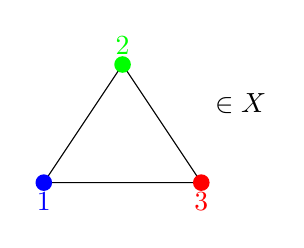
\begin{tikzpicture}
\draw (0,0) -- (1,1.5) -- (2,0) -- cycle;
\fill[blue] (0,0) circle (3pt) node[anchor = north] {$1$};
\fill[green] (1,1.5) circle (3pt) node[anchor = south] {$2$};
\fill[red] (2,0) circle (3pt) node[anchor = north] {$3$};
\node at (2.5,1) {$\in X$};
\end{tikzpicture}
\end{figure}
Знайдемо кількість орбіт $|X/_{D^3}|$ за допомогою леми Бернсайда.
\bigskip \\
Опишемо для початку всі можливі множини нерухомих точок:
\begin{align*}
\Fix_{D_3}(e) = X ; \\
\Fix_{D_3}(r) = \Fix_{D_3}(r^2) = \{ \text{трикутник } \in X \mid 1 = 2 = 3 \}; \\
\Fix_{D_3}(s) = \{ \text{трикутник } \in X \mid 2 = 3 \}; \\
\Fix_{D_3}(sr) = \{ \text{трикутник } \in X \mid 1 = 3 \}; \\
\Fix_{D_3}(sr^2) = \{ \text{трикутник } \in X \mid 1 = 2 \}.
\end{align*}
Тоді одержимо наступне:
\begin{align*}
|X/_{D^3}| = \dfrac{1}{6} (27 + 3 + 3 + 9 + 9 + 9) = 10.
\end{align*}
Насправді, $|X/_{D^3}|$ дає відповідь на питання, скільки різних способів зафарбувати вершини трикутника з точністю до його руху.
\end{example}

\begin{example}
Якщо $H \leq G$ (\textit{скінченна підгрупа}) та $H$ діє на множину $G$ множенням ліворуч, то зауважимо, що $\Stab_H(g) = \{e\}$, звідси за лемою Бернсайда\footnote{Приклад, який типу мотивує, чому кількість орбіт ми позначаємо саме так. Проте мені особисто більше подобається інша мотивація цього позначення, але для цього треба знання топологічних просторів, щоб пояснити.}
\[
|G/_H| = \dfrac{1}{|H|} \sum_{g \in G} |\Stab_G(g)| = \dfrac{1}{|H|} \sum_{g \in G} 1 = \dfrac{|G|}{|H|}.
\]
\end{example}

\begin{remark}
Для нескінченної групи $G$ формула з леми Бернсайда вже не працює.
\bigskip \\
Зокрема якщо $G$ --- нескінченна група, то, розглядаючи дію групи на себе, одержимо, що $|G/_G| = 1$. При цьому $\Stab_G(x) = \{e\}$, тому в формулі Бернсайда виникне невизначеність $\dfrac{\infty}{\infty}$.
\end{remark}
\newpage

%end Теорія групової дії
%\fi

\section{Ряди підгруп}
\subsection{Комутанти}
\begin{definition}
Нехай $\left<G,*\right>$ --- група та $x,y \in G$.\\
\textbf{Комутатором $x,y$} назвемо об'єкт
\begin{align*}
[x,y] = x*y*x^{-1}*y^{-1}.
\end{align*}
\end{definition}

\begin{proposition}[Властивості комутаторів]
Нехай $\left< G,* \right>$ --- група. Тоді справедливе наступне:
\begin{enumerate}[nosep,wide=0pt,label={\arabic*)}]
\item $x*y = [x,y]*(y*x)$;
\item $x,y$ комутують між собою $\iff [x,y] = e$;
\item $[x,y]^{-1} = [y,x]$;
\item $\forall g \in G: [x^g,y^g] = [x,y]^g$ (\textit{нагадую, під $x^g$ мається на увазі спряження});
\item Нехай $\left< H,\star\right>$ --- ще одна група та $\varphi \colon G \to H$ --- гомоморфізм груп. Тоді $\varphi([x,y]) = [\varphi(x),\varphi(y)]$.
\end{enumerate}
(\textit{вправа: довести всі ці властивості})
\end{proposition}

\iffalse %exercise
\begin{proof}
\begin{enumerate}[topsep=0pt,wide=0pt,label={\arabic*)}]
\item Доводиться в один рядок:
\[ 
x*y = x*y*\textcolor{red}{x^{-1}*y^{-1}*y*x} = [x,y]*y*x.
\]
\item Якщо $x,y$ комутують, тобто $x*y=y*x$, то звідси 
\[
[x,y] = x*y*x^{-1}*y^{-1} = y*x*x^{-1}*y^{-1} = e.
\]
Якщо $[x,y] = e$, тобто $x*y*x^{-1}*y^{-1} = e$, то звідси $x*y = y*x$.

\item Також доводиться в один рядок: 
\[
[x,y]^{-1} = (x*y*x^{-1}*y^{-1})^{-1} = y*x*y^{-1}*x^{-1} = [y,x].
\]
\item Тут вже треба трохи подовше:
\begin{align*}
[x^g,y^g] & = x^g*y^g*(x^g)^{-1}*(y^g)^{-1} \\
& = (g^{-1}*x*g)*(g^{-1}*y*g)*(g^{-1}*x^{-1}*g)*(g^{-1}*y^{-1}*g) \\
& = g^{-1}*(x*y*x^{-1}*y^{-1})*g = g^{-1}*[x,y]*g = [x,y]^g.
\end{align*}

\item Тут теж подовше, але водночас не насткільки багато:
\begin{gather*}
\varphi([x,y]) = \varphi(x*y*x^{-1}*y^{-1}) = \varphi(x) \star \varphi(y) \star \varphi(x^{-1}) \star \varphi(y^{-1}) \\ 
= \varphi(x) \star \varphi(y) \star (\varphi(x))^{-1} \star (\varphi(y))^{-1} = [\varphi(x),\varphi(y)]. \qedhere
\end{gather*}
\end{enumerate}
\end{proof}
\fi

\begin{remark}
Перша властивість каже, що комутатор $x,y$ --- це типу коректуючий множник, що дозволяє переставляти $x,y$ місцями.
\end{remark}

\begin{definition}
Нехай $\left<G,*\right>$ --- група.\\
\textbf{Комутантом} (або \textbf{похідною}) групи $G$ називають підгрупу
\begin{align*}
G' = \left< [x,y] \mid x \in G, y \in G \right>.
\end{align*}
(\textit{іншими словами, це --- підгрупа, породжена комутаторами}).
\end{definition}

\begin{remark}
Ми знаємо, що в породжуючих елементах там фігурує добуток елементів, деякі з них є оборотними. Але за властивістю 3) оборотний до комутатора --- теж комутатор. Внаслідок цього можна записати 
\[
G' = \{ [x_1,y_1]*\dots*[x_n,y_n] \mid x_i,y_i \in G, n \in \mathbb{N} \}.
\]
\end{remark}

\begin{remark}
Принципово, що комутатори породжують підгрупу. Якщо залишити просто множину комутаторів, то вона вже не буде підгрупою, оскільки порушується замкненість.
\bigskip \\
Зокрема розглянемо $\mathrm{SL}_2(\mathbb{R})$. Нижче буде доведено, що $(\mathrm{SL}_2(\mathbb{R}))' = \mathrm{SL}_2(\mathbb{R})$. Серед них
\[ 
-I = \begin{pmatrix}
-1 & 0 \\
0 & -1
\end{pmatrix}
\]
не розписується як комутатор двох матриць в даній групі. Із іншого боку, $-I \in \mathrm{SL}_2(\mathbb{R}))'$, тому записується як добуток комутаторів. Оскільки $-I$ не належить множині комутаторів, то порушується замкненість відносно множення в множині всіх комутаторів, тому це не підгрупа.
\end{remark}

\begin{remark}
Справедливе наступне:
\begin{center}
$G$ --- абелева група $\iff G' = \{e\}$.
\end{center}
Отже, комутант --- це така собі міра неабелевості груп.
\end{remark}

\begin{example}
Доведемо, що $(S_n)' = A_n$ (\textit{але перед цим ознайомтеся з \lmref{A_n_is_generated_by_3_cycles}}).
\bigskip \\
Зазначимо, що $[\sigma,\tau] = \sigma \tau \sigma^{-1} \tau^{-1}$ завжди парна перестановка, оскільки $\sigma, \sigma^{-1}$ мають однакову парність (\textit{так само й $\tau, \tau^{-1}$}). Отже, $S_n' \subset A_n$.\\
Із іншого боку, при $n \geq 3$ відомо, що $A_n$ породжується $3$-циклами. Кожен $3$-цикл подамо в такому вигляді:
\[
(ijk) = (ij)(ik)(ij)(ik) = (ij)(ik)(ij)^{-1}(ik)^{-1} = [(ij),(ik)] \in S_n'.
\]
Отже, отримаємо $A_n \subset S_n'$ (\textit{навіть при $n \in \{1,2\}$ це працює}).
\end{example}

%exercise
\iffalse
\begin{example}
Доведемо, що $Q'_8 = \{-1,1\}$.
\bigskip \\
Уже відомо, що $Z(Q_8) = \{1,-1\}$. Тому залишилося подивитися на комутанти $[x,y]$, коли 
\[
x,y \in \{\pm i, \pm j, \pm k\}.
\]
Спочатку розглянемо комутант $[i,j]$, тоді
\[
[i,j] = iji^{-1}j^{-1} = k (-k)^{-1} = k^2 = -1.
\]
Аналогічно можна переконатися, що 
\[
[j,k] = [k,i] = -1.
\]
(\textit{автоматично знайшли $[j,i], [k,j], [i,k]$}). Інші комутанти перевіряються аналогічно. Отже, в нас всі комутанти $1$ або $-1$ (\textit{тому й добуток теж}). Значить, $Q_8' = \{-1,1\}$.
\end{example}
\fi

%exercise
\iffalse
\begin{example}
Знайдемо комутатор групи 
\[
G = \left\{ \begin{pmatrix}
1 & a & 0 \\
0 & 1 & 0 \\
0 & b & c
\end{pmatrix} \Big| a,b,c \in \mathbb{R}, c \neq 0 \right\}
\] 
(\textit{вправа: переконатися, що $G$ буде підгрупою $\mathrm{GL}_3(\mathbb{R})$}).\\
Розглянемо комутатор довільних двох матриць
\[
\left[ \begin{pmatrix}
1 & a & 0 \\
0 & 1 & 0 \\
0 & b & c
\end{pmatrix},
\begin{pmatrix}
1 & x & 0 \\
0 & 1 & 0 \\
0 & y & z
\end{pmatrix}
\right] \overset{\textit{(вправа: перевірити)}}{=} \begin{pmatrix}
1 & 0 & 0 \\
0 & 1 & 0 \\
0 & -bz+b+cy-y & 1
\end{pmatrix} = \begin{pmatrix}
1 & 0 & 0 \\
0 & 1 & 0 \\
0 & \xi & 1
\end{pmatrix}.
\]
Таким чином, кожен комутант --- одинична матриця, але на третьому рядку та другому стовпчику розташоване число. Множення таких матриць приведе до матриці такої ж форми. Отже, 
\[
G' \subset \left\{ \begin{pmatrix}
1 & 0 & 0 \\
0 & 1 & 0 \\
0 & \xi & 1
\end{pmatrix} \Big| \xi \in \mathbb{R} \right\}.
\]
Із іншого боку, погравшись трошки, отримаємо, що
\[
\begin{pmatrix}
1 & 0 & 0 \\
0 & 1 & 0 \\
0 & \xi & 1
\end{pmatrix} = \left[ \begin{pmatrix}
1 & 0 & 0 \\
0 & 1 & 0 \\
0 & -2\xi & 2
\end{pmatrix}, \begin{pmatrix}
1 & 0 & 0 \\
0 & 1 & 0 \\
0 & -\xi & 2
\end{pmatrix} \right],
\]
тобто кожна матриця такого типу розписується як комутатор. Значить, \[
\left\{ \begin{pmatrix}
1 & 0 & 0 \\
0 & 1 & 0 \\
0 & \xi & 1
\end{pmatrix} \Big| \xi \in \mathbb{R} \right\} \subset G'.
\]
Звідси отримаємо 
\[
G'= \left\{ \begin{pmatrix}
1 & 0 & 0 \\
0 & 1 & 0 \\
0 & \xi & 1
\end{pmatrix} \Big| \xi \in \mathbb{R} \right\}.
\]
\end{example}
\fi

\begin{proposition}
Нехай $\left< G, *\right>, \left<H,\star \right>$ --- групи та $\varphi \colon G \to H$ --- гомоморфізм. Тоді $\varphi(G') \leq H'$. Ба більше, якщо $\varphi$ --- сюр'єктивний, то $\varphi(G') = H'$.
\end{proposition}

\begin{proof}
\begin{enumerate}[wide=0pt,topsep=0pt,label={\Roman*.}]
\item $\varphi(G') \leq H'$.\\
Нехай $u,v \in \varphi(G')$, тобто для них існують елементи $a,b \in G'$, для яких $\varphi(a) = u, \varphi(b) = v$. Але оскільки $a,b \in G'$, то тоді 
\[
a = [x_1,y_1]* \dots *[x_n,y_n],\quad b = [w_1,z_1]* \dots *[w_m, z_m]
\]
при $x_i,y_i,w_i,z_i \in G$. Із іншого боку, 
\[
u = [\varphi(x_1),\varphi(y_1)]* \dots *[\varphi(x_n),\varphi(y_n)],\quad v = \varphi([x_2,y_2]) = [\varphi(z_k), \varphi(w_k)]* \dots *[\varphi(z_1), \varphi(w_1)].
\]
Звідси випливає, що 
\[
u \star v^{-1} = \varphi( [x_1,y_1] * \dots *[x_n,y_n] * [z_k,w_k] * \dots * [z_1,w_1] ) = \varphi(c)
\]
при деякому елементі $c \in G'$. Отже, $u \star v^{-1} \in \varphi(G')$.

\item \textit{$\varphi(G') = H'$ за умови, що $\varphi$ --- сюр'єктивний}.\\
Нехай $h_1,h_2 \in H$, тобто звідси $\varphi(a) = h_1, \varphi(b) = h_2$ для деяких $a,b \in G$. Отже, 
\[
\varphi([a,b]) = [\varphi(a),\varphi(b)] = [h_1,h_2] \in \varphi(G').
\]
Якщо взяти елемент $u \in H'$, то це буде добуток комутаторів, кожний з яких потрапляє уже в $\varphi(G')$. Отже, $u \in G'$. Отримали $\varphi(G') = H'$. \qedhere
\end{enumerate}
\end{proof}

\begin{definition}
Нехай $\left<G,*\right>$ --- група та $K,H \leq G$.\\
\textbf{Взаємним комутантом} назвемо таку підгрупу:
\begin{align*}
[K,H] = \left< [x,y] \mid x \in K, y \in H \right>.
\end{align*}
\end{definition}

\begin{remark}
$[K,K] = K'$. (\textit{відповідно ми можемо писати $[G,G] = G'$ для кожної групи} $G$\footnote{До речі, таке позначення $[G,G]$ є загально прийнятим в західній літературі.}).
\end{remark}

\begin{proposition}
Нехай $K \triangleleft G$. Тоді $K' \triangleleft G$.
\end{proposition}

\begin{proof}
Нехай $k \in K'$ та $g \in G$, тобто маємо 
\[
k = [u_1,v_1]* \dots *[u_n,v_n],
\]
причому $u_i,v_i \in K$. Тоді
\[
g*k*g^{-1} = g*[u_1,v_1]*g^{-1}*g*[u_2,v_2]*g^{-1}*\dots*g*[u_n,v_n]*g^{-1}.
\]
Отже, достатньо показати, що
\[
g*[u_1,v_1]*g^{-1} = [u_1,v_1]^g = [u_1^g,v_1^g] \in K.
\]
Так воно й буде, оскільки $u_1^g,v_1^g \in K$ в силу $K \triangleleft G$. Внаслідок цього доведемо $g*k*g^{-1} \in K'$.
\end{proof}

\begin{corollary}
$G' \triangleleft G$.
\end{corollary}

\begin{theorem}[Основна теорема про комутанти]
Нехай $\left<G,*\right>$ --- група. Тоді
\begin{enumerate}[nosep,wide=0pt,label={\arabic*)}]
\item $G/_{G'}$ --- абелева група;
\item $H \triangleleft G$, причому $G/_H$ --- абелева $\iff G'$ --- підгрупа $H$, що уже є підгрупою $G$ (\textit{тобто $H$ --- проміжкова підгрупа між $G',G$}).
\end{enumerate}
\end{theorem}

\begin{proof}
\begin{enumerate}[topsep=0pt,wide=0pt,label={\arabic*)}]
\item (\textit{звісно, є більш прямолійнійний варіант доведення, але хочеться показати, як вивести абелевість за допомогою властивості 2).}) \\
Розглянемо проєкцію $\pi \colon G \to G/_{G'}$, де відомо, що $\ker \pi = G'$. Оберемо $x*G',\ y*G' \in G/_{G'}$. Тоді
\[
[x*G',y*G'] = [\pi(x), \pi(y)] = \pi([x,y]) \overset{[x,y] \in G' = \ker \pi}{=} e*G'.
\]
За властивістю 2) одержимо
\[
(x*G')*(y*G') = (y*G')*(x*G').
\]

\item Доведення буде в обидві сторони.\\
\rightproof Дано: $H \triangleleft G$, причому $G/_H$ --- абелева.\\
Розглянемо деякий комутатор $[a,b] \in G'$, тоді звідси $[a*H,b*H] = e*H = H$, просто тому що $G/_H$ --- абелева. Але із іншого боку, $[a*H,b*H] = [a,b]*H$, тож ми одержимо $[a,b] \in H$. Отже, ми отримали, що всі комутатори потрапляють в $H$. Множина $G'$ породжується комутаторами не просто в $G$, а тепер у $H$. Таким чином, $G'$ --- підгрупа $H$.
\bigskip \\
\leftproof Дано: $G'$ --- підгрупа $H$.\\
Нехай $x \in G$ та $y \in H$. Тоді зауважимо, що комутатор $[x,y] \in G' \subset H$, тобто $x*y*x^{-1}*y^{-1} \in H$. Однак оскільки $y \in H$, то тоді $x*y*x^{-1} \in H$. Значить, $H \triangleleft G$.\\
Крім того, маємо наступне:
\[
a*H,b*H \in G/_H \implies [a*H,b*H] = [a,b]*H.
\]
Але $[a,b] \in G' \subset H$ за умовою, тож $[a*H,b*H] = e*H = H$. Тобто $a*H,b*H$ комутують між собою. Значить, $G/_H$ буде дійсно абелевою. \qedhere
\end{enumerate}
\end{proof}

\begin{corollary}
$G'$ --- найменша нормальна підгрупа $G$, для якої $G/_{G'}$ --- абелева.
\end{corollary}

\begin{example}
Доведемо, що $D_n' = \left<r^2\right>$.
\bigskip \\
Зауважимо, що $r^{2k} = [r^k,s]$, тож звідси випливає, що $\left<r^2\right> \subset D_n'$.\\
Із іншого боку, $\left< r^2 \right> \triangleleft D_n$, при цьому $D_n/_{\left<r^2\right>}$ буде абелевою, оскільки його порядок або $2$, або $4$ в залежності від парності $n$-кутника. Отже, за основною теоремою про комутанти $D_n' \subset \left< r^2 \right>$.
\end{example}

\begin{example}
Доведемо, що $(\mathrm{GL}_n(\mathbb{R}))' = \mathrm{SL}_n(\mathbb{R})$\footnote{Насправді кажучи, якщо взяти поле $k$, то також справедливе $(\mathrm{GL}_n(k))' = \mathrm{SL}_n(k)$, окрім випадка, коли одночасно $n =2$ та $|k| = 2$. Доведення повторюється.}.
\bigskip \\
Пригадаємо, що ${\mathrm{GL}_n(\mathbb{R})}/_{\mathrm{SL}(\mathbb{R})} \cong \mathbb{R} \setminus \{0\}$, причому остання група абелева, тобто факторгрупа ${\mathrm{GL}_n(\mathbb{R})}/_{\mathrm{SL}(\mathbb{R})}$ --- абелева. Отже, $(\mathrm{GL}_n(\mathbb{R}))' \subset \mathrm{SL}_n(\mathbb{R})$.
\bigskip \\
Далі, із \exref{SL_n_is_generated_by_row_addition_matrices} відомо, що кожна матриця $A \in \mathrm{SL}_n(\mathbb{R})$ записується як добуток елементарних матриць вигляду $E_{i \to i+\lambda j}$. Тут існують дві можливості:
\begin{itemize}[wide=0pt]
\item $n \geq 3$.\\
Зауважимо, що справедливе наступне (\textit{вправа: переконатися самостійно}):
\[
[E_{i \to i+\alpha k},\ E_{k \to k+\beta j}] = E_{i \to i + (\alpha \beta) \cdot j}.
\]
Тому звідси випливає, що якщо в нас є матриця $E_{i \to i + \lambda j}$ в розкладі, то можна підібрати числа $\alpha,\beta \in \mathbb{R}$, а також в силу $n \geq 3$ --- деяке число $k \notin \{i,j\}$, аби виконувалась рівність $[E_{i \to i+\alpha k},\ E_{k \to k+\beta j}] = E_{i \to i+\lambda j}$. Значить, $A \in (\mathrm{GL}_n(\mathbb{R}))'$.

\item $n = 2$.\\
Зауважимо, що справедливе наступне:
\[
\left[ \begin{pmatrix}
1 & \alpha \\
0 & 1
\end{pmatrix},\ \begin{pmatrix}
\beta & 0 \\
0 & \gamma
\end{pmatrix} \right] = \begin{pmatrix}
1 & \alpha \left( 1- \dfrac{\beta}{\gamma} \right) \\
0 & 1
\end{pmatrix}.
\]
Тому звідси випливає, що якщо в нас є матриця $E_{1 \to 1 + \lambda 2}$ в розкладі, то можна підібрати таке $\alpha,\beta,\gamma$, щоб виконувалось $\lambda = \alpha \left(1 - \dfrac{\beta}{\gamma}\right)$, аби виконувалась рівність вище. Отже, $E_{1 \to 1 + \lambda 2} \in (\mathrm{GL}_2(\mathbb{R}))'$. Аналогічно $E_{2 \to 2 + \lambda 1} \in (\mathrm{GL}_2(\mathbb{R}))'$ (\textit{якщо взяти $\gamma = 1/\beta$, то навіть можна добитися того, що елементарні матрицю потраплять в $(\mathrm{SL}_2(\mathbb{R}))'$}).
\end{itemize}
У результаті чого $\mathrm{SL}_n(\mathbb{R}) \subset (\mathrm{GL}_n(\mathbb{R}))'$ при будь-якому $n \geq 1$.
\end{example}

\begin{example}
Із попереднього прикладу навіть одержали, що $(\mathrm{SL}_n(\mathbb{R}))' = \mathrm{SL}_n(\mathbb{R})$\footnote{Знову ж таки, навіть більше можна сказати. Якщо $k$ --- знову поле, то $(\mathrm{SL}_n(k))' = \mathrm{SL}_n(k)$, окрім випадка, коли одночасно $n = 2$ та $|k| \leq 3$. До речі, $\mathrm{SL}_n(\mathbb{R})$ є прикладом так званої \textbf{досконалої групи} (англійською \textbf{perfeсt group}), оскільки виконується рівність $G' = G$. Найменшою нетривіальною досконалою групою є група $A_5$.}.
\end{example}

\begin{remark}
Із групи $G$ ми отримали нову абелеву групу $G/_{[G,G]}$. Цей процес називається \textbf{абеліанізацією} та часто позначають цю групу за $G_{\text{ab}}$.
\end{remark}

\begin{example}
Зокрема маємо групу $S_n$, знайдемо його абеліанізацію $(S_n)_{\text{ab}}$. Дійсно,
\[
(S_n)_{\text{ab}} = {S_n}/_{S_n'} = {S_n}/_{A_n} \cong \mathbb{Z}_2.
\]
\end{example}

\iffalse
\begin{example}
Абеліанізуємо групу кватерніонів $Q_8$.
\[
{Q_8}/_{Q_8'} = {Q_8}/_{\{-1,1\}} \cong \mathbb{Z}_4 \cong \mathbb{Z}_2 \times \mathbb{Z}_2.
\]
\end{example}
\fi

\subsection{Композиційний ряд}
\begin{definition}
Нехай $G$ --- група.\\
\textbf{Рядом} підгруп $G_i$ групи $G$ називають спадну послідовність підгруп
\begin{align*}
G = G_0 \supsetneq G_1 \supsetneq G_2 \supsetneq \dots
\end{align*}
\textbf{Довжиною ряда} назвемо кількість строгих вкладень.
\end{definition}

\begin{definition}
Нехай $G$ -- група та $G = G_0 \supsetneq G_1 \supsetneq G_2 \supsetneq \dots$ --- ряд підгруп $G$.\\
Даний ряд називається \textbf{субнормальним}, якщо
\begin{align*}
G_i \triangleright G_{i+1}
\end{align*}
Фактормножини ${G_i}/_{G_{i+1}}$ називаються \textbf{композиційними множниками}.\\
Починаючи з субнормального ряду, можна визначати довжину цього ряду.
\end{definition}

\begin{remark}
Уже відомо, що якщо умовно $G_1 \triangleleft G_1$ та $G_1 \triangleleft G_0$, то зовсім не обов'язково, щоб було $G_2 \triangleleft G_0$. Тому субнормальний ряд я не можу позначити за $G = G_0 \triangleright G_1 \triangleright G_2 \triangleright \dots$. Коректніше в нашому випадку буде писати $G = G_0 \supsetneq G_1 \supsetneq G_2 \supsetneq \dots$ при $G_i \triangleright G_{i+1}$.
\end{remark}

\begin{definition}
Нехай $G$ -- група та $G = G_0 \supsetneq G_1 \supsetneq G_2 \supsetneq \dots$ --- ряд підгруп $G$.\\
Даний ряд називається \textbf{нормальним}, якщо
\begin{align*}
G \triangleright G_{i}.
\end{align*}
\end{definition}

\begin{remark}
Оскільки $G \triangleright G_i$ при всіх можливих $i$, то тоді $G_i \triangleright G_{i+1}$, тому нормальний ряд автоматично субнормальний. Також в цьому випадку можна ряд позначати 
\[
G = G_0 \triangleright G_1 \triangleright G_2 \triangleright \dots
\]
\end{remark}

\begin{remark}
Деякі автори субнормальні ряди називають просто нормальними. Я вирішив відокремити різницю, аби не було плутанини.
\end{remark}

\begin{remark}
Справедливе наступне для субнормальних рядів:
\begin{itemize}[nosep,wide=0pt]
\item Ряд групи $G$ має нульову максимальну довжину $\iff G$ --- тривіальна група.

\item Ряд групи $G$ має одиничну максимальну довжину $\iff G$ --- нетривіальна проста група.
\end{itemize}
Отже, довжина ряду $G$ визначає, наскільки далеко від властивості простоти знаходиться група $G$.
\end{remark}

\begin{definition}
Нехай $G$ --- група та $G = G_0 \supsetneq G_1 \supsetneq G_2 \supsetneq \dots \supsetneq G_n = \{e\}$ при $G_i \triangleright G_{i+1}$ --- скінченний субнормальний ряд.\\
Даний ряд називається \textbf{композиційним рядом}, \iffalse\footnote{Композиційний ряд, за означенням, має скінченну довжину, хоча існує нескінченний ряд, який задовольняє умову того, що композиційні множники --- прості. Зокрема можна взяти групу $p$-адичних чисел $\left<\mathbb{Z}_p,+\right>$ та розглянути ось такий ланцюг:
\[
\mathbb{Z}_p \triangleright p \mathbb{Z}_p \triangleright p^2 \mathbb{Z}_p \triangleright \dots
\]
(\textit{група $\mathbb{Z}_p$ абелева, тому буде нормальний ряд}). Треба знати, що $p^i \mathbb{Z}_p/_{p^{i+1} \mathbb{Z}_p} \cong \mathbb{Z}/_{p\mathbb{Z}}$, де остання група проста.
}\fi якщо
\begin{align*}
G_i/_{G_{i+1}} \text{ --- прості групи.}
\end{align*}
(\textit{тобто всі композиційні множники є простими групами})
\end{definition}

\begin{proposition}
Нехай $G$ --- скінченна група. Тоді $G$ має композиційний ряд.
\end{proposition}

\begin{proof}
Доведемо це твердження за МІ за $|G|$.
\begin{enumerate}[nosep,wide=0pt,label={\Roman*.}]
\item \textit{База індукції}. $|G| = 1$ --- це тривіальна група, тут все ясно.

\item \textit{Припущення індукції}. Твердження виконується для деякого порядка, меншого за $|G|$.

\item \textit{Крок індукції}. Нехай група має порядок $|G|$. Якщо $G$ --- проста група, то знайшли (\textit{див.\ зауваження вище}). Інакше існує нетривіальна нормальна підгрупа $H \triangleleft G$ (\textit{оберемо $H$ максимального можливого порядку: чому це так можливо, думаю, це зрозуміло}). За припущенням МІ група $H$ має композиціний ряд
\[ 
H = H_0 \supsetneq H_1 \supsetneq \dots \supsetneq H_k = \{e\},
\] 
причому кожен композиційний множник ${H_i}/_{H_{i+1}}$ --- проста група. Тоді зазначимо, що 
\[
G \supsetneq H = H_0 \supsetneq  H_1 \supsetneq \dots \supsetneq H_k = \{e\}
\]
буде композиційним рядом, причому $G/_H$ --- теж проста (\textit{в силу максимальності}).
\end{enumerate}
МІ доведено.
\end{proof}

% overcomplicated
\iffalse
\begin{remark}
Існування максимальної нормальної підгрупи можна строго описати за допомогою леми Цорна. Нехай $G$ --- непроста група та $\mathcal{S}$ --- множина всіх нетривіальних нормальних власних підгруп $G$. Зрозуміло, що $\mathcal{S} \neq \emptyset$ (\textit{бо $G$ --- непроста}) та впорядковані за вкладенням, причому $G$ --- верхня межа $\mathcal{S}$.  
\end{remark}
\fi

\begin{remark}
Твердження не завжди працює у випадку нескінченної групи.
\end{remark}

% example of the preceding remark
\iffalse
\begin{example}
Доведемо, що $\mathbb{Z}$ не має взагалі композиційного ряду.
\bigskip \\
!Припустимо, що $\mathbb{Z}$ навпаки має композиційний ряд, тобто в нас ланцюг 
\[
\mathbb{Z} \supsetneq d_1 \mathbb{Z} \supsetneq d_2 \mathbb{Z} \supsetneq \dots \supsetneq d_n \mathbb{Z} = \{0\}
\]
(\textit{пригадаємо, що будь-яка підгрупа $\mathbb{Z}$ має вигляд $d \mathbb{Z}$ при деякому невід'ємному $d$, причому також відомо, що $d_2 \mathbb{Z} \leq d_1 \mathbb{Z} \iff d_1 \mid d_2$}). Оскільки всі ці підгрупи абелеві, то тоді в нас ряд автоматично нормальний. За умовою $d_{n-1} \mathbb{Z}$ --- проста, яка також циклічна, як підгрупа циклічної групи $\mathbb{Z}$, тобто $d_{n-1} \mathbb{Z} = \left<x\right>$. Але зауважимо, що $\left<x^2 \right> \triangleleft \left<x\right>$ --- суперечність! Бо в нас $d_{n-1} \mathbb{Z}$ мала бути простою.
\end{example} 
Да й взагалі-то кажучи, справедливе ось таке твердження:
\fi

\begin{proposition}
Нехай $G$ --- абелева група. Тоді
\begin{center}
$G$ має композиційний ряд $\iff G$ --- скічненна.
\end{center}
(\textit{в один бік уже довели, залишилося довести в другий})
\end{proposition}

\begin{example}
Отже, зокрема $\mathbb{Z}$ взагалі не має композиційного ряду.
\end{example}

\begin{proof}
Припустимо, що абелева група $G$ має композиційний ряд:
\[
G = G_0 \triangleright G_1 \triangleright \dots \triangleright G_{n-1} \triangleright G_n = \{e\}.
\]
(\textit{у силу абелевості даний ряд буде нормальним}). Відомо, що $G_{n-1}$ --- проста група, тому має бути скінченною (\textit{якщо група нескінченна, вона має містити власну підгрупу, яка автоматично нормальна, але тоді перестане бути власною}). Далі візьмемо ввесь ряд та профакторизуємо по $G_{n-1}$ --- одержимо композиційний ряд
\begin{align*}
H = H_0 \triangleright H_1 \triangleright \dots \triangleright H_{n-1} = \{e\}
\end{align*}
(\textit{композиційні множники залишаються простими за ІІІ теоремою про ізоморфізм}). Аналогічними міркуваннями група $H_{n-2} = G_{n-2}/_{G_{n-1}}$ скінченна. Внаслідок чого тепер вже $G_{n-2}$ скінченна група. Далі візьмемо початковий ряд та профакторизуємо по $G_{n-2}$ --- і так далі.
\end{proof}

\begin{proposition}
Нехай $G$ --- група. Припустимо, що його субнормальний ряд має максимальну довжину (\textit{тобто іншого субнормального ряду більшої довжини нема}). Тоді даний ряд буде композиційним.
\end{proposition}

\begin{proof}
Маємо субнормальний ряд при $G_i \triangleright G_{i+1}$
\[
G = G_0 \supsetneq G_1 \supsetneq G_2 \supsetneq \dots \supsetneq G_n = \{e\},
\]
який має максимальну довжину.\\
!Припустимо, що даний субнормальний ряд --- не композиційний, тобто існує композиційний множник ${G_i}/_{G_{i+1}}$, який не є простим. Отже, існує нетривіальна власна підгрупа $K \triangleleft {G_i}/_{G_{i+1}}$. Підгрупі ставиться в відповідність підгрупа $G_{i+1} \triangleleft N \triangleleft G_i$. Таким чином, ми розширимо ряд 
\[
G = G_0 \supsetneq G_1 \supsetneq \dots \supsetneq G_i \supsetneq N \supsetneq G_{i+1} \supsetneq \dots \supsetneq G_n = \{e\},
\] 
який теж субнормальний --- суперечність за максимальністю!
\end{proof}

\begin{proposition}
Нехай $G$ --- група та $N \triangleleft G$ Тоді
\begin{center}
$G$ має композиційний ряд $\iff$ обидва $N,G/_N$ мають композиційні ряди.
\end{center}
\end{proposition}

\begin{proof}
\rightproof Дано: $G$ має композиційний ряд, скажімо
\[
G = G_0 \supsetneq G_1 \supsetneq G_2 \supsetneq \dots \supsetneq G_n = \{e\}.
\]
\begin{enumerate}[wide=0pt,label={\Roman*.}]
\item \textit{Існування композиційного ряду групи $N$}.\\
Перетнемо композиційний ряд групи $G$ з групою $N$ --- одержимо таку послідовність:
\[
N = G \cap N \supset G_1 \cap N \supset \dots \supset \{e\} \cap N = \{e\}.
\]
Причому $G_{i+1} \cap N \triangleleft G_i \cap N$. Якщо прибрати можливі повторення, то стверджується, що це формує композиційний ряд групи $N$. Для цього нам треба довести, що:
\begin{itemize}[nosep]
\item або ${G_i \cap N}/_{G_{i+1} \cap N}$ --- тривіальна група (\textit{тому $G_{i+1} \cap N = G_i \cap N$, отже включення $G_{i} \cap N \subset G_{i+1} \cap N$ можна прибрати});
\item або ${G_i \cap N}/_{G_{i+1} \cap N} \cong {G_i}/_{G_{i+1}}$ (\textit{тому ${G_i \cap N}/_{G_{i+1} \cap N}$ стане простою групою}).
\end{itemize}
Розглянемо гомоморфізм $G_i \cap N \xhookrightarrow{\imath} G_i \xtwoheadrightarrow{\pi} G_i/_{G_{i+1}}$. Його ядро дорівнює $G_{i+1} \cap N$. Тому за І теоремою ${G_i \cap N}/_{G_{i+1} \cap N} \cong \Im ( \pi \circ \imath) = \pi(G_i \cap N) = {G_i \cap N}/_{G_{i+1}}  \hookrightarrow G_i/_{G_{i+1}}$. Значить, ${G_i \cap N}/_{G_{i+1} \cap N}$ можна сприймати як підгрупу ${G_i}/_{G_{i+1}}$. Причому зазначимо, що ${G_i \cap N}/_{G_{i+1} \cap N} \triangleleft {G_i}/_{G_{i+1}}$ (\textit{бо $N \triangleleft G$}). Оскільки ${G_i}/_{G_{i+1}}$ --- проста, то ми довели, що треба було.

\item \textit{Існування композиційного ряду $G/_N$}.\\
Цього разу розглянемо ось таку послідовність (\textit{помножимо чисельник та знаменник на $N$}):
\[ 
G/_N \supset {G_1N}/_N \supset {G_2N}/_N \supset \dots \supset {\{e_G\} N}/_N = \{e_{G/_N}\}.
\]
Причому ${G_{i+1}N}/_N \triangleleft {G_i N}/_N$, оскільки $G_{i+1}N \triangleleft G_1 N$ (\textit{а це виконується, тому що $N \triangleleft G$}).
\iffalse
Якщо детальніше, нехай $x \in G_i N$ та $y \in G_{i+1}N$, тоді елемент $xyx^{-1} = g_in_1 g_{i+1}n_2 n_1^{-1} g_1^{-1} \in N \subset GN$.
\fi
Аналогічно тому, як було вище, нам залишилося довести, що або ${{G_i N}/_N}/_{{G_{i+1}N}/_N}$ --- тривіальний або ${{G_i N}/_N}/_{{G_{i+1}N}/_N} \cong {G_i}/_{G_{i+1}}$.\\
За ІІІ теоремою про ізоморфізм ${{G_i N}/_N}/_{{G_{i+1}N}/_N} \cong {G_i N}/_{G_{i+1} N}$. Цього разу розглянемо гомоморфізм $G_i \hookrightarrow G_i N \twoheadrightarrow {G_i N}/_{G_{i+1}N}$, який є сюр'єктивним. Підгрупа $G_{i+1} \subset \ker$ нашого гомоморфізму. Отже, існує сюр'єктивний гомоморфізм ${G_i}/_{G_{i+1}} \twoheadrightarrow {G_i}/_{\ker} \cong {G_iN}/_{G_{i+1}N}$. Оскільки ${G_i}/_{G_{i+1}}$ --- проста, то образ також буде простим (\textit{в принципі, неважко показати}), тож звідси ${G_iN}/_{G_{i+1}N}$ або тривіальна, або ${G_iN}/_{G_{i+1}N} \cong {G_i}/_{G_{i+1}}$.
\end{enumerate}

\leftproof Дано: $N,G/_N$ мають композиційні ряди. Запишемо їх:
\[
G/_N \supsetneq {\tilde{N}_1}/_N \supsetneq {\tilde{N}_2}/_N  \supsetneq \dots \supsetneq \{e_{G/_N}\}, \qquad N \supsetneq N_1 \supsetneq N_2 \supsetneq \dots \supsetneq \{e\}.
\]
За теоремою про відповідність $\tilde{N}_1$ --- підгрупа $G$, $\tilde{N}_2$ --- підгрупа $\tilde{N_1}$ тощо, але всі $\tilde{N}_i \supset N$. Тобто маємо ось такий ланцюг:
\[
G \supsetneq \tilde{N}_1 \supsetneq \tilde{N}_2 \supsetneq \dots \supsetneq N \supsetneq N_1 \supsetneq N_2 \supsetneq \dots \supsetneq \{e\}. \qedhere
\]
\end{proof}

\begin{corollary}
Довижна композиційного ряду $G$ дорівнює сумі довжин композиційних рядів $N$ та $G/_N$. Композиційні множники $G$ складаються з набору композиційних множників $N$ та $G/_N$.
\end{corollary}

\iffalse
\begin{remark}
Якщо група $G$ має композиційний ряд, а $H \triangleleft G$ (\textit{не обов'язково нормальна підгрупа}), то $H$ також має композиційний ряд. Якщо $G$ --- скінченна група, то $H$ також скінченна, тому композиційний ряд і для нього існує. Якщо $G$ --- нескінченна, то $G$ --- абелева, а тому $H$ також абелева, тому композиційний ряд існує.
\end{remark}
\fi

\subsection{Лема метелика}
\begin{lemma}
Нехай $G$ --- група, $H_1,H_2 \leq G$ та $N_1 \triangleleft H_1,\ N_2 \triangleleft H_2$. Тоді
\begin{align*}
\dfrac{N_1 (H_1 \cap H_2)}{N_1(H_1 \cap N_2)} \cong \dfrac{H_1 \cap H_2}{(H_1 \cap N_2) (N_1 \cap H_2)} \cong \dfrac{N_2(H_1 \cap H_2)}{N_2(N_1 \cap H_2)}.
\end{align*}
\end{lemma}

\begin{proof}
Нам досить довести перший ізоморфізм в силу симетрії. І перш ніж доводити ізоморфність, нам варто переконатися, що такі групи, взагалі-то кажучи, визначені.

\begin{enumerate}[wide=0pt,label={\Roman*.}]
\item $N_1 (H_1 \cap N_2) \triangleleft N_1(H_1 \cap H_2)$.\\
Нехай $u \in N_1(H_1 \cap H_2)$ та $\xi \in N_1(H_1 \cap N_2)$, тобто маємо
\[
u = h_{12} \tilde{n}, \qquad \xi = \tilde{\tilde{n}} k
\]
для $\tilde{n}, \tilde{\tilde{n}} \in N_1,\ h_{12} \in H_1 \cap H_2,\ k \in H_1 \cap N_2$. Зазначимо, що елемент $u$ записаний в такому порядку, просто тому що $N_1(H_1 \cap H_2) = (H_1 \cap H_2) N_1$, адже $N_1 \triangleleft H_1$ та $H_1 \cap H_2 \leq H_1$. Далі,
\[
u \xi u^{-1} = h_{12} \tilde{n} \tilde{\tilde{n}} k \tilde{n}^{-1} h_{12}^{-1} = \left( h_{12} \tilde{n} \textcolor{red}{h_{12}^{-1}} \right) \left( \textcolor{red}{h_{12}} \tilde{\tilde{n}} k \tilde{n}^{-1} \textcolor{red}{k^{-1} h_{12}^{-1}} \right) \left( \textcolor{red}{h_{12} k} h_{12}^{-1} \right).
\]
Оскільки $N_1 \triangleleft H_1$, то елемент $h_{12} \tilde{n} h_{12}^{-1} \in N_1$. Також $s = k \tilde{n}^{-1} k^{-1} \in N_1$, а тому звідси $h_{12} \tilde{\tilde{n}} k \tilde{n}^{-1} k^{-1} h_{12}^{-1} = h_{12} s h_{12}^{-1} \in N_1$. Нарешті, оскільки $N_2 \triangleleft H_2$, то елемент $h_{12} k h_{12}^{-1} \in N_2 \cap H_1$. Отже, висновок:
\[
u \xi u^{-1} \in N_1 (N_2 \cap H_1).
\]

\item $(H_1 \cap N_2) (N_1 \cap H_2) \triangleleft H_1 \cap H_2$.\\
Нехай $u \in H_1 \cap H_2$ та $v \in (H_1 \cap N_2)(N_1 \cap H_2)$, тобто маємо $v = ab$ при $a \in H_1 \cap N_2,\ b \in N_1 \cap H_2$. Тоді
\[
uvu^{-1} = uabu^{-1} = (uau^{-1})(ubu^{-1}).
\]
За умови леми одержимо, що $uau^{-1} \in H_1 \cap N_2$ та $ubu^{-1} \in N_1 \cap H_2$. Отже,
\[
uvu^{-1} \in (H_1 \cap N_2)(N_1 \cap H_2).
\]

\item $\dfrac{N_1 (H_1 \cap H_2)}{N_1(H_1 \cap N_2)} \cong \dfrac{H_1 \cap H_2}{(H_1 \cap N_2) (N_1 \cap H_2)}$.\\
Позначимо $H = H_1 \cap H_2$ та $N = N_1(H_1 \cap N_2)$ та застосуємо ІІ теорему про ізоморфізм:
\[
\dfrac{N_1(H_1 \cap N_2)(H_1 \cap H_2)}{N_1(H_1 \cap N_2)} = \dfrac{NH}{N} \cong \dfrac{H}{H \cap N} = \dfrac{H_1 \cap H_2}{H_1 \cap H_2 \cap N_1(H_1 \cap N_2)}.
\]
Для завершення доведення варто лише зауважити наступне:
\[
N_1 (H_1 \cap N_2)(H_1 \cap H_2) = N_1(H_1 \cap H_2), \qquad H_1 \cap H_2 \cap N_1(H_1 \cap N_2) = (H_1 \cap N_2)(N_1 \cap H_2). \qedhere
\]
\end{enumerate}
\end{proof}

\begin{remark}
Цю лему ще називають \textbf{лемою Цассенгауса}. Альтернативна назва ''метелик'' виникла невипадково, адже ми можемо побудувати ось таку діаграму, яка дійсно нагадує метелик (\textit{ну я старався його намалювати}). Тут вища група є підгрупою нижньою (\textit{наприклад, $N_1 \cap H_2 \leq N_1$}).
\begin{figure}[H]
\centering
\adjustbox{scale=0.75,center}{%
\begin{tikzcd}
H_1 \cap N_2 \arrow[dash, rrrd, bend left=30] \arrow[dash, rdd, bend right=30] & & & & & & N_1 \cap H_2 \arrow[dash, ldd, bend left=30] \arrow[dash, llld, bend right=30] \\ %swap
 & & & (H_1 \cap N_2)(N_1 \cap H_2) \arrow[dash,ddd] & & & \\
 & N_2 \arrow[dash,rd] & & & & N_1 \arrow[dash,ld] & \\ %swap
 & & N_2(N_1 \cap H_2) \arrow[dash, ruu] \arrow[dash, dd, bend right=50] & & \arrow[dash, dd, bend left=50] N_1(H_1 \cap N_2) \arrow[dash, luu] & & \\ %swap
 & & & H_2 \cap H_1 & & & \\
 & & N_2(H_1 \cap H_2) \arrow[dash, ru, bend right=30] \arrow[dash, ld] & & N_1(H_1 \cap H_2) \arrow[dash, lu, bend left=30] \arrow[dash, rd] & & \\ %swap
 & H_2 & & & & H_1 &
\end{tikzcd}
}
\end{figure}
\end{remark}

\subsection{Гучні теореми, пов'язані з композиційними рядами}
\begin{definition}
Нехай $G$ --- група, розглянемо два субнормальних ряди
\begin{align*}
G = G_0 \supsetneq G_1 \supsetneq G_2 \supsetneq \dots \\
G = H_0 \supsetneq H_1 \supsetneq H_2 \supsetneq \dots
\end{align*}
Другий ряд називається \textbf{уточненням}\footnote{Часто говорять за уточнення субнормальних рядів. Якщо в нас є композиційний ряд $A_5 \supsetneq \{\varepsilon\}$, то його можна ''уточнити'' до $A_5 \supsetneq A_4 \supsetneq \{\varepsilon\}$, але це більше не буде субнормальним рядом. Хочеться, щоб композиційний ряд був типу найуточненішим серед усіх субнормальних рядів, тому ось така вимога в означенні виникає.} першого ряду, якщо
\begin{center}
$G_0,G_1,G_2,\dots$ є підпослідовностями $H_0,H_1,H_2,\dots$
\end{center}
(\textit{іншими словами, всі підгрупи першого ряду містяться в другому ряді})
\end{definition}

\begin{example}
Наприклад, $\{0\} \subsetneq 72 \mathbb{Z} \subsetneq 18 \mathbb{Z} \subsetneq 9 \mathbb{Z} \subsetneq \mathbb{Z}$ буде уточненням ряду $\{0\} \subsetneq 9 \mathbb{Z} \subsetneq \mathbb{Z}$.
\end{example}

\begin{remark}
Нехай група $G$ має композиційний ряд
\[
G = G_0 \supsetneq G_1 \supsetneq \dots \supsetneq G_n = \{e\}.
\]
Тоді виявляється, що нема чого ''уточнювати''. Адже якби існувало уточнення
\[
H = H_0 \supsetneq H_1 \supsetneq \dots \supsetneq H_m = \{e\},
\]
то ми би мали або $G_i, G_{i+1}$ сусідні, або між $G_i,G_{i+1}$ сиділа б підгрупа якась $G_i \supsetneq H \supsetneq G_{i+1}$. В останньому випадку $H \triangleleft G_{i}$, тоді за відповідністю $H/_{G_{i+1}} \triangleleft G_i/_{G_{i+1}}$, що неможливо.
\bigskip \\
Коротше кажучи, композиційний ряд має найбільшу довжину.
\end{remark}

\begin{definition}
Два субнормальних ряди називаються \textbf{еквівалентними}, якщо існує бієкція між композиційними множниками, причому відповідні композиційні множники ізоморфні.
\end{definition}

\begin{theorem}[Теорема Шраєра]
Нехай $G$ --- група. Тоді будь-які два субнормальних ряди, що закінчуються на тривіальній групі, мають уточнені ряди\footnote{Якби нам дали два нормальних ряди, то виявляється, що знайдені уточнені ряди в доведенні будуть також нормальними. Пишу таке зауваження, бо взагалі коли в нас ряд нормальний, то його уточнення не обов'язково буде нормальним.}, які еквівалентні.
\end{theorem}

\begin{proof}
Нехай для групи $G$ є ось такі субнормальні ряди:
\begin{center}
$G = G_0 \supsetneq G_1 \supsetneq \dots \supsetneq G_n = \{e\}$ при $G_{i} \triangleright G_{i+1}$; \\
$G = H_0 \supsetneq H_1 \supsetneq \dots \supsetneq H_m = \{e\}$ при $H_j \triangleright H_{j+1}$.
\end{center}
\begin{enumerate}[wide=0pt, label={\Roman*.}]
\item \textit{Існування уточнених рядів}.\\
Визначимо ось такі групи для всіх $i = 0,\dots,n$ та $j = 0,\dots,m$:
\[
G_{i,j} = G_{i+1} (G_i \cap H_j).
\]
По-перше, зауважимо, що $G_{i,j} \geq G_{i,j+1}$. По-друге, із леми метелика випливає, що $G_{i,j+1} \triangleleft G_{i,j}$ (\textit{якщо в цій лемі покласти $N_1 = G_{i+1}, N_2 = H_{j+1}, H_1 = G_i, H_2 = H_{j}$}). Крім того, зауважимо, що $G_{i,0} = G_i$, а також $G_{i,m} = G_{i+1}$. Отже, отримаємо такий субнормальний ряд довжини $mn$
\[
G_{0,0} \supsetneq G_{0,1} \supsetneq \dots \supsetneq G_{0,m} = G_{1,0} \supsetneq \dots \supsetneq G_{n-1,0} \supsetneq \dots \supsetneq G_{n-1,m} = \{e\},
\]
який буде уточненням до першого субнормального ряду.
\bigskip \\
Визначимо ось такі групи для всіх $i = 0,\dots,n$ та $j = 0,\dots,m$:
\[
H_{i,j} = H_{j+1} (H_j \cap G_i).
\]
Тоді аналогічними міркуваннями одержимо субнормальний ряд довжини  $mn$
\[
H_{0,0} \supsetneq H_{1,0} \supsetneq \dots \supsetneq H_{n,0} = H_{0,1} \supsetneq \dots \supsetneq H_{0,m-1} \supsetneq \dots \supsetneq H_{n,m-1} = \{e\},
\]
який буде уточненням до другого субнормального ряду.

\item \textit{Еквівалентність уточнених рядів}.\\
За лемою метелика (\textit{знову в цій лемі покладемо $N_1 = G_{i+1}, N_2 = H_{j+1}, H_1 = G_i, H_2 = H_{j}$}) одержимо, що $G_{i,j}/_{G_{i,j+1}} \cong H_{i,j}/_{H_{i+1,j}}$. Тому можемо встановити бієкцію $G_{i,j}/_{G_{i,j+1}} \mapsto H_{i,j}/_{H_{i+1,j}}$. \qedhere
\end{enumerate}
\end{proof}

\begin{theorem}[Теорема Жордана-Гьольдера]
Будь-які два композиційних ряди групи $G$ еквівалентні (\textit{внаслідок чого їхні довжини однакові}).
\end{theorem}

\begin{proof}
Композиційні ряди автоматично є субнормальними рядами. За теоремою Шраєра їхні уточнені ряди еквівалентні. Проте оскільки композиційний ряд --- субнормальний ряд максимальної довжини, то деякі групи в уточненому ряді будуть повторюватися, тому виникнуть тривіальні композиційні множниики, які можна викинути благополучно.
\end{proof}

\begin{example}
Зокрема розглянемо групу $\mathbb{Z}_{12}$. У нього існують аж три композиційних ряди:
\begin{align*}
\mathbb{Z}_{12} \triangleright \mathbb{Z}_6 \triangleright \mathbb{Z}_2 \triangleright \mathbb{Z}_1 = \{\overline{0}\}; \\
\mathbb{Z}_{12} \triangleright \mathbb{Z}_4 \triangleright \mathbb{Z}_2 \triangleright \mathbb{Z}_1 = \{\overline{0}\}; \\
\mathbb{Z}_{12} \triangleright \mathbb{Z}_6 \triangleright \mathbb{Z}_3 \triangleright \mathbb{Z}_1 = \{\overline{0}\}.
\end{align*}
Всі вони однакового розміру. Для кожного композиційного ряду запишемо всі композиційні множники ліворуч, а праворуч --- їхні  відповідні ізоморфізми:
\begin{align*}
{\mathbb{Z}_{12}}/{\mathbb{Z}_6},\ {\mathbb{Z}_6}/_{\mathbb{Z}_2},\ {\mathbb{Z}_2}/{\mathbb{Z}_1}; \qquad\qquad \mathbb{Z}_2,\ \mathbb{Z}_3,\ \mathbb{Z}_2;\\
{\mathbb{Z}_{12}}/{\mathbb{Z}_4},\ {\mathbb{Z}_4}/_{\mathbb{Z}_2},\ {\mathbb{Z}_2}/{\mathbb{Z}_1}; \qquad\qquad \mathbb{Z}_3,\ \mathbb{Z}_2,\ \mathbb{Z}_2;\\
{\mathbb{Z}_{12}}/{\mathbb{Z}_6},\ {\mathbb{Z}_6}/_{\mathbb{Z}_3},\ {\mathbb{Z}_3}/{\mathbb{Z}_1} \qquad\qquad \mathbb{Z}_2,\ \mathbb{Z}_2,\ \mathbb{Z}_3.
\end{align*}
Тобто якщо розглянути перший та другий ряди, в нас переставлені факторгрупи, які між собою ізоморфні. Тобто 
\[
{\mathbb{Z}_{12}}/_{\mathbb{Z}_6} \cong {\mathbb{Z}_{4}}/_{\mathbb{Z}_2},\quad {\mathbb{Z}_{6}}/_{\mathbb{Z}_2} \cong {\mathbb{Z}_{12}}/_{\mathbb{Z}_4},\quad {\mathbb{Z}_{2}}/_{\mathbb{Z}_1} = {\mathbb{Z}_{2}}/_{\mathbb{Z}_1}.
\]
\end{example}

\begin{remark}
Теорема Жордана-Гьольдера дозволяє сказати, що якщо маємо дві різні групи $G \cong H$, то в них однаковий набір композиційних множників. Проте навпаки не завжди правильно.
\end{remark}

\begin{example}
Розглянемо два композиційних ряди, де однакові композиційні множники:
\begin{align*}
S_3 \triangleright \left< (123) \right> \triangleright \{\varepsilon\}; \\
\mathbb{Z}_6 \triangleright \mathbb{Z}_3 \triangleright \mathbb{Z}_1.
\end{align*}
При цьому цілком зрозуміло, що $S_3 \not\cong \mathbb{Z}_6$.
\end{example}

%old
\iffalse
\subsection{Гучні теореми, пов'язані з композиційними рядами (старе)}
\begin{theorem}[Теорема Жордана-Гьольдера]
Нехай $G$ --- група, що має два композиційних ряди:
\begin{align*}
G = G_0 \supsetneq G_1 \supsetneq G_2 \supsetneq \dots \supsetneq G_n = \{e\}; \\
G = G'_0 \supsetneq G'_1 \supsetneq G'_2 \supsetneq \dots \supsetneq G'_m = \{e\}.
\end{align*}
Тоді $m = n$, а також набір факторгруп ${G_i}/_{G_{i+1}} \cong G'_{\sigma(i)}/_{G'_{\sigma(i)+1}}$, де $\sigma \in S_n$.
\end{theorem}

Зараз будемо доводити цю теорему, але спершу її треба трохи тверезо зрозуміти.

\begin{remark}
Взагалі кажучи, група може мати різні композиційні ряди. Але теорема Жордана-Гьольдера гарантує, що всі ці ряди однакової довжини. Крім того, у них однакові (\textit{з точністю до ізомормфізму}) факторгрупи, тільки в переставленому порядку.
\end{remark}

\begin{example}
Зокрема розглянемо групу $\mathbb{Z}_{12}$. У нього існують аж три композиційних ряди:
\begin{align*}
\mathbb{Z}_{12} \triangleright \mathbb{Z}_6 \triangleright \mathbb{Z}_2 \triangleright \mathbb{Z}_1 = \{\overline{0}\}; \\
\mathbb{Z}_{12} \triangleright \mathbb{Z}_4 \triangleright \mathbb{Z}_2 \triangleright \mathbb{Z}_1 = \{\overline{0}\}; \\
\mathbb{Z}_{12} \triangleright \mathbb{Z}_6 \triangleright \mathbb{Z}_3 \triangleright \mathbb{Z}_1 = \{\overline{0}\}.
\end{align*}
Всі вони однакового розміру. Для кожного композиційного ряду запишемо всі композиційні множники ліворуч, а праворуч --- їхні  відповідні ізоморфізми:
\begin{align*}
{\mathbb{Z}_{12}}/{\mathbb{Z}_6},\ {\mathbb{Z}_6}/_{\mathbb{Z}_2},\ {\mathbb{Z}_2}/{\mathbb{Z}_1}; \qquad\qquad \mathbb{Z}_2,\ \mathbb{Z}_3,\ \mathbb{Z}_2;\\
{\mathbb{Z}_{12}}/{\mathbb{Z}_4},\ {\mathbb{Z}_4}/_{\mathbb{Z}_2},\ {\mathbb{Z}_2}/{\mathbb{Z}_1}; \qquad\qquad \mathbb{Z}_3,\ \mathbb{Z}_2,\ \mathbb{Z}_2;\\
{\mathbb{Z}_{12}}/{\mathbb{Z}_6},\ {\mathbb{Z}_6}/_{\mathbb{Z}_3},\ {\mathbb{Z}_3}/{\mathbb{Z}_1} \qquad\qquad \mathbb{Z}_2,\ \mathbb{Z}_2,\ \mathbb{Z}_3.
\end{align*}
Тобто якщо розглянути перший та другий ряди, в нас переставлені факторгрупи, які між собою ізоморфні. Тобто 
\[
{\mathbb{Z}_{12}}/_{\mathbb{Z}_6} \cong {\mathbb{Z}_{4}}/_{\mathbb{Z}_2},\quad {\mathbb{Z}_{6}}/_{\mathbb{Z}_2} \cong {\mathbb{Z}_{12}}/_{\mathbb{Z}_4},\quad {\mathbb{Z}_{2}}/_{\mathbb{Z}_1} = {\mathbb{Z}_{2}}/_{\mathbb{Z}_1}.
\]
\end{example}

\begin{proof}
Отже, нехай $G$ --- група із композиційним рядом
\[
G = G_0 \supsetneq G_1 \supsetneq G_2 \supsetneq \dots \supsetneq G_n = \{e\}.
\]
Доведення проведемо за МІ по $n$.
\begin{enumerate}[nosep,wide=0pt,label={\Roman*.}]
\item \textit{База індукції}. При $n = 0$ отримаємо $G = G_0 = \{e\}$ --- тривіальна група, тому нема що показувати.

\item \textit{Припущення індукції}. Теорема виконується для рядів довжини менше за $n$.

\item \textit{Крок індукції}. Оберемо ще один композиційний ряд групи $G$ 
\[
G = G'_0 \supsetneq G'_1 \supsetneq G'_2 \supsetneq \dots \supsetneq G'_m = \{e\}.
\]
(\textit{в цьому доведенні під штрихами я не маю на увазі похідну груп, просто тут буде зручно позначити так}). Доведення розіб'ється тут на два випадки:
\begin{itemize}[wide=0pt]
\item $G_1 = G_1'$. \\
Тоді маємо композиційний ряд 
\[
G_1 \supsetneq G_2 \supsetneq \dots \supsetneq G_n = \{e\}
\]
групи $G_1$ довжини $n-1$. Тому за прищуенням індукції, взявши 
\[
G_1 = G'_1 \supsetneq G'_2 \supsetneq \dots \supsetneq G'_m = \{e\},
\]
отримаємо $m-1 = n-1$ та однаковий набір факторгруп. Далі $m = n$ та однаковий набір фактогруп для двох композиційних рядів групи $G$.

\item $G_1 \neq G_1'$. \\
Зазначимо, що $G_1  G_1' = G$. Дійсно, в нас $G_1 G_1' \triangleleft G$ (\textit{просто тому що $G_1 \triangleleft G,\ G'_1 \triangleleft G$}) та $G_1 \subsetneq G_1 G_1'$, проте між групами $G_1,G$ нема нормальних власних підгруп, оскільки $G/_{G_1}$ --- проста.\\
Нехай $K = G_1 \cap G_1'$ та розглянемо композиційний ряд групи $K$ 
\[
K \supsetneq K_1 \supsetneq K_2 \supsetneq \dots \supsetneq K_r = \{e\}.
\]
Тоді за II теоремою про ізоморфізм
\[
{G_1}/_K = {G_1}/_{G_1 \cap G_1'} \cong {G_1 G_1'}/_{G_1'} = G/_{G_1'}; \qquad {G_1'}/_K \cong G/_{G_1}.
\]
Отже, маємо нові комозиційні ряди групи $G$:
\begin{align*}
G \supsetneq G_1 \supsetneq K \supsetneq K_1 \supsetneq \dots \supsetneq K_r = \{e\};\\
G \supsetneq G'_1 \supsetneq K \supsetneq K_1 \supsetneq \dots \supsetneq K_r = \{e\}.
\end{align*}
Вони всюди однакові, окрім на $G_1,G_1'$ відповідно. Також вони мають одну довжину та однаковий набір факторгруп. Бачимо, що
\begin{align*}
G_1 \supsetneq K \supsetneq \dots \supsetneq K_r = \{e\};\\
G_1 \supsetneq G_2 \supsetneq \dots \subsetneq G_n = \{e\}
\end{align*}
композиційні ряди групи $G_1$, де довжина другого $n-1$. Тому за припущенням МІ виконується теорема Жордана-Гьольдера: $r = n-2$, а також в них однакові факторгрупи.\\
Тепер маємо композиційні ряди групи $G'_1$
\begin{align*}
G_1' \supsetneq K \supsetneq \dots \supsetneq K_{n-2} = \{e\}; \\
G'_1 \supsetneq G'_2 \supsetneq \dots \subsetneq G'_m = \{e\},
\end{align*}
довжина першого $n-1$. Знову за припущенням МІ виконується теорема Жордана-Гьольдера: $n-1 = m-1$, тому зокрема необхідне $n = m$, а також в них однакові факторгрупи.
\end{itemize}
\end{enumerate}
МІ доведено.
\end{proof}

\begin{remark}
Зауважимо, що якщо маємо дві різні групи $G \cong H$, то в них однакові композиційні множники. Проте навпаки сказати не можна.
\end{remark}

\begin{example}
Розглянемо два композиційних ряди, де однакові композиційні множники:
\begin{align*}
S_3 \triangleright \left< (123) \right> \triangleright \{\varepsilon\}; \\
\mathbb{Z}_6 \triangleright \mathbb{Z}_3 \triangleright \mathbb{Z}_1.
\end{align*}
При цьому цілком зрозуміло, що $S_3 \not\cong \mathbb{Z}_6$.
\end{example}

\begin{theorem}[Теорема Шраєра]
Будь-які два нормальні ряди скінченної групи, що закічнуються на $\{e\}$, допускають так звані еквівалентні уточнення.
\end{theorem}

\begin{proof}
Треба просто уточнити два нормальні ряди до композиційного ряду. Далі застосувати теорему Жордана-Гьольдера. Тоді в них еквівалентні уточнення (\textit{тобто однакова кількість рядів та один набір факторгруп}).
\end{proof}
\fi

\subsection{Похідні ряди, розв'язні групи}
Повернемось назад по похідних. Нехай $G$ --- група. Ми вже визначали похідну групи ось так:
\[
G' = [G,G],
\]
але далі індуктивним чином ми можемо визначити похідну вищих порядків, так би мовити:
\[
G^{(i)} = \left(G^{(i-1)}\right)' = \left[G^{(i-1)}, G^{(i-1)}\right]
\]

\begin{proposition}
\label{i_derived_subgroup_is_normal}
$G^{(i)} \triangleleft G$.
\end{proposition}

\begin{proof}
Доведення проведемо за МІ по $i$.
\begin{enumerate}[nosep,wide=0pt,label={\Roman*.}]
\item \textit{База індукції}. При $i = 1$ маємо $G' \triangleleft G$ (\textit{ми це вже доводили}).

\item \textit{Припущення індукції}. При деякому $i$ маємо $G^{(i)} \triangleleft G$.

\item \textit{Крок індукції}. Відомо, що $G^{(i+1)} = [G^{(i)},G^{(i)}]$. Нехай $x \in G$ та розглянемо один комутатор $[a,b]$ при $a,b \in G^{(i)}$. Зауважимо тоді, що (\textit{за властивістю комутатора})
\[
x [a,b] x^{-1} = [xax^{-1}, xbx^{-1}],
\]
де за припущенням МІ маємо $xax^{-1},\ xbx^{-1} \in G^{(i)}$. Тобто роблячи спряження на кожен комутатор, одержимо, що попадемо в $G^{(i+1)}$.
\end{enumerate}
МІ доведено.
\end{proof}

\begin{definition}
Нехай $G$ --- група.\\
\textbf{Похідним рядом} групи $G$ називають послідовність підгруп
\begin{align*}
G \triangleright G' \triangleright G'' \triangleright G''' \triangleright \dots
\end{align*}
\end{definition}

\begin{remark}
Власне кажучи, ми одержали нормальний ряд завдяки першому твердженню.
\end{remark}

\begin{remark}
Зауважимо, що в залежності, яка група $G$ матимемо такі похідні ряди:
\begin{itemize}[nosep,wide=0pt]
\item $G$ --- абелева $\implies G \triangleright G' = \{e\}$ --- його похідний ряд;
\item $G$ --- проста неабелева $\implies G = G' = G'' = \dots$ --- його похідний ряд.
\end{itemize}
\end{remark}

\begin{definition}
Група $G$ називається \textbf{розв'язною}, якщо маємо такий похідний ряд:
\begin{align*}
G \triangleright G' \triangleright G'' \triangleright \dots \triangleright G^{(n)} = \{e\},
\end{align*}
тобто похідний ряд розривається на тривіальній підгрупі.
\end{definition}

\begin{example}
Зокрема будь-яка абелева група --- розв'язна (\textit{див.\ вище зауваження}).
\end{example}

\begin{proposition}[Еквівалентне означення]
Група $G$ --- розв'язна $\iff$ група $G$ допускає субнормальний ряд 
\[
G_0 \supsetneq G_1 \supsetneq \dots \supsetneq G_n = \{e\},
\]
де всі композиційні множники ${G_i}/_{G_{i+1}}$ --- абелеві\footnote{До речі, субнормальний ряд $G_0 \supsetneq G_1 \supsetneq \dots \supsetneq G_n = \{e\}$, де всі композиційні множники --- абелеві, буде автоматично нормальним рядом.}.
\end{proposition}

\begin{proof}
\rightproof Дано: $G$ --- розв'язна. Тобто ми маємо похідний ряд
\[
G \triangleright G' \triangleright G'' \triangleright \dots \triangleright G^{(n)} = \{e\},
\]
який є нормальним. Крім того, із теорії про комутанти відомо, що $G^{(i)}/_{[G^{(i)},G^{(i)}]} = G^{(i)}/_{G^{(i+1)}}$ будуть абелевими (\textit{бо це процес абеліанізації}).
\bigskip \\
\leftproof Дано: $G$ допускає субнормальний ряд
\[
G_0 \supsetneq G_1 \supsetneq \dots \supsetneq G_n = \{e\},
\]
при цьому всі композиційні множники ${G_i}/_{G_{i+1}}$ --- абелеві. За МІ доведемо, що $G^{(i)} \subset G_i$.
\begin{enumerate}[nosep,wide=0pt,label={\Roman*.}]
\item \textit{База індукції}. При $i = 0$ нецікаво.
\item \textit{Припущення індукції}. Вкладення $G^{(i)} \subset G_i$ виконується для деякого $i$.
\item \textit{Крок індукції}. Маємо ось такий ланцюг:
\[
G^{(i+1)} = (G^{(i)})' \overset{\text{припущення МІ}}{\subset} (G_i)' \subset G_{i+1}.
\]
Останнє вкладення виконується за основною теоремою про комутанти: у нас $G_i/_{G_{i+1}}$ --- абелева та $G_{i+1} \triangleleft G_i$, тому обов'язково $G_{i+1} \supset (G_i)'$.
\end{enumerate}
МІ доведено. Внаслідок чого $G^{(n)} \subset G_n = \{e\}$, тому похідний ряд рано чи пізно обірветься --- отримали розв'язність групи $G$.
\iffalse
Дано: $G$ допускає ряд $G_0 \triangleright G_1 \triangleright \dots \triangleright G_n = \{e\}$, при цьому всі ${G_i}/_{G_{i+1}}$ -- (нетривіальні) абелеві. Доведення проведемо за МІ за довжиною субнормального ряду.\\
I. \textit{База індукції}. Якщо $G_0 = \{e\}$, то нецікаво. Якщо $G_0 \triangleright G_1 = \{e\}$, то отримали абелеву групу $G \cong {G_0}/_{G_1}$, тому розв'язна.\\
II. \textit{Припущення індукції}. Твердження виконується для довжини, що менша за $n$.\\
III. \textit{Крок індукції}.
\fi 
\end{proof}

\begin{example}
Дослідимо групу $S_n$ на розв'язність.
\begin{itemize}[wide=0pt]
\item $n = 1$.\\
Група $S_1 = \{\varepsilon\}$ --- тривіальна, а тому розв'язна.

\item $n = 2$.\\
Група $S_2 \cong \mathbb{Z}_2$, яка абелева, а тому розв'язна.

\item $n = 3$.\\
Маємо ось такий ряд: $S_3 \supsetneq S_3' = A_3 \supsetneq A_3' = \{\varepsilon\}$, а тому розв'язна.

\item $n = 4$.\\
Маємо ось такий ряд: $S_4 \supsetneq A_4 \supsetneq V \supsetneq \{\varepsilon\}$ (\textit{де $V$ --- група Кляйна}), а тому розв'язна.

\item $n \geq 5$.\\
Маємо ряд $S_n \supsetneq S_n' = A_n$, але далі при $n \geq 5$ відомо, що $A_n' = A_n$ в силу простоти групи $A_n$, тобто цей ряд обірвати не можна, а тому не розв'язна.
\end{itemize}
\end{example}

\begin{theorem}
Нехай $G$ --- група та $K \triangleleft G$. Тоді\footnote{У цій теоремі доведемо додатково, що коли $G$ --- розв'язна група та $K \leq G$, то $K$ є також розв'язною.}
\begin{center}
$G$ --- розв'язна $\iff K,\ G/_K$ --- розв'язні групи.
\end{center}
\end{theorem}

\begin{proof}
\rightproof Дано: $G$ --- розв'язна, тобто маємо
\[
G \triangleright G' \triangleright G'' \triangleright \dots \triangleright G^{(n)} = \{e\}.
\]
\begin{enumerate}[wide=0pt,label={\Roman*.}]
\item \textit{$K$ --- розв'язна (і тут навіть достатньо, щоб $K \leq G$)}.\\
Зауважимо, що справедливе наступне:
\[
K \subset G \implies K' \subset G' \implies K'' \subset G'' \implies \dots \implies K^{(n)} = G^{(n)} = \{e\}.
\]
Отже, похідний ряд для групи $K$ рано чи пізно оберветься, тому $K$ -- розв'язна.

\item \textit{$G/_K$ --- розв'язна}.\\
Тепер розглянемо проєкцію $\pi \colon G \to G/_K$. Оскільки $\pi$ --- сюр'єктивний, то $\pi(G') = (G/_K)'$. Звузимо до $\pi|_{G'} \colon G' \to (G/_K)'$, які досі сюр'єктивний, тому $\pi|_{G'}(G'') = (G/_K)''$. Продовжуємо так звужувати --- зрештою отримуємо $\pi|_{G^{(n-1)}}(G^{(n)}) = (G/_K)^{(n)}$, але з іншогь боку
\[ 
\{e\} = \pi(G^{(n)}) = \pi|_{G^{(n-1)}}(G^{(n)}) = (G/_K)^{(n)}.
\] 
Таким чином, похідний ряд для групи $G/_K$ обірветься, тому $G/_K$ --- розв'язна.
\end{enumerate}

\leftproof Дано: $G,\ G/_K$ --- розв'язні групи. Тобто маємо ось такі похідні ряди:
\begin{align*}
K \triangleright K' \triangleright \dots \triangleright K^{(l)} = \{e\};\\
G/_K \triangleright (G/_K)' \triangleright \dots \triangleright (G/_K)^{(m)} = \{K\}.
\end{align*}
Пригадаємо, що $\{K\} = (G/_K)^{(m)} = \pi(G^{(m)})$. Це означає, що $G^{(m)} \subset \ker \pi = K$. Звідси випливає, що $G^{(m+1)} \subset K'$, а далі, продовжуючи, отримуємо $G^{(m+l)} \subset K^{(l)} = \{e\}$. Таким чином, похідний ряд групи $G$ обірветься рано чи пізно. Значить, $G$ --- розв'язна.
\end{proof}

\begin{example}
Розглянемо групу верхньотрикутних матриць $B_n(\mathbb{R}) \subset \mathrm{GL}_n(\mathbb{R})$. Доведемо, що $B_n(\mathbb{R})$ --- розв'язна група (\textit{приклад нескінченної розв'язної групи}).
\bigskip \\
Розглянемо гомоморфізм $\varphi \colon B_n(\mathbb{R}) \to \underbrace{\mathbb{R}^{\times} \times \dots \times \mathbb{R}^{\times}}_{\text{$n$ разів}}$ ось таким чином:
\[
\begin{pmatrix}
\lambda_1 & * & \dots & * \\
0 & \lambda_2 & \dots & * \\
\vdots & \vdots & \ddots & \vdots \\
0 & 0 & \dots & \lambda_n
\end{pmatrix} \overset{\varphi}{\mapsto} (\lambda_1,\dots,\lambda_n).
\]
Той факт, що $\varphi$ --- гомоморфізм, випливає з того факту, як виглядає перемноження двох верхньотрикутних матриць $A,B \in B_n(\mathbb{R})$. Зазначимо, що $\ker \varphi = U_n(\mathbb{R})$ --- група верхньотрикутних матриць, де по головній діагоналі одинички. Оскільки $\varphi$ --- сюр'єктивний гомоморфізм, то за І теоремою про ізоморфізм 
\[
{B_n(\mathbb{R})}/_{U_n(\mathbb{R})} \cong \underbrace{\mathbb{R}^{\times} \times \dots \times \mathbb{R}^{\times}}_{\text{$n$ разіва}}.
\]
Власне, звідси випливає, що ${B_n(\mathbb{R})}/_{U_n(\mathbb{R})}$ --- абелева, а тому й розв'язна.
\bigskip \\
Залишилося довести, що $U_n(\mathbb{R})$ --- розв'язна. Це буде індуктивно доведено.
\begin{enumerate}[nosep,wide=0pt,label={\Roman*.}]
\item \textit{База індукції}. При $n = 1$ взагалі-то одержимо тривіальну групу $U_1(\mathbb{R}) = \{1\}$, тож розв'язна.

\item \textit{Припущення індукції}. Припускаємо, що $U_k(\mathbb{R})$ --- розв'язна при $k < n$.

\item \textit{Крок індукції}. Розглянемо гомоморфізм $\psi \colon U_n(\mathbb{R}) \to U_{n-1}(\mathbb{R})$, який працює ось так: із матриці із $U_n(\mathbb{R})$ виділити матрицю $(n-1) \times (n-1)$, починаючи з лівого верхнього края --- це буде матриця із $U_{n-1}(\mathbb{R})$. Зазначимо, що $\ker \psi = V_n(\mathbb{R})$, де під даною групою маються на увазі матриці формату $A = \begin{pmatrix}
I & \vline & * \\
\hline
0 & \vline & 1
\end{pmatrix}$, тут $I$ --- одинична матриця розмірності $(n-1) \times (n-1)$. Насправді кажучи, $\ker \psi \cong \underbrace{\mathbb{R} \times \dots \times \mathbb{R}}_{\text{$(n-1)$ разів}}$, просто тому що матриці $A \in \ker \psi$ ставимо однозначно в відповідність з першими $(n-1)$ числами, які беруться з $n$-го стовпчика матриці $A$. Тобто $V_n(\mathbb{R})$ --- розв'язна. За І теоремою про ізоморфізм 
\[
{U_n(\mathbb{R})}/_{V_n(\mathbb{R})} \cong \Im \psi = U_{n-1}(\mathbb{R}),
\] 
тож отримали розв'язну групу (\textit{за припущенням МІ}). Отже, звідси доведемо, що $U_n(\mathbb{R})$ --- розв'язна.
\end{enumerate}
МІ доведено. Нарешті, закінчуємо доведення того, що $B_n(\mathbb{R})$ --- розв'язна.
\end{example}

\begin{theorem}
Будь-яка скінченна $p$-група $G$ --- розв'язна.\\
(\textit{буде доведено миттєво скоро, не хочеться зайвого писати})
\end{theorem}

\iffalse
\begin{proof}
Маємо $|G| = p^k$ при $k \geq 1$ (\textit{при $k = 0$ все зрозуміло}). Доведення проведемо за МІ по $k$.
\begin{enumerate}[nosep,wide=0pt,label={\Roman*.}]
\item \textit{База індукції}. При $k = 1$ одержимо, що $G$ --- циклічна група, яка абелева, а тому розв'язна.

\item \textit{Припущення індукції}. Для груп $G$ так, що $|G| < p^k$ теорема виконується.

\item \textit{Крок індукції}. Оскільки $G$ є $p$-групою, то $Z(G) \neq \{e\}$. Розіб'ємо на два випадки:
\begin{itemize}[nosep,wide=0pt]
\item $Z(G) = G$.\\
Тоді $G$ --- абелева, але тоді автоматично розв'язна.

\item $Z(G) \subsetneq G$.\\
Звідси $|Z(G)| = p^n$ при $0 < n < k$. Отже, $|G/_{Z(G)}| < p^k$, а тому за припущенням МІ $G/_{Z(G)}$ --- розв'язна група. Сама по собі $Z(G)$ --- розв'язна група, адже абелева. Звідси $G$ --- сама розв'язна.
\end{itemize}
\end{enumerate}
МІ доведено.
\end{proof}
\fi

\begin{theorem}[Теорема Фейта-Томпсона]
Нехай $G$ --- скінченна група, причому $|G|$ є непарним числом. Тоді $G$ --- розв'язна.\\
\textit{Без доведення, оскільки автори написали понад 250 сторінок для виведення цього результату.}
\end{theorem}

% why do I need this?
\iffalse
\begin{proposition}
Задано $G$ -- група та $G'$ -- гомоморфний образ групи $G$. Тоді $G'$ -- також розв'язна.
\end{proposition}

\begin{proof}
За умовою, існує сюр'єкція $\varphi \colon G \to G'$, тоді за першою теоремою про ізоморфізм, $G' \cong G/_{\ker \varphi}$. Нам треба довести, що $G/_{\ker \varphi}$ -- розв'язна.\\
Більш загально: якщо $K \triangleleft G$ при $G$ -- розв'язна, то $G/_K$ -- розв'язна.\\
Оскільки $K \triangleleft G$, то звідси $G_i K$ -- підгрупа $G$. Також уже доводили, що $K \triangleleft G_iK$. Тому можна розглянути ланцюг\\
$G/_K \supsetneq G_1 K/_K \supsetneq G_2 K/_K \supsetneq \dots \supsetneq G_r K/_K = K/_K = \{e\}$.\\
Оскільки $G_{i+1} \triangleleft G_i$, то тоді звідси $G_{i+1} K \triangleleft G_{i} K$. За третьою теоремою про ізоморфзм, $G_{i+1}K/_K \triangleleft G_i K/_K$, а також $\left(G_i K/_K \right)/_{\left( G_{i+1}K/_K \right)} \cong G_i K/_{G_{i+1} K}$.\\
Отже, залишилося довести, що $G_i K/_{G_{i+1} K}$ -- абелева група.\\
Розглянемо відображення $\alpha \colon G_i \hookrightarrow G_i K \twoheadrightarrow G_i K/_{G_{i+1} K}$, яке є сюр'єктивним. Дійсно, для кожного $gk G_i K \in G_i K/_{G_{i+1} K}$ існує елемент $g \in G$, для якого $\alpha(g) \eqbydef gG_{i+1}K = gk G_{i+1}K$. Остання рівність виконана, тому що $g^{-1}gk = k \in K \subset G_{i+1}K$. Також можна показати, що $\ker \alpha \supset G_{i+1}$, але тоді в нас індукується сюр'єктивний гомоморфізм $G_i/_{G_{i+1}} \twoheadrightarrow G_iK/_{G_{i+1}K}$. Оскільки $G_i/_{G_{i+1}}$ -- абелева, то тоді $G_i K/_{G_{i+1}K}$ -- абелева.
\end{proof}
\fi

\subsection{Нільпотентні групи}
У поняття ''нільпотентні групи'' існують три еквівалентних означення, які є по-своєму зручними. Тому почнемо з них, а далі перейдемо до суті. Для спрощення наведу три означення деяких специфічних групових рядів.

\begin{definition}
Нехай $G$ --- група. Для кожного $k \in \mathbb{N} \cup \{0\}$ позначимо 
\[
G_0 = G,\ G_k = [G_{k-1},G].
\]
\textbf{Нижнім центральним рядом} називається ряд підгруп
\begin{align*}
G_0 \triangleright G_1 \triangleright G_2 \triangleright \dots
\end{align*}
(\textit{можна зауважити, що такий ряд --- дійсно нормальний; чому $G \triangleright G_i$, доводиться схожим чином, як це було в \prpref{i_derived_subgroup_is_normal}}).
\end{definition}

\begin{definition}
Нехай $G$ --- група.\\
\textbf{Центральним рядом} називається нормальний ряд підгруп
\begin{align*}
\{e\} = N_0 \triangleleft N_1 \triangleleft N_2 \triangleleft \dots \triangleleft N_k = G,
\end{align*}
де про фактормножини відомо наступне: 
\[
{N_i}/_{N_{i-1}} = Z\left(G/_{N_{i-1}}\right)
\]
(\textit{зауважимо, що оскільки $[G,N_{i+1}] \leq N_{i} \leq N_{i+1}$, то звідси $N_i \triangleleft G$, тому ряд --- дійсно нормальний}).
\end{definition}

\begin{remark}
Можна переписати умову еквівалентним чином:
\[
{N_i}/_{N_{i-1}} = Z\left(G/_{N_{i-1}}\right) \iff [G, N_{i-1}] \subset N_i.
\]
\end{remark}

\begin{definition}
Нехай $G$ --- група.\\
\textbf{Верхнім центральним рядом} називається нормальний ряд підгруп
\begin{align*}
\{e\} = Z_0 \triangleleft Z_1 \triangleleft Z_2 \triangleleft \dots,
\end{align*}
де про фактормножини відомо наступне:
\[
{Z_i}/_{Z_{i-1}} = Z(G/_{Z_{i-1}})
\]
\textit{(вправа: довести, що $Z_i \triangleleft G$ при всіх $i \geq 0$, тоді ряд буде дійсно нормальним)}.
\end{definition}

\begin{proposition}
Нижче твердження еквівалетні:
\begin{enumerate}[nosep,wide=0pt,label={\arabic*)}]
\item Нижній центральний ряд $G_0 \supset G_1 \supset \dots \supset G_m = \{e\}$ обривається на тривіальній підгрупі;
\item Центральний ряд $\{e\} = N_0 \subset N_1 \subset \dots \subset N_m = G$ обривається на всій групі;
\item Верхній центральний ряд $\{e\} = Z_0 \subset Z_1 \subset \dots \subset Z_m = G$ обривається на всій групі.
\end{enumerate}
\end{proposition}

\begin{proof}
$\boxed{\text{1) $\Rightarrow$ 2)}}$ Дано: нижній центральний ряд $G_0 \supset G_1 \supset \dots \supset G_m = \{e\}$ обривається на тривіальній підгрупі. Насправді нижній центральний ряд --- це сам (\textit{просто}) центральний ряд. Для цього лише покажемо, що ${G_i}/_{G_{i+1}} \subset Z(G/_{G_{i+1}})$, що теж саме, що $[G, G_{i+1}] \subset G_i$. Але тут все зрозуміло, оскільки $G_{i+1} \subset G_i$, то звідси $[G,G_{i+1}] \subset [G,G_{i}] = G_{i+1} \subset G_i$.
\bigskip \\
$\boxed{\text{2) $\Rightarrow$ 1)}}$ Дано: центральний ряд $\{e\} = N_0 \subset N_1 \subset \dots \subset N_m = G$ обривається на всій групі. Індуктивно доведемо, що $G_{k} \subset N_{m-k}$. Таким чином $G_m \subset N_0 = \{e\}$, а тому нижній центральний ряд розривається.
\begin{enumerate}[wide=0pt,label={\Roman*.},nosep]
\item \textit{База індукції}. $k = 0$, маємо $G_0 = N_m = G$ --- все виконано.
\item \textit{Припущення індукції}. Нехай $G_k \subset N_{m-k}$ для деякого $k$.
\item \textit{Крок індукції}. Маємо $G_{k+1} = [G_k,G]$, але через припущення МІ отримуємо $[G_k,G] \subset [N_{m-k}, G]$. Отже, звідси $[N_{m-k}, G] \subset N_{m-k-1}$ (\textit{за означенням центрального ряда}). Комбінуючи це все, отримуємо $G_{k+1} \subset N_{m-k-1}$.
\end{enumerate}
МІ доведено.
\bigskip \\
$\boxed{\text{3) $\Rightarrow$ 2)}}$ Дано: верхній центральний ряд $\{e\} = Z_0 \subset Z_1 \subset \dots \subset Z_m = G$ обривається на всій групі. Із означення випливає, що даний верхній центральний ряд --- сам (\textit{просто}) центральний ряд, який обривається.
\bigskip \\
$\boxed{\text{2) $\Rightarrow$ 3)}}$ Дано: центральний ряд $\{e\} = N_0 \subset N_1 \subset \dots \subset N_m = G$ обривається на всій групі. Індуктивно доведемо, що $N_k \subset Z_k$ для всіх $k$. Таким чином $G = N_m \subset Z_m$, а тому матимемо $\{e\} = Z_0 \subset Z_1 \subset \dots \subset Z_m = G$.
\begin{enumerate}[wide=0pt,label={\Roman*.},nosep]
\item \textit{База індукції}. $k = 1 \implies N_1 \cong {N_1}/_{N_0} \subset Z\left(G/_{N_0}\right) \cong Z(G) = Z_1$.
\item \textit{Припущення індукції}. Нехай $N_k \subset Z_k$ для деякого $k$.
\item \textit{Крок індукції}. Із припущення випливає, що маємо сюр'єктивний гомоморфізм $\varphi \colon G/_{N_k} \twoheadrightarrow G/_{Z_k}$. Значить, $\varphi(Z(G/_{N_k})) \subset Z(G/_{Z_k}) = {Z_{k+1}}/_{Z_k}$. Із цього вкладення та того факту, що ${N_{k+1}}/_{N_k} \subset Z(G/_{N_k})$, випливає $N_{k+1} \subset Z_{k+1}$.
\end{enumerate}
МІ доведено.
\end{proof}

\begin{definition}
Група $G$ називається \textbf{нільпотентною}, якщо маємо нижній центральний ряд:
\begin{align*}
G_0 \supset G_1 \supset G_2 \supset \dots \supset G_n = \{e\},
\end{align*}
який розривається на тривіальній групі (\textit{щойно довели, що можна розглядати просто центральні ряди або верхні центральні ряди}).
\end{definition}

\begin{remark}
Якщо $G$ --- абелева група, то $G$ --- нільпотентна. Дійсно, 
\[
G = G_0 \supset G_1 = [G,G] = \{e\}.
\]
\end{remark}

\begin{proposition}
Якщо $G$ --- нільпотентна група, тоді $G$ --- розв'язна. 
\end{proposition}

\begin{proof}
Отже, маємо нижній центральний ряд 
\[
G_0 \supset G_1 \supset G_2 \supset \dots \supset G_n = \{e\}.
\]
Для доведення розв'язності нам буде досить довести, що $G^{(n)} \subset G_n$. Тоді в нас буде похідний ряд 
\[
G \supset G' \supset \dots \supset G^{(n)} = \{e\},
\]
що свідчитиме за розв'язність. Перейдемо до МІ.
\begin{enumerate}[nosep,wide=0pt,label={\Roman*.}]
\item \textit{База індукції}. При $n = 1$ маємо $G' = [G,G] = G_1$.

\item \textit{Припущення індукції}. Вкладення $G^{(k)} \subset G_k$ виконується при $k < n$.

\item \textit{Крок індукції}. Маємо 
\[
G^{(n)} = [G^{(n-1)},G^{(n-1)}] \overset{\text{припущення МІ}}{\subset} [G_{n-1}, G^{(n-1)}] \subset [G_{n-1}, G] = G_n.
\]
\end{enumerate}
МІ доведено, а тому вже довели твердження.
\end{proof}

\begin{remark}
Зворотне твердження, звісно, не завжди виконується.
\end{remark}

\begin{example}
Зокрема група $S_3$ --- розв'язна. Пригадаємо, що $Z(S_3) = \{\varepsilon\}$, тому звідси $S_3$ не може бути нільпотентною.
\end{example}

\begin{proposition}
Нехай $G$ --- група. Тоді справедливе наступне:
\begin{center}
$G$ --- нільпотентна $\iff G/_{Z(G)}$ --- нільпотентна.
\end{center}
\end{proposition}

\begin{proof}
\rightproof Дано: $G$ --- нільпотентна.\\
!Припустимо, що $G/_{Z(G)}$ не є нільпотентною, тобто матимемо верхній центральний ряд 
\[
{K_0}/_{Z(G)} \subset {K_1}/_{Z(G)} \subset {K_2}/_{Z(G)} \subset \dots,
\]
який ніколи не обривається. Доведемо, що тоді 
\[
K_0 \subset K_1 \subset K_2 \subset \dots
\]
є верхнім центральним рядом.\\
По перше, всі $K_i$ --- підгрупи $G$, причому $K_i \subset Z(G)$. По-друге, з одного боку 
\[
{{K_i}/_{Z(G)}}/_{{K_{i-1}}/_{Z(G)}} \cong {K_i}/K_{i-1}
\]
за ІІІ теоремою про ізоморфім; а з іншого боку, 
\[
Z\left( {G/_{Z(G)}}/_{{K_{i-1}}/_{Z(G)}} \right) \cong Z(G/_{K_{i-1}}).
\]
Звідси випливає, що ${K_i}/_{K_{i-1}} = Z(G/_{K_{i-1}})$. Оскільки $G$ --- нільпотентна, то тоді $K_m = G$, а тому звідси ${K_m}/_{Z(G)} = G/_{Z(G)}$ --- суперечність!
\bigskip \\
\leftproof Дано: $G/_N$ --- нільпотентна. Цього разу маємо верхній цетральний ряд 
\[
{K_0}/_{Z(G)} \subset {K_1}/_{Z(G)} \subset \dots \subset {K_m}/_{Z(G)} = {G}/_{Z(G)},
\]
який розірвався. Тоді аналогічно отримуємо 
\[
K_0 \subset K_1 \subset \dots \subset K_m = G,
\]
який стане верхнім центральним рядом. Значить, $G$ --- нільпотентна.
\end{proof}

\begin{theorem}
Будь-яка $p$-група $G$ --- нільпотентна (\textit{внаслідок чого й розв'язна}).
\end{theorem}

\begin{proof}
Маємо $|G| = p^k, k \geq 1$ (\textit{при $k = 0$ нецікаво}). Доведемо за МІ по $k$.
\begin{enumerate}[nosep,wide=0pt,label={\Roman*.}]
\item \textit{База індукції}. При $k = 1$ одержимо, що $G$ --- циклічна група, яка абелева, а тому нільпотентна.
\item \textit{Припущення індукції}. При $|G| < p^k$ теорема виконується.
\item \textit{Крок індукції}. Відомо, що в $p$-групі $Z(G) \neq \{e\}$. Розіб'ємо на два випадки:
\begin{itemize}[nosep,wide=0pt]
\item $Z(G) = G$, тобто $G$ --- абелева, тому нільпотентна.
\item $Z(G) \subsetneq G$, тоді отримуємо $|Z(G)| = p^n$ при $0 < n < k$, а також $|G/_{Z(G)}| < p^k$. За припущенням МІ $G/_{Z(G)}$ --- нільпотентна; звідси $G$ --- нільпотентна.
\end{itemize}
\end{enumerate}
МІ доведено.
\end{proof}
\newpage

%start Просунуті матеріали з теорії груп
%\iffalse
\section{Додаткові факти з теорії груп}
\subsection{Узагальнення теореми Келі}
\begin{theorem}
Нехай $H \leq G$, причому $[G:H] = n$. Тоді існує гомоморфізм $\rho \colon G \to S_n$ такий, що $\ker \rho \leq H$.
\end{theorem}

\begin{proof}
Для кожного $a \in G$ визначимо відображення $\rho_a \colon G/_H \to G/_H$ ось так: $g H \mapsto agH$. Цілком зрозуміло, що $\rho_a \in S_{G/_H}$. Отже, ми встановили гомоморфізм
\[
\rho \colon G \to S_{G/_H} \cong S_n, \qquad \rho(a) = \rho_a.
\]
Якщо $a \in \ker \rho$, то звідси $agH = gH$ для кожного $g \in G$, тому $a \in H$.
\end{proof}

\begin{remark}
Якщо покласти підгрупу $H = \{e\}$, то можна отримати стандартну теорему Келі.
\end{remark}

\subsection{Про деякі групи малого порядку}
\begin{proposition}
Нехай $p$ --- просте число та $G$ --- група порядка $2p$.
Тоді $G$ --- циклічна або дієдрична.
\end{proposition}

\begin{proof}
\begin{enumerate}[topsep=0pt,wide=0pt, label={\Roman*.}]
\item \textit{$p = 2$}.\\
У цьому випадку $G \cong \mathbb{Z}_4$ (\textit{внаслідок чого циклічна}), або $G \cong V$ --- група Кляйна, яка дієдрична\footnote{Ми визначали дієдричну групу $D_n$ лише при $n \geq 3$, де ми зрозуміли, що $D_n = \left<s,t \mid r^n = e, s^2 = e, srs = r^{-1}\right>$. Насправді кажучи, схожу штуку можна формально визначити при $n = 2$, тоді в нас буде група $D_2 = \left\{ e,r,s,sr \right\}$, яка поводить себе як група Кляйна, тому $D_2 \cong V$. Про візуалізацію двакутника я краще промовчу.}.

\item \textit{$p$ --- непарне}.\\
За теоремою Коші існують елементи $s,t \in G$ такі, що $\ord(s) = p,\ \ord(t) = 2$. Зауважимо, що $\left<s\right> \triangleleft G$, оскільки індекс цієї підгрупи дорівнює два. Значить, $tst^{-1} \in \left<s\right>$, тобто маємо $tst = s^i$ для деякого $i \in \mathbb{Z}$. Далі
\[
s = t^2 s t^2 = t (tst) t = ts^i t = s^{i^2}.
\] 
Звідси одержимо наступне:
\[
i^2 \equiv 1 \pmod p \implies i \equiv \pm 1 \pmod p.
\]
Якщо $i \equiv 1 \pmod p$, тобто $tst = s$, то $ts = st$, внаслідок чого $G$ --- абелева, тож $G \cong \mathbb{Z}_p \times \mathbb{Z}_2 \cong \mathbb{Z}_{2p}$.\\
Якщо $i \equiv -1 \pmod p$, тобто $tst = s^{-1}$, то звідси $G \cong D_p$. \qedhere
\end{enumerate}
\end{proof}

\begin{theorem}
Нехай $G$ --- група порядка $pq$, де $p,q$ --- різні прості числа (\textit{скажімо, $q < p$}). Тоді $G$ --- циклічна або узагальнено дієдрична.
\end{theorem}

Узагальнено дієдричною групою називатиму групу такого вигляду:
\[
\left< a,b \mid b^p = 1,\ a^q = 1,\ aba^{-1} = b^m \right>,
\]
причому $m^q \equiv 1 \pmod p$, але $m \not\equiv 1 \pmod p$.

\begin{proof}
За теоремою Коші існує $b \in G$ такий, що $\ord(b) = p$. Позначимо $S = \left<b\right>$. Причому $[G:S] = q$, тоді $S \triangleleft G$ (TODO: див твердження, яке не довів). Також існує $a \in G$ такий, що $\ord(a) = q$. Позначимо $T = \left<a\right>$. Дана група є $q$-підгрупою Сілова, де кількість його спряжених $N \equiv 1 \pmod q$, тобто $N = 1 + kq$ для деякого $k \geq 0$. А ще ми маємо $N \mid p$ також з ІІІ теореми Сілова. Значить, або $N = 1$, або $N = p$.
\bigskip \\
$N = 1$ дає нам $T \triangleleft G$, як єдина $q$-підгрупа Сілова, тому $G \cong S \times T$, тобто $G \cong \mathbb{Z}_p \times \mathbb{Z}_q \cong \mathbb{Z}_{pq}$.
\bigskip \\
$N = p$ дає нам $q \mid p-1$ та $T \centernot\triangleleft G$ (\textit{за єдиністю $q$-підгрупи Сілова}). Оскільки $S \triangleleft G$ то $aba^{-1} \in S$, тобто $aba^{-1} = b^m$ для деякого $m$. Зауважимо, що $m \not\equiv 1 \pmod p$ (\textit{інакше $G$ стане абелевою, а тому $T \triangleleft G$}). За МІ доведемо, що $a^j b a^{-j} = a^{m^j}$, зокрема при $j = q$ одержимо $m^q \equiv 1 \pmod p$. 
\end{proof}

\begin{corollary}
Якщо $G$ --- група порядка $pq$ при $q < p$, то існує нормальна підгрупа порядка $p$. Крім того, якщо $q \nmid p-1$, то $G$ обов'язково циклічна.
\end{corollary}

\begin{theorem}
$Q_8$ та $D_4$ --- єдині неабелеві групи порядка $8$.
\end{theorem}

\begin{remark}
Передусім хочеться записати ось такий ізоморфізм:
\[
Q_8 \cong \left< a,b \mid a^4 = 1, b^2 = a^2, bab^{-1} = a^{-1}\right>.
\]
Це, так би мовити, його копредставлення.
\end{remark}

\begin{proof}
Нехай $G$ --- неабелева група порядка $8$. По-перше, не існує елемента порядка $8$. По-друге, не всі нетривіальні елементи мають порядок $2$ (\textit{інакше група стане абелевою, як відомо}). Звідси існує елемент $a \in G$, для якого $\ord(a) = 4$.\\
Оскільки $[G:\left<a\right>] = 2$, то звідси $\left<a\right> \triangleleft G$. \\
Далі, нехай $b \in G \setminus \left<a\right>$, тоді одержимо, що $b^2 \in \left<a\right>$. Звідси одержимо, що або $b^2 = 1$, або $b^2 = a^2$ (\textit{випадок $b^2 = a$ або $b^2 = a^3$ виключається, оскільки тоді $\ord(b) = 8$, а це неможливо}).\\
Крім того, $bab^{-1} \in \left<a\right>$. Звідси одержимо, що $bab^{-1} = a^3$ (\textit{випадок $bab^{-1} = a$ неможливий, оскільки тоді $G$ стане абелевою; а випадки $bab^{-1} = 1$ або $bab^{-1} = a^2$ неможливі, оскільки $\ord(bab^{-1}) = \ord(a)$}).\\
Отже, в нас виникають два можливих випадки:
\begin{itemize}[nosep]
\item $a^4 = 1,\ b^2 = a^2,\ bab^{-1} = a^3 \implies Q_8$;
\item $a^4 = 1,\ b^2 = 1,\ bab^{-1} = a^3 \implies D_4$. \qedhere
\end{itemize}
\end{proof}

\begin{lemma}
Нехай $G$ --- група порядка $12$ та $G \centernot\cong A_4$. Тоді $G$ містить елемент порядка $6$. Крім того, $G$ містить нормальну $3$-підгрупу Сілова (\textit{внаслідок чого, $G$ містить лише два елементи порядка $3$}).
\end{lemma}

\begin{proof}
Нехай $P$ є $3$-підгрупою Сілова групи $G$, тоді $|P| = 3$, а значить $P = \left<b\right>$ для деякого $b \in G$. Оскільки $[G:P] = 4$, то існує гомоморфізм $\psi \colon G \to S_4$, причому $\ker \psi \leq P$ (\textit{узагальнення теореми Келі}). Але звідси або $\ker \psi = \{e\}$, або $\ker \psi = P$.\\
Якщо $\ker \psi = \{e\}$, то тоді $\psi$ --- ін'єкція, а значить $G$ ізоморфний підгрупі $S_4$ порядка $12$, а це лише підгрупа $A_4$ (TODO:додати) --- неможливо.\\
Отже, $\ker \psi = P$, тобто $P \triangleleft G$, звідси $P$ буде єдиною $3$-підгрупою Сілова, а тому $b,b^2$ --- єдині елементи порядка $3$.\\
Нарешті, будь-який спряжений елемент до $b$ матиме порядок $3$, тоді $[G:Z_G(b)| \leq 2$ та $|Z_G(G)| \in \{6,12\}$. У будь-якому з двох випадків існує такий елемент $a \in Z_G(G)$, для якого $\ord(a) = 2$. Проте оскільки $ab = ba$, то звідси $\ord(ab) = 6$.
\end{proof}

\subsection{Протилежна група}
\begin{definition}
Нехай $\left<G,*\right>$ --- група.\\
Визначимо \textbf{протилежну групу} $\left< G^{\text{op}}, \cdot \right>$: множина $G^{\text{op}} = G$, а операція ''$\cdot$'' працює так:
\begin{align*}
\forall g,h \in G^{\text{op}}: g \cdot h = h*g.
\end{align*}
\end{definition}

\begin{proposition}
Отримана структура $\left< G^{\text{op}},\ \cdot \right>$ задає групу.\\
\textit{Вправа: довести.}
\end{proposition}

\begin{proposition}
Нехай $\left<G,*\right>$ --- група. Тоді
\begin{center}
відображення $f \colon G^{\text{op}} \to G,\ f(g) = g$ --- ізоморфізм $\iff G$ --- абелева.
\end{center}
\end{proposition}

\begin{proof}
\rightproof Дано: $f \colon G^{\text{op}} \to G,\ f(g) = g$ --- ізоморфізм. Зафіксуємо елементи $g,h \in G$. Тоді 
\[
h*g = f(h)*f(g) = f(hg) = hg = g*h.
\] 
Отже, $G$ --- абелева.
\bigskip \\
\leftproof Дано: $G$ --- абелева. Тоді 
\[
f(gh) = gh = h*g = g*h = f(g)*f(h),
\] тобто $f$ --- гомоморфізм. Крім того, зауважимо, що $f^{-1}(g) = g$. Таким чином, $f$ --- ізоморфізм. 
\end{proof}

\begin{remark}
$G^{\text{op}} \cong G$ (\textit{навіть, якщо група $G$ не буде абелевою}). У цьому випадку треба розглянути гомоморфізм $f \colon G \to G^{\text{op}}$, що задається таким чином: 
\[
f(g) = g^{-1}.
\]
\end{remark}

\begin{definition}
Нехай $\left<G,*\right>$ --- група та $A \neq \emptyset$ --- деяка множина.\\
\textbf{Дією (праворуч) групи $G$ на множину $A$} назвемо відображення $\rho \colon A \times G \to A$, що підпорядкована умовами:
\begin{align*}
\forall a \in A: \rho(a,e_G) = a; \\
\forall g_1,g_2 \in G: \rho(a,g_1*g_2) = \rho(\rho(a,g_1),g_2).
\end{align*}
\end{definition}

\begin{proposition}
Задати дію праворуч групи $G$ на множину $A$ --- теж саме, що задати дію ліворуч групи $G^{\text{op}}$ на множину $A$.
\end{proposition}

\begin{proof}
\rightproof Дано: $G$ діє праворуч на множину $A$ відображенням $\rho \colon A \times G \to A$. Розглянемо інше відображення $\theta \colon G^{\text{op}} \times A \to A$, що задається таким чином: $\theta(g,a) = \rho(a,g)$. Тоді $G^{\text{op}}$ діятиме ліворуч на множину $A$ відображенням $\theta$. Дійсно,
\begin{align*}
\theta(e,a) = \rho(a,e) = a; \\
\theta(g_1 \cdot g_2,a) = \theta(g_2*g_1,a) = \rho(a, g_2*g_1) = \rho(\rho(a,g_2), g_1) = \rho(\theta(g_2,a), g_1) = \theta(g_1,\theta(g_2,a)).
\end{align*}
Доведення в \leftproof не потребує уточнення.
\end{proof}

\begin{remark}
У групі $G$ можна задати праве множення на себе $ag = g*a$, де $a,g \in G$. Маючи праву дію, ми можемо миттєво перейти до лівої дії $ga = ag^{-1}$. 
\end{remark}

\subsection{Вільні групи}
Задача полягає в тому, щоб із множини $A \neq \emptyset$ (\textit{яка не має групової структури}) побудувати групу $F(A)$ адекватним чином, причому так, щоб $F(A)$ містила $A$.
\bigskip \\
Вільною групою для порожньої множини $F(\emptyset)$ буде тривіальною групою (\textit{домовленість}).
\bigskip \\
Нехай $A$ --- множина. Позначимо $A'$ за множину оборотних елементів, елементу $a^{-1} \in A'$ відповідає елемент $a \in A$.

\begin{definition}
\textbf{Словом} множини $A$ називають впорядкований список
\begin{align*}
(a_1,a_2,\dots,a_n).
\end{align*}
Кожен елемент $a_i$ називають \textbf{літерою}, що є елементом або $A$, або $A'$.\\  
Частіше позначають слово ось так: $w = a_1a_2 \dots a_n$.
\bigskip \\
\textbf{Порожнім словом} назвемо слово $w = ()$ або ще позначають $w = \_$, яке не містить літер.
\bigskip \\
\textit{Позначення}: $W(A)$ --- множина всіх слів $A$ (\textit{включаючи порожнє слово}).
\end{definition}

\begin{example}
Зокрема для множини $A = \{a\}$ (\textit{тоді $A' = \{a^{-1}\}$}), маємо слово 
\[
a^{-1}a^{-1}aaaa^{-1}aa^{-1} \in W(A).
\]
\end{example}

\begin{example}
Зокрема для множини $A = \{x,y\}$ маємо слово 
\[
xxx^{-1}yy^{-1}xxy^{-1}x^{-1}yy^{-1}xy^{-1}x \in W(A).
\]
\end{example}

На основі другого прикладу природно хотіти, щоб (\textit{наприклад}) різні слова $xyy^{-1}x,\ xx \in W(\{x,y\})$ були одними й тими самими елементами в майбутній групі. Для цього треба дещо додати.

\begin{definition}
\textbf{Елементарним скороченням} називають відображення
\begin{align*}
r \colon W(A) \to W(A),
\end{align*}
де кожному слову $w$ ставиться в відповідність слово $r(w)$, у якого із слова $w$ прибрали найлівішу пару $aa^{-1}$ або $a^{-1}a$.
\end{definition}

\begin{example}
Зокрема маємо наступне:
\[
r(x\textcolor{red}{xx^{-1}}yy^{-1}xxy^{-1}x^{-1}yy^{-1}xy^{-1}x) = xyy^{-1}xxy^{-1}x^{-1}yy^{-1}xy^{-1}x.
\]
\end{example}

\begin{definition}
Слово $w \in W(A)$ називається \textbf{скороченим}, якщо
\begin{align*}
r(w) = w.
\end{align*}
\end{definition}

\begin{lemma}
Нехай $w \in W(A)$ --- слово довжини $n$. Тоді $r^{\left[ \frac{n}{2} \right]}(w)$ --- скорочене слово.
\end{lemma}

\begin{proof}
Якщо $r(w) = w$, то отримали скорочене слово, внаслідок чого $r^{\left[ \frac{n}{2} \right]}(w) = w$ --- скорочене слово.\\
Якщо $r(w) \neq w$, то тоді $r(w)$ --- слово довжиною $n-2$. Отже, ми не зможемо зменшити більше, ніж $\left[ \dfrac{n}{2} \right]$ разів. Інакше було б слово довжини, що менше нуля. Таким чином, $r^{\left[ \frac{n}{2} \right]}(w)$ --- гарантовано скорочене слово.
\end{proof}

\begin{definition}
\textbf{Скороченням} назвемо відображення
\begin{align*}
R \colon W(A) \to W(A), \qquad R(w) = r^{\left[\frac{n}{2}\right]}(w),
\end{align*}
де $n$ --- довжина переданого слова $w$ в наше відобраежння.
\end{definition}

\begin{example}
Зокрема маємо наступне:
\[ 
R(xxx^{-1}yy^{-1}xxy^{-1}x^{-1}yy^{-1}xy^{-1}x) = xxxy^{-1}y^{-1}x.
\]
\end{example}

\begin{definition}
Позначимо $F(A)$ за множину всіх скорочених слів множини $A$. На ній визначимо операцію ''$\cdot$'' ось таким чином:
\begin{align*}
\forall w,w' \in F(A): w \cdot w' = R(ww'),
\end{align*}
де якщо $w = a_1 \dots a_n$ та $w' = a_1' \dots a_n'$, то тоді $ww' = a_1 \dots a_n a_1' \dots a_n'$.\\
Тоді структуру $\left< F(A), \cdot \right>$ називають \textbf{вільною групою}.
\end{definition}

Увесь цей час ми розглядали лише скорочення ліворуч-праворуч, але насправді різниці нема.

\begin{lemma}
Результат поступового скорочення слова не залежить від порядку, в якому проводиться скорочення.
\end{lemma}

\begin{proof}
Проведемо доведення за індукцією за кількістю необхідних скорочень $k$.
\begin{enumerate}[nosep,wide=0pt,label={\Roman*.}]
\item \textit{База індукції.} $k = 1$ --- лише один спосіб скорочення --- доведено.
\item \textit{Припущення індукції.} Лема виконується для слів, де кількість потрібних скорочень менша $k$.
\item \textit{Крок індукції.} Розглянемо слово
\[ 
w = X_1 \underset{(1)}{y_1} X_2 \underset{(2)}{y_2} X_3 \dots X_{k} \underset{(k)}{y_k} X_{k+1}.
\]
У даного слова треба провести $k$ скорочень, кожний $y_i \in \{aa^{-1}, a^{-1}a\}$. Оберемо будь-яке число $i \in \{1,2,\dots,k\}$. Перепишемо слово $w$ як
\[ 
w = X_1 \underset{(1)}{y_1} X_2 \underset{(2)}{y_2} X_3 \dots X_{i} \underset{(i)}{y_i} X_{i+1} \dots X_{k} \underset{(k)}{y_k} X_{k+1}.
\]
Ми перепозначимо $w = \theta_1 y_i \theta_2$, де $\theta_1$ --- ліва частина слова $w$ та $\theta_2$ --- права частина слова. Їхня кількість скорочень в словах $\theta_1,\theta_2$ точно менша за $k$, тому за припущенням МІ їх можна скорочувати як завгодно (\textit{по-перше, неважливо, кого першого; а по-друге, можна скорочувати поступово перший та другий, а не одразу повністю скорочувати умовно перше слово}). У результаті, у нас є $(k-1)!$ можливих скорочень. Але оскільки це було для конкретного $i$, то тоді маємо $k(k-1)! = k!$ способів скоротити слово $w$.
\end{enumerate}
МІ доведено.  
\end{proof}

\begin{proposition}
$\left< F(A), \cdot \right>$ із визначеною операцією --- дійсно група.
\end{proposition}

\begin{proof}
\begin{enumerate}[topsep=0pt, label={\Roman*.}, wide=0pt]
\item \textit{Асоціативність}.\\
Нехай $x,y,z \in F(A)$. Тоді
\begin{align*}
x \cdot (y \cdot z) = x \cdot R(yz) = R(x R(yz)) = R(R(x) R(yz)) = R(R(xyz)).\\
(x \cdot y) \cdot z = R(xy) \cdot z = R(R(xy)z) = R(R(xyz)).
\end{align*}
Остання рівність в кожному рядку виконується в силу щойно доведеної леми.

\item \textit{Існування нейтрального елементу}.\\
Нейтральним елементом буде порожнє слово $\_ \in F(A)$ --- тут цілком зрозуміло.

\item \textit{Існування оберненого елемента}.\\
Нехай тепер $w \in F(A)$. Утворимо слово $w^{-1}$ ось таким чином: записати літери із $w$ праворуч-ліворуч, а потім кожне слово замінити на оборотний (\textit{$a$ замінюємо на $a^{-1}$ або $a^{-1}$ замінюємо на $a$}). Зауважимо, що утворене слово $w^{-1} \in F(A)$. Інакше якби $w^{-1} \notin F(A)$, то там був би (\textit{наприклад}) $aa^{-1}$, а якщо переписати назад $w$, то там тоді буде $aa^{-1}$, що неможливо, бо ми брали $w$ уже скороченим. Склеюючи слова, а потім скорочуючи, ми отримаємо
\[ 
w \cdot w^{-1} = w^{-1} \cdot w = \_. \qedhere
\]
\end{enumerate}
\end{proof}

\begin{example}
На прикладі поясню оборотний елемент. Якщо є слово $w = xy^{-1}$, то його оборотним буде слово $w^{-1} = yx^{-1}$.
\end{example}

\begin{example}
Цілком зрозуміло, що $F(\{a\}) \cong \mathbb{Z}$.
\bigskip \\
Утворимо ізоморфізм $f \colon F(\{a\}) \to \mathbb{Z}$ ось таким чином:
\begin{align*}
f(\_) & = 0; \\
f(\underbrace{aa \dots a}_{\text{$n$ штук}}) & = n; \\
f(\underbrace{a^{-1}a^{-1} \dots a^{-1}}_{\text{$n$ штук}}) & = -n.
\end{align*}
Візуалізувати можна ось так: порожнє слово $\_$ буде початком на числовій прямій. Якщо додати $a$, то рухаємось праворуч на $1$ клітину, а якщо $a^{-1}$, то --- ліворуч на $1$ клітину.
\begin{figure}[H]
\centering
\begin{tikzpicture}
\draw[->] (-3,0)--(3,0);
\fill (0,0) circle (1pt) node[anchor = north] {$0$};
\fill (1,0) circle (1pt) node[anchor = north] {$1$};
\fill (2,0) circle (1pt) node[anchor = north] {$2$};
\fill (-1,0) circle (1pt) node[anchor = north] {$-1$};
\fill (-2,0) circle (1pt) node[anchor = north] {$-2$};

\draw[->] (0.1,0.5)--(0.5,0.5) node[red,anchor = south] {$a$};
\draw[->] (-0.1,0.5)--(-0.5,0.5) node[red,anchor = south] {$a^{-1}$};
\end{tikzpicture}
\end{figure}
\end{example}

\begin{example}
Вільну групу $F(\{x,y\})$ можна репрезентувати геометрично так званим графом Келі. Центральна точка --- це порожнє слово $\_$. Крок ми робимо кожний раз або ліворуч, або праворуч, або вгору, або вниз. Довжина кроку в нас $1$, потім $\dfrac{1}{2}$, потім $\dfrac{1}{4}$, потім $\dfrac{1}{8}$, \dots \\
Якщо до слова додати: $x$, ми рухаємось праворуч; $x^{-1}$, ми рухаємось ліворуч; $y$, ми рухаємось вгору; $y^{-1}$, ми рухаємось вниз.
\begin{figure}[H]
\centering
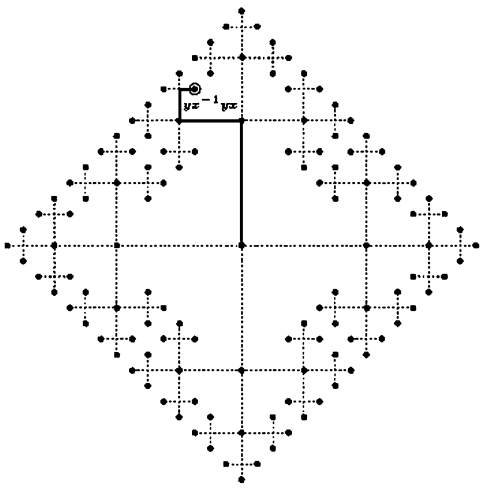
\includegraphics[scale=0.4]{Cayley_graph.png}
\end{figure}
\end{example}

\begin{theorem}[Універсальна властивість вільних груп]
Нехай $G$ --- буде-яка група та $f \colon A \to G$ --- буд-яка функція. Тоді існує єдиний гомоморфізм $\varphi \colon F(A) \to G$, для якого $\varphi \circ j = f$.
\begin{figure}[H]
\centering
\begin{tikzcd}
F(A) \arrow[r,"\varphi"] & G \\
A \arrow[u,"j"] \arrow[ur,"f"] &
\end{tikzcd}
\end{figure}
У цьому випадку відображення $j \colon A \to F(A)$ працює типу як тотожне.
\end{theorem}

\begin{proof}
Оскільки в нас є функція $f \colon A \to G$, то її можна роширити до функції $\tilde{\varphi} \colon W(A) \to G$ так, що на кожній літері $a \mapsto f(a)$ та $a^{-1} \mapsto (f(a))^{-1}$ (\textit{наприклад, $a_1 a_2 \mapsto f(a_1) f(a_2)$}). Зауважимо, що $\tilde{\varphi}(R(w)) = \tilde{\varphi}(w)$, просто тому що виконується $\tilde{\varphi}(r(w)) = \tilde{\varphi}(w)$. Тобто коректно в нас визначене відображення $\varphi \colon F(A) \to G$, яке буде гомоморфізмом, адже $\tilde{\varphi}(ww') = \tilde{\varphi}(w) \tilde{\varphi}(w')$.\\
Цілком ясно, що $\varphi \circ j = f$ в цьому випадку.
\bigskip \\
Єдиність такого відображення цілком ясна.
\end{proof}

\begin{example}
Як по-іншому довести, що $F(\{a\}) \cong \mathbb{Z}$?
\bigskip \\
Розглянемо відображення $j \colon \{a\} \to \mathbb{Z}$, де $a \mapsto 1$, а також будь-яку функцію $f \colon \{a\} \to G$, причому позначимо $f(a) = g$. Тоді визначимо функцію $\varphi \colon \mathbb{Z} \to G$, що задається як $\varphi(1) = g$, а далі можна продовжити до гомоморфізма $\varphi(n) = g^n$. Отже, $\mathbb{Z}$ задовольняє універсальну властивість, ми маємо дві діаграми:
\begin{figure}[H]
\centering
\begin{tikzcd}
F(\{a\}) \arrow[r] & G \\
\{a\} \arrow[u] \arrow[ur,"f"] &
\end{tikzcd}
\qquad
\begin{tikzcd}
\mathbb{Z} \arrow[r,"\varphi"] & G \\
\{a\} \arrow[u,"j"] \arrow[ur,"f"] &
\end{tikzcd}
\end{figure}
Це виконується для будь-яких груп. Зокрема якщо в першу підставити $G = \mathbb{Z}$, а в другу $G = F(\{a\})$, то одержмо, що $F(\{a\}) \cong \mathbb{Z}$.
\end{example}

\subsection{Простота групи $A_n$}
Одразу можемо розглядати випадок $n \geq 3$, просто тому що в інших випадках знакозмінна група буде тривіальною, а тому непростою.

\begin{theorem}
Справедливе наступне:
\begin{itemize}[nosep,wide=0pt]
\item $A_3$ --- проста;
\item $A_4$ --- непроста;
\item $A_n$ --- проста для всіх $n \geq 5$.
\end{itemize}
\end{theorem}

\subsubsection{Простота $A_3$}
(TODO: переписати, оскільки є простіший спосіб: лему перекинути до $A_n$).

\begin{lemma}
\label{A_n_is_generated_by_3_cycles}
Група $A_n$ породжена циклами довжини $3$.
\end{lemma}

\begin{proof}
Оскільки $\sigma \in A_n$, то одержимо в розкладі парну кількість транспозицій:
\[
\sigma = (\tau_1 \circ \tau_2) \circ \dots (\tau_{2k-1} \circ \tau_{2k}).
\]
Нам досить довести, що добуток $(\tau_1 \circ \tau_2)$ породжується циклами довжини $3$. Ці дві транспозиції позначимо
\[
\tau_1 = (ij), \qquad \tau_2 = (kl).
\]
Виникають кілька випадків:
\begin{enumerate}[nosep,wide=0pt,label={\arabic*)}]
\item $\card(\{i,j\} \cap \{k,l\}) = 2$. \\
Фактично кажучи, $\tau_1 = \tau_2$. Звідси випливає, що
\[ 
\tau_1 \circ \tau_2 = (ij) \circ (kl) = (ij)^2 = \varepsilon = (123) \circ (123) \circ (123).
\]
\item $\card(\{i,j\} \cap \{k,l\}) = 1$. \\
Не втрачаючи загальності, нехай $j = l$. Тоді звідси 
\[
\tau_1 \circ \tau_2 = (ij) \circ (kj) = (ijk).
\]
\item $\card(\{i,j\} \cap \{k,l\}) = 0$.\\
Фактично кажучи, ці транспозиції незалежні. Звідси отримаємо 
\[
\tau_1 \circ \tau_2 = (ij) \circ (kl) = (ijk) \circ (jkl). \qedhere
\]
\end{enumerate}
\end{proof}

Тепер готові довести перший пункт теореми. Розглянемо $S_3$, де всього два цикли довжини $3$:
\[
\sigma_1 = (123),\ \sigma_2 = (132).
\]
причому можна зауважити, що насправді 
\[
\sigma_2 = \sigma_1^2.
\]
За вище доведеною лемою та щойно одержаною рівністю маємо
\[
A_3 = \left< \sigma_1, \sigma_2 \right> = \left< \sigma_1 \right>.
\]
Отже, $A_3$ --- циклічна група, причому $|A_3| = 3$. Тоді $A_3$ вона містить лише тривіальні підгрупи, а тому це --- проста група.

\subsubsection{Простота $A_4$}
\begin{lemma}[Спряженість в $S_n$]
Нехай $\tau,\sigma \in S_n$, причому
\[
\sigma = (a_1 \dots a_r) \circ (b_1 \dots b_s) \circ \dots \circ (c_1 \dots c_t).
\]
Тоді спряженість має такий вигляд:
\[
\tau \circ \sigma \circ \tau^{-1} = (\tau(a_1)\dots \tau(a_r)) \circ (\tau(b_1)\dots \tau(b_s)) \circ \dots \circ (\tau(c_1)\dots \tau(c_t)).
\]
\end{lemma}

\begin{proof}
Легко зауважити, що виконуєтсья наступне:
\[
\tau \circ \sigma \circ \tau^{-1} = \tau \circ (a_1 \dots a_r) \circ \tau^{-1} \circ \tau \circ (b_1 \dots b_s) \circ \tau^{-1} \circ \dots \circ \tau \circ (c_1 \dots c_t) \circ \tau^{-1}.
\]
Отже, достатньо довести лему лише для циклів:\\
\[
\tau \circ (a_1 \dots a_r) \circ \tau^{-1} = (\tau(a_1) \dots \tau(a_r)).
\]
Позначимо $\sigma = \tau (a_1 \dots a_r) \tau^{-1}$. Припустимо, що $\tau(a_i) = b_i$. Хочемо довести, що $\sigma = (b_1,\dots,b_r)$.
\begin{align*}
\sigma(b_i) = \tau (a_1 \dots a_r) \tau^{-1} (b_{i}) = \tau (a_1 \dots a_r) (a_i) = \tau (a_{i+1}) = b_{i+1}. \\
\sigma(k) = \tau (a_1 \dots a_r) \tau^{-1}(k) = \tau (a_1 \dots a_r) (m) = \tau (m) = k \text{ при } k \notin \{b_1,\dots,b_r\}.
\end{align*}
Припускаючи, що $\tau(m) = k$, зауважимо, що при цьому $m \notin \{a_1,\dots,a_r\}$.
\end{proof}

\begin{definition}
\textbf{Циклічним типом перестановки $\sigma \in S_n$} називають розбиття числа $n$, що відповідає набору довжин незалежних циклів (\textit{включаючи цикл довжини $1$}), добутком яких є $\sigma$.
\end{definition}

\begin{example}
Наприклад, розглянемо перестановку
\[
\sigma = (14) \circ (23756) \textcolor{red}{\circ (8)}.
\]
Тоді його циклічним типом буде розбиття $(2,5,1)$.
\end{example}

\begin{corollary}
Нехай $\sigma, \sigma' \in S_n$. Тоді
\begin{center}
$\sigma, \sigma'$ --- спряжені $\iff \sigma, \sigma'$ мають однаковий циклічний тип.
\end{center}
\end{corollary}

\begin{proof}
\rightproof \textit{див. попередню лему.}
\bigskip \\
\leftproof Дано: $\sigma,\sigma'$ мають однаковий циклічний тип $(r,s\dots,t)$. Отже, маємо
\begin{align*}
\sigma = (a_1 \dots a_r) \circ (b_1 \dots b_s) \circ \dots \circ (c_1 \dots c_t); \\
\sigma' = (a'_1 \dots a'_r) \circ (b'_1 \dots b'_s) \circ \dots \circ (c'_1 \dots c'_t).
\end{align*}
Визначимо відображення $\tau \colon \{1,\dots,n\} \to \{1,\dots,n\}$ таким чином:
\[ 
\tau(a_i) = a_i',\ \tau(b_j) = b_j',\ \tau(c_k) = c_k'.
\]
Зауважимо, що воно задає бієкцію в силу того, що всі носії кожної перестановки утворюють розбиття $\{1,\dots,n\}$. Таким чином, $\tau \in S_n$. Нарешті,
\begin{align*}
\tau \circ \sigma \circ \tau^{-1} & = (\tau(a_1)\dots \tau(a_r)) \circ (\tau(b_1)\dots \tau(b_s)) \circ \dots \circ (\tau(c_1)\dots \tau(c_t)) \\ 
& = (a'_1 \dots a'_r) \circ (b'_1 \dots b'_s) \circ \dots \circ (c'_1 \dots c'_t) = \sigma'.
\end{align*}
Тим самим довели спряженість $\sigma,\sigma'$.
\end{proof}

Тепер готові довести другий пункт теореми. Розглянемо $S_4$ та всі перестановки вигляду $(2,2)$, яких всього три: 
\[
\sigma_1 = (12)(34),\ \sigma_2 = (13)(24),\ \sigma_3 = (14)(23).
\]
Зауважимо, що всі $\sigma_1,\sigma_2,\sigma_3 \in A_n$, причому кожний з них має порядок $2$. Також зазначимо, що $\sigma_i \sigma_j = \sigma_k$ при різних $i,j,k \in \{1,2,3\}$.\\
Разом із цими результатами, множина 
\[
K = \{\varepsilon,\sigma_1,\sigma_2,\sigma_3\}
\]
утворює підгрупу $A_4$. Більш того, $K \triangleleft A_4$, тому що всі перестановки одного типу --- спряжені. Тим самим довели, що $A_4$ --- непроста група.

\begin{definition}
Отримана підгрупа $K$ називається \textbf{четвертою групою Кляйна}\footnote{Ще інколи зустрічаю позначення $V$ від Vierergruppe.}. Вона складається з 4 елементів, кожний з який оборотний самому себе.
\end{definition}

\subsubsection{Простота $A_n$ при $n \geq 5$}
\begin{lemma}
Всі цикли довжини $3$ спряжені в $A_n$ при $n \geq 5$.
\end{lemma}

\begin{proof}
Нехай $\sigma = (ijk)$. Досить довести, що $\sigma$ спряжена з елементом $(123)$. \\
Для цього зафіксуємо бієкцію $\tau \colon \{1,\dots,n\} \to \{1,\dots,n\}$ таким чином: 
\[
\tau(i) = 1,\quad \tau(j) = 2,\quad \tau(k) = 3.
\]
Звідси одержимо, що
\[
\tau \circ \sigma \circ \tau^{-1} = (\tau(i) \tau(j) \tau(k)) = (123).
\]
Якщо $\tau \in A_n$, то все автоматично доведено.\\
Якщо $\tau \notin A_n$, то розглянемо перестановку $\tilde{\tau} = (45) \circ \tau$. Тепер $\tilde{\tau} \in A_n$, причому 
\[
\tilde{\tau}(i) = \tau(i) = 1,\ \tilde{\tau}(j) = \tau(j) = 2,\ \tilde{\tau}(k) = \tau(k) = 3. \qedhere
\]
\end{proof}

\begin{remark}
Що відбувається з іншими знакозмінними групами $A_n$, коли $n \in \{3,4\}$.
\bigskip \\
В групі $A_3$ зауважимо, що $(123)$ не спряжений з $(132)$. Який б $\tau \in A_3$ не взяв, $(123) \neq \tau (132) \tau^{-1}$.\\
В групі $A_4$ Кількість класів спряженості ділить $|A_n| = 12$, кількість $3$-циклів тут всього $8$. Значить, всі вони не лежать в одному класу спряженості.
\end{remark}

\begin{lemma}
Нехай $\sigma \in A_n$ при $n \geq 5$ --- нетривіальна перестановка, що не є циклом довжини $3$. Тоді існує перестановка $\tau \in A_n$, для якої $\tau \sigma \tau^{-1} \sigma^{-1}$ (\textit{тобто комутатор $\tau,\sigma$}) також нетривіальна та має більше нерухомих точок, аніж $\sigma$.
\end{lemma}

\begin{proof}
Розіб'ємо доведення на два можливих випадки.

\begin{enumerate}[wide=0pt,label={\Roman*.}]
\item \textit{$\sigma$ розписується як добуток неперетинних транспозицій}.\\
Оскільки $\sigma \in A_n$ та $\sigma \neq \varepsilon$, то в добутку хоча б дві неперетинних транспозиції. Запишемо це як
\[ 
\sigma = (ij)(kl) \rho,
\]
де перестановка $\rho$ --- це добуток решти транспозицій, що має уже нерухомі точки $i,j,k,l$ (\textit{можлива відсутність $\rho$, оскільки $\sigma$ може мати рівно дві транспозиції}). Покладемо 
\[
\tau = (klt) \in A_n,
\]
де точка $t \in \{1,2,\dots,n\} \setminus \{i,j,k,l\}$, яка існує, оскільки $n \geq 5$.\\
Тепер розглянемо перестановку $\tau \sigma \tau^{-1} \sigma^{-1}$. Проаналізуємо на наявність нерухомих точок.\\
Точки $i,j$ не будуть нерухомими для $\sigma$, але будуть нерухомими для $\tau \sigma \tau^{-1} \sigma^{-1}$, оскільки
\begin{align*}
\tau \sigma \tau^{-1} \sigma^{-1} (i) = \tau \sigma \tau^{-1}(j) = \tau \sigma(j) = \tau(1) = i; \\
\tau \sigma \tau^{-1} \sigma^{-1} (j) = \tau \sigma \tau^{-1}(i) = \tau \sigma (i) = \tau (2) = j.
\end{align*}
Точки $k,l$ уже не будуть нерухомими як для $\sigma$, так і для $\tau \sigma \tau^{-1} \sigma^{-1}$, внаслідок чого $\tau \sigma \tau^{-1} \sigma^{-1} \neq \varepsilon$. Наприклад,
\[
\tau \sigma \tau^{-1} \sigma^{-1} (k) = \tau \sigma \tau^{-1} (l) = \tau \sigma(k) = \tau(l) = t.
\]
(\textit{при $n = 5$ уже закінчили, по суті}). Оберемо нерухому точку $f \in \{1,\dots,n\} \setminus \{i,j,k,l,t\}$ для $\sigma$, тоді $f$ буде нерухомою точкою для $\tau \sigma \tau^{-1} \sigma^{-1}$, оскільки 
\[
\tau \sigma \tau^{-1} \sigma^{-1} (f) = \tau \sigma \tau^{-1} (f) = \tau \sigma (f) = \tau (f) = f.
\]
Отже, $\tau \sigma \tau^{-1} \sigma^{-1}$ має більше нерухомих точок, аніж $\sigma$.

\item \textit{$\sigma$ не розписується як добуток неперетинних транспозицій}.\\
Тоді існує цикл довжини хоча б три. Запишемо як 
\[
\sigma = (ijk \dots) \rho,
\]
де $\rho$ діє має хоча б нерухомі точки $i,j,k$. За умовою леми $\sigma \neq (ijk)$, тобто не є 3-циклом. Щонайменше п'ять точок $\sigma$ зобов'язані бути рухомими.\\
Якби були лише три рухомих точок, то одержали б $\sigma = (ijk)$, що неможливо за умовою.\\
Якби були лише чотири рухомих точок, то одержали б $\sigma = (ijkr)$, але тоді $\sigma \notin A_n$, що неможливо.\\
Тож $\sigma$ зобов'язана мати принаймні такий вигляд:
\[
\sigma = (ijklt \dots) \tilde{\rho}.
\]
Знову оберемо перестановку
\[
\tau = (klt) \in A_n.
\]
По-перше зауважимо, що $\tau \sigma \tau^{-1} \sigma^{-1} \neq \varepsilon$, тому що
\[
\tau \sigma \tau^{-1} \sigma^{-1}(k) = \tau \sigma \tau^{-1} (j) = \tau \sigma (j) = \tau (k) = l.
\]
Тепер проаналізуємо на наявність нерухомих точок.\\
Гарантовано точки $i,j,k,l,t$ не будуть нерухомими для $\sigma$. При цьому точка $j$ буде нерухомою для $\tau \sigma \tau^{-1} \sigma^{-1}$ (\textit{при $n = 5$ уже закінчили, по суті}).\\
Нехай $f \notin \{i,j,k,l,t\}$ --- нерухома для $\sigma$, тоді аналогічними міркуваннями $f$ буде нерухомою для $\tau \sigma \tau^{-1} \sigma^{-1}$. Отже, $\tau \sigma \tau^{-1} \sigma^{-1}$ містить більше нерухомих точок, аніж $\sigma$. \qedhere
\end{enumerate}
\end{proof}

Тепер готові довести третій пункт теореми. Нехай $N \triangleleft A_n$, яка нетривіальна. Оберемо нетривіальну перестановку $\sigma \in N$ з найбільшим числом нерухомих точок. Тоді $\sigma$ буде $3$-циклом.\\
!Припустимо, що $\sigma$ не є $3$-циклом. За щойно доведеною лемою існує перестановка $\tau \in A_n$, для яких $\tau \sigma \tau^{-1} \sigma^{-1} \neq \varepsilon$ та місить більше нерухомих точок, аніж $\sigma$. При цьому оскільки $\sigma^{-1} \in N$ та $\tau \sigma \tau^{-1} \in N$ в силу нормованості, то $\tau \sigma \tau^{-1} \sigma^{-1} \in N$ --- суперечність за кількістю нерухомих точок!\\
Отже, $\sigma \in N$ буде $3$-циклом. Відомо, що в групі $A_n$ при $n \geq 5$ всі $3$-цикли спряжені, внаслідок чого $N = A_n$.

\subsubsection*{Про групу $A_\infty$}
Взагалі-то кажучи, можна визначити групу $S_\infty \eqbydef S_{\mathbb{N}}$. Іншими словами, просто колекція бієкцій $\mathbb{N} \to \mathbb{N}$. Далі можна визначити $S_{\infty}^{\text{finite}}$ --- підгрупа $S_\infty$, яка містить бієкції, зі скінченним числом рухомих точок. Нарешті, можна визначити підгрупу $A_\infty$, яка породжена всіма $3$-циклами. Тоді цілком зрозуміло, що $A_\infty \triangleleft S_{\infty}^{\text{finite}}$.
\bigskip \\
Всередині групи справедлива аналогічна лема, що якщо $\sigma \in A_\infty$, яка нетривіальна та не $3$-цикл, то існує перестановка $\tau \in A_\infty$ така, що $\tau \sigma \tau^{-1} \sigma^{-1}$ також нетривіальна та міститиме менше рухомих точок за $\sigma$. А далі схожими міркуваннями, як було вище, можна довести наступне:

\begin{theorem}
$A_\infty$ --- проста група (\textit{приклад нескінченної простої групи}).
\end{theorem}

\subsection{Нормальні замикання}
\begin{definition}
Задано $\left< G, *\right>$ -- група та $M \subset G$.\\
\textbf{Нормальним замиканням множини $M$ в групі $G$}, називають таку множину:
\begin{align*}
\ncl_G(M) = \bigcap_{\substack{H \triangleleft G \\ H \supset M}} H
\end{align*}
Альтернативне позначення: $\left< M \right>_n$.\\
Тобто $\ncl_G(M)$ -- найменша нормальна підгрупа $G$ (легітимним чином є підгрупою), що містить $M$.
\end{definition}

\begin{theorem}
Задано $\left<G,*\right>$ -- група та $M \subset G$.\\
Тоді $\ncl_G(M) = \left< M^G \right>$, у цьому випадку $M^G = \{m^x \mid m \in M,x \in G\}$.
\end{theorem}

\begin{proof}
$\left<M^G \right> \subset \ncl_G(M)$\\
Дійсно, нехай $m^x \in \left<M^G\right>$. Оскільки $m \in M$, то звідси $m \in \ncl_G(M)$. Але водночас $x \in G$ та $\ncl_G(M) \triangleleft G$, звідси $m^x = x^{-1}*m*x \in \ncl_G(M)$.\\
Якщо взяти елемент $u \in \left< M^G \right>$, то він розписується на добуток елементі $m^x \in \ncl_G(M)$. Таким чином, $u \in \ncl_G(M)$.
\bigskip \\
$\ncl_G(M) \subset \left< M^G \right>$.\\
Достатньо довести, що $\left< M^G \right> \triangleleft G$ та $M^G \supset M$.\\
Те, що $M^G \subset M$, це зрозуміло просто через те, що $e \in G$.\\
Для першого зауважимо, що для $x \in G$ виконується така рівність:\\
$\left(\left< M^G \right>\right)^x = \left< (M^{G})^x \right> = \left< M^{G*x} \right> = \left< M^G \right>$.\\
Ця рівність свідчить про те, що $M^G \triangleleft G$.\\
Тоді $\ncl_G(M) \subset \left<M^G\right>$, бо друга множина в цьому перетині.
\end{proof}

\begin{theorem}[Про побудову комутанта підгрупи, що породжена множиною]
Задано $G = \left< M \right>$. Тоді $G' = \ncl_G(M')$, тут позначили \\
$M' = \{ [m_1,m_2] \mid m_1,m_2 \in M\}$.
\end{theorem}

\begin{proof}
$\ncl_G(M') \subset G'$.\\
За попередньою теоремою, $\ncl_G(M')$ породжується елементами $[m_1,m_2]^x, x \in G$. Зрозуміло, що $[m_1,m_2] \in G'$, але $G' \triangleleft G$. Отже, $[m_1,m_2]^x \in G'$.\\
Кожний елемнт $u \in \ncl_G(M')$ записується як добуток з елементів $[m_1,m_2]^x \in G'$. Значить, $u \in G'$.
\bigskip \\
$G' \subset \ncl_G(M')$.\\
Ми вже знаємо, що $G' \subset \ncl_G(M') \subset G \iff \ncl_G(M') \triangleleft G$ та $G/_{\ncl_G(M')}$ -- абелева (основа теорема про комутант). Перша умова вже виконана, залишилася друга.\\
Розглянемо проєкцію $\pi \colon G \to G/_{\ncl_G(M')}$. Зауважимо, що\\
$[m_1,m_2]*\ncl_G(M') = [m_1*\ncl_G(M'),m_2*\ncl_G(M')]$. Оскільки $[m_1,m_2] \in \ncl_G(M')$, то звідси $[m_1*\ncl_G(M'),m_2*\ncl_G(M')] = e*\ncl_G(M')$. Отже, два суміжні класи комутують.\\
За еквівалентністю, $G' \subset \ncl_G(M)$.
\end{proof}

\subsection{Напівпрямий добуток}
\begin{definition}
Нехай $\left<G,*\right>,\ \left<H, \star\right>$ --- групи, а також гомоморфізм $\varphi \colon H \to \Aut(G)$.\\
\textbf{Напівпрямим добуток} називають групу, що складається з множини $G \times H$ та операції $\cdot$:
\begin{align*}
(g_1,h_1) \cdot (g_2,h_2) = (g_1*\varphi(h_1)(g_2), h_1 \star h_2).
\end{align*}
(\textit{іншими словами, тепер ми не просто втупу перемножуємо $g_1*g_2$, а перемножуємо так, що цей елемент $g_2$ якимось чином ''перекручується''}).\\
\textit{Позначення}: $\left<G \rtimes_\varphi H,\ \cdot\right>$.
\end{definition}

\begin{remark}
Якщо взяти гомоморфізм $\varphi = \id$, то зауважимо, що тоді
\begin{align*}
(g_1,h_1) \cdot (g_2,h_2) = (g_1*\id(h_1)(g_2), h_1 \star h_2) = (g_1*g_2, h_1 \star h_2).
\end{align*}
Тобто ми одержали класичний прямий добуток груп, тобто
\[
G \rtimes_{\id} H = G \times H
\]
(\textit{ми тепер $g_2$ ніяк не ''перекручуємо''}).
\end{remark}

\begin{proposition}
Структура $\left<G \rtimes_\varphi H,\ \cdot\right>$ дійсно задає групу.
\end{proposition}

\begin{proof}
\begin{enumerate}[wide=0pt,topsep=0pt,label={\Roman*.}]
\item \textit{Асоціативність}.\\
Отже, нехай $(g_1,h_1), (g_2,h_2), (g_3,h_3) \in G \rtimes H$, тоді з одного боку,
\[
(g_1,h_1) \cdot ((g_2,h_2) \cdot (g_3,h_3)) = (g_1,h_1) \cdot (g_2 * \varphi(h_2)g_3, h_2 \star h_3) = (g_1*\varphi(h_1)(g_2*\varphi(h_2)g_3), h_1 \star (h_2 \star h_3)).
\]
Із іншого боку, маємо
\[
((g_1,h_1) \cdot (g_2,h_2)) \cdot (g_3,h_3) = (g_1*\varphi(h_1)g_2, h_1 \star h_2) \cdot (g_3,h_3) = (g_1*\varphi(h_1)g_2*\varphi(h_1 \star h_2)g_3, (h_1 \star h_2) \star h_3).
\]
Другі координати рівні, оскільки в групі $H$ в нас виконується асоціативність $\star$. Перші координати також рівні, оскільки
\[
g_1 * \varphi(h_1)(g_2* \varphi(h_2)g_3) = g_1 * \varphi(h_1)(g_2) * (\varphi(h_1) \circ \varphi(h_2))(g_3) = g_1 * \varphi(h_1)(g_2) * \varphi(h_1 \star h_2)g_3. 
\]

\item \textit{Існування нейтрального елементу}.\\
Нейтральним елементом буде $(e,e)$, просто тому що
\[
(g,h) \cdot (e,e) = (g*\varphi(h)e, h \star e) = (g*e, h \star e) = (e,e).
\]
\[
(e,e) \cdot (g,h) = (e*\varphi(e)g, e \star h) = (e*g, e \star h) = (e,e).
\]
\item \textit{Існування оборотного елементу}.\\
Нехай $(g,h) \in G \rtimes H$. Хочемо знайти такий елемент $(a,b) \in G \rtimes H$, щоб
\[
(g,h) \cdot (a,b) = (g*\varphi(h)a, h \star b) = (e,e).
\]
Із другої координатної рівності ясно, що тоді $b = h^{-1}$. Із першою координатою ситуація цікавіша, там тоді $\varphi(h)(a) = g^{-1}$. Однак оскільки $\varphi(h)$ є ізоморфізмом, то можемо подіяти з двох сторін на $(\varphi(h))^{-1} = \varphi(h^{-1})$. Внаслідок чого $a = \varphi(h^{-1})(g^{-1})$.\\
Отже, оборотним елементом до $(g,h)$ буде елемент $(\varphi(h^{-1})(g^{-1}), h^{-1})$. \qedhere
\end{enumerate}
\end{proof}

\begin{example}
Зокрема $D_n \cong \mathbb{Z}_n \rtimes \mathbb{Z}_2$.
\bigskip \\
Для цього визначимо відображення $\varphi \colon \mathbb{Z}_2 \to \Aut(\mathbb{Z}_n)$ ось так:
\begin{align*}
\varphi(\overline{n})(\overline{m}) = \overline{n-m}.
\end{align*}
Утворили такий напівпрямий добуток $\mathbb{Z}_n \rtimes_\varphi \mathbb{Z}_2$. Гомоморфізм $f \colon \mathbb{Z}_n \rtimes \mathbb{Z}_2 \to D_n$ можна визначити ось так:
\begin{align*}
f((\overline{m},\overline{k})) = r^m s^k.
\end{align*}
Це буде справді гомоморфізмом, просто тому що
\begin{align*}
f((\overline{m}+\overline{n},\overline{k}+\overline{l})) = f(\overline{m} + \varphi(\overline{n})\overline{k}, \overline{n} + \overline{l}) = f(\overline{m+n-k}, \overline{n+l}) = r^{m+n-k} s^{n+l} = r^{m-k} s^{n+l} \\
r^m s^n \cdot r^k s^l = f(\overline{m},\overline{n}) \cdot f(\overline{k},\overline{l}).
\end{align*}
Оскільки $r^n = e$ та $s^2 = e$, то відображення $f$ задає ізоморфізм.
\end{example}

\begin{example}
Зокрема $S_n \cong A_n \rtimes \mathbb{Z}_2$.
\bigskip \\
Дійсно, $A_n \triangleleft S_n$, при цьому $S_n \cap A_n = \{\varepsilon\}$, а також $S_n = A_n \left<\tau\right>$, де $\tau \in S_n$ --- деяка транспозиція (\textit{TODO: додати про внутрішній прямий добуток}).
\end{example}

\begin{example}
Також можна взяти $S_4 \cong V_4 \rtimes S_3$.
\end{example}

\begin{example}
Зокрема $A(n,F) \cong F^n \rtimes GL_n(F)$.
\end{example}

\begin{proposition}
Нехай $G,H$ --- групи. Тоді нижчі відображення задають гомоморфізм:
\begin{align*}
\rho \colon G \to G \rtimes H, \qquad \rho(g) = (g,e_H); \\
\pi \colon G \rtimes H \to H, \qquad \pi(g,h) = h; \\
\sigma \colon H \to G \rtimes H, \qquad \sigma(h) = (e_G,h).
\end{align*}
Зокрема можна зауважити, що $G \cong G \times \{e_H\}$, а також $H \cong \{e_G\} \times H$.\\
\textit{Вправа: довести}.
\end{proposition}

\begin{remark}
Говорячи категоріальною мовою, ми одержили коротку точну послідовність, яка допускає переріз\footnote{Якщо в нас є гомоморфізм груп $p \colon G \to H$, \textbf{перерізом $p$} називають гомоморфізм $s \colon H \to G$, що задовольняє умову $p \circ s = \id$. Зауважимо, що при існуванні перерізу $p$ обов'язково має бути сюр'єктивним, а тому $s(H)$ можна сприймати як підгрупу $G$. Ну й ще скажу, що не всякий гомоморфізм може мати переріз, наприклад $\mathbb{Z} \to \mathbb{Z}_n$, де $k \mapsto k \mod n$ при $n \geq 2$.}:
\begin{figure}[H]
\centering
\begin{tikzcd}
G \arrow[r,hook,"\rho"] & G \rtimes H \arrow[r,two heads,"\pi"] & H \arrow[l,bend left = 30, "\sigma"]
\end{tikzcd}
\end{figure}
\end{remark}
\newpage

\section{Класифікація абелевих груп}
Надалі всюди $\left< G, *\right>$ --- абелева група. Для зручності нейтральний елемент позначатимемо за $0$, обернений елемент до $a$ позначимо за $-a$, а операцію позначатимемо $+$. Крім того, замість $g^m$ позначатимемо $m \cdot g$.
\bigskip \\
Крім того, якщо маємо дві абелеві групи $G_1,G_2$, то замість прямого добутку $G_1 \times G_2$ будемо позначати $G_1 \oplus G_2$ та називати прямою сумою груп.

\subsection{Скрути}
\begin{definition}
Маємо групу $\left< G, +\right>$.\\
Групу $G$ називають \textbf{групою без скруту}, якщо
\begin{align*}
\forall g \in G \setminus \{0\}: \ord(g) = \infty.
\end{align*}
Групу $G$ називають \textbf{групою зі скрутом}, якщо
\begin{align*}
\forall g \in G: \ord(g) < \infty.
\end{align*}
Інакше така група $G$ буде \textbf{мішаною групою}.
\end{definition}

% Жодні групи не ізоморфні між собою

\begin{example}
Зокрема маємо такі приклади:
\begin{itemize}[nosep,wide=0pt]
\item $\mathbb{Q}$ --- група без скруту;
\item $\mathbb{Q}/_{\mathbb{Z}}$ --- група зі скрутом;
\item $\mathbb{C}$ --- мішана група.
\end{itemize}
\end{example}

\begin{proposition}
Нехай $G$ --- група, позначимо $T(G)$ ось так:
\begin{align*}
T(G) = \{ g \in G \mid \ord(g) < \infty\}.
\end{align*}
Тоді $T(G) \leq G$, а також $G/_{T(G)}$ буде групою без скрутів.
\end{proposition}

\begin{definition}
Підгрупа $T(G)$ називається \textbf{підгрупою скрутів}.
\end{definition}

\begin{proof}
\begin{enumerate}[topsep=0pt,wide=0pt,label={\Roman*.}]
\item $T(G) \leq G$.\\
Нехай $a,b \in T(G)$, тобто маємо скінченний порядок $\ord(a) = m,\ \ord(b) = n$. Звідси
\[
mn \cdot (a-b) = mn \cdot a - mn \cdot b = 0 - 0 = 0,
\]
звідси випливає, що $\ord(a-b) < \infty$.

\item \textit{$G/_{T(G)}$ --- група без скруту}.\\
Нехай $\ord(g+T(G)) = n$, тобто маємо
\[
n (g+T(G)) = ng + T(G) = T(G).
\]
Звідси одержимо, що $ng \in T(G)$, тобто $\ord(ng)$ --- скінченний, позначимо $\ord(ng) = m$. Звідси $m \cdot (ng) = (mn) \cdot g = 0$, а тому $g \in T(G)$. Одержали, що 
\[
g+T(G) = T(G).
\]
Отже, лише нейтральний елемент $T(G)$ може мати скінченний порядок в групі $G/_{T(G)}$. \qedhere
\end{enumerate}
\end{proof}

\begin{theorem}
Нехай $G$ --- будь-яка група зі скрутом та $p$ --- просте число. Позначимо
\begin{align*}
G_p = \{g \in G \mid \ord g = p^k \text{ для деякого $k$}\}.
\end{align*}
Тоді, позначивши $P$ за множину всіх простих чисел, одержимо наступне:
\begin{align*}
G = \sum_{p \in P} G_p
\end{align*}
\end{theorem}

\begin{proof}
Нехай $g \in G$, його порядок скінченний, запишемо за основною теоремою арифметики як
\[
\ord(g) = p_1^{r_1} \dots p_n^{r_n}.
\]
Позначимо $q = p_1^{r_1} \dots p_{n-1}^{r_{n-1}}$, тоді зауважимо, що $\gcd(q, p_n^{r_n}) = 1$. За рівністю Безу
\[
aq + bp_n^{r_n} = 1
\]
для деяких $a,b \in \mathbb{Z}$, внаслідок чого
\[
g = aq g + b p_n^{r_n} g.
\]
Зауважимо, що $\ord(aqg) = p_n^{r_n}$, тому звідси $aqg \in G_{p_n}$. Крім того, $\ord(bp_n^{r_n} g) = q$, однак оскільки $q < \ord(g)$, можна індуктивно припустити, що $bp_n^{r_n} g$ є сумою елементів, що належать $Gp_{n-1}, \dots, G_{p_1}$. Тому будь-який елемент $G$ записується як сума елементів, що належать $G_p$ (TODO: для чого цей параграф?).
\bigskip \\
Тепер доведемо, що коли $g_1 + \dots + g_n = 0$, то $g_1 = \dots = g_n = 0$ за МІ.
\end{proof}

\begin{definition}
Підгрупи $G_p$ називаються \textbf{$p$-компонентами} групи $G$.
\end{definition}

\subsection{Вільні абелеві групи}
Ситуація трохи відрізняється. Здавалось би, можемо попросити, щоб літери з $A \cup A'$ комутували між собою --- і тоді буде абелева група $\left<F(A), \cdot \right>$. Проте ''вільна'' означає група, в яких нема взаємних зв'язків з літерами, тому так не пройде.
\bigskip \\
Якщо попросити, щоб $\forall x,y \in A \cup A'$ ми мали б $xy = yx$, то слова
\[
xyz,\ yxz,\ zxy,\ zyx,\ xzy,\ yzx
\]
мають бути одними й тими самими словами. В групі $F(A)$ це зовсім різні скорочені слова. Однак можна створити факторгрупу
\[
F^{\text{ab}}(A) = F(A)/_{[F(A),F(A)]},
\]
яка є абеленізацією.

\begin{corollary}
Утворена група $\left<F^{\text{ab}}, \cdot \right>$ є абелевою групою та називається \textbf{вільною абелевою групою}.
\end{corollary}

\begin{theorem}[Універсальна властивість вільних абелевих груп]
Нехай $G$ --- буде-яка абелева група та $f \colon A \to G$ --- буд-яка функція. Тоді існує єдиний гомоморфізм $\varphi \colon F^{\text{ab}}(A) \to G$, для якого $\varphi \circ j = f$.
\begin{figure}[H]
\centering
\begin{tikzcd}
F^{\text{ab}}(A) \arrow[r,"\varphi"] & G \\
A \arrow[u,"j"] \arrow[ur,"f"] &
\end{tikzcd}
\end{figure}
У цьому випадку відображення $j \colon A \to F^{(ab)}(A)$ працює як $a \mapsto a \cdot [F(A),F(A)]$.
\end{theorem}

\begin{proof}
Уже відомо за універсальною властивістю стандартних вільних груп, що існує єдиний гомоморфізм $\bar{\varphi} \colon F(A) \to G$, для якого комутує діаграма:
\begin{figure}[H]
\centering
\begin{tikzcd}
F(A) \arrow[r,"\varphi"] & G \\
A \arrow[u,"j"] \arrow[ur,"f"] &
\end{tikzcd}
\end{figure}
Побудуємо відображення $\varphi \colon F^{\text{ab}}(A) \to G$ ось таким чином:
\[
\varphi(w \cdot [F(A),F(A)]) = \bar{\varphi}(w).
\]
Воно коректно визначене. Якщо $w \cdot [F(A),F(A)] = v \cdot [F(A),F(A)]$, тобто $wv^{-1} \in [F(A),F(A)]$, то буде ось таке:
\[
w = [x_1,y_1] [x_2,y_2] \dots [x_n,y_n] v.
\]
Тоді маємо наступне (\textit{і саме тут абелевість групи $G$ нам дуже знадобиться}):
\[
\bar{\varphi}(w) = f(x_1) f(y_1) (f(x_1))^{-1} (f(y_1))^{-1} \dots f(x_n) f(y_n) (f(x_n))^{-1} (f(y_n))^{-1} \bar{\varphi}(v) = \bar{\varphi}(v).
\]
Цілком зрозуміло, що $\varphi$ --- також гомоморфізм груп та задовольняє умову $\varphi \circ j = f$. Єдиність зрозуміла.
\end{proof}

\begin{proposition}
$\mathbb{Z}^{\oplus n}$ задовольняє універсальну властивість вільних абелевих груп.
\end{proposition}

\begin{proof}
По-перше, зауважимо, що елемент $(m_1,\dots,m_n) \in \mathbb{Z}^{\oplus n}$ можна записати ось так:
\begin{align*}
(m_1,\dots,m_n) & = (m_1,0,\dots,0) + (0,m_2,\dots,0) + \dots + (0,0,\dots,m_n) \\
& = m_1 (1,0,\dots,0) + m_2 (0,1,\dots,0) + \dots + m_n (0,0,\dots,1).
\end{align*}
Оберемо множину $A = \{a_1,\dots,a_n\}$, побудуємо $j \colon A \to \mathbb{Z}^{\oplus n}$ ось так: 
\[
j(a_i) = (0,\dots,\underbrace{1}_{i\text{-тий}},\dots,0).
\]
Тоді елемент вище запишеться більш компактно:
\[
(m_1,\dots,m_n) = m_1 j(a_1) + \dots + m_n j(a_n).
\]
Тому якщо є функція $f \colon A \to G$ до будь-якої абелевої групи $G$, то можна побудувати гомоморфізм $\varphi \colon \mathbb{Z}^{\oplus n} \to G$ так:
\[
\varphi(m_1,\dots,m_n) = m_1 f(a_1) + \dots + m_n f(a_n).
\]
Уже видно, що $\varphi \circ j = f$. Крім того, $\varphi$ --- гомоморфізм груп завдяки абелевості $G$.
\end{proof}

\begin{corollary}
Якщо $\# A = n$, то будь-яка вільна абелева група записується ось так:
\begin{align*}
F^{\text{ab}}(A) \cong \underbrace{\mathbb{Z} \oplus \dots \oplus \mathbb{Z}}_{\text{$n$ разів}}.
\end{align*}
Якщо позначити елементи $e_i = (0,\dots,\underbrace{1}_{\text{$i$-тий}},\dots,0)$, то маємо $F^{\text{ab}}(A) \cong \left<e_1,\dots,e_n\right>$, тобто вільна абелева група є скінченно породженою. Нарешті, вільна абелева група не містить скруту.
\end{corollary}


\subsection{Незалежність}
\begin{definition}
Нехай $G$ --- група. Підмножина $X \subset G$ називається \textbf{незалежною}, якщо для будь-яких різних $x_1,\dots,x_r \in X$ та $n_1,\dots,n_r \in \mathbb{Z}$ маємо
\begin{align*}
n_1 x_1 + \dots + n_r x_r = 0 \implies n_1 x_1 = \dots = n_r x_r = 0.
\end{align*}
\end{definition}

\begin{remark}
Якщо $G$ --- група без скруту, то маємо звичне означення:
\begin{align*}
n_1 x_1 + \dots + n_r x_r = 0 \implies n_1 = \dots = n_r = 0.
\end{align*}
В цьому випадку можна це називати лінійно незалежно підмножиною (\textit{як в лінійній алгебрі}).
\end{remark}

\begin{definition}
Елемент $x \in G$ називається \textbf{залежним} в $X$, якщо при деяких $x_1,\dots,x_r \in X$ та деякому $n \in \mathbb{Z}$ маємо
\begin{align*}
nx + n_1 x_1 + \dots + n_r x_r =0,
\end{align*}
причому ось цей $nx \neq 0$.\\
Підмножина $Y \subset G$ називається \textbf{залежною} в $X$, якщо
\begin{center}
будь-який елемент $y \in Y$ буде залежним в $X$.
\end{center}
\end{definition}

\begin{remark}
Нехай $G$ --- група без скруту. Якщо $X$ залежний в $Y$ та $Y$ залежний в $Z$, то тоді $X$ залежний в $Z$. 
\end{remark}

\begin{theorem}[Лема Штайніца про заміну]
Нехай $G$ --- група без скруту та $A = \{a_1,\dots,a_m\} \subset G$ незалежна. Нехай $B = \{b_1,\dots,b_n\} \subset G$, причому $A$ залежна від $B$. Тоді $n \geq m$, а також $B$ залежна від $A \cup C$, причому $C \subset B$ та $\# C = n-m$. 
\end{theorem}

\begin{proof}
Доведення будемо проводити за МІ по $m$.
\begin{enumerate}[wide=0pt,label={\Roman*.}]
\item \textit{База індукції}. При $m = 1$ зрозуміло, що $n \geq 1$. Крім того, оскільки $\{a_1\} = A$ залежить від $B$, то
\[
z a_1 + z_1 b_1 + \dots + z_n b_n = 0
\]
при $z \neq 0$ та деяких $z_1,\dots,z_n \in \mathbb{Z}$. Отже, при деякому $1 \leq i \leq n$ маємо $z_i \neq 0$, внаслідок чого $B$ залежить від $A \cup (B \setminus \{b_i\})$.

\item \textit{Припущення індукції}. При $m = r$ лема Штайніца про заміну виконується.

\item \textit{Крок індукції}. Нехай $m = r+1$. Маємо, що $\{a_1,\dots,a_r\}$ залежить від $B$, то за МІ $B$ залежить від $\{a_1,\dots,a_r\} \cup D$, причому $D \subset B$ та $\# D = n-r$ (\textit{за МІ відомо, що $n \geq r$}). Однак $\{a_{r+1}\}$ залежить від $B$ та $B$ залежить від $\{a_1,\dots,a_r\} \cup D$. Звідси випливає, що $\{a_{r+1}\}$ залежить від $\{a_1,\dots,a_r\} \cup D$. Тобто
\[
ya_{r+1} = y_1 a_1 + \dots + y_r a_r + z_1 d_1 + \dots + z_s d_s
\]
при деяких $y_1,\dots,y_r,z_1,\dots,z_s \in \mathbb{Z}$ та $d_1,\dots,d_s \in D$, причому $y \neq 0$. Гарантовано деякий $z_i \neq 0$ (\textit{інакше $A = \{a_1,\dots,a_{r+1}\}$ перестане бути незалежною множиною}). Крім того, $n > r$ (\textit{інакше $\{a_{r+1}\}$ буде залежати від $\{a_1,\dots,a_r\}$, що знову порушить означення незалежності $A$}), внаслідок чого $n \geq r+1 = m$.\\
Покладемо $C = D \setminus \{d_i\}$. Тоді $\{a_1,\dots,a_r\} \cup D$ залежить від $\{a_1,\dots,a_{r+1}\} \cup C$. Значить, $B$ залежить від $\{a_1,\dots,a_{r+1}\} \cup C$. Нарешті, $C \subset B$ та $\# C = \# D - 1$, тобто $\# C = (n-r)-1 = n-(r+1) = n-m$.
\end{enumerate}
МІ доведено.
\end{proof}

\begin{definition}
Нехай $G$ --- група. Підмножина $S \subset G$ називається \textbf{максимально незалежною}, якщо
\begin{center}
$S$ --- незалежна підмножина; \\
для будь-якого $g \in G \setminus S$ множина $S \cup \{g\}$ буде залежною. 
\end{center}
\end{definition}

\begin{theorem}
Нехай $G$ --- абелева група. Тоді існує максимально незалежна множина.
\end{theorem}

\begin{proof}
Розглянемо ось такий клас:
\begin{align*}
\mathcal{P} = \{X \subset G \mid X \text{ --- незалежна}\}.
\end{align*}
Оберемо довільний ланцюг $\mathcal{C} = \{X_i \mid i \in I\}$ елементів з $\mathcal{P}$. Доведемо, що $\displaystyle\bigcup_{i \in I} X_i = U \in \mathcal{P}$.\\
Цілком ясно, що $U \subset G$. Далі припустимо, що $U$ --- залежна множина, тобто
\[
r_1 u_1 + \dots + r_n u_n = 0
\]
при деяких $u_1,\dots,u_n \in I$ та $r_1,\dots,r_n \in \mathbb{Z}$, де хоча б один $r_i u_i \neq 0$. Оскільки $U = \displaystyle\bigcup_{i \in I} X_i$, то звідси $u_1 \in X_{1'}.\ u_2 \in X_{2'}$, причому або $X_{1'} \subset X_{2'}$, або $X_{2'} \subset X_{1'}$. Коротше, $u_1,u_2$ належать одночасно деякій множині з $\mathcal{C}$. Продовжуючи далі цю махінацію, одержимо, що $u_1,\dots,u_n \in X_i$ при деякому $X_i \in \mathcal{C}$. Проте $X_i$ сама є незалежною множиною --- суперечить нашому припущенню.\\
Далі за лемою Цорна знайдемо максимально можливу множину з $S \in \mathcal{P}$, яка й буде максимально незалежною за означенням.
\end{proof}

\subsection{Ранг групи}
\begin{remark}
Нехай $G$ --- група без скруту та $S,T$ --- дві максимально незалежні підмножини, причому $\# S, \# T < \infty$. Користуючись двічі лемою Штайніца про заміну одержимо $\# T \geq \# S$ та $\# S \geq \# T$. Іншими словами, $\# S = \# T$.
\end{remark}

\begin{definition}
Для групи $G$ без скруту визначимо \textbf{ранг групи} як потужність максимально лінійно незалежної підмножини.\\
Позначення: $\rank G$ (\textit{якщо не існує скінченного максимально лінійно незалежної підмножини, то покладемо $\rank G = \infty$}).
\end{definition}

\begin{remark}
$G \cong H \implies \rank G = \rank H$.
\end{remark}

\begin{example}
Однак навпаки ні, оскільки можна взяти неізоморфні групи $\mathbb{Z}, \mathbb{Q}$, які не мають скрутів та містять обидва ранг $1$.
\end{example}

\begin{remark}
Нехай $F(X)$ --- вільна абелева група (\textit{вона автоматично без скруту}), причому $\# X < \infty$. Тоді $X$ --- макисмально незалежна.
\end{remark}

\begin{corollary}
Якщо $F$ --- вільна абелева група, породжена множинами $X,Y$, то тоді $\# X = \# Y$.
\end{corollary}

\subsection{Основна теорема абелевих груп}
\begin{lemma}
Нехай $G = \left<a_1\right> \oplus \dots \oplus \left<a_n\right>$, де кожна циклічна група нескінченна. Нехай
\[
b = a_1 + r_2 a_2 + \dots + r_n a_n
\]
при деяких $r_2,\dots,r_n \in \mathbb{Z}$. Тоді $G = \left<b_1\right> \oplus \left<a_2\right> \oplus \dots \oplus \left<a_n\right>$.
\end{lemma}

\begin{proof}

\end{proof}

\begin{lemma}
Нехай $G$ --- вільна абелева група та $H \leq G$. Тоді існує базис $\{c_1,\dots,c_n\}$ для $G$ та $u_1,\dots,u_n \in \mathbb{Z}$, для яких $\{u_1c_1,\dots,u_nc_n\}$ є базисом $H$.
\end{lemma}

\begin{lemma}
Нехай $G = A \oplus B$ та $A_1 \leq A,\ B_1 \leq B$. Позначимо $N = A_1 + B_1$. Тоді $G/_N \cong A/_{A_1} \oplus B/_{B_1}$.
\end{lemma}

\begin{corollary}
Нехай $G$ --- вільна абелева з базисом $\{c_1,\dots,c_n\}$, причому $H \leq G$, де $\{u_1c_1,\dots,u_n c_n\}$ --- його базис із $u_i \in \mathbb{N}$. Тоді $G/_H$ є прямою сумою циклічних груп порядка $u_1',\dots,u_n'$, причому $u_i' = u_i$ при $u_i \neq 0$ або $u_i' = \infty$ при $u_i = 0$. 
\end{corollary}

\begin{theorem}[Основна теорема абелевих груп]
Нехай $G$ --- скінченно породжена абелева група. Тоді $G$ є скінченною прямою сумою циклічних підгруп.
\end{theorem}

\begin{proof}
Відомо, що $G \cong F/_H$, де $F$ --- скінченна вільна абелева. Відомо, що $F$  базис $\{c_1,\dots,c_n\}$, причому $H$ має базис $\{u_1c_1,\dots,u_nc_n\}$. Далі застосуємо попередній наслідок.
\end{proof}

Якщо раптом циклічна група має порядок складеного числа, то цю групу можна розписати на пряму суму циклічних груп простого порядка.

\newpage

\section{Теорія груп з позиції теорії категорії}
Оскільки щас теорія категорії є доволі розповсюдженим фреймворком для роботи в математиці, то не буде шкідливим подивитися на теорію груп із іншої позиції. Більшість означень сформулюю повторно, але під іншим кутом. Раджу передусім ознайомитися з базовими поняттями теорії категорії, перш ніж пірнати сюди.

\subsection{Категорія \textbf{Grp}}
Категорія \textbf{Grp} складається із:
\begin{itemize}[nosep]
\item $\Obj(\textbf{Grp}) = $ набори груп;
\item Для кожних груп $G,H$ маємо $\Hom_\textbf{Grp}(G,H) = $ набори гомоморфізмів груп.
\end{itemize}
Із теорії груп уже відомо, що множина $\Hom(G,H)$ (\textit{множина всіх гомоморфізмів $G \to H$}) задає групу. Тому категорія задана.
\bigskip \\
Якщо задана група, ми можемо ''забути'' про множення, а тому залишимося з множиною. Тобто ми можемо задати так званий ''забуваючий'' функтор \textbf{Grp} $\to$ \textbf{Set}.
\bigskip \\
Як відомо, в теорії груп існує найменша група $G = \{e\}$, так звана тривіальна група, або сінглтон (\textit{така назва походить, бо це одноточкова множина}). Саме на тривіальній групі існує лише єдина функція множення $* \colon G \times G \to G$, зокрема кладеться
\[
e*e \eqbydef e.
\]

\begin{proposition}
У категорії \textbf{Grp} тривіальна група буде ініціальною та термінальною одночасно (\textit{іншими словами, це --- нульовий об'єкт}).
\end{proposition}

Ось тут і виникає певна відмінність виникає між категорією \textbf{Grp} та \textbf{Set}, оскільки в другій категорії ініціальним об'єктом є $\emptyset$, а термінальним об'єктом є сінглтон.

\begin{proof}
Нехай $\{e\} \in \Obj(\textbf{Grp})$. Тоді можна побудувати морфізми $\varphi \colon \{e\} \to G$ та $\psi \colon G \to \{e\}$ (\textit{в останньому $\psi(g) = e$}) для будь-якого $G \in \Obj(\textbf{Grp})$, причому такі морфізми ясно, що єдині.
\end{proof}

\begin{proposition}
Існує добуток у категорії \textbf{Grp}.
\end{proposition}

\begin{proof}
Нехай $G,H$ --- групи. Уже визначали множину $G \times H$. Вона перетвориться в групу, якщо поставити операцію множення таким чином:
\begin{align*}
(g_1,h_1) * (g_2,h_2) = (g_1 * g_2, h_1 * h_2).
\end{align*}
Цілком зрозуміло, що це задає групу. Канонічні проєкції $\pi_G$ та $\pi_H$ задаються буквально так само, як в категорії \textbf{Set}. Оскільки в категорії \textbf{Set} існує добуток, то в \textbf{Grp} теж, але тільки треба переконатися, що існуюче єдине відображення --- це гомоморфізм (\textit{це, здається, доводили}).
Отриману групу $G \times H$ ми називали прямим добутком.
\end{proof}

\begin{proposition}
$\mathbb{Q}$ не є прямим добутком двох нетривіальних груп.
\end{proposition}

\begin{proof}
Припустимо, що $\mathbb{Q}$ є прямим добутком деяких двох нетривіальних груп $G,H$. Тоді із означення добутку випливає, що для мультиплікативної групи $\mathbb{R}^\times$ існує єдиний гомоморфізм $\varphi \colon \mathbb{R}^\times \to \mathbb{Q}$. Причому даний гомоморфізм нетривіальний. Однак
\[
0 = \varphi(1) = \varphi(n \cdot n^{-1}) = \varphi(n) + (\varphi(n))^{-1},
\]
дана рівність неможлива при нетривіальному гомоморфізмі.
\end{proof}

\subsection{Категорія \textbf{Ab}}
Категорія \textbf{Ab} складається із:
\begin{itemize}[nosep]
\item $\Obj(\textbf{Grp}) = $ набори абелевих груп;
\item Для кожних груп $G,H$ маємо $\Hom_\textbf{Grp}(G,H) = $ набори гомоморфізмів груп.
\end{itemize}
Із теорії груп відомо, що множина $\Hom(G,H)$ всіх гомоморфізмів $G \to H$ задає групу. Тому категорія задана.

\begin{remark}
Аналогічно $\{e\}$ буде ініціальним та термінальним об'єктом в категорії \textbf{Ab}.
\end{remark}

Різниця між \textbf{Grp} та \textbf{Ab} (\textit{наприклад}) полягає в наступному:

\begin{proposition}
Кодобутком в категорії \textbf{Ab} буде добуток.
\end{proposition}

\begin{proof}
Отже, відомо, що $G \times H$ є добутком категорії \textbf{Ab}. Доведемо, що $G \times H$ є кодобутком категорії \textbf{Ab}.
\bigskip \\
Визначимо відображення $\imath_G \colon G \to G \times H$ та $\imath_H \colon H \to G \times H$ таким чином:
\begin{align*}
\imath_G(g) = (g,e_H), \qquad \imath_H(h) = (e_G,h).
\end{align*}
Тепер нехай $(K,+)$ --- довільна абелева група та $\alpha_G \colon G \to K$ й $\alpha_H \colon H \to K$ --- гомоморфізми. Побудуємо відображення $\gamma \colon G \times H \to K$ таким чином:
\begin{align*}
\gamma(g,h) = \alpha_G(g) + \alpha_H(h).
\end{align*}
Доведемо, що це --- єдиний гомоморфізм, для якого комутується діаграма:
\begin{figure}[H]
\centering
\begin{tikzcd}
& K & \\
& G \times H \arrow[u,red,"\gamma"] & \\
G \arrow[ruu,bend left = 45, "\alpha_G"] \arrow[ru,"\imath_G"] & & H \arrow[lu,swap,"\imath_H"] \arrow[luu,bend right = 45, swap, "\alpha_H"]
\end{tikzcd}
\end{figure}
Комутованість зрозуміла, гомоморфізм випливає з абелевості групи.
\end{proof}

\begin{remark}
Навіть якщо групи $G,H$ абелеві, навіть коли $G \times H$ буде кодобутком в категорії \textbf{Ab}, це не означатиме, що $G \times H$ буде кодобутком в категорії \textbf{Grp}.
\end{remark}

\begin{example}
Розглянемо групи $\mathbb{Z}_2$ та $\mathbb{Z}_3$. Зауважимо, що $\mathbb{Z}_2 \times \mathbb{Z}_3$ --- кодобуток в категорії \textbf{Ab}. Доведемо, що $\mathbb{Z}_2 \times \mathbb{Z}_3$ не буде кодобутком в категорії \textbf{Grp}.

Розглянемо $\alpha_1 \colon \mathbb{Z}_2 \hookrightarrow S_3$, що заданий як \[
\alpha_1(0) = (1), \qquad \alpha_1(1) = (23).\] Також розглянемо $\alpha_2 \colon \mathbb{Z}_3 \hookrightarrow S_3$, що заданий як \[
\alpha_2(0) = (1) \qquad \alpha_2(1) = (231) \qquad \alpha_2(2) = (312).
\]
!Припустимо, що $\mathbb{Z}_2 \times \mathbb{Z}_3$ буде кодобутком $\mathbb{Z}_2$ та $\mathbb{Z}_3$. Тоді зокрема для групи $S_3$ та відображень $\alpha_1,\alpha_2$ існує єдиний гомоморфізм $\gamma \colon \mathbb{Z}_2 \times \mathbb{Z}_3 \to S_3$, для якої комутує діаграма:
\begin{figure}[H]
\centering
\begin{tikzcd}
& S_3 & \\
& \mathbb{Z}_2 \times \mathbb{Z}_3 \arrow[u,red,"\gamma"] & \\
\mathbb{Z}_2 \arrow[ruu,bend left = 45, "\alpha_1"] \arrow[ru,"f_1"] & & \mathbb{Z}_3 \arrow[lu,swap,"f_2"] \arrow[luu,bend right = 45, swap, "\alpha_2"]
\end{tikzcd}
\end{figure}
У нас єдиний нетривіальний спосіб задати гомоморфізм $f_1 \colon \mathbb{Z}_2 \to \mathbb{Z}_2 \times \mathbb{Z}_3$ таким чином:
\begin{align*}
f_1(0) = (0,0) \qquad f_1(1) = (1,0).
\end{align*}
Також є два способи задати нетривіальний гомоморфізм $f_2 \colon \mathbb{Z}_3 \times \mathbb{Z}_2 \times \mathbb{Z}_3$ ось так:
\begin{align*}
f_2(0) = (0,0) \qquad f_2(1) = (0,b) \qquad f_2(2) = (0,2b),\ b \in \{1,2\}.
\end{align*}
Тоді за діаграмою $\gamma(1,0) = (23)$, а також або $\gamma(0,1) = (231)$ або $\gamma(1,0) = (312)$. Однак
\begin{align*}
\gamma(1,1) = \gamma(1,0) \circ \gamma(0,1) = (12); \\
\gamma(1,1) = \gamma(0,1) \circ \gamma(1,0) = (13).
\end{align*}
Такий гомоморфізм не існує.
\end{example}

\begin{proposition}
Нехай $\mathcal{C}$ -- локально мала категорія та $A \in \Obj(\mathcal{C})$. Тоді множина $\Aut_\mathcal{C}(A)$ -- множина всіх автоморфізмів $A$ -- утворює групу. 
\end{proposition}

\begin{remark}
Ми вимагаємо категорію $\mathcal{C}$ бути локально малою, щоб $\Hom_\mathcal{C}(A,B)$, а внаслідок чого $\Aut_\mathcal{C}(A) \eqbydef \Hom_\mathcal{C}(A,A)$, були множинами. Для групи потрібна саме множина.
\end{remark}

\begin{proof}
Справді, із означення категорії $\mathcal{C}$ випливає множення двох морфізмів $f,g \in \Aut_\mathcal{C}(A)$ як композиція $gf \in \Aut_\mathcal{C}(A)$. Асоціативність також випливає з означення. Нейтральним елементом буде морфізм $1_A \in \Aut_\mathcal{C}(A)$ за означенням. Оскільки маємо справу з автоморфізмами, тобто ізоморфізмами, то оборотні морфізми теж існують.
\end{proof}

З'ясуємо, звідки виникло означення гомоморфізма. Тимчасово множення $\cdot$  позначатиму за $m$.

Нехай $(G,m_G)$ та $(H,m_H)$ -- групи зі своїми множеннями. Оскільки $G,H$ -- множини, то можемо побудувати функцію $\varphi \colon G \to H$. Однак вона має ''щось знати'' про ці множення $m_G$ та $m_H$, якщо ми хочемо функцію саме між групами.

Зауважимо, що справедлива ось така діаграма:
\begin{figure}[H]
\centering
\begin{tikzcd}
G \times G \arrow[d,"m_G"] \arrow[r,"\varphi \times \varphi"] & H \times H \arrow[d, "m_H"] \\
G \arrow[r, "\varphi"] & H
\end{tikzcd}
\end{figure}
Природно дуже хочеться, щоб дана діаграма комутувала.

\begin{definition}
Нехай $G,H$ -- групи. Відображення $\varphi \colon G \to H$ визначає \textbf{гомоморфізм груп}, якщо діаграма вище комутує. 
\end{definition}

Тепер із цього абстрактного означення прийдемо до звичного означення. Отже, діаграма комутує -- це теж саме, що
\begin{align*}
\varphi m_G = m_H (\varphi \times \varphi)
\end{align*}
Оберемо елемент $(a,b) \in G \times G$, тоді маємо рівність:
\begin{align*}
\varphi m_G(a,b) = m_H (\varphi \times \varphi) (a,b) \\
\varphi (a \cdot b) = m_H ( \varphi(a),\varphi(b)) \\
\varphi(a \cdot b) = \varphi(a) \star \varphi(b).
\end{align*}

\subsection{Категорія \textbf{Grp}}
Зауважимо, що $\Hom_\textbf{Grp}(G,H) \neq \emptyset$ для будь-яких груп $G,H$, оскільки існує гомоморфізм $G \to H$, де кожний $g \mapsto e_H$.

Можна обґрунтувати з категоріальної сторони. Категорія \textbf{Grp} має нулевий об'єкт $\{e\}$, для якого існують єдині морфізми $G \to \{e\}$ та $\{e\} \to H$. Узявши композицію, отримуємо морфізм $G \to H$, причому $g \mapsto e_H$. Це називається \textbf{тривіальний гомоморфізм}.
\newpage

\subsection{Узагальнення поняття як дія групи}
\begin{definition}
Нехай $\mathcal{C}$ -- категорія.\\
\textbf{Дією} групи $G$ на об'єкт $A \in \Obj(\mathcal{C})$ називають гомоморфізм $G \to \Aut_\mathcal{C}(A)$.
\end{definition}

Якщо взяти категорію \textbf{Set}, то дією групи $G$ на множину $A$ називають гомоморфізм $G \to S_A$ (старе відоме означення).

\begin{definition}
\textbf{Автоморфізмом групи $G$} називають ізоморфізм $G \to G$. Множина цих автоморфізмів $\Aut(G) \eqbydef \Aut_\textbf{Grp}(G)$ утворює групу.
\end{definition}

\subsection{Вільні в групі в термінах категорії}
Нехай $A$ -- деяка множина. Ми навчилися будувати вільну групу $F(A)$.

Розглянемо категорію $\mathcal{F}^A$, яка склалається із:
\begin{itemize}[nosep]
\item $\Obj(\mathcal{F}^A) =$ пари $(j,G)$, де $G$ -- група та $j \colon A \to G$ -- функція множин;
\item $\Hom_{\mathcal{F}^A}((j_1,G_1),(j_2,G_2)) =$ морфізми $\varphi \colon (j_1,G_1) \to (j_2,G_2)$, щоб комутувала діаграма:
\begin{figure}[H]
\centering
\begin{tikzcd}
G_1 \arrow[r,"\varphi"] & G_2 \\
A \arrow[u,"j_1"] \arrow[ur,"j_2"] &
\end{tikzcd}
\end{figure}
Тут $\varphi \colon G_1 \to G_2$ має бути гомоморфізмом груп.
\end{itemize}

Припустимо, що існує ініціальний об'єкт $(I,j)$ категорії $\mathcal{F}^A$. Розпаковуючи означення, отримуємо, що для будь-якої пари $(f,G)$ існує єдиний морфізм $\varphi \colon (j,I) \to (f,G)$. Отже, комутуватиме діаграма
\begin{figure}[H]
\centering
\begin{tikzcd}
I \arrow[r,"\varphi"] & G \\
A \arrow[u,"j"] \arrow[ur,"f"] &
\end{tikzcd}
\end{figure}
Отримуємо універсальну властивість: існує функція $j \colon A \to I$, для якого для будь-яких груп $G$ та функцій $f \colon A \to G$ існує єдиний гомоморфізм груп $\varphi \colon I \to G$, для якого комутує діаграма.
\bigskip \\
Виявляється, що ініціальний об'єкт у нас все ж таки існує в даній категорії.

\begin{proposition}
Розглянемо вільну групу $F(A)$ та відображення $j \colon A \to F(A)$, яке елементу $a \in A$ ставить у відповідність скорочене слово $j(a) = a$. Тоді $(j,F(A))$ -- ініціальний об'єкт категорії $\mathcal{F}^A$.
\end{proposition}

\begin{proof}
Отже, нехай $G$ -- будь-яка група та $f \colon A \to G$ -- будь-яка функція. Розширимо функцію $f$ до функції $\tilde{\varphi} \colon W(A) \to G$, яка задається таким чином:
\begin{align*}
\tilde{\varphi}(a) = f(a) \qquad \tilde{\varphi}(a^{-1}) = (f(a))^{-1},
\end{align*}
а також
\begin{align*}
\tilde{\varphi}(w w') = \tilde{\varphi}(w) \tilde{\varphi}(w')
\end{align*}
для будь-яких слів $w,w'$.\\
Зауважимо, що $\tilde{\varphi}(R(w)) = \tilde{\varphi}(w)$. Значить, можна задати $\varphi \colon F(A) \to G$, а це буде гомоморфізмом, оскільки 
\[
\varphi(w w') = \tilde{\varphi}(ww') = \tilde{\varphi}(R(ww')) = \tilde{\varphi}(ww') = \tilde{\varphi}(w) \tilde{\varphi}(w') = \varphi(w) \varphi(w'). \qedhere
\]
\end{proof}

\begin{proposition}
Відображення $j \colon A \to F(A)$ -- ін'єктивне для всіх множин $A$.
\end{proposition}

\begin{proof}
Для початку нехай $a,b \in A$ -- різні елементи. Оберемо групу $G = F\{a,b\}$ та відображення $f \colon A \to G$ ось таким чином: $f(a) = a,\ f(b) = b$, праві частини -- це скорочені слова. Для інших елементів множини $A$ відображення $f$ перейде в порожнє слово. Побудували відображення $f$, для якого $f(a) \neq f(b)$.
\bigskip \\
Тепер нехай $j(a) = j(b)$. За універсальною властивістю для групи $G$ вище та відображення $f \colon A \to G$ також вище маємо $f(a) = f(b)$. Дана рівність можлива лиише при $a = b$.
\end{proof}

\subsection{Трошки про ядра}
\begin{proposition}
Нехай $\varphi \colon G \to G'$ -- гомоморфізм груп. Тоді для будь-якого гомоморфізма груп $\alpha \colon K \to G$ так, що $\varphi \circ \alpha$ буде тривіальним гомоморфізмом, $\alpha$ розкладається єдиним чином через $\ker \varphi$.
\begin{figure}[H]
\centering
\begin{tikzcd}
K \arrow[rr,bend left = 30, "0"] \arrow[r,"\alpha"] \arrow[rd,"\exists ! \bar{\alpha}"] & G \arrow[r,"\varphi"] & G' \\
& \ker \varphi \arrow[u,hook] &
\end{tikzcd}
\end{figure}
\end{proposition}

\begin{proof}
Відомо, що $(\varphi \circ \alpha)(k) = e$ для кожного $k \in K$, тобто $\alpha(k) \in \ker \varphi$. Тоді можна визначити єдиний гомоморфізм $\bar{\alpha} \colon K \to \ker \alpha$, де $\bar{\alpha} = \alpha$, але його таргет звужений.
\end{proof}

\begin{remark}
Насправді, такий же аргумент можна робити, якщо $K \to G$ буде саме функцією між множинами (не обов'язково гомоморфізм). Тоді решта відображень з діаграми будуть також як функції між множинами.
\end{remark}

\subsection{Трошки про напівпрямий добуток}
Нам вже відомо, що якщо $G,H$ --- групи, то при створенні напівпрямого добутку $G \rtimes H$ існує коротка точна послідовність, що допускає переріз:
\begin{figure}[H]
\centering
\begin{tikzcd}
G \arrow[r,hook,"\rho"] & G \rtimes H \arrow[r,two heads,"\pi"] & H \arrow[l,bend left = 30, "\sigma"]
\end{tikzcd}
\end{figure}

Нижче теорема дозволить характеризувати напівпрямі добутки за допомогою коротких точних послідовностей, що допускає переріз. (TODO: уточнити)

\begin{lemma}
Нехай $p \colon K \to H$ --- гомоморфізм груп, позначимо $G = \ker p$. Припустимо, що існує переріз $s \colon H \to K$. Тоді існує дія групи $s(H)$ на групу $G$ спряженням.
\end{lemma}

Тут цілком зрозуміло. Продовжуючи тримати ці припущення, зауважимо, що сама операція спряження буде автоморфізмом, тому ніхто не заборонить визначити напівпрямий добуток $G \rtimes H$. Це відкриває нам наступне:

\begin{theorem}
Відображення $\psi \colon G \rtimes H \to K$ задає ізоморфізм:
\[
\psi(g,h) = r(g) \sigma(h),
\]
а також індукує коротку точну послідовність:
\begin{figure}[H]
\centering
\begin{tikzcd}
G \arrow[r,hook,"\rho"] \arrow[equal,d] & G \rtimes H \arrow[r,two heads,"\pi"] \arrow[d,"\psi"] & H \arrow[equal,d] \arrow[l,bend right = 30, swap, "\sigma"] \\
G \arrow[r,hook,"r"] & K \arrow[r,two heads,"p"] & H \arrow[l,bend left = 30, "s"]
\end{tikzcd}
\end{figure}
\end{theorem}
\newpage

\section*{Список тверджень, які я ще не доводив}
\begin{itemize}[wide=0pt]
\item Нехай $G$ --- скінченна група, причому для кожного простого множника $p$ існує лише єдина $p$-підгрупа Сілова. Тоді $G$ є прямим добутком $p$-підгруп Сілова (\textit{доводив, але не записав}).

% proved
\iffalse
\item (\textit{узагальнення теореми Келі}) Нехай $H \triangleleft G$ та $[G:H] = n$. Тоді існує гомоморфізм $\rho \colon G \to S_n$, причому $\ker \rho \leq H$.
\fi

\item (\textit{узагальнення факту, що коли $[G:H] = 2$, то $H \triangleleft G$}) Нехай $G$ --- скінченна група, $H \leq G$, причому $[G:H] = p$, а число $p$ --- найменший простий дільник порядка $G$. Тоді $H \triangleleft G$.

\item $A_4$ --- єдина підгрупа $S_4$ порядка $12$ (\textit{довів, але не впевнений}).
\iffalse
\\
Припустимо, що $G \leq S_4$, причому має порядок $12$, тоді автоматично $G \triangleleft S_4$. Припустимо на секунду, що існує непарна перестановка $\sigma \in G$.\\
Всього $6$ перестановок типу $(4)$. Якщо $\sigma$ є однією з цих перестановок, то в $|G|$ вже шість елементів. Беручи $\sigma^2$, одержимо перестановку типу $(2)$, яка лежить в $G$, а таких перестановок всього $6$. Власне, звідси $|G| > 12$ (плюс ще нейтральний елемент) --- неможливо.\\
Всього $6$ перестановок типу $(2)$. Якщо $\sigma$ є однією з цих перестановок, то в $|G|$ вже шість елементів. Беручи добуток будь-яких двох перестановок типу $(2)$ буде вже $|G| > 12$ --- неможливо.
\fi

\item (\textit{приклад скінченної групи, де множина всіх комутаторів не утворює підгрупу}) Розглянемо групу $S_{16}$ та вісім перестановок:
\begin{center}
\begin{tabular}{ll}
$\sigma_1 = (1\,3)(2\,4)$; & $\sigma_5 = (1\,3)(5\,7)(9\,11)$; \\
$\sigma_2 = (5\,7)(6\,8)$ & $\sigma_6 = (1\,2)(3\,4)(13\,15)$; \\
$\sigma_3 = (9\,11)(10\,12)$; & $\sigma_7 = (5\,6)(7\,8)(13\,14)(15\,16)$; \\
$\sigma_4 = (13\,15)(14\,16)$ & $\sigma_8 = (9\,10)(11\,12)$; \\
\end{tabular}
\end{center}
Розглянемо групу $G$, яка породжена цими перестановками. Тоді $|G| = 256$. Крім того, похідна $G'$ породжена першими чотирма перестановками та $|G'| = 16$. Нарешті, $(9\,11)(10\,12)(13\,15)(14\,16) \in G'$, який не записується як комутатор двох перестановок (\href{https://absinthe.tuxfamily.org/openmathdep/algebra_abstract/Groups_of_Finite_Order-Carmichael.pdf}{\textcolor{red}{Introduction to the theory of group of finite order, Robert D. Carmichael}}).

\item Нехай $G$ --- група, $N \triangleleft G$ та $H_1,H_2 \supset N$ --- підгрупи $G$. Тоді 
\[
xH_1x^{-1} = H_2 \iff xN \cdot H_1/_N \cdot x^{-1}H = H_2/_N.
\]
\end{itemize}

\newpage
\section*{Постскриптум}
\subsection*{Детальніше про дієдральні групи}
Як уже було сказано, дієдричною групою називають множину всіх можливих рухів правильного $n$-кутника на себе. Позначали ми за $D_n$, причому я одразу написав, що
\begin{align*}
D_n = \{e,r,r^2,\dots,r^{n-1},s,sr,\dots,sr^{n-1}\}.
\end{align*}
Виникають кілька питань: чому в цій групі рівно $2n$ елементів та чому неважливо, яку вісь відбиття обирати?

\begin{lemma}
Будь-яка точка правильного многокутника визначена відстанями до двох сусідніх вершин даного многокутника.
\end{lemma}

\begin{proof}
Нехай $A,B$ --- сусідні вершини, тобто відрізок $AB$ буде стороною многокутника. Розглянемо точки $P,Q$, що лежать на цьому многокутнику. Тоді $P,Q$ не можуть мати ту саму відстань від точки $A$ та від точки $B$.\\
!Припустимо, що можливо. Проведемо кола $C_A,C_B$ з центрами в точках $A,B$. Тоді $C_A \cap C_B = \{P,Q\}$. Однак якщо провести відрізок $A,B$, то одержимо, що точки $P,Q$ лежать по різні сторони від $AB$. Всі точки многокутника завжди лежать по одну сторону від прямої, яка містить будь-яку обрану сторону --- суперечність!
\end{proof}

\begin{lemma}
Якщо правильний $n$-кутник має парну кількість вершин, то маємо $\dfrac{n}{2}$ осьових симетрій, що проходять через протилежні вершини, а також $\dfrac{n}{2}$ осьових симетрій, що проходять через середини протилежних сторін.
\end{lemma}

\begin{proof}
Позначимо $n = 2k$. Всього в нас $2k$ вершин та лише $k$ прямих, що з'єднують дві пари різних вершин. Оберемо саме такі $k$ прямі, щоб вона була діаметром описаного кола\footnote{Із курса шкільної геометрії відомо, що навколо правильного многокутника можна описати коло.}. Зафіксуємо один із діаметрів та покажемо, що він буде осьовою симетрією. Наприклад, позначимо діаметр $A_1A_{k+1}$. \\
Нехай точка $X$ належить многокутнику та проведемо з цієї точки перпендикуляр, який перетне іншу сторону многокутника\footnote{Із шкільної геометрії відомо, що правильний многокутник --- опуклий} в точці $Y$, а також діаметр в точці $P$. За щойно доведеною лемою $A_1X = A_1Y$. Звідси отримали рівнобедрений трикутник $A_1XY$, де $A_1P$ є висотою, що падає на основу $XY$. Значить, звідси $XP = PY$. Так виконується для будь-якої точки $X$, тобто звідси $s(\text{Polygon}) = \text{Polygon}$.\\
Тим самим знайшли $k$ штук осьових симетрій, що проходять через протилежні вершини.
\bigskip \\
Також в нас $2k$ сторін, всього $k$ прямих, що з'єднують середини протилежних сторін (\textit{різні пари сторін}). Оберемо так, що кожна пряма є діаметром вписаного кола\footnote{Із курса шкільної геометрії відомо, в правильний многокутник можна вписати коло.}. Далі аналогічними міркуваннями доведемо, що кожен такий діаметр є осьовою симетрією, отримали ще $k$ таких штук.
\end{proof}

\begin{lemma}
Якщо правильний $n$-кутник має непарну кількість вершин, то маємо $n$ осьових симетрій, що проходять через вершину та центр многокутника.
\end{lemma}

\begin{proof}
Із вершини многокутника проведемо діаметр описаного кола. Аналогічними міруваннями можна довести, що це утворює осьову симетрію. Звідси випливає, що другий кінець діаметра не належить многокутнику (\textit{інакше многокутник матиме парну кількість вершин}). Тому таких діаметрів буде якраз $n$ штук.
\end{proof}

\begin{theorem}
$\# D_n = 2n$.
\end{theorem}

\begin{proof}
\begin{enumerate}[topsep=0pt,wide=0pt,label={\Roman*.}]
\item \textit{Доведення, що $\# D_n \geq 2n$}.\\
Спочатку зауважимо, що $e \in D_n$ --- тотожне перетворення. Також маємо $r_1 \in D_n$ --- поворот на $\dfrac{360^\circ}{n}$ відносно центра многокутника проти годинникової стрілки. Тоді маємо також поворот на $\dfrac{360^\circ}{n} \cdot k$ відносно центра многокутника проти годинникової стрілки, де $k = 1,\dots,n-1$, тобто елементи $r_k \in D_n$. Уже назбирали $n$ елементів.\\
Далі, в силу останніх двох лем незалежно від парності числа $n$ одержали ще $n$ осьових симетрій.\\
Отже, принаймні $2n$ різних перетворень є (\textit{а вони справді різні, оскільки $r^k$ при $k = 1,\dots,n-1$ рухає всі вершини, $e$ не рухає жодні, а кожний $s_i$ не рухає рівно дві вершини}).

\item \textit{Доведення, що $\# D_n = 2n$}.\\
Нехай $g \in D_{2n}$, тобто описує рух. Розглянемо сусідні вершини $A,B$. Тоді $g(A), g(B)$ залишаються сусідними в силу збереження відстані. Розглянемо точку $P$ многокутника, яка визначена відстанями від $A,B$. Тоді $g(P)$ визначається відстанню від точки $g(A),g(B)$. Отже, $g$ визначається суто елементами $g(A),g(B)$ (\textit{коротше, коли ми робимо перетворення, то точка $P$ не перейде якось дивним чином в щось інше}). Але $g(A)$ має $n$ способів посадитися, а в $g(B)$ лише $2$ способи. Тобто виходить в нас не більше $2n$ способів визначити $g$. \qedhere
\end{enumerate}
\end{proof}

Коротше, тепер дієдрична група має таку структуру\footnote{Можна з алгебраїчної структури зауважити, що більше за $n$ осьових симетрій мати ми не можемо. Можна було це якось довести геометрично, але мені було лінь.}:
\begin{align*}
D_n = \{e,r_1,r_2,\dots,r_{n-1},s_1,s_2,\dots,s_n\}.
\end{align*}
Виявляється, що ці елементи можна дещо ''спростити''.

\begin{lemma}
Позначимо $r = r_1$. Тоді маємо $r_k = r^k$.
\end{lemma}

\begin{proof}
Справді, $r_k$ --- це поворот проти годинникової стрілки на $\dfrac{360^\circ}{n} \cdot k$, а водночас $r^k$ --- зробити $k$ разів поворот проти годинникової стрілки на $\dfrac{360^\circ}{n}$.
\end{proof}

\begin{lemma}
Позначимо $s = s_1$, нехай $s$ --- відбиття відносно осьової симетрії, що проходить через (\textit{скажімо, першу}) вершину. Тоді $rs,r^2s,\dots,r^{n-1}s$ будуть відбиттями.
\end{lemma}

\begin{proof}
Зауважимо, що всі елементи $s, rs, \dots, r^{n-1}s$ є різними (\textit{якби $r^k s = r^j s$, то було б $r^k = r^j$, що неможливо при $k \neq j$}). Жоден рух вигляду $r^{k} s$ не є поворотом (\textit{якби $r^k s = r^l$, то було б $s = r^{l-k}$, що неможливо}).
\end{proof}

\iffalse
\newpage
\section{Абелеві групи}
Надалі всюди, де задається група $\left<G,+\right>$, буде абелевою.
\subsection{Пряма сума}
\begin{definition}
Група $G$ називається \textbf{прямою сумою} підгруп $G_1,\dots,G_n$, якщо
\begin{align*}
\forall g \in G: g = g_1 + \dots + g_n,
\end{align*}
розклад якого єдиний, $g_i \in G_i, i = \overline{1,n}$.\\
Позначення: $G = G_1 \oplus \dots \oplus G_n$.
\end{definition}

Можна паралельно визначити нескінченну пряму суму. Це буде корисне узагальнення в деякому сенсі.

\begin{definition}
\end{definition}

\begin{definition}
Група $G$ називається \textbf{прямою сумою} сім'ї підгруп $\{G_i, i \in I\}$, якщо
\begin{align*}

\end{align*}
\end{definition}
\fi

%More stuff from group theory
\iffalse
\subsection{Основна теорема абелевих груп}
\begin{theorem}
Задано $\left< G, * \right>$ - скінченна абелева група. Тоді\\
$G \cong \mathbb{Z}_{p_1^{a_1}} \times \mathbb{Z}_{p_2^{a_2}} \times \dots \times \mathbb{Z}_{p_n^{a_n}}$,\\
де $p_i$ - прості (не обов'язково всі різні) та $a_i \in \mathbb{N}$.
\end{theorem}

\begin{lemma}
Задано $\left< G, * \right>$ - абелева група, причому $|G| = n$. Нехай $p$ - просте число, де $p| n $. Тоді існує елемент групи $G$ порядка $p$.
\end{lemma}

\begin{proof}
Доведення за МІ по $n$.\\
База індукції. $n = 2$, тоді $G \cong \mathbb{Z}_2$, а там є елемент $1$, для якого $\ord(\overline{1}) = 2$, причому $2$ - єдине просте число серед існуючих.\\
Крок індукції. Припустимо, що для $1 \leq m < n$ лема виконується.\\
Нехай $G$ така група, що $|G| = n$. Розглянемо два випадки:\\
I. $G$ не має підгруп\\
Якщо $g \neq e, g \in G$, то тоді $[g] = G$. Рівність виконана, бо $[g]$ - підгрупа $G$, але ми припускаємо, що підгруп нема, тому мають співпадати.\\
Далі маємо такий ланцюг підгруп:\\
$\{e\} \leq [g^{\frac{n}{p}}] \leq [g] = G$.\\
Із нашого випадку випливає, що або $[g^{\frac{n}{p}}] = \{e\}$, або $[g^{\frac{n}{p}}] = [g]$.\\
Якщо $[g^{\frac{n}{p}}] = \{e\} \implies g^{\frac{n}{p}} = e \implies n | \dfrac{n}{p}$, але це можливо при $p=1$, що неможливо.\\
Отже, $[g^{\frac{n}{p}}] = [g] = G$, а тому $\ord(g^{\frac{n}{p}}) = p = \ord(g) = n$.\\
Коротше, знайшли елемент $g^{\frac{n}{p}}$, для якого порядок $p$.
\bigskip \\
II. $G$ має підгрупу $H \leq G$.\\
Маємо $1 < |H| < n$, а також оскільки $G$ - абелева, то $H \triangleleft G$. Ще розіб'ємо на два випадки:\\
1) $p | |H|$, тоді за припущенням МІ, $\exists h \in H: \ord(h) = p$.\\
2) $p \nmid |H|$, але тоді оскільки $n = |G| = |H| |G/_H|$, то звідси $p | |G/_H|$. Знову за МІ, $\exists g*H \in G/_H: \ord(g*H) = p$. Значить, звідси $g*H \neq e*H \implies g \not\in H$. А далі зауважимо, що\\
$e*H = (g*H)^p = g^p*H \implies g^p \in H$.\\
За наслідком Лагранжа, $(g^p)^{|H|} = e \implies (g^{|H|})^p = e$.\\
Покажемо, що $\ord(g^{|H|}) = p$. \\
!Припускаючи, що це не так, єдиний варіант - це $\ord(g^{|H|}) = 1 \implies g^{|H|} = e$. Причому $\gcd(p,|H|) = 1 \implies |H|x+py = 1$.\\
$g = (g^{|H|})^x * (g^p)^y = e*h \in H$. Суперечність!
\end{proof}

\begin{definition}
Задано $\left<G,* \right>$ - група.\\
Вона називається $p$-групою, якщо
\begin{align*}
\forall g \in G: \ord(g) = p^a,
\end{align*}
де $p$ - просте та $a \in \mathbb{N} \cup \{0\}$.
\end{definition}

\begin{lemma}
$\left< G, *\right>$ - $p$-група $\iff |G| = p^n$.
\end{lemma}

\begin{proof}
\rightproof Дано: $p,q$ - різні прості, щоб $p | |G|, q | |G|$. Тобто ми припускаємо, що $|G| \neq p^n$.\\
Тоді за попередньою лемою, є елементи $x,y \in G: \ord(x) = p, \ord(y) = q$.\\
Значить, $G$ - не є $p$-групою, тому що $\ord(y) = q \neq p^a$.
\bigskip \\
\leftproof Дано: $|G| = p^n$ та $g \in G$.\\
Тоді $\ord(g) | p^n \implies \ord(g) = p^k, 0 \leq k \leq n$. Значить, $G$ - $p$-група.
\end{proof}

\begin{lemma}
Задано $\left< G,* \right>$ - скінченна абелева група порядка $p_1^{r_1} \dots p_k^{r_k}$ при різних простих $p_i$. Тоді\\
$G \cong G_1 \times \dots \times G_k$ при $|G_i| = p_i^{r_i}$.
\end{lemma}

\begin{proof}
Побудуємо множину $G_i = \{g \in G | \ord(g) = p_i^n\}$. Покажемо, що вони - підгрупи $G$.\\
Зрозуміло, що $e \in G_i$, бо $\ord(e) = 1 = p_i^0$.\\
Нехай $x,y \in G_i \implies \ord(x) = p_i^{m}, \ord(y) = p_i^n$.\\
Явно не доводили, але неважко переконатись, що $\ord(y^{-1}) = \ord(y)$ (для неабелевих груп це теж виконано). Також легко показати, що \\
$\ord(x*y) \mid \lcm(\ord(x), \ord(y))$. Тоді звідси\\
$\ord(x*y^{-1}) \mid \lcm(\ord(x), \ord(y^{-1})) = \\ =\lcm(\ord(x),\ord(y)) = \lcm(p_i^m,p_i^n) = p_i^{\max\{m,n\}}$.\\
Отже, $\ord(x*y^{-1}) = p_i^{k}$, де $0 \leq k \leq \max\{m,n\}$, власне звідси $x*y^{-1} \in G_i$.\\
Додатково зрозуміло, що $G_1,\dots,G_k \triangleleft G$ в силу абелевості.
\bigskip \\
Покажемо, що $G$ буде внутрішнім прямим добутком $G_1,\dots,G_k$.\\
Не втрачаючи загальності, нехай $g \in G_1 \cap (G_2*\dots*G_k)$. Тоді $\ord(g) = p_1^{s_1}$ та $\ord(g) | \lcm(p_2^{s_2},\dots,p_k^{s_k}) = p_2^{s_2} \dots p_k^{s_k}$. Тобто $p_1^{s_1} | p_2^{s_2} \dots p_k^{s_k}$, але оскільки всі прості числа різні, то єдиний можливий варіант - це \\
$s_1 = s_2 = \dots = s_k = 0$.\\
Отже, $\ord(g) = 1 \implies g = e$. Таким чином, $G_1 \cap (G_2*\dots*G_k) = \{e\}$.\\
Залишилось показати, що $G = G_1 * \dots * G_k$. Нехай $g \in G$, тоді $\ord(g) | p_1^{r_1} \dots p_k^{r_k}$.\\
Встановимо числа $a_i = \dfrac{|G|}{p_i^{r_i}}$, причому $\gcd(a_1,\dots,a_k) = 1$.\\
Тоді звідси $a_1b_1 + \dots + a_kb_k = 1$.\\
$g = g^{a_1b_1} * \dots * g^{a_kb_k} = g_1 * \dots * g_k$, де $g_i = g^{a_ib_i}$.\\
$g_i^{p_i^{r_i}} = (g^{a_ip_i^{r_i}})^{b_i} = (g^{|G|})^{b_i} = e \implies g_i \in G_i$.\\
Отже, $g = g_1*\dots*g_k \in G_1*\dots*G_k$. Тим самим довели $G = G_1*\dots*G_k$.\\
Нарешті, $G = G_1*\dots*G_k \cong G_1 \times \dots \times G_k$.
\end{proof}

\begin{lemma}
Задано $\left< G,*\right>$ - група та $N \triangleleft G$. Нехай $K$ - підгрупа $G/_N$. \\
Тоді $K = H/_N$, де $N$ - підгрупа $H$ - підгрупа $G$.
\end{lemma}

\begin{proof}
Поки шукаю.
\end{proof}

\begin{lemma}
Задано $\left< G, * \right>$ - скінченна абелева $p$-група. Нехай $g \in G$ містить максимальний порядок. Тоді\\
$G \cong [g] \times K$ для деякої підгрупи $K$ групи $G$.
\end{lemma}

\begin{proof}
Доведення за МІ по $n$, де $|G| = p^n$.\\
База індукції: $n = 1$. Тоді $G \cong \mathbb{Z}_p \cong [g] \times \{e\}$.\\
Крок індукції: нехай для $1 \leq m < n$ лема виконана.\\
Нехай $G$ - така група, що $|G| = p^n$. Беремо $g \in G$ з найбільшим порядком. Маємо $\ord(g) = p^k$, де $k$ береться найбільше, яке можливе.\\
Якщо $k = n$, то тоді $G = [g] \cong [g] \times \{e\}$.\\
Якщо $k < n$, оберемо $h \in G \setminus [g]$ з найменшим порядком. Маємо $\ord(h) = p^r \leq p^k$, тому що $k$ - найбільший степінь. Тоді $\ord(h^p) = p^{r-1} < \ord(h)$.\\
Отже, $h^p \in [g]$ в силу того, що $\ord(h)$ - найменший, тоді $h^p = g^a, a \geq 0$.\\
$\implies (g^a)^{p^{k-1}} = (h^p)^{p^{k-1}} = h^{p^k} = e \implies \ord(g^a) \leq p^{k-1}$.\\
Але водночас $\ord(g^a) = \dfrac{\ord(g)}{\gcd(a,\ord(g))} = \dfrac{p^k}{\gcd(a,p^k)}$. Якщо сказати, що $\gcd(a,p) = 1 \implies \gcd(a,p^k) = 1$, то тоді $\ord(g^a) = p^k$, що взагалі неможливо. Таким чином, $p | a \implies a = ps$.\\
Тоді $h^{p} = g^{ps} \implies (g^{-s}*h)^p = e$.\\
Встановимо $x = g^{-s}*h$, зауважимо $x^p = e$. Причому $x \neq e$, бо інакше $h \in G \setminus [g]$ - неможливо. Значить, оскільки $\ord(x) | p$, то єдиний варіант - це $\ord(x) = p \implies \ord(h) = p$.\\
Висновок: $\ord(h) = p$ - найменший можливий порядок з множини $G \setminus [g]$. \bigskip \\
Розглянемо множину $[g] \cap [h]$ та покажемо, що $[g] \cap [h] = \{e\}$.\\
Нехай $y \in [g] \cap [h]$, тоді $y = h^a, 0 \leq a \leq p-1$.\\
!Припустимо $a \neq 0$, тоді маємо $\gcd(a,p) = 1 \implies ar+ps=1$.\\
$y^r = (h^a)^r = h^{ar} = h^{1-ps} = h*(h^{p})^{-s} = h \implies h \in [g]$, але це неможливо!\\
Отже, треба $a = 0$, тобто $y = e$. Тобто $[g] \cap [h] = \{e\}$.\\
Позначимо $H = [h]$. Зауважимо, що $|G/_H| = p^{n-1}$ за теоремою Лагранжа. Позначимо $r = \ord(g*H)$. Зауважимо, що $r | \ord(g)$, бо\\
$(g*H)^{\ord(g)} = g^{\ord(g)}*H = e*H = H$.\\
Водночас $g^r*H = (g*H)^r = e*H \implies g^r \in H \implies g^r \in [g] \cap [h] = \{e\}$.\\
Отже, $g^r = e \implies \ord(g) | r$.\\
Врешті-решт $\ord(g) = \ord(g*H) = p^k$. І ми знайшли елемент з найбільшим порядком. Просто тому що $\ord(g*H) | \ord(g)$.\\
Нарешті..., за МІ, $G/_H \cong [g*H] \times K/_H$. $H$ - підгрупа $K$ - підгрупа $G$.\\
Покажемо, що $G \cong [g] \times K$.\\
$[g] \cap K = \{e\}$. Дійсно, $x \in [g] \cap K \implies x*H \in [g*H] \cap K/_H = \{e*H\} \implies x \in H = [h] \implies x = e$.\\
$G = [g]*K$. Дійсно, $x \in G \implies x*H \in G/_H = [g*H]*K/_H \implies x*H = (g^r*k)*H \implies x \in (g^r*k)*H$.\\
Значить, $G$ - внутрішній добуток $[g],K$, а тому $G \cong [g] \times K$.\\
МІ доведено...
\end{proof}

Маючи ці три леми в руках, ми можемо, нарешті, довести, основну теорему, що була сформульована в самому початку.
\begin{proof}
$G \cong G_1 \times \dots \times G_k$, де $|G_i| = p_i^{r_i}$.\\
Тепер окремо розглянемо $G_1$ (не втрачаємо загальність):\\
$G_1 \cong [g_1^{(1)}] \times H_1^{(1)}$, де $H_1^{(1)}$ - підгрупа $G_1$. Оскільки $\ord(g_1^{(1)}) = p_1^{s_1^{(1)}}$ - найбільший порядок та $[g_1^{(1)}]$ - також абелева група, то $[g_1^{(1)}] \cong \mathbb{Z}_{p_1^{s_1^{(1)}}}$.\\
Далі $G_1 \cong \mathbb{Z}_{p_1^{s_1^{(1)}}} \times [g_1^{(2)}] \times H_1^{(2)}$, де $H_1^{(2)}$ - підгрупа $H_1^{(1)}$.\\
Оскільки $\ord(g_1^{(2)}) = p_1^{s_1^{(2)}}$ - найбільший порядок та $[g_1^{(2)}]$ - також абелева група, то $[g_1^{(2)}] \cong \mathbb{Z}_{p_1^{s_1^{(2)}}}$.\\
$\vdots$\\
Ми продовжуємо так, допоки не отримаємо такий вигляд:\\
$G_1 \cong \mathbb{Z}_{p_1^{s_1^{(1)}}} \times \dots \mathbb{Z}_{p_1^{s_1^{(m_1)}}}$.
\end{proof}

Продовженню теорії груп бути...

\subsection*{Виглядає досить стисло}
Зазвичай теорія груп починається з того, що таке взагалі алгебраїчна структура $\left<A,* \right>$, а також що ми маємо на увазі операцію $*$. Фішка в тому, що операція може бути не лише бінарною, як в більшості груп.\\
Також вимушений був уникати деяких fancy слів, на кшталт моноїд, оператив, епіоморфізм, мономорфізм тощо. Вони всі розшифровуються легко, наприклад мономорфізм - це ін'єктивний гомоморфізм. Але не хотів додаткового навантаження на словниковий запас.
\newpage
\subsection{*Додаткові результати}
\begin{theorem}
Задано $p$ - непарне просте число та $\left< G, * \right>$ - група порядка $2p$.\\
Тоді або $\left< G, * \right> \cong \left< \mathbb{Z}_{2p},+ \right>$, або $\left< G, * \right> \cong \left< D_{p},\circ \right>$.
\end{theorem}

\begin{proof}
Розглянемо два випадки:\\
I. Існує елемент $g \in G$, для якого $\ord (g) = 2p$, тобто $G$ - циклічна група. Тоді зрозуміло, що $\left< G, * \right> \cong \left< \mathbb{Z}_{2p},+ \right>$.
\bigskip \\
II. Не існує елемент $g \in G$, для якого $\ord(g) = 2p$. Тоді обов'язково знайдеться елемент порядка $p$.\\
!Припустимо, що це не так. Ми знаємо, що $g^{\text{card}(G)} = g^{2p} = e$, тоді звідси $\ord(g) | 2p$. Але тоді за обмеженнями на порядок, $\ord(g) = 2$ при $g \neq e$.\\
Нехай $a,b \in G$ - різні та $a \neq e, b \neq e$. Розглянемо $\{e,a,b,a*b\}$ - підгрупа $G$. Тоді за теоремою Лагранжа, $4 | 2p \implies 2 | p \implies p = 2$. Суперечність!\\
Отже, можна взяти елемент $h \in G$, щоб $\ord(h) = p$. Побудуємо підгрупу $H = [h]$. Оскільки $i(H) = 2$, то тоді звідси $H \triangleleft G$. Якщо взяти елемент $g \not\in H$, то отримаємо:\\
$G = H \bigsqcup g*H$.\\
Розглянемо $g^2 * H$. Покажемо, що $g^2 * H = H$.\\
!Припустимо, що $g^2 * H = g * H$, тоді звідси $g^2 * g^{-1} = g \in H$, суперечність!\\
Тож $g^2 * H = H$. А це означає, що $g^2 \in H$, а тому $\ord(g^2) | p$. Покажемо, що $\ord(g^2) = 1$.\\
!Припустимо, що $\ord(g^2) = p$. Тобто $(g^{2})^p = g^{2p} = e$, тобто звідси $\ord(g) | 2p$. І серед всіх дільників єдиний варіант - це бути $\ord(g) = p$. А це означає, що $[g] = [g^2]$, причому оскільки $g^2 \in H$, то тоді маємо циклічні підгрупи. Отже, $g \in H$. Суперечність!\\
Отже, $\ord(g^2) = 1$, тобто $g^2 = e$. Звідси випливає, що $\ord(g) | 2$. Але $g$ - не нейтральний елемент, а тому $\ord(g) = 2$.\\
Висновок: будь-який елеменмт $g \not \in H$ має $\ord(g) = 2$. Зокрема $h*g \not\in H$, а тому $\ord(h*g) = 2$, тобто $(h*g)^2 = e$. Звідси $g^{-1}*h^{-1} = h*g$.\\
Оскільки $\ord(h) = p$ та $\ord(g) = 2$, то звідси маємо рівність $g*h^{p-1} = h*g$. А значить, за індукцією, $h^k*g = g *h^{p-k}$.\\
Отже, $G = \{e,h,h^2,\dots,h^{p-1}, g, g*h, \dots, g*h^{p-1}\}$.\\
Водночас $D_p = \{e,r,r^2,\dots,r^{p-1},s, sr, \dots, sr^{p-1}\}$.\\
Тому легко встановити ізоморфізм та отримати $\left<G,* \right> \cong \left< D_p, \circ \right>$.
\end{proof}

\begin{remark}
Неважко довести, що, маючи такі умови, $H \cap N \triangleleft H$. А також уже показували, що $H*N$ - підгрупа $G$.
\end{remark}

\begin{remark}
Якщо $H \cap N = \{e\}$, то це схоже на 'скорочення знаменника'.\\
$H \cong H/_{\{e\}} \cong H*N/_{N}$.
\end{remark}

\begin{proof}
Визначимо відображення $f: H \to H*N/_{N}$ таким чином:\\
$f(h) = h*N$. Ясно, що це - гомоморфізм.\\
Покажемо сюр'єктивність. Нехай $(h*n)*N \in H*N/_{N}$, причому $h \in H, n \in N$. Зауважимо, що $(h*n)*N = h*N$, тому що $h^{-1}*(h*n) = n \in N$. Тож $f(n) = h*N = (h*n)*N$.\\
Отже, із сюр'єктивності випливає, що $\Im f = (H*N)/_N$.
Покажемо ін'єктивність. Нехай $h \in \ker f \triangleleft H$, тобто $f(h) = e*N = h*N$, а тому звідси $h \in N$. Разом маємо $h \in H \cap N$.\\
Отже, $\ker f = H \cap N$.\\
За першою теоремою про ізоморфізм, $H/_{H \cap N} \cong H*N/_{N}$.
\end{proof}

\begin{example}
Візьмемо числа $m,n \in \mathbb{N}$ та позначимо $d = \gcd(m,n)$ та $l = \lcm(m,n)$. Зауважимо, що виконані такі рівності:\\
$m \mathbb{Z} + n \mathbb{Z} = d \mathbb{Z}$\\
$m \mathbb{Z} \cap n \mathbb{Z} = l \mathbb{Z}$.\\
Тоді за другою теоремою про ізоморфізм, маємо:\\
$m \mathbb{Z}/_{m \mathbb{Z} \cap n \mathbb{Z}} \cong m \mathbb{Z} + n \mathbb{Z}/_{n \mathbb{Z}}$.\\
Але тоді отримаємо\\
$m \mathbb{Z}/_{l \mathbb{Z}} \cong d\mathbb{Z}/_{n \mathbb{Z}}$.\\
А за першою теоремою про ізоморфізм, отримаємо:\\
$\mathbb{Z}_{m/l} \cong  m \mathbb{Z}/_{l \mathbb{Z}} \cong d\mathbb{Z}/_{n \mathbb{Z}} \cong \mathbb{Z}_{d/n}$.\\
Ці дві рівності ізоморфні, коли індекси співпадають, тож $\dfrac{m}{l} = \dfrac{d}{n} \implies ld = mn$.\\
Отже, $\gcd(m,n) \lcm(m,n) = mn$.
\end{example}

\begin{theorem}[Третя теорема про ізоморфізм]
Задано $\left< G, * \right>$ - група та $M,N \triangleleft G$, причому $N$ - підгрупа $M$. Тоді\\
${\scriptstyle G/_N}/_{M/_N} \cong G/_M$.
\end{theorem}

\begin{remark}
Схоже на $\dfrac{\frac{G}{N}}{\frac{M}{N}} = \dfrac{G}{M}$.
\end{remark}

\begin{proof}
Визначимо відображення $f: G/_N \to G/_M$ таким чином:\\
$f(g*N) = g*M$.\\
Спочатку покажемо, що відображення коректно визначено. Нехай $x*N = y*N \in G/_N$, тобто $x*y^{-1} \in N$. А тому звідси $x*y^{-1} \in M$, тобто $x*M = y*M$.\\
Отже, $f(x*N) = x*M = y*M = f(y*N)$.\\
Дане відображення - це гомоморфізм, неважко показати.\\
Покажемо сюр'єктивність. Нехай $g*M \in G/_M$, а тому існує елемент $g*N \in G/_N$, для якого $f(g*N) = g*M$. Із сюр'єктивності випливає, що $\Im f = G/_M$.\\
Нехай $g*N \in \ker f$, тобто $f(g*N) = e*M = g*M$, а тому звідси $g \in M \implies g*N \in M/_N$.\\
Таким чином, $\ker f = M/_N$.\\
За першою теоремою про ізоморфізм, ${\scriptstyle G/_N}/_{M/_N} \cong G/_M$.
\end{proof}
%\fi
\newpage

%end Просунуті матеріали з теорії груп
\fi
\end{document}
